\documentclass[twoside]{book}

% Packages required by doxygen
\usepackage{fixltx2e}
\usepackage{calc}
\usepackage{doxygen}
\usepackage[export]{adjustbox} % also loads graphicx
\usepackage{graphicx}
\usepackage[utf8]{inputenc}
\usepackage{makeidx}
\usepackage{multicol}
\usepackage{multirow}
\PassOptionsToPackage{warn}{textcomp}
\usepackage{textcomp}
\usepackage[nointegrals]{wasysym}
\usepackage[table]{xcolor}

% Font selection
\usepackage[T1]{fontenc}
\usepackage[scaled=.90]{helvet}
\usepackage{courier}
\usepackage{amssymb}
\usepackage{sectsty}
\renewcommand{\familydefault}{\sfdefault}
\allsectionsfont{%
  \fontseries{bc}\selectfont%
  \color{darkgray}%
}
\renewcommand{\DoxyLabelFont}{%
  \fontseries{bc}\selectfont%
  \color{darkgray}%
}
\newcommand{\+}{\discretionary{\mbox{\scriptsize$\hookleftarrow$}}{}{}}

% Page & text layout
\usepackage{geometry}
\geometry{%
  a4paper,%
  top=2.5cm,%
  bottom=2.5cm,%
  left=2.5cm,%
  right=2.5cm%
}
\tolerance=750
\hfuzz=15pt
\hbadness=750
\setlength{\emergencystretch}{15pt}
\setlength{\parindent}{0cm}
\setlength{\parskip}{3ex plus 2ex minus 2ex}
\makeatletter
\renewcommand{\paragraph}{%
  \@startsection{paragraph}{4}{0ex}{-1.0ex}{1.0ex}{%
    \normalfont\normalsize\bfseries\SS@parafont%
  }%
}
\renewcommand{\subparagraph}{%
  \@startsection{subparagraph}{5}{0ex}{-1.0ex}{1.0ex}{%
    \normalfont\normalsize\bfseries\SS@subparafont%
  }%
}
\makeatother

% Headers & footers
\usepackage{fancyhdr}
\pagestyle{fancyplain}
\fancyhead[LE]{\fancyplain{}{\bfseries\thepage}}
\fancyhead[CE]{\fancyplain{}{}}
\fancyhead[RE]{\fancyplain{}{\bfseries\leftmark}}
\fancyhead[LO]{\fancyplain{}{\bfseries\rightmark}}
\fancyhead[CO]{\fancyplain{}{}}
\fancyhead[RO]{\fancyplain{}{\bfseries\thepage}}
\fancyfoot[LE]{\fancyplain{}{}}
\fancyfoot[CE]{\fancyplain{}{}}
\fancyfoot[RE]{\fancyplain{}{\bfseries\scriptsize Generated by Doxygen }}
\fancyfoot[LO]{\fancyplain{}{\bfseries\scriptsize Generated by Doxygen }}
\fancyfoot[CO]{\fancyplain{}{}}
\fancyfoot[RO]{\fancyplain{}{}}
\renewcommand{\footrulewidth}{0.4pt}
\renewcommand{\chaptermark}[1]{%
  \markboth{#1}{}%
}
\renewcommand{\sectionmark}[1]{%
  \markright{\thesection\ #1}%
}

% Indices & bibliography
\usepackage{natbib}
\usepackage[titles]{tocloft}
\setcounter{tocdepth}{3}
\setcounter{secnumdepth}{5}
\makeindex

% Hyperlinks (required, but should be loaded last)
\usepackage{ifpdf}
\ifpdf
  \usepackage[pdftex,pagebackref=true]{hyperref}
\else
  \usepackage[ps2pdf,pagebackref=true]{hyperref}
\fi
\hypersetup{%
  colorlinks=true,%
  linkcolor=blue,%
  citecolor=blue,%
  unicode%
}

% Custom commands
\newcommand{\clearemptydoublepage}{%
  \newpage{\pagestyle{empty}\cleardoublepage}%
}

\usepackage{caption}
\captionsetup{labelsep=space,justification=centering,font={bf},singlelinecheck=off,skip=4pt,position=top}

%===== C O N T E N T S =====

\begin{document}

% Titlepage & ToC
\hypersetup{pageanchor=false,
             bookmarksnumbered=true,
             pdfencoding=unicode
            }
\pagenumbering{alph}
\begin{titlepage}
\vspace*{7cm}
\begin{center}%
{\Large Tony\textquotesingle{}s Form\+Sim }\\
\vspace*{1cm}
{\large Generated by Doxygen 1.8.14}\\
\end{center}
\end{titlepage}
\clearemptydoublepage
\pagenumbering{roman}
\tableofcontents
\clearemptydoublepage
\pagenumbering{arabic}
\hypersetup{pageanchor=true}

%--- Begin generated contents ---
\chapter{Namespace Index}
\section{Namespace List}
Here is a list of all namespaces with brief descriptions\+:\begin{DoxyCompactList}
\item\contentsline{section}{\mbox{\hyperlink{namespace_form_sim}{Form\+Sim}} }{\pageref{namespace_form_sim}}{}
\end{DoxyCompactList}

\chapter{Hierarchical Index}
\section{Class Hierarchy}
This inheritance list is sorted roughly, but not completely, alphabetically\+:\begin{DoxyCompactList}
\item \contentsline{section}{Form\+Sim.\+Encryption\+Info}{\pageref{class_form_sim_1_1_encryption_info}}{}
\item Form\begin{DoxyCompactList}
\item \contentsline{section}{Form\+Sim.\+Form1}{\pageref{class_form_sim_1_1_form1}}{}
\end{DoxyCompactList}
\item \contentsline{section}{Form\+Sim.\+F\+R\+C\+\_\+\+Handler}{\pageref{interface_form_sim_1_1_f_r_c___handler}}{}
\begin{DoxyCompactList}
\item \contentsline{section}{Form\+Sim.\+Generic\+Handler}{\pageref{class_form_sim_1_1_generic_handler}}{}
\begin{DoxyCompactList}
\item \contentsline{section}{Form\+Sim.\+H\+T\+T\+P\+Handler}{\pageref{class_form_sim_1_1_h_t_t_p_handler}}{}
\begin{DoxyCompactList}
\item \contentsline{section}{Form\+Sim.\+Rest\+Handler}{\pageref{class_form_sim_1_1_rest_handler}}{}
\end{DoxyCompactList}
\item \contentsline{section}{Form\+Sim.\+T\+C\+P\+Handler}{\pageref{class_form_sim_1_1_t_c_p_handler}}{}
\end{DoxyCompactList}
\item \contentsline{section}{Form\+Sim.\+H\+T\+T\+P\+Handler}{\pageref{class_form_sim_1_1_h_t_t_p_handler}}{}
\item \contentsline{section}{Form\+Sim.\+Rest\+Handler}{\pageref{class_form_sim_1_1_rest_handler}}{}
\item \contentsline{section}{Form\+Sim.\+T\+C\+P\+Handler}{\pageref{class_form_sim_1_1_t_c_p_handler}}{}
\end{DoxyCompactList}
\item \contentsline{section}{Form\+Sim.\+Helper}{\pageref{class_form_sim_1_1_helper}}{}
\item \contentsline{section}{Form\+Sim.\+I\+D\+Tech\+Handler}{\pageref{class_form_sim_1_1_i_d_tech_handler}}{}
\item \contentsline{section}{Form\+Sim.\+Log\+Writer}{\pageref{class_form_sim_1_1_log_writer}}{}
\end{DoxyCompactList}

\chapter{Class Index}
\section{Class List}
Here are the classes, structs, unions and interfaces with brief descriptions\+:\begin{DoxyCompactList}
\item\contentsline{section}{\mbox{\hyperlink{class_form_sim_1_1_encryption_info}{Form\+Sim.\+Encryption\+Info}} \\*Class \mbox{\hyperlink{class_form_sim_1_1_encryption_info}{Encryption\+Info}}. Represents the encryption format and key that the device is using. }{\pageref{class_form_sim_1_1_encryption_info}}{}
\item\contentsline{section}{\mbox{\hyperlink{class_form_sim_1_1_form1}{Form\+Sim.\+Form1}} }{\pageref{class_form_sim_1_1_form1}}{}
\item\contentsline{section}{\mbox{\hyperlink{interface_form_sim_1_1_f_r_c___handler}{Form\+Sim.\+F\+R\+C\+\_\+\+Handler}} }{\pageref{interface_form_sim_1_1_f_r_c___handler}}{}
\item\contentsline{section}{\mbox{\hyperlink{class_form_sim_1_1_generic_handler}{Form\+Sim.\+Generic\+Handler}} \\*The \mbox{\hyperlink{class_form_sim_1_1_generic_handler}{Generic\+Handler}} class is used as a super class for the more specific \mbox{\hyperlink{class_form_sim_1_1_h_t_t_p_handler}{H\+T\+T\+P\+Handler}} and the \mbox{\hyperlink{class_form_sim_1_1_t_c_p_handler}{T\+C\+P\+Handler}} classes which implement the protocol specific functionality. This class sets up the basic entry point for handling Function Request Codes (F\+R\+Cs) that should be implemented with the protocol specific handlers. By utilizing this entry point, Global timers are set up to check for time out occurences and customer references are maintained and tracked. }{\pageref{class_form_sim_1_1_generic_handler}}{}
\item\contentsline{section}{\mbox{\hyperlink{class_form_sim_1_1_helper}{Form\+Sim.\+Helper}} \\*This is a helper class designed to do some parsing and padding. It was designed to reduce code re-\/use across both the \mbox{\hyperlink{class_form_sim_1_1_h_t_t_p_handler}{H\+T\+T\+P\+Handler}} and \mbox{\hyperlink{class_form_sim_1_1_t_c_p_handler}{T\+C\+P\+Handler}} classes. Due to the shared nature of this class, any changes made here should be tested with both the T\+CP and H\+T\+TP handlers after an update. }{\pageref{class_form_sim_1_1_helper}}{}
\item\contentsline{section}{\mbox{\hyperlink{class_form_sim_1_1_h_t_t_p_handler}{Form\+Sim.\+H\+T\+T\+P\+Handler}} \\*The \mbox{\hyperlink{class_form_sim_1_1_h_t_t_p_handler}{H\+T\+T\+P\+Handler}} class is designed to handle F\+R\+Cs over the H\+T\+TP protocol. Since this protocol uses key value pairs, it is important that the passed arguments be formatted and parsed correctly. This implementation handles both of those scenarios. See \mbox{\hyperlink{class_form_sim_1_1_generic_handler}{Generic\+Handler}} for the best implementation strategy of dealing with F\+R\+Cs in general. }{\pageref{class_form_sim_1_1_h_t_t_p_handler}}{}
\item\contentsline{section}{\mbox{\hyperlink{class_form_sim_1_1_i_d_tech_handler}{Form\+Sim.\+I\+D\+Tech\+Handler}} }{\pageref{class_form_sim_1_1_i_d_tech_handler}}{}
\item\contentsline{section}{\mbox{\hyperlink{class_form_sim_1_1_log_writer}{Form\+Sim.\+Log\+Writer}} \\*The \mbox{\hyperlink{class_form_sim_1_1_log_writer}{Log\+Writer}} class is used as a logging device. The singleton provides a single point of logging to all threads which can be useful in debugging, as not all intermediate results will be returned to the UI when using the basic transaction flow. Current output path is c\+:/\+Users/tcotta.shift4/\+Desktop/\+Form\+Sim\+Log.\+log. }{\pageref{class_form_sim_1_1_log_writer}}{}
\item\contentsline{section}{\mbox{\hyperlink{class_form_sim_1_1_rest_handler}{Form\+Sim.\+Rest\+Handler}} \\*The \mbox{\hyperlink{class_form_sim_1_1_rest_handler}{Rest\+Handler}} class is designed to handle F\+RC\textquotesingle{}s over the H\+T\+TP protocol to the R\+E\+S\+Tful A\+PI. This implementation uses J\+S\+ON as the payload format, so serializing and deserializing are handled here. It also acts as a translation layer between the required Dictionary of strings, and the returned J\+S\+ON from the R\+E\+ST interface. }{\pageref{class_form_sim_1_1_rest_handler}}{}
\item\contentsline{section}{\mbox{\hyperlink{class_form_sim_1_1_t_c_p_handler}{Form\+Sim.\+T\+C\+P\+Handler}} \\*The \mbox{\hyperlink{class_form_sim_1_1_t_c_p_handler}{T\+C\+P\+Handler}} class is designed to handle F\+R\+Cs over the T\+C\+P/\+IP protocol. Since this protocol uses byte sreams careful consideration must be made to ensure that transmission blocks are built appropraitely, and that received blocks are parsed appropriately. This implementation handles both of those scenarios. See \mbox{\hyperlink{class_form_sim_1_1_generic_handler}{Generic\+Handler}} for the best implementation strategy of dealing with F\+R\+Cs in general. }{\pageref{class_form_sim_1_1_t_c_p_handler}}{}
\end{DoxyCompactList}

\chapter{File Index}
\section{File List}
Here is a list of all files with brief descriptions\+:\begin{DoxyCompactList}
\item\contentsline{section}{\mbox{\hyperlink{_encryption_info_8cs}{Encryption\+Info.\+cs}} }{\pageref{_encryption_info_8cs}}{}
\item\contentsline{section}{\mbox{\hyperlink{_form1_8cs}{Form1.\+cs}} }{\pageref{_form1_8cs}}{}
\item\contentsline{section}{\mbox{\hyperlink{_form1_8_designer_8cs}{Form1.\+Designer.\+cs}} }{\pageref{_form1_8_designer_8cs}}{}
\item\contentsline{section}{\mbox{\hyperlink{_f_r_c___handler_8cs}{F\+R\+C\+\_\+\+Handler.\+cs}} }{\pageref{_f_r_c___handler_8cs}}{}
\item\contentsline{section}{\mbox{\hyperlink{_generic_handler_8cs}{Generic\+Handler.\+cs}} }{\pageref{_generic_handler_8cs}}{}
\item\contentsline{section}{\mbox{\hyperlink{_helper_8cs}{Helper.\+cs}} }{\pageref{_helper_8cs}}{}
\item\contentsline{section}{\mbox{\hyperlink{_h_t_t_p_handler_8cs}{H\+T\+T\+P\+Handler.\+cs}} }{\pageref{_h_t_t_p_handler_8cs}}{}
\item\contentsline{section}{\mbox{\hyperlink{_i_d_tech_handler_8cs}{I\+D\+Tech\+Handler.\+cs}} }{\pageref{_i_d_tech_handler_8cs}}{}
\item\contentsline{section}{\mbox{\hyperlink{_log_writer_8cs}{Log\+Writer.\+cs}} }{\pageref{_log_writer_8cs}}{}
\item\contentsline{section}{\mbox{\hyperlink{_program_8cs}{Program.\+cs}} }{\pageref{_program_8cs}}{}
\item\contentsline{section}{\mbox{\hyperlink{_rest_handler_8cs}{Rest\+Handler.\+cs}} }{\pageref{_rest_handler_8cs}}{}
\item\contentsline{section}{\mbox{\hyperlink{_t_c_p_handler_8cs}{T\+C\+P\+Handler.\+cs}} }{\pageref{_t_c_p_handler_8cs}}{}
\end{DoxyCompactList}

\chapter{Namespace Documentation}
\hypertarget{namespace_form_sim}{}\section{Form\+Sim Namespace Reference}
\label{namespace_form_sim}\index{Form\+Sim@{Form\+Sim}}
\subsection*{Classes}
\begin{DoxyCompactItemize}
\item 
class \mbox{\hyperlink{class_form_sim_1_1_encryption_info}{Encryption\+Info}}
\begin{DoxyCompactList}\small\item\em Class \mbox{\hyperlink{class_form_sim_1_1_encryption_info}{Encryption\+Info}}. Represents the encryption format and key that the device is using. \end{DoxyCompactList}\item 
class \mbox{\hyperlink{class_form_sim_1_1_form1}{Form1}}
\item 
interface \mbox{\hyperlink{interface_form_sim_1_1_f_r_c___handler}{F\+R\+C\+\_\+\+Handler}}
\item 
class \mbox{\hyperlink{class_form_sim_1_1_generic_handler}{Generic\+Handler}}
\begin{DoxyCompactList}\small\item\em The \mbox{\hyperlink{class_form_sim_1_1_generic_handler}{Generic\+Handler}} class is used as a super class for the more specific \mbox{\hyperlink{class_form_sim_1_1_h_t_t_p_handler}{H\+T\+T\+P\+Handler}} and the \mbox{\hyperlink{class_form_sim_1_1_t_c_p_handler}{T\+C\+P\+Handler}} classes which implement the protocol specific functionality. This class sets up the basic entry point for handling Function Request Codes (F\+R\+Cs) that should be implemented with the protocol specific handlers. By utilizing this entry point, Global timers are set up to check for time out occurences and customer references are maintained and tracked. \end{DoxyCompactList}\item 
class \mbox{\hyperlink{class_form_sim_1_1_helper}{Helper}}
\begin{DoxyCompactList}\small\item\em This is a helper class designed to do some parsing and padding. It was designed to reduce code re-\/use across both the \mbox{\hyperlink{class_form_sim_1_1_h_t_t_p_handler}{H\+T\+T\+P\+Handler}} and \mbox{\hyperlink{class_form_sim_1_1_t_c_p_handler}{T\+C\+P\+Handler}} classes. Due to the shared nature of this class, any changes made here should be tested with both the T\+CP and H\+T\+TP handlers after an update. \end{DoxyCompactList}\item 
class \mbox{\hyperlink{class_form_sim_1_1_h_t_t_p_handler}{H\+T\+T\+P\+Handler}}
\begin{DoxyCompactList}\small\item\em The \mbox{\hyperlink{class_form_sim_1_1_h_t_t_p_handler}{H\+T\+T\+P\+Handler}} class is designed to handle F\+R\+Cs over the H\+T\+TP protocol. Since this protocol uses key value pairs, it is important that the passed arguments be formatted and parsed correctly. This implementation handles both of those scenarios. See \mbox{\hyperlink{class_form_sim_1_1_generic_handler}{Generic\+Handler}} for the best implementation strategy of dealing with F\+R\+Cs in general. \end{DoxyCompactList}\item 
class \mbox{\hyperlink{class_form_sim_1_1_i_d_tech_handler}{I\+D\+Tech\+Handler}}
\item 
class \mbox{\hyperlink{class_form_sim_1_1_log_writer}{Log\+Writer}}
\begin{DoxyCompactList}\small\item\em The \mbox{\hyperlink{class_form_sim_1_1_log_writer}{Log\+Writer}} class is used as a logging device. The singleton provides a single point of logging to all threads which can be useful in debugging, as not all intermediate results will be returned to the UI when using the basic transaction flow. Current output path is c\+:/\+Users/tcotta.shift4/\+Desktop/\+Form\+Sim\+Log.\+log. \end{DoxyCompactList}\item 
class {\bfseries Program}
\item 
class \mbox{\hyperlink{class_form_sim_1_1_rest_handler}{Rest\+Handler}}
\begin{DoxyCompactList}\small\item\em The \mbox{\hyperlink{class_form_sim_1_1_rest_handler}{Rest\+Handler}} class is designed to handle F\+RC\textquotesingle{}s over the H\+T\+TP protocol to the R\+E\+S\+Tful A\+PI. This implementation uses J\+S\+ON as the payload format, so serializing and deserializing are handled here. It also acts as a translation layer between the required Dictionary of strings, and the returned J\+S\+ON from the R\+E\+ST interface. \end{DoxyCompactList}\item 
class \mbox{\hyperlink{class_form_sim_1_1_t_c_p_handler}{T\+C\+P\+Handler}}
\begin{DoxyCompactList}\small\item\em The \mbox{\hyperlink{class_form_sim_1_1_t_c_p_handler}{T\+C\+P\+Handler}} class is designed to handle F\+R\+Cs over the T\+C\+P/\+IP protocol. Since this protocol uses byte sreams careful consideration must be made to ensure that transmission blocks are built appropraitely, and that received blocks are parsed appropriately. This implementation handles both of those scenarios. See \mbox{\hyperlink{class_form_sim_1_1_generic_handler}{Generic\+Handler}} for the best implementation strategy of dealing with F\+R\+Cs in general. \end{DoxyCompactList}\end{DoxyCompactItemize}

\chapter{Class Documentation}
\hypertarget{class_form_sim_1_1_encryption_info}{}\section{Form\+Sim.\+Encryption\+Info Class Reference}
\label{class_form_sim_1_1_encryption_info}\index{Form\+Sim.\+Encryption\+Info@{Form\+Sim.\+Encryption\+Info}}


Class \mbox{\hyperlink{class_form_sim_1_1_encryption_info}{Encryption\+Info}}. Represents the encryption format and key that the device is using.  


\subsection*{Properties}
\begin{DoxyCompactItemize}
\item 
Cipher\+Algorithm\+Type \mbox{\hyperlink{class_form_sim_1_1_encryption_info_aea30c1ce04ab486c20c6ea904c6948c5}{Dukpt\+Format\+Type}} = Cipher\+Algorithm\+Type.\+None\hspace{0.3cm}{\ttfamily  \mbox{[}get, set\mbox{]}}
\begin{DoxyCompactList}\small\item\em Gets or sets the D\+U\+K\+PT format. Defaults to Cipher\+Algorithm\+Type.\+None if not provided. \end{DoxyCompactList}\item 
string \mbox{\hyperlink{class_form_sim_1_1_encryption_info_ac02bcaed68e7b3995102172b8f9d2d7b}{Dukpt\+Key\+Type}} = \char`\"{}None\char`\"{}\hspace{0.3cm}{\ttfamily  \mbox{[}get, set\mbox{]}}
\begin{DoxyCompactList}\small\item\em Gets or sets the D\+U\+K\+PT key. \end{DoxyCompactList}\end{DoxyCompactItemize}


\subsection{Detailed Description}
Class \mbox{\hyperlink{class_form_sim_1_1_encryption_info}{Encryption\+Info}}. Represents the encryption format and key that the device is using. 



\subsection{Property Documentation}
\mbox{\Hypertarget{class_form_sim_1_1_encryption_info_aea30c1ce04ab486c20c6ea904c6948c5}\label{class_form_sim_1_1_encryption_info_aea30c1ce04ab486c20c6ea904c6948c5}} 
\index{Form\+Sim\+::\+Encryption\+Info@{Form\+Sim\+::\+Encryption\+Info}!Dukpt\+Format\+Type@{Dukpt\+Format\+Type}}
\index{Dukpt\+Format\+Type@{Dukpt\+Format\+Type}!Form\+Sim\+::\+Encryption\+Info@{Form\+Sim\+::\+Encryption\+Info}}
\subsubsection{\texorpdfstring{Dukpt\+Format\+Type}{DukptFormatType}}
{\footnotesize\ttfamily Cipher\+Algorithm\+Type Form\+Sim.\+Encryption\+Info.\+Dukpt\+Format\+Type = Cipher\+Algorithm\+Type.\+None\hspace{0.3cm}{\ttfamily [get]}, {\ttfamily [set]}}



Gets or sets the D\+U\+K\+PT format. Defaults to Cipher\+Algorithm\+Type.\+None if not provided. 

The D\+U\+K\+PT format.\mbox{\Hypertarget{class_form_sim_1_1_encryption_info_ac02bcaed68e7b3995102172b8f9d2d7b}\label{class_form_sim_1_1_encryption_info_ac02bcaed68e7b3995102172b8f9d2d7b}} 
\index{Form\+Sim\+::\+Encryption\+Info@{Form\+Sim\+::\+Encryption\+Info}!Dukpt\+Key\+Type@{Dukpt\+Key\+Type}}
\index{Dukpt\+Key\+Type@{Dukpt\+Key\+Type}!Form\+Sim\+::\+Encryption\+Info@{Form\+Sim\+::\+Encryption\+Info}}
\subsubsection{\texorpdfstring{Dukpt\+Key\+Type}{DukptKeyType}}
{\footnotesize\ttfamily string Form\+Sim.\+Encryption\+Info.\+Dukpt\+Key\+Type = \char`\"{}None\char`\"{}\hspace{0.3cm}{\ttfamily [get]}, {\ttfamily [set]}}



Gets or sets the D\+U\+K\+PT key. 

The D\+U\+K\+PT key.

The documentation for this class was generated from the following file\+:\begin{DoxyCompactItemize}
\item 
\mbox{\hyperlink{_encryption_info_8cs}{Encryption\+Info.\+cs}}\end{DoxyCompactItemize}

\hypertarget{class_form_sim_1_1_form1}{}\section{Form\+Sim.\+Form1 Class Reference}
\label{class_form_sim_1_1_form1}\index{Form\+Sim.\+Form1@{Form\+Sim.\+Form1}}
Inheritance diagram for Form\+Sim.\+Form1\+:\begin{figure}[H]
\begin{center}
\leavevmode
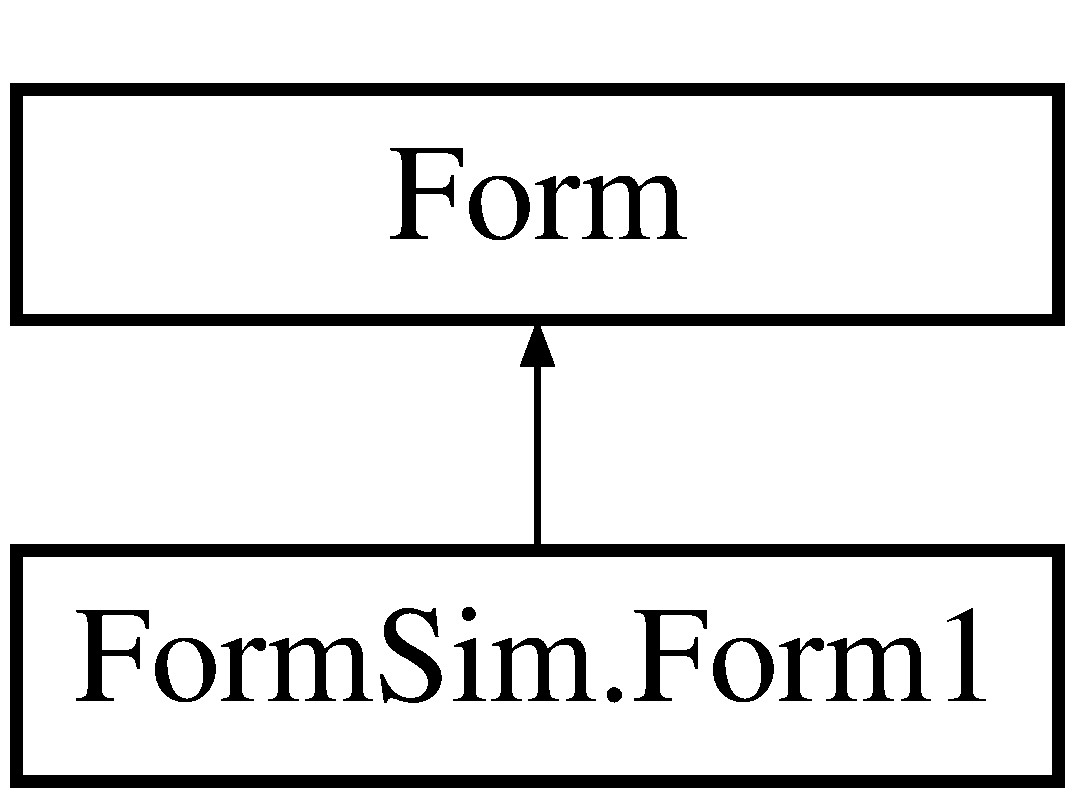
\includegraphics[height=2.000000cm]{class_form_sim_1_1_form1}
\end{center}
\end{figure}
\subsection*{Public Member Functions}
\begin{DoxyCompactItemize}
\item 
\mbox{\hyperlink{class_form_sim_1_1_form1_aaf140bd5cccdffe2b9f6c4a9b856b5ca}{Form1}} ()
\end{DoxyCompactItemize}
\subsection*{Protected Member Functions}
\begin{DoxyCompactItemize}
\item 
override void \mbox{\hyperlink{class_form_sim_1_1_form1_a5ab3d8b7fa32d3c15b3690d53104deae}{Dispose}} (bool disposing)
\begin{DoxyCompactList}\small\item\em Clean up any resources being used. \end{DoxyCompactList}\end{DoxyCompactItemize}
\subsection*{Private Member Functions}
\begin{DoxyCompactItemize}
\item 
async void \mbox{\hyperlink{class_form_sim_1_1_form1_a93df121074a9d4a5d84028c88006cd85}{Exchange\+Token\+\_\+\+Click\+Async}} (object sender, Event\+Args e)
\item 
async void \mbox{\hyperlink{class_form_sim_1_1_form1_a87ca4036b1c618f3093430405aeba8e4}{Send\+Transaction\+\_\+\+Click}} (object sender, Event\+Args e)
\item 
async void \mbox{\hyperlink{class_form_sim_1_1_form1_a084c2aeea3986cecad18ff155bdcf787}{Send\+Raw\+String\+\_\+\+Click}} (object sender, Event\+Args e)
\item 
void \mbox{\hyperlink{class_form_sim_1_1_form1_ad4bb652b7d70981d588fea85202d8141}{T\+C\+P\+\_\+\+Checked\+Changed}} (object sender, Event\+Args e)
\item 
void \mbox{\hyperlink{class_form_sim_1_1_form1_aefa5468c4118286a2ce65347ffb6e549}{H\+T\+T\+P\+\_\+\+Checked\+Changed}} (object sender, Event\+Args e)
\item 
void \mbox{\hyperlink{class_form_sim_1_1_form1_a1faf00c6508c7dd62d5f163c87bc1a2b}{T\+L\+S\+\_\+\+Checked\+Changed}} (object sender, Event\+Args e)
\item 
void \mbox{\hyperlink{class_form_sim_1_1_form1_abef6d6522b35a19fc08da5f6817d6190}{A\+P\+I\+Options\+Select\+\_\+\+Selected\+Index\+Changed}} (object sender, Event\+Args e)
\item 
string \mbox{\hyperlink{class_form_sim_1_1_form1_adddcbdfa223d8d3eea3710278d6f4825}{stripped}} (string str)
\item 
void \mbox{\hyperlink{class_form_sim_1_1_form1_a6d85c1197b7f08d87e53b0e326ee4375}{I\+P\+Address\+\_\+\+Selected\+Index\+Changed}} (object sender, Event\+Args e)
\item 
void \mbox{\hyperlink{class_form_sim_1_1_form1_acace7bb65973370b2802f93a43495e1b}{Mo\+To\+Ecom\+\_\+\+Checked\+Changed}} (object sender, Event\+Args e)
\item 
void \mbox{\hyperlink{class_form_sim_1_1_form1_af0c2817f4ba09eb6c2fb0fe6bee2457d}{Hotel\+\_\+\+Checked\+Changed}} (object sender, Event\+Args e)
\item 
void \mbox{\hyperlink{class_form_sim_1_1_form1_a7c36bc29aa6d9fc704fcee5fc434973c}{Food\+And\+Beverage\+\_\+\+Checked\+Changed}} (object sender, Event\+Args e)
\item 
void \mbox{\hyperlink{class_form_sim_1_1_form1_aa0ac63096f64895de6d57971386f8ee5}{Retail\+\_\+\+Checked\+Changed}} (object sender, Event\+Args e)
\item 
void \mbox{\hyperlink{class_form_sim_1_1_form1_adcc5acde3fe806f1d7f011e67626db1f}{Auto\+Rental\+\_\+\+Checked\+Changed}} (object sender, Event\+Args e)
\item 
delegate void \mbox{\hyperlink{class_form_sim_1_1_form1_a33ffcbbf1c37324badcb69a13ebef5e9}{String\+Arg\+Returning\+Void\+Delegate}} (string text)
\item 
void \mbox{\hyperlink{class_form_sim_1_1_form1_afd790c1181ee74c3b785002cdad0159c}{append\+Output}} (string text)
\item 
void \mbox{\hyperlink{class_form_sim_1_1_form1_a6e1199d3a12d5793d73ee11ef3ab7fc0}{set\+P2\+P\+E\+Text}} (string text)
\item 
void \mbox{\hyperlink{class_form_sim_1_1_form1_a68979f65b99bf8995c5cf842acb886f5}{Start\+I\+D\+Tech\+Devices\+\_\+\+Click}} (object sender, Event\+Args e)
\item 
void \mbox{\hyperlink{class_form_sim_1_1_form1_a1e61fd61ad2bdb7c5b75a9c0d138236b}{get\+Data}} ()
\item 
void \mbox{\hyperlink{class_form_sim_1_1_form1_af0bb58c8e4f2567486563b0b8c780538}{Initialize\+Component}} ()
\begin{DoxyCompactList}\small\item\em Required method for Designer support -\/ do not modify the contents of this method with the code editor. \end{DoxyCompactList}\end{DoxyCompactItemize}
\subsection*{Private Attributes}
\begin{DoxyCompactItemize}
\item 
\mbox{\hyperlink{interface_form_sim_1_1_f_r_c___handler}{F\+R\+C\+\_\+\+Handler}} \mbox{\hyperlink{class_form_sim_1_1_form1_a8dfc25cc1ba341fc90eedd2c4bc14e0a}{http\+Handler}}
\item 
\mbox{\hyperlink{interface_form_sim_1_1_f_r_c___handler}{F\+R\+C\+\_\+\+Handler}} \mbox{\hyperlink{class_form_sim_1_1_form1_acde1aeecb04378a845d95ff88cf3d040}{tcp\+Handler}}
\item 
\mbox{\hyperlink{interface_form_sim_1_1_f_r_c___handler}{F\+R\+C\+\_\+\+Handler}} \mbox{\hyperlink{class_form_sim_1_1_form1_ac99dc128e2000076182d609b9d5f6c03}{rest\+Handler}}
\item 
\mbox{\hyperlink{class_form_sim_1_1_helper}{Helper}} \mbox{\hyperlink{class_form_sim_1_1_form1_a358dd84324e5c41ae053e22b3de316b1}{helper}}
\item 
int \mbox{\hyperlink{class_form_sim_1_1_form1_a1d6628b9f5ec08a4fa980cd5645b8d29}{requestor\+Ref\+Num}}
\item 
System.\+Component\+Model.\+I\+Container \mbox{\hyperlink{class_form_sim_1_1_form1_a5a556548cf4184594e46a7f09272b157}{components}} = null
\begin{DoxyCompactList}\small\item\em Required designer variable. \end{DoxyCompactList}\item 
System.\+Windows.\+Forms.\+Group\+Box \mbox{\hyperlink{class_form_sim_1_1_form1_a47d1f14e566876f6b65baf0dcc0c654c}{Connection}}
\item 
System.\+Windows.\+Forms.\+Text\+Box \mbox{\hyperlink{class_form_sim_1_1_form1_a76e0d7892cbeb761e8a909ee121bbd28}{Port}}
\item 
System.\+Windows.\+Forms.\+Label \mbox{\hyperlink{class_form_sim_1_1_form1_a0c3a49d36dea620395d3cd1b59297e50}{label2}}
\item 
System.\+Windows.\+Forms.\+Label \mbox{\hyperlink{class_form_sim_1_1_form1_a34a318adef53671e5d6a190cb2059bb9}{label1}}
\item 
System.\+Windows.\+Forms.\+Group\+Box \mbox{\hyperlink{class_form_sim_1_1_form1_ae64d6539b6939fe353891f885c241d28}{T\+L\+S\+Settings}}
\item 
System.\+Windows.\+Forms.\+Radio\+Button \mbox{\hyperlink{class_form_sim_1_1_form1_a7a6e222c261c32e59d5b3fe4240d0a20}{T\+L\+S1\+\_\+2}}
\item 
System.\+Windows.\+Forms.\+Radio\+Button \mbox{\hyperlink{class_form_sim_1_1_form1_ad846aa3e6cfb67966ff72e360ad5896d}{T\+L\+S1\+\_\+0}}
\item 
System.\+Windows.\+Forms.\+Radio\+Button \mbox{\hyperlink{class_form_sim_1_1_form1_aa6bea49227d76f110c15b8ca5b58bc6b}{T\+L\+S1\+\_\+1}}
\item 
System.\+Windows.\+Forms.\+Radio\+Button \mbox{\hyperlink{class_form_sim_1_1_form1_a909569fd407fe0ddce10b6dc34a26f1e}{S\+S\+L3}}
\item 
System.\+Windows.\+Forms.\+Radio\+Button \mbox{\hyperlink{class_form_sim_1_1_form1_ad73a0aa5c4cfc71f0bba70eec1edfb92}{Any\+Supported}}
\item 
System.\+Windows.\+Forms.\+Check\+Box \mbox{\hyperlink{class_form_sim_1_1_form1_a3760928ef463d00f184c67c5b30355e9}{T\+LS}}
\item 
System.\+Windows.\+Forms.\+Radio\+Button \mbox{\hyperlink{class_form_sim_1_1_form1_a92e6dec54dfb1acfbb7a8f63f8489e43}{H\+T\+TP}}
\item 
System.\+Windows.\+Forms.\+Radio\+Button \mbox{\hyperlink{class_form_sim_1_1_form1_ad9d0a83e0e5b553c33946f7d08f61607}{T\+CP}}
\item 
System.\+Windows.\+Forms.\+Button \mbox{\hyperlink{class_form_sim_1_1_form1_a20db0b50c8258c0e32a51be1f70b706e}{Exchange\+Token}}
\item 
System.\+Windows.\+Forms.\+Text\+Box \mbox{\hyperlink{class_form_sim_1_1_form1_abdee1962ad29b235756c9217ae497b47}{Access\+Token}}
\item 
System.\+Windows.\+Forms.\+Label \mbox{\hyperlink{class_form_sim_1_1_form1_a9f8c85dcf7680bdc2cc5739e29d539ee}{label5}}
\item 
System.\+Windows.\+Forms.\+Text\+Box \mbox{\hyperlink{class_form_sim_1_1_form1_a9159fb7a54ec1f9912f5230f7cd21053}{Client\+G\+U\+ID}}
\item 
System.\+Windows.\+Forms.\+Label \mbox{\hyperlink{class_form_sim_1_1_form1_a3f3c4fcc79b7eeeee73a25153dbabb00}{label4}}
\item 
System.\+Windows.\+Forms.\+Label \mbox{\hyperlink{class_form_sim_1_1_form1_ae15fea51b38df18919dc31166bb31476}{label3}}
\item 
System.\+Windows.\+Forms.\+Text\+Box \mbox{\hyperlink{class_form_sim_1_1_form1_a9ded5796e52e8e26de24e566dd3aa7e2}{Auth\+Token}}
\item 
System.\+Windows.\+Forms.\+Text\+Box \mbox{\hyperlink{class_form_sim_1_1_form1_a4ef9ca660be8039828c8b8cb778770d4}{Output}}
\item 
System.\+Windows.\+Forms.\+Group\+Box \mbox{\hyperlink{class_form_sim_1_1_form1_aa2a4980aca0c0162f75dc47006579c5a}{group\+Box1}}
\item 
System.\+Windows.\+Forms.\+Button \mbox{\hyperlink{class_form_sim_1_1_form1_a25cf1c017027a578565ba3f5b6f1d999}{Send\+Transaction}}
\item 
System.\+Windows.\+Forms.\+Group\+Box \mbox{\hyperlink{class_form_sim_1_1_form1_a54b179ef9cabfd2e3e1838730a9ffb0b}{Card\+Data}}
\item 
System.\+Windows.\+Forms.\+Label \mbox{\hyperlink{class_form_sim_1_1_form1_ab544f40bb97ffdea24b6bace4ae4afc1}{label12}}
\item 
System.\+Windows.\+Forms.\+Combo\+Box \mbox{\hyperlink{class_form_sim_1_1_form1_af9522dc15f4938ce8468fa05ca8b1bd0}{Zip\+Code}}
\item 
System.\+Windows.\+Forms.\+Label \mbox{\hyperlink{class_form_sim_1_1_form1_a6f21487b9e8ff9baba33cda4fb0cd62c}{label11}}
\item 
System.\+Windows.\+Forms.\+Combo\+Box \mbox{\hyperlink{class_form_sim_1_1_form1_a81160df3bbe7347398f9a82ff66b1e13}{Street\+Address}}
\item 
System.\+Windows.\+Forms.\+Label \mbox{\hyperlink{class_form_sim_1_1_form1_adb8c4a009c6a2e7f4f0717a4b8fb7a14}{label10}}
\item 
System.\+Windows.\+Forms.\+Combo\+Box \mbox{\hyperlink{class_form_sim_1_1_form1_afe2488fe89c5a10df54ad5db76e2ae68}{C\+V\+V2}}
\item 
System.\+Windows.\+Forms.\+Label \mbox{\hyperlink{class_form_sim_1_1_form1_a931c11ada165f4111fdf92231d707ca8}{label9}}
\item 
System.\+Windows.\+Forms.\+Text\+Box \mbox{\hyperlink{class_form_sim_1_1_form1_aae3b97a32b9cc3f4585825becdda0ad8}{Expiration\+Year}}
\item 
System.\+Windows.\+Forms.\+Label \mbox{\hyperlink{class_form_sim_1_1_form1_a1335cd840952cd00c7d72d797cbb191e}{label8}}
\item 
System.\+Windows.\+Forms.\+Text\+Box \mbox{\hyperlink{class_form_sim_1_1_form1_ace6523c1c7c8f1c9f24a35137c1876bb}{Expiration\+Month}}
\item 
System.\+Windows.\+Forms.\+Label \mbox{\hyperlink{class_form_sim_1_1_form1_a3da1f60d5b86a5b470c6c901a9741bfc}{label7}}
\item 
System.\+Windows.\+Forms.\+Label \mbox{\hyperlink{class_form_sim_1_1_form1_a8874da97d5451e75fb5959216d038473}{label6}}
\item 
System.\+Windows.\+Forms.\+Combo\+Box \mbox{\hyperlink{class_form_sim_1_1_form1_a59d375ea0a88d92e37ca60a1758f0393}{Card\+Number}}
\item 
System.\+Windows.\+Forms.\+Combo\+Box \mbox{\hyperlink{class_form_sim_1_1_form1_a2e0b28b22c6ce97d2f980691e85b33c6}{Token\+Serial}}
\item 
System.\+Windows.\+Forms.\+Label \mbox{\hyperlink{class_form_sim_1_1_form1_a5ddc0a1b8a7e6e78cb6cbc43d73dc307}{label15}}
\item 
System.\+Windows.\+Forms.\+Combo\+Box \mbox{\hyperlink{class_form_sim_1_1_form1_ae61e0632600eb8b5d969ff4b0917ec87}{Unique\+ID}}
\item 
System.\+Windows.\+Forms.\+Label \mbox{\hyperlink{class_form_sim_1_1_form1_a3ca2ec314a631948f7a626a94025aee5}{label14}}
\item 
System.\+Windows.\+Forms.\+Combo\+Box \mbox{\hyperlink{class_form_sim_1_1_form1_a14c01f57c5847acb8b9989cdb59ff0a0}{Track\+Data}}
\item 
System.\+Windows.\+Forms.\+Label \mbox{\hyperlink{class_form_sim_1_1_form1_ac5456a8c4f7cb00b6b8584064af29b40}{label13}}
\item 
System.\+Windows.\+Forms.\+Group\+Box \mbox{\hyperlink{class_form_sim_1_1_form1_a9f2831eaf955dcf9f776b20903b6e487}{group\+Box2}}
\item 
System.\+Windows.\+Forms.\+List\+Box \mbox{\hyperlink{class_form_sim_1_1_form1_a05c5787e91c73340fa98391b1deda267}{A\+P\+I\+Options\+Select}}
\item 
System.\+Windows.\+Forms.\+Text\+Box \mbox{\hyperlink{class_form_sim_1_1_form1_a624a8c6064e2d2cb379a41185901f897}{A\+P\+I\+Options}}
\item 
System.\+Windows.\+Forms.\+Label \mbox{\hyperlink{class_form_sim_1_1_form1_a9335909ad1a4e1650f7fe6b9ec6204a4}{label16}}
\item 
System.\+Windows.\+Forms.\+Text\+Box \mbox{\hyperlink{class_form_sim_1_1_form1_ac5e5b6ff1f100057f95dc8ef2863e73d}{Invoice}}
\item 
System.\+Windows.\+Forms.\+Label \mbox{\hyperlink{class_form_sim_1_1_form1_a06b45b77a210d9aade9c7f8bc5f098cf}{label17}}
\item 
System.\+Windows.\+Forms.\+Text\+Box \mbox{\hyperlink{class_form_sim_1_1_form1_ade11df97d9e42cb5bfa48face25aee61}{Primary\+Cents}}
\item 
System.\+Windows.\+Forms.\+Label \mbox{\hyperlink{class_form_sim_1_1_form1_a2a0b326231f8846b6a83dad3412f1cd6}{label19}}
\item 
System.\+Windows.\+Forms.\+Text\+Box \mbox{\hyperlink{class_form_sim_1_1_form1_ac00a03177b1af62159eada44d2a44699}{Primary\+Dollars}}
\item 
System.\+Windows.\+Forms.\+Label \mbox{\hyperlink{class_form_sim_1_1_form1_adb515d22e99686454c195a2f64089cbe}{label18}}
\item 
System.\+Windows.\+Forms.\+Combo\+Box \mbox{\hyperlink{class_form_sim_1_1_form1_ad7fea37dd402b41276b2fa9171d87bc0}{Sale\+Flag}}
\item 
System.\+Windows.\+Forms.\+Label \mbox{\hyperlink{class_form_sim_1_1_form1_afe5b5e36f7e56440452b586f0ea7dfef}{label20}}
\item 
System.\+Windows.\+Forms.\+Text\+Box \mbox{\hyperlink{class_form_sim_1_1_form1_a38d06c622545714c91406e7dfbe66d1c}{Secondary\+Cents}}
\item 
System.\+Windows.\+Forms.\+Text\+Box \mbox{\hyperlink{class_form_sim_1_1_form1_a70a61c269f99aa95af780899fabfcae4}{Secondary\+Dollars}}
\item 
System.\+Windows.\+Forms.\+Label \mbox{\hyperlink{class_form_sim_1_1_form1_a76b64b05b919b6f3ff44d4050e4f324a}{label22}}
\item 
System.\+Windows.\+Forms.\+Label \mbox{\hyperlink{class_form_sim_1_1_form1_a79b50aa0c2268985b96ebdc05ccd7a6a}{label21}}
\item 
System.\+Windows.\+Forms.\+Combo\+Box \mbox{\hyperlink{class_form_sim_1_1_form1_a46991f1bba83499f54cf854581c14784}{Function\+Request\+Code}}
\item 
System.\+Windows.\+Forms.\+Label \mbox{\hyperlink{class_form_sim_1_1_form1_af3fa36a6dc94765d3232e0e22153931f}{label23}}
\item 
System.\+Windows.\+Forms.\+Text\+Box \mbox{\hyperlink{class_form_sim_1_1_form1_adafe0ffc98595ab2668679d46d356c49}{Tax\+Amount\+Cents}}
\item 
System.\+Windows.\+Forms.\+Text\+Box \mbox{\hyperlink{class_form_sim_1_1_form1_aa1c8e908bdeca81bd6e86283ce1dd7c4}{Tax\+Amount\+Dollars}}
\item 
System.\+Windows.\+Forms.\+Label \mbox{\hyperlink{class_form_sim_1_1_form1_a3a5cccb776db1488c5446ac9b7c94934}{label25}}
\item 
System.\+Windows.\+Forms.\+Label \mbox{\hyperlink{class_form_sim_1_1_form1_a82d2fc3992cd81f21563dfcd7c6a00d0}{label24}}
\item 
System.\+Windows.\+Forms.\+Check\+Box \mbox{\hyperlink{class_form_sim_1_1_form1_a98599689cde2b5935abc183f6d88c994}{Tax\+Indicator}}
\item 
System.\+Windows.\+Forms.\+Text\+Box \mbox{\hyperlink{class_form_sim_1_1_form1_a5b6c7bb34019bd75dac9c0c66849525c}{Tran\+ID}}
\item 
System.\+Windows.\+Forms.\+Label \mbox{\hyperlink{class_form_sim_1_1_form1_ad5910926bf8163bd586357327489fe97}{label26}}
\item 
System.\+Windows.\+Forms.\+Text\+Box \mbox{\hyperlink{class_form_sim_1_1_form1_a3467b3663809dc0058c06d4096195112}{Clerk}}
\item 
System.\+Windows.\+Forms.\+Label \mbox{\hyperlink{class_form_sim_1_1_form1_a79b7b1071294d3869f770027d2320995}{label27}}
\item 
System.\+Windows.\+Forms.\+Text\+Box \mbox{\hyperlink{class_form_sim_1_1_form1_a42e8c436f14385be46b7f8709842117b}{Terminal\+ID}}
\item 
System.\+Windows.\+Forms.\+Label \mbox{\hyperlink{class_form_sim_1_1_form1_a8ff3803f9d5326ff15be24c1ad63a26f}{label28}}
\item 
System.\+Windows.\+Forms.\+Group\+Box \mbox{\hyperlink{class_form_sim_1_1_form1_a5720ca856fb2951f607711dddb7d2c2c}{group\+Box3}}
\item 
System.\+Windows.\+Forms.\+Radio\+Button \mbox{\hyperlink{class_form_sim_1_1_form1_a11c72e62d927380d3886dc30a9bbccb5}{Unencrypted\+Track\+Data}}
\item 
System.\+Windows.\+Forms.\+Radio\+Button \mbox{\hyperlink{class_form_sim_1_1_form1_ae28b45eefe4dba9ab1e6a68aad9b69c5}{Unencrypted\+Card\+Data}}
\item 
System.\+Windows.\+Forms.\+Radio\+Button \mbox{\hyperlink{class_form_sim_1_1_form1_a487cd7322b02504424c07b0b0ed3d1c9}{P2\+PE}}
\item 
System.\+Windows.\+Forms.\+Radio\+Button \mbox{\hyperlink{class_form_sim_1_1_form1_ad2f26b2aa7f2d698ff06a10286b1f653}{True\+Token}}
\item 
System.\+Windows.\+Forms.\+Radio\+Button \mbox{\hyperlink{class_form_sim_1_1_form1_ac2750ba08d5ff215e33cbfbacd6c370d}{U\+T\+G\+Controlled\+P\+I\+N\+Pad}}
\item 
System.\+Windows.\+Forms.\+Check\+Box \mbox{\hyperlink{class_form_sim_1_1_form1_a22568fda606ce041b35f4a485b896edb}{Use\+Same\+Invoice}}
\item 
System.\+Windows.\+Forms.\+Group\+Box \mbox{\hyperlink{class_form_sim_1_1_form1_a1f197afbba156a1cd26e83d11b97d391}{group\+Box4}}
\item 
System.\+Windows.\+Forms.\+Check\+Box \mbox{\hyperlink{class_form_sim_1_1_form1_ae1cc93ed604fda928b9751fecf1d4873}{Void\+Invalid\+C\+V\+V2}}
\item 
System.\+Windows.\+Forms.\+Check\+Box \mbox{\hyperlink{class_form_sim_1_1_form1_aa0f74345c5136c35a702e5670cac3f3b}{Void\+Invalid\+A\+VS}}
\item 
System.\+Windows.\+Forms.\+Radio\+Button \mbox{\hyperlink{class_form_sim_1_1_form1_ac5c7fdaade4547605b5252b96334d107}{Mo\+To\+Ecom}}
\item 
System.\+Windows.\+Forms.\+Radio\+Button \mbox{\hyperlink{class_form_sim_1_1_form1_ad54c2a3dd2e3bc42c89b1f274e20bf11}{Auto\+Rental}}
\item 
System.\+Windows.\+Forms.\+Radio\+Button \mbox{\hyperlink{class_form_sim_1_1_form1_a5aaef580c721c58b391c31253d543ece}{Food\+And\+Beverage}}
\item 
System.\+Windows.\+Forms.\+Radio\+Button \mbox{\hyperlink{class_form_sim_1_1_form1_a0960c5bf8f82f7c1486da7d14b32cad8}{Hotel}}
\item 
System.\+Windows.\+Forms.\+Radio\+Button \mbox{\hyperlink{class_form_sim_1_1_form1_a5fdf9a5bfd8218662d2bec76b6b103b5}{Retail}}
\item 
System.\+Windows.\+Forms.\+Label \mbox{\hyperlink{class_form_sim_1_1_form1_a6344870b90caee4d8318e2748cc31763}{label29}}
\item 
System.\+Windows.\+Forms.\+Check\+Box \mbox{\hyperlink{class_form_sim_1_1_form1_a92373dcafbe3831980547e7b2c8aafb7}{Use\+Token\+Store}}
\item 
System.\+Windows.\+Forms.\+Check\+Box \mbox{\hyperlink{class_form_sim_1_1_form1_aa4f20d51107c4775cbe7f568638a1823}{Use\+Meta\+Token}}
\item 
System.\+Windows.\+Forms.\+Label \mbox{\hyperlink{class_form_sim_1_1_form1_ad2abdc434aaaf8a792447d008a21fbe2}{label30}}
\item 
System.\+Windows.\+Forms.\+Button \mbox{\hyperlink{class_form_sim_1_1_form1_a05953f1ae0702a0c19d215571d6e63b7}{Send\+Raw\+String}}
\item 
System.\+Windows.\+Forms.\+Label \mbox{\hyperlink{class_form_sim_1_1_form1_a950f80344811da3c7bc0f6846db75fbe}{label31}}
\item 
System.\+Windows.\+Forms.\+Text\+Box \mbox{\hyperlink{class_form_sim_1_1_form1_a508d427416f6dfb6a073293da2853ab0}{Customer\+Name}}
\item 
System.\+Windows.\+Forms.\+Check\+Box \mbox{\hyperlink{class_form_sim_1_1_form1_a031d77f0edc11783639640c5926222de}{Use\+Basic\+Tran\+Flow}}
\item 
System.\+Windows.\+Forms.\+Check\+Box \mbox{\hyperlink{class_form_sim_1_1_form1_a182b08b8cb893b9744845831b79c6fbd}{Use\+Rollbacks}}
\item 
System.\+Windows.\+Forms.\+Combo\+Box \mbox{\hyperlink{class_form_sim_1_1_form1_afbf09ae833347b353523d5a1ecef4084}{Card\+Type}}
\item 
System.\+Windows.\+Forms.\+Label \mbox{\hyperlink{class_form_sim_1_1_form1_ad0954b3637c21b4723d55b5be1cbebbe}{label32}}
\item 
System.\+Windows.\+Forms.\+Text\+Box \mbox{\hyperlink{class_form_sim_1_1_form1_a1599ed57c79662b977f3b13c88eee502}{Card\+Present}}
\item 
System.\+Windows.\+Forms.\+Combo\+Box \mbox{\hyperlink{class_form_sim_1_1_form1_ac09f0457ff2972d0a9274e7b0756682f}{I\+P\+Address}}
\item 
System.\+Windows.\+Forms.\+Button \mbox{\hyperlink{class_form_sim_1_1_form1_aea5b20a781fbb2efd0fbd5088a67aaaa}{Start\+I\+D\+Tech\+Devices}}
\item 
System.\+Windows.\+Forms.\+Radio\+Button \mbox{\hyperlink{class_form_sim_1_1_form1_a14067ff6c523d592fe72f29c399dbb2e}{Rest}}
\item 
System.\+Windows.\+Forms.\+Check\+Box \mbox{\hyperlink{class_form_sim_1_1_form1_ab6b0b12adccc16ecd16c7733a7e480ed}{Use\+Auth\+Capture}}
\item 
System.\+Windows.\+Forms.\+Check\+Box \mbox{\hyperlink{class_form_sim_1_1_form1_a19fbb1137bb7748a46e64c6b63e3059a}{Use\+E\+MV}}
\item 
System.\+Windows.\+Forms.\+Text\+Box \mbox{\hyperlink{class_form_sim_1_1_form1_a029d572a6091d81b931a2fc9358c4f67}{raw\+String}}
\end{DoxyCompactItemize}


\subsection{Constructor \& Destructor Documentation}
\mbox{\Hypertarget{class_form_sim_1_1_form1_aaf140bd5cccdffe2b9f6c4a9b856b5ca}\label{class_form_sim_1_1_form1_aaf140bd5cccdffe2b9f6c4a9b856b5ca}} 
\index{Form\+Sim\+::\+Form1@{Form\+Sim\+::\+Form1}!Form1@{Form1}}
\index{Form1@{Form1}!Form\+Sim\+::\+Form1@{Form\+Sim\+::\+Form1}}
\subsubsection{\texorpdfstring{Form1()}{Form1()}}
{\footnotesize\ttfamily Form\+Sim.\+Form1.\+Form1 (\begin{DoxyParamCaption}{ }\end{DoxyParamCaption})\hspace{0.3cm}{\ttfamily [inline]}}



\subsection{Member Function Documentation}
\mbox{\Hypertarget{class_form_sim_1_1_form1_abef6d6522b35a19fc08da5f6817d6190}\label{class_form_sim_1_1_form1_abef6d6522b35a19fc08da5f6817d6190}} 
\index{Form\+Sim\+::\+Form1@{Form\+Sim\+::\+Form1}!A\+P\+I\+Options\+Select\+\_\+\+Selected\+Index\+Changed@{A\+P\+I\+Options\+Select\+\_\+\+Selected\+Index\+Changed}}
\index{A\+P\+I\+Options\+Select\+\_\+\+Selected\+Index\+Changed@{A\+P\+I\+Options\+Select\+\_\+\+Selected\+Index\+Changed}!Form\+Sim\+::\+Form1@{Form\+Sim\+::\+Form1}}
\subsubsection{\texorpdfstring{A\+P\+I\+Options\+Select\+\_\+\+Selected\+Index\+Changed()}{APIOptionsSelect\_SelectedIndexChanged()}}
{\footnotesize\ttfamily void Form\+Sim.\+Form1.\+A\+P\+I\+Options\+Select\+\_\+\+Selected\+Index\+Changed (\begin{DoxyParamCaption}\item[{object}]{sender,  }\item[{Event\+Args}]{e }\end{DoxyParamCaption})\hspace{0.3cm}{\ttfamily [inline]}, {\ttfamily [private]}}

\mbox{\Hypertarget{class_form_sim_1_1_form1_afd790c1181ee74c3b785002cdad0159c}\label{class_form_sim_1_1_form1_afd790c1181ee74c3b785002cdad0159c}} 
\index{Form\+Sim\+::\+Form1@{Form\+Sim\+::\+Form1}!append\+Output@{append\+Output}}
\index{append\+Output@{append\+Output}!Form\+Sim\+::\+Form1@{Form\+Sim\+::\+Form1}}
\subsubsection{\texorpdfstring{append\+Output()}{appendOutput()}}
{\footnotesize\ttfamily void Form\+Sim.\+Form1.\+append\+Output (\begin{DoxyParamCaption}\item[{string}]{text }\end{DoxyParamCaption})\hspace{0.3cm}{\ttfamily [inline]}, {\ttfamily [private]}}

\mbox{\Hypertarget{class_form_sim_1_1_form1_adcc5acde3fe806f1d7f011e67626db1f}\label{class_form_sim_1_1_form1_adcc5acde3fe806f1d7f011e67626db1f}} 
\index{Form\+Sim\+::\+Form1@{Form\+Sim\+::\+Form1}!Auto\+Rental\+\_\+\+Checked\+Changed@{Auto\+Rental\+\_\+\+Checked\+Changed}}
\index{Auto\+Rental\+\_\+\+Checked\+Changed@{Auto\+Rental\+\_\+\+Checked\+Changed}!Form\+Sim\+::\+Form1@{Form\+Sim\+::\+Form1}}
\subsubsection{\texorpdfstring{Auto\+Rental\+\_\+\+Checked\+Changed()}{AutoRental\_CheckedChanged()}}
{\footnotesize\ttfamily void Form\+Sim.\+Form1.\+Auto\+Rental\+\_\+\+Checked\+Changed (\begin{DoxyParamCaption}\item[{object}]{sender,  }\item[{Event\+Args}]{e }\end{DoxyParamCaption})\hspace{0.3cm}{\ttfamily [inline]}, {\ttfamily [private]}}

\mbox{\Hypertarget{class_form_sim_1_1_form1_a5ab3d8b7fa32d3c15b3690d53104deae}\label{class_form_sim_1_1_form1_a5ab3d8b7fa32d3c15b3690d53104deae}} 
\index{Form\+Sim\+::\+Form1@{Form\+Sim\+::\+Form1}!Dispose@{Dispose}}
\index{Dispose@{Dispose}!Form\+Sim\+::\+Form1@{Form\+Sim\+::\+Form1}}
\subsubsection{\texorpdfstring{Dispose()}{Dispose()}}
{\footnotesize\ttfamily override void Form\+Sim.\+Form1.\+Dispose (\begin{DoxyParamCaption}\item[{bool}]{disposing }\end{DoxyParamCaption})\hspace{0.3cm}{\ttfamily [inline]}, {\ttfamily [protected]}}



Clean up any resources being used. 


\begin{DoxyParams}{Parameters}
{\em disposing} & true if managed resources should be disposed; otherwise, false.\\
\hline
\end{DoxyParams}
\mbox{\Hypertarget{class_form_sim_1_1_form1_a93df121074a9d4a5d84028c88006cd85}\label{class_form_sim_1_1_form1_a93df121074a9d4a5d84028c88006cd85}} 
\index{Form\+Sim\+::\+Form1@{Form\+Sim\+::\+Form1}!Exchange\+Token\+\_\+\+Click\+Async@{Exchange\+Token\+\_\+\+Click\+Async}}
\index{Exchange\+Token\+\_\+\+Click\+Async@{Exchange\+Token\+\_\+\+Click\+Async}!Form\+Sim\+::\+Form1@{Form\+Sim\+::\+Form1}}
\subsubsection{\texorpdfstring{Exchange\+Token\+\_\+\+Click\+Async()}{ExchangeToken\_ClickAsync()}}
{\footnotesize\ttfamily async void Form\+Sim.\+Form1.\+Exchange\+Token\+\_\+\+Click\+Async (\begin{DoxyParamCaption}\item[{object}]{sender,  }\item[{Event\+Args}]{e }\end{DoxyParamCaption})\hspace{0.3cm}{\ttfamily [inline]}, {\ttfamily [private]}}

\mbox{\Hypertarget{class_form_sim_1_1_form1_a7c36bc29aa6d9fc704fcee5fc434973c}\label{class_form_sim_1_1_form1_a7c36bc29aa6d9fc704fcee5fc434973c}} 
\index{Form\+Sim\+::\+Form1@{Form\+Sim\+::\+Form1}!Food\+And\+Beverage\+\_\+\+Checked\+Changed@{Food\+And\+Beverage\+\_\+\+Checked\+Changed}}
\index{Food\+And\+Beverage\+\_\+\+Checked\+Changed@{Food\+And\+Beverage\+\_\+\+Checked\+Changed}!Form\+Sim\+::\+Form1@{Form\+Sim\+::\+Form1}}
\subsubsection{\texorpdfstring{Food\+And\+Beverage\+\_\+\+Checked\+Changed()}{FoodAndBeverage\_CheckedChanged()}}
{\footnotesize\ttfamily void Form\+Sim.\+Form1.\+Food\+And\+Beverage\+\_\+\+Checked\+Changed (\begin{DoxyParamCaption}\item[{object}]{sender,  }\item[{Event\+Args}]{e }\end{DoxyParamCaption})\hspace{0.3cm}{\ttfamily [inline]}, {\ttfamily [private]}}

\mbox{\Hypertarget{class_form_sim_1_1_form1_a1e61fd61ad2bdb7c5b75a9c0d138236b}\label{class_form_sim_1_1_form1_a1e61fd61ad2bdb7c5b75a9c0d138236b}} 
\index{Form\+Sim\+::\+Form1@{Form\+Sim\+::\+Form1}!get\+Data@{get\+Data}}
\index{get\+Data@{get\+Data}!Form\+Sim\+::\+Form1@{Form\+Sim\+::\+Form1}}
\subsubsection{\texorpdfstring{get\+Data()}{getData()}}
{\footnotesize\ttfamily void Form\+Sim.\+Form1.\+get\+Data (\begin{DoxyParamCaption}{ }\end{DoxyParamCaption})\hspace{0.3cm}{\ttfamily [inline]}, {\ttfamily [private]}}

\mbox{\Hypertarget{class_form_sim_1_1_form1_af0c2817f4ba09eb6c2fb0fe6bee2457d}\label{class_form_sim_1_1_form1_af0c2817f4ba09eb6c2fb0fe6bee2457d}} 
\index{Form\+Sim\+::\+Form1@{Form\+Sim\+::\+Form1}!Hotel\+\_\+\+Checked\+Changed@{Hotel\+\_\+\+Checked\+Changed}}
\index{Hotel\+\_\+\+Checked\+Changed@{Hotel\+\_\+\+Checked\+Changed}!Form\+Sim\+::\+Form1@{Form\+Sim\+::\+Form1}}
\subsubsection{\texorpdfstring{Hotel\+\_\+\+Checked\+Changed()}{Hotel\_CheckedChanged()}}
{\footnotesize\ttfamily void Form\+Sim.\+Form1.\+Hotel\+\_\+\+Checked\+Changed (\begin{DoxyParamCaption}\item[{object}]{sender,  }\item[{Event\+Args}]{e }\end{DoxyParamCaption})\hspace{0.3cm}{\ttfamily [inline]}, {\ttfamily [private]}}

\mbox{\Hypertarget{class_form_sim_1_1_form1_aefa5468c4118286a2ce65347ffb6e549}\label{class_form_sim_1_1_form1_aefa5468c4118286a2ce65347ffb6e549}} 
\index{Form\+Sim\+::\+Form1@{Form\+Sim\+::\+Form1}!H\+T\+T\+P\+\_\+\+Checked\+Changed@{H\+T\+T\+P\+\_\+\+Checked\+Changed}}
\index{H\+T\+T\+P\+\_\+\+Checked\+Changed@{H\+T\+T\+P\+\_\+\+Checked\+Changed}!Form\+Sim\+::\+Form1@{Form\+Sim\+::\+Form1}}
\subsubsection{\texorpdfstring{H\+T\+T\+P\+\_\+\+Checked\+Changed()}{HTTP\_CheckedChanged()}}
{\footnotesize\ttfamily void Form\+Sim.\+Form1.\+H\+T\+T\+P\+\_\+\+Checked\+Changed (\begin{DoxyParamCaption}\item[{object}]{sender,  }\item[{Event\+Args}]{e }\end{DoxyParamCaption})\hspace{0.3cm}{\ttfamily [inline]}, {\ttfamily [private]}}

\mbox{\Hypertarget{class_form_sim_1_1_form1_af0bb58c8e4f2567486563b0b8c780538}\label{class_form_sim_1_1_form1_af0bb58c8e4f2567486563b0b8c780538}} 
\index{Form\+Sim\+::\+Form1@{Form\+Sim\+::\+Form1}!Initialize\+Component@{Initialize\+Component}}
\index{Initialize\+Component@{Initialize\+Component}!Form\+Sim\+::\+Form1@{Form\+Sim\+::\+Form1}}
\subsubsection{\texorpdfstring{Initialize\+Component()}{InitializeComponent()}}
{\footnotesize\ttfamily void Form\+Sim.\+Form1.\+Initialize\+Component (\begin{DoxyParamCaption}{ }\end{DoxyParamCaption})\hspace{0.3cm}{\ttfamily [inline]}, {\ttfamily [private]}}



Required method for Designer support -\/ do not modify the contents of this method with the code editor. 

\mbox{\Hypertarget{class_form_sim_1_1_form1_a6d85c1197b7f08d87e53b0e326ee4375}\label{class_form_sim_1_1_form1_a6d85c1197b7f08d87e53b0e326ee4375}} 
\index{Form\+Sim\+::\+Form1@{Form\+Sim\+::\+Form1}!I\+P\+Address\+\_\+\+Selected\+Index\+Changed@{I\+P\+Address\+\_\+\+Selected\+Index\+Changed}}
\index{I\+P\+Address\+\_\+\+Selected\+Index\+Changed@{I\+P\+Address\+\_\+\+Selected\+Index\+Changed}!Form\+Sim\+::\+Form1@{Form\+Sim\+::\+Form1}}
\subsubsection{\texorpdfstring{I\+P\+Address\+\_\+\+Selected\+Index\+Changed()}{IPAddress\_SelectedIndexChanged()}}
{\footnotesize\ttfamily void Form\+Sim.\+Form1.\+I\+P\+Address\+\_\+\+Selected\+Index\+Changed (\begin{DoxyParamCaption}\item[{object}]{sender,  }\item[{Event\+Args}]{e }\end{DoxyParamCaption})\hspace{0.3cm}{\ttfamily [inline]}, {\ttfamily [private]}}

\mbox{\Hypertarget{class_form_sim_1_1_form1_acace7bb65973370b2802f93a43495e1b}\label{class_form_sim_1_1_form1_acace7bb65973370b2802f93a43495e1b}} 
\index{Form\+Sim\+::\+Form1@{Form\+Sim\+::\+Form1}!Mo\+To\+Ecom\+\_\+\+Checked\+Changed@{Mo\+To\+Ecom\+\_\+\+Checked\+Changed}}
\index{Mo\+To\+Ecom\+\_\+\+Checked\+Changed@{Mo\+To\+Ecom\+\_\+\+Checked\+Changed}!Form\+Sim\+::\+Form1@{Form\+Sim\+::\+Form1}}
\subsubsection{\texorpdfstring{Mo\+To\+Ecom\+\_\+\+Checked\+Changed()}{MoToEcom\_CheckedChanged()}}
{\footnotesize\ttfamily void Form\+Sim.\+Form1.\+Mo\+To\+Ecom\+\_\+\+Checked\+Changed (\begin{DoxyParamCaption}\item[{object}]{sender,  }\item[{Event\+Args}]{e }\end{DoxyParamCaption})\hspace{0.3cm}{\ttfamily [inline]}, {\ttfamily [private]}}

\mbox{\Hypertarget{class_form_sim_1_1_form1_aa0ac63096f64895de6d57971386f8ee5}\label{class_form_sim_1_1_form1_aa0ac63096f64895de6d57971386f8ee5}} 
\index{Form\+Sim\+::\+Form1@{Form\+Sim\+::\+Form1}!Retail\+\_\+\+Checked\+Changed@{Retail\+\_\+\+Checked\+Changed}}
\index{Retail\+\_\+\+Checked\+Changed@{Retail\+\_\+\+Checked\+Changed}!Form\+Sim\+::\+Form1@{Form\+Sim\+::\+Form1}}
\subsubsection{\texorpdfstring{Retail\+\_\+\+Checked\+Changed()}{Retail\_CheckedChanged()}}
{\footnotesize\ttfamily void Form\+Sim.\+Form1.\+Retail\+\_\+\+Checked\+Changed (\begin{DoxyParamCaption}\item[{object}]{sender,  }\item[{Event\+Args}]{e }\end{DoxyParamCaption})\hspace{0.3cm}{\ttfamily [inline]}, {\ttfamily [private]}}

\mbox{\Hypertarget{class_form_sim_1_1_form1_a084c2aeea3986cecad18ff155bdcf787}\label{class_form_sim_1_1_form1_a084c2aeea3986cecad18ff155bdcf787}} 
\index{Form\+Sim\+::\+Form1@{Form\+Sim\+::\+Form1}!Send\+Raw\+String\+\_\+\+Click@{Send\+Raw\+String\+\_\+\+Click}}
\index{Send\+Raw\+String\+\_\+\+Click@{Send\+Raw\+String\+\_\+\+Click}!Form\+Sim\+::\+Form1@{Form\+Sim\+::\+Form1}}
\subsubsection{\texorpdfstring{Send\+Raw\+String\+\_\+\+Click()}{SendRawString\_Click()}}
{\footnotesize\ttfamily async void Form\+Sim.\+Form1.\+Send\+Raw\+String\+\_\+\+Click (\begin{DoxyParamCaption}\item[{object}]{sender,  }\item[{Event\+Args}]{e }\end{DoxyParamCaption})\hspace{0.3cm}{\ttfamily [inline]}, {\ttfamily [private]}}

\mbox{\Hypertarget{class_form_sim_1_1_form1_a87ca4036b1c618f3093430405aeba8e4}\label{class_form_sim_1_1_form1_a87ca4036b1c618f3093430405aeba8e4}} 
\index{Form\+Sim\+::\+Form1@{Form\+Sim\+::\+Form1}!Send\+Transaction\+\_\+\+Click@{Send\+Transaction\+\_\+\+Click}}
\index{Send\+Transaction\+\_\+\+Click@{Send\+Transaction\+\_\+\+Click}!Form\+Sim\+::\+Form1@{Form\+Sim\+::\+Form1}}
\subsubsection{\texorpdfstring{Send\+Transaction\+\_\+\+Click()}{SendTransaction\_Click()}}
{\footnotesize\ttfamily async void Form\+Sim.\+Form1.\+Send\+Transaction\+\_\+\+Click (\begin{DoxyParamCaption}\item[{object}]{sender,  }\item[{Event\+Args}]{e }\end{DoxyParamCaption})\hspace{0.3cm}{\ttfamily [inline]}, {\ttfamily [private]}}

\mbox{\Hypertarget{class_form_sim_1_1_form1_a6e1199d3a12d5793d73ee11ef3ab7fc0}\label{class_form_sim_1_1_form1_a6e1199d3a12d5793d73ee11ef3ab7fc0}} 
\index{Form\+Sim\+::\+Form1@{Form\+Sim\+::\+Form1}!set\+P2\+P\+E\+Text@{set\+P2\+P\+E\+Text}}
\index{set\+P2\+P\+E\+Text@{set\+P2\+P\+E\+Text}!Form\+Sim\+::\+Form1@{Form\+Sim\+::\+Form1}}
\subsubsection{\texorpdfstring{set\+P2\+P\+E\+Text()}{setP2PEText()}}
{\footnotesize\ttfamily void Form\+Sim.\+Form1.\+set\+P2\+P\+E\+Text (\begin{DoxyParamCaption}\item[{string}]{text }\end{DoxyParamCaption})\hspace{0.3cm}{\ttfamily [inline]}, {\ttfamily [private]}}

\mbox{\Hypertarget{class_form_sim_1_1_form1_a68979f65b99bf8995c5cf842acb886f5}\label{class_form_sim_1_1_form1_a68979f65b99bf8995c5cf842acb886f5}} 
\index{Form\+Sim\+::\+Form1@{Form\+Sim\+::\+Form1}!Start\+I\+D\+Tech\+Devices\+\_\+\+Click@{Start\+I\+D\+Tech\+Devices\+\_\+\+Click}}
\index{Start\+I\+D\+Tech\+Devices\+\_\+\+Click@{Start\+I\+D\+Tech\+Devices\+\_\+\+Click}!Form\+Sim\+::\+Form1@{Form\+Sim\+::\+Form1}}
\subsubsection{\texorpdfstring{Start\+I\+D\+Tech\+Devices\+\_\+\+Click()}{StartIDTechDevices\_Click()}}
{\footnotesize\ttfamily void Form\+Sim.\+Form1.\+Start\+I\+D\+Tech\+Devices\+\_\+\+Click (\begin{DoxyParamCaption}\item[{object}]{sender,  }\item[{Event\+Args}]{e }\end{DoxyParamCaption})\hspace{0.3cm}{\ttfamily [inline]}, {\ttfamily [private]}}

\mbox{\Hypertarget{class_form_sim_1_1_form1_a33ffcbbf1c37324badcb69a13ebef5e9}\label{class_form_sim_1_1_form1_a33ffcbbf1c37324badcb69a13ebef5e9}} 
\index{Form\+Sim\+::\+Form1@{Form\+Sim\+::\+Form1}!String\+Arg\+Returning\+Void\+Delegate@{String\+Arg\+Returning\+Void\+Delegate}}
\index{String\+Arg\+Returning\+Void\+Delegate@{String\+Arg\+Returning\+Void\+Delegate}!Form\+Sim\+::\+Form1@{Form\+Sim\+::\+Form1}}
\subsubsection{\texorpdfstring{String\+Arg\+Returning\+Void\+Delegate()}{StringArgReturningVoidDelegate()}}
{\footnotesize\ttfamily delegate void Form\+Sim.\+Form1.\+String\+Arg\+Returning\+Void\+Delegate (\begin{DoxyParamCaption}\item[{string}]{text }\end{DoxyParamCaption})\hspace{0.3cm}{\ttfamily [private]}}

\mbox{\Hypertarget{class_form_sim_1_1_form1_adddcbdfa223d8d3eea3710278d6f4825}\label{class_form_sim_1_1_form1_adddcbdfa223d8d3eea3710278d6f4825}} 
\index{Form\+Sim\+::\+Form1@{Form\+Sim\+::\+Form1}!stripped@{stripped}}
\index{stripped@{stripped}!Form\+Sim\+::\+Form1@{Form\+Sim\+::\+Form1}}
\subsubsection{\texorpdfstring{stripped()}{stripped()}}
{\footnotesize\ttfamily string Form\+Sim.\+Form1.\+stripped (\begin{DoxyParamCaption}\item[{string}]{str }\end{DoxyParamCaption})\hspace{0.3cm}{\ttfamily [inline]}, {\ttfamily [private]}}

\mbox{\Hypertarget{class_form_sim_1_1_form1_ad4bb652b7d70981d588fea85202d8141}\label{class_form_sim_1_1_form1_ad4bb652b7d70981d588fea85202d8141}} 
\index{Form\+Sim\+::\+Form1@{Form\+Sim\+::\+Form1}!T\+C\+P\+\_\+\+Checked\+Changed@{T\+C\+P\+\_\+\+Checked\+Changed}}
\index{T\+C\+P\+\_\+\+Checked\+Changed@{T\+C\+P\+\_\+\+Checked\+Changed}!Form\+Sim\+::\+Form1@{Form\+Sim\+::\+Form1}}
\subsubsection{\texorpdfstring{T\+C\+P\+\_\+\+Checked\+Changed()}{TCP\_CheckedChanged()}}
{\footnotesize\ttfamily void Form\+Sim.\+Form1.\+T\+C\+P\+\_\+\+Checked\+Changed (\begin{DoxyParamCaption}\item[{object}]{sender,  }\item[{Event\+Args}]{e }\end{DoxyParamCaption})\hspace{0.3cm}{\ttfamily [inline]}, {\ttfamily [private]}}

\mbox{\Hypertarget{class_form_sim_1_1_form1_a1faf00c6508c7dd62d5f163c87bc1a2b}\label{class_form_sim_1_1_form1_a1faf00c6508c7dd62d5f163c87bc1a2b}} 
\index{Form\+Sim\+::\+Form1@{Form\+Sim\+::\+Form1}!T\+L\+S\+\_\+\+Checked\+Changed@{T\+L\+S\+\_\+\+Checked\+Changed}}
\index{T\+L\+S\+\_\+\+Checked\+Changed@{T\+L\+S\+\_\+\+Checked\+Changed}!Form\+Sim\+::\+Form1@{Form\+Sim\+::\+Form1}}
\subsubsection{\texorpdfstring{T\+L\+S\+\_\+\+Checked\+Changed()}{TLS\_CheckedChanged()}}
{\footnotesize\ttfamily void Form\+Sim.\+Form1.\+T\+L\+S\+\_\+\+Checked\+Changed (\begin{DoxyParamCaption}\item[{object}]{sender,  }\item[{Event\+Args}]{e }\end{DoxyParamCaption})\hspace{0.3cm}{\ttfamily [inline]}, {\ttfamily [private]}}



\subsection{Member Data Documentation}
\mbox{\Hypertarget{class_form_sim_1_1_form1_abdee1962ad29b235756c9217ae497b47}\label{class_form_sim_1_1_form1_abdee1962ad29b235756c9217ae497b47}} 
\index{Form\+Sim\+::\+Form1@{Form\+Sim\+::\+Form1}!Access\+Token@{Access\+Token}}
\index{Access\+Token@{Access\+Token}!Form\+Sim\+::\+Form1@{Form\+Sim\+::\+Form1}}
\subsubsection{\texorpdfstring{Access\+Token}{AccessToken}}
{\footnotesize\ttfamily System.\+Windows.\+Forms.\+Text\+Box Form\+Sim.\+Form1.\+Access\+Token\hspace{0.3cm}{\ttfamily [private]}}

\mbox{\Hypertarget{class_form_sim_1_1_form1_ad73a0aa5c4cfc71f0bba70eec1edfb92}\label{class_form_sim_1_1_form1_ad73a0aa5c4cfc71f0bba70eec1edfb92}} 
\index{Form\+Sim\+::\+Form1@{Form\+Sim\+::\+Form1}!Any\+Supported@{Any\+Supported}}
\index{Any\+Supported@{Any\+Supported}!Form\+Sim\+::\+Form1@{Form\+Sim\+::\+Form1}}
\subsubsection{\texorpdfstring{Any\+Supported}{AnySupported}}
{\footnotesize\ttfamily System.\+Windows.\+Forms.\+Radio\+Button Form\+Sim.\+Form1.\+Any\+Supported\hspace{0.3cm}{\ttfamily [private]}}

\mbox{\Hypertarget{class_form_sim_1_1_form1_a624a8c6064e2d2cb379a41185901f897}\label{class_form_sim_1_1_form1_a624a8c6064e2d2cb379a41185901f897}} 
\index{Form\+Sim\+::\+Form1@{Form\+Sim\+::\+Form1}!A\+P\+I\+Options@{A\+P\+I\+Options}}
\index{A\+P\+I\+Options@{A\+P\+I\+Options}!Form\+Sim\+::\+Form1@{Form\+Sim\+::\+Form1}}
\subsubsection{\texorpdfstring{A\+P\+I\+Options}{APIOptions}}
{\footnotesize\ttfamily System.\+Windows.\+Forms.\+Text\+Box Form\+Sim.\+Form1.\+A\+P\+I\+Options\hspace{0.3cm}{\ttfamily [private]}}

\mbox{\Hypertarget{class_form_sim_1_1_form1_a05c5787e91c73340fa98391b1deda267}\label{class_form_sim_1_1_form1_a05c5787e91c73340fa98391b1deda267}} 
\index{Form\+Sim\+::\+Form1@{Form\+Sim\+::\+Form1}!A\+P\+I\+Options\+Select@{A\+P\+I\+Options\+Select}}
\index{A\+P\+I\+Options\+Select@{A\+P\+I\+Options\+Select}!Form\+Sim\+::\+Form1@{Form\+Sim\+::\+Form1}}
\subsubsection{\texorpdfstring{A\+P\+I\+Options\+Select}{APIOptionsSelect}}
{\footnotesize\ttfamily System.\+Windows.\+Forms.\+List\+Box Form\+Sim.\+Form1.\+A\+P\+I\+Options\+Select\hspace{0.3cm}{\ttfamily [private]}}

\mbox{\Hypertarget{class_form_sim_1_1_form1_a9ded5796e52e8e26de24e566dd3aa7e2}\label{class_form_sim_1_1_form1_a9ded5796e52e8e26de24e566dd3aa7e2}} 
\index{Form\+Sim\+::\+Form1@{Form\+Sim\+::\+Form1}!Auth\+Token@{Auth\+Token}}
\index{Auth\+Token@{Auth\+Token}!Form\+Sim\+::\+Form1@{Form\+Sim\+::\+Form1}}
\subsubsection{\texorpdfstring{Auth\+Token}{AuthToken}}
{\footnotesize\ttfamily System.\+Windows.\+Forms.\+Text\+Box Form\+Sim.\+Form1.\+Auth\+Token\hspace{0.3cm}{\ttfamily [private]}}

\mbox{\Hypertarget{class_form_sim_1_1_form1_ad54c2a3dd2e3bc42c89b1f274e20bf11}\label{class_form_sim_1_1_form1_ad54c2a3dd2e3bc42c89b1f274e20bf11}} 
\index{Form\+Sim\+::\+Form1@{Form\+Sim\+::\+Form1}!Auto\+Rental@{Auto\+Rental}}
\index{Auto\+Rental@{Auto\+Rental}!Form\+Sim\+::\+Form1@{Form\+Sim\+::\+Form1}}
\subsubsection{\texorpdfstring{Auto\+Rental}{AutoRental}}
{\footnotesize\ttfamily System.\+Windows.\+Forms.\+Radio\+Button Form\+Sim.\+Form1.\+Auto\+Rental\hspace{0.3cm}{\ttfamily [private]}}

\mbox{\Hypertarget{class_form_sim_1_1_form1_a54b179ef9cabfd2e3e1838730a9ffb0b}\label{class_form_sim_1_1_form1_a54b179ef9cabfd2e3e1838730a9ffb0b}} 
\index{Form\+Sim\+::\+Form1@{Form\+Sim\+::\+Form1}!Card\+Data@{Card\+Data}}
\index{Card\+Data@{Card\+Data}!Form\+Sim\+::\+Form1@{Form\+Sim\+::\+Form1}}
\subsubsection{\texorpdfstring{Card\+Data}{CardData}}
{\footnotesize\ttfamily System.\+Windows.\+Forms.\+Group\+Box Form\+Sim.\+Form1.\+Card\+Data\hspace{0.3cm}{\ttfamily [private]}}

\mbox{\Hypertarget{class_form_sim_1_1_form1_a59d375ea0a88d92e37ca60a1758f0393}\label{class_form_sim_1_1_form1_a59d375ea0a88d92e37ca60a1758f0393}} 
\index{Form\+Sim\+::\+Form1@{Form\+Sim\+::\+Form1}!Card\+Number@{Card\+Number}}
\index{Card\+Number@{Card\+Number}!Form\+Sim\+::\+Form1@{Form\+Sim\+::\+Form1}}
\subsubsection{\texorpdfstring{Card\+Number}{CardNumber}}
{\footnotesize\ttfamily System.\+Windows.\+Forms.\+Combo\+Box Form\+Sim.\+Form1.\+Card\+Number\hspace{0.3cm}{\ttfamily [private]}}

\mbox{\Hypertarget{class_form_sim_1_1_form1_a1599ed57c79662b977f3b13c88eee502}\label{class_form_sim_1_1_form1_a1599ed57c79662b977f3b13c88eee502}} 
\index{Form\+Sim\+::\+Form1@{Form\+Sim\+::\+Form1}!Card\+Present@{Card\+Present}}
\index{Card\+Present@{Card\+Present}!Form\+Sim\+::\+Form1@{Form\+Sim\+::\+Form1}}
\subsubsection{\texorpdfstring{Card\+Present}{CardPresent}}
{\footnotesize\ttfamily System.\+Windows.\+Forms.\+Text\+Box Form\+Sim.\+Form1.\+Card\+Present\hspace{0.3cm}{\ttfamily [private]}}

\mbox{\Hypertarget{class_form_sim_1_1_form1_afbf09ae833347b353523d5a1ecef4084}\label{class_form_sim_1_1_form1_afbf09ae833347b353523d5a1ecef4084}} 
\index{Form\+Sim\+::\+Form1@{Form\+Sim\+::\+Form1}!Card\+Type@{Card\+Type}}
\index{Card\+Type@{Card\+Type}!Form\+Sim\+::\+Form1@{Form\+Sim\+::\+Form1}}
\subsubsection{\texorpdfstring{Card\+Type}{CardType}}
{\footnotesize\ttfamily System.\+Windows.\+Forms.\+Combo\+Box Form\+Sim.\+Form1.\+Card\+Type\hspace{0.3cm}{\ttfamily [private]}}

\mbox{\Hypertarget{class_form_sim_1_1_form1_a3467b3663809dc0058c06d4096195112}\label{class_form_sim_1_1_form1_a3467b3663809dc0058c06d4096195112}} 
\index{Form\+Sim\+::\+Form1@{Form\+Sim\+::\+Form1}!Clerk@{Clerk}}
\index{Clerk@{Clerk}!Form\+Sim\+::\+Form1@{Form\+Sim\+::\+Form1}}
\subsubsection{\texorpdfstring{Clerk}{Clerk}}
{\footnotesize\ttfamily System.\+Windows.\+Forms.\+Text\+Box Form\+Sim.\+Form1.\+Clerk\hspace{0.3cm}{\ttfamily [private]}}

\mbox{\Hypertarget{class_form_sim_1_1_form1_a9159fb7a54ec1f9912f5230f7cd21053}\label{class_form_sim_1_1_form1_a9159fb7a54ec1f9912f5230f7cd21053}} 
\index{Form\+Sim\+::\+Form1@{Form\+Sim\+::\+Form1}!Client\+G\+U\+ID@{Client\+G\+U\+ID}}
\index{Client\+G\+U\+ID@{Client\+G\+U\+ID}!Form\+Sim\+::\+Form1@{Form\+Sim\+::\+Form1}}
\subsubsection{\texorpdfstring{Client\+G\+U\+ID}{ClientGUID}}
{\footnotesize\ttfamily System.\+Windows.\+Forms.\+Text\+Box Form\+Sim.\+Form1.\+Client\+G\+U\+ID\hspace{0.3cm}{\ttfamily [private]}}

\mbox{\Hypertarget{class_form_sim_1_1_form1_a5a556548cf4184594e46a7f09272b157}\label{class_form_sim_1_1_form1_a5a556548cf4184594e46a7f09272b157}} 
\index{Form\+Sim\+::\+Form1@{Form\+Sim\+::\+Form1}!components@{components}}
\index{components@{components}!Form\+Sim\+::\+Form1@{Form\+Sim\+::\+Form1}}
\subsubsection{\texorpdfstring{components}{components}}
{\footnotesize\ttfamily System.\+Component\+Model.\+I\+Container Form\+Sim.\+Form1.\+components = null\hspace{0.3cm}{\ttfamily [private]}}



Required designer variable. 

\mbox{\Hypertarget{class_form_sim_1_1_form1_a47d1f14e566876f6b65baf0dcc0c654c}\label{class_form_sim_1_1_form1_a47d1f14e566876f6b65baf0dcc0c654c}} 
\index{Form\+Sim\+::\+Form1@{Form\+Sim\+::\+Form1}!Connection@{Connection}}
\index{Connection@{Connection}!Form\+Sim\+::\+Form1@{Form\+Sim\+::\+Form1}}
\subsubsection{\texorpdfstring{Connection}{Connection}}
{\footnotesize\ttfamily System.\+Windows.\+Forms.\+Group\+Box Form\+Sim.\+Form1.\+Connection\hspace{0.3cm}{\ttfamily [private]}}

\mbox{\Hypertarget{class_form_sim_1_1_form1_a508d427416f6dfb6a073293da2853ab0}\label{class_form_sim_1_1_form1_a508d427416f6dfb6a073293da2853ab0}} 
\index{Form\+Sim\+::\+Form1@{Form\+Sim\+::\+Form1}!Customer\+Name@{Customer\+Name}}
\index{Customer\+Name@{Customer\+Name}!Form\+Sim\+::\+Form1@{Form\+Sim\+::\+Form1}}
\subsubsection{\texorpdfstring{Customer\+Name}{CustomerName}}
{\footnotesize\ttfamily System.\+Windows.\+Forms.\+Text\+Box Form\+Sim.\+Form1.\+Customer\+Name\hspace{0.3cm}{\ttfamily [private]}}

\mbox{\Hypertarget{class_form_sim_1_1_form1_afe2488fe89c5a10df54ad5db76e2ae68}\label{class_form_sim_1_1_form1_afe2488fe89c5a10df54ad5db76e2ae68}} 
\index{Form\+Sim\+::\+Form1@{Form\+Sim\+::\+Form1}!C\+V\+V2@{C\+V\+V2}}
\index{C\+V\+V2@{C\+V\+V2}!Form\+Sim\+::\+Form1@{Form\+Sim\+::\+Form1}}
\subsubsection{\texorpdfstring{C\+V\+V2}{CVV2}}
{\footnotesize\ttfamily System.\+Windows.\+Forms.\+Combo\+Box Form\+Sim.\+Form1.\+C\+V\+V2\hspace{0.3cm}{\ttfamily [private]}}

\mbox{\Hypertarget{class_form_sim_1_1_form1_a20db0b50c8258c0e32a51be1f70b706e}\label{class_form_sim_1_1_form1_a20db0b50c8258c0e32a51be1f70b706e}} 
\index{Form\+Sim\+::\+Form1@{Form\+Sim\+::\+Form1}!Exchange\+Token@{Exchange\+Token}}
\index{Exchange\+Token@{Exchange\+Token}!Form\+Sim\+::\+Form1@{Form\+Sim\+::\+Form1}}
\subsubsection{\texorpdfstring{Exchange\+Token}{ExchangeToken}}
{\footnotesize\ttfamily System.\+Windows.\+Forms.\+Button Form\+Sim.\+Form1.\+Exchange\+Token\hspace{0.3cm}{\ttfamily [private]}}

\mbox{\Hypertarget{class_form_sim_1_1_form1_ace6523c1c7c8f1c9f24a35137c1876bb}\label{class_form_sim_1_1_form1_ace6523c1c7c8f1c9f24a35137c1876bb}} 
\index{Form\+Sim\+::\+Form1@{Form\+Sim\+::\+Form1}!Expiration\+Month@{Expiration\+Month}}
\index{Expiration\+Month@{Expiration\+Month}!Form\+Sim\+::\+Form1@{Form\+Sim\+::\+Form1}}
\subsubsection{\texorpdfstring{Expiration\+Month}{ExpirationMonth}}
{\footnotesize\ttfamily System.\+Windows.\+Forms.\+Text\+Box Form\+Sim.\+Form1.\+Expiration\+Month\hspace{0.3cm}{\ttfamily [private]}}

\mbox{\Hypertarget{class_form_sim_1_1_form1_aae3b97a32b9cc3f4585825becdda0ad8}\label{class_form_sim_1_1_form1_aae3b97a32b9cc3f4585825becdda0ad8}} 
\index{Form\+Sim\+::\+Form1@{Form\+Sim\+::\+Form1}!Expiration\+Year@{Expiration\+Year}}
\index{Expiration\+Year@{Expiration\+Year}!Form\+Sim\+::\+Form1@{Form\+Sim\+::\+Form1}}
\subsubsection{\texorpdfstring{Expiration\+Year}{ExpirationYear}}
{\footnotesize\ttfamily System.\+Windows.\+Forms.\+Text\+Box Form\+Sim.\+Form1.\+Expiration\+Year\hspace{0.3cm}{\ttfamily [private]}}

\mbox{\Hypertarget{class_form_sim_1_1_form1_a5aaef580c721c58b391c31253d543ece}\label{class_form_sim_1_1_form1_a5aaef580c721c58b391c31253d543ece}} 
\index{Form\+Sim\+::\+Form1@{Form\+Sim\+::\+Form1}!Food\+And\+Beverage@{Food\+And\+Beverage}}
\index{Food\+And\+Beverage@{Food\+And\+Beverage}!Form\+Sim\+::\+Form1@{Form\+Sim\+::\+Form1}}
\subsubsection{\texorpdfstring{Food\+And\+Beverage}{FoodAndBeverage}}
{\footnotesize\ttfamily System.\+Windows.\+Forms.\+Radio\+Button Form\+Sim.\+Form1.\+Food\+And\+Beverage\hspace{0.3cm}{\ttfamily [private]}}

\mbox{\Hypertarget{class_form_sim_1_1_form1_a46991f1bba83499f54cf854581c14784}\label{class_form_sim_1_1_form1_a46991f1bba83499f54cf854581c14784}} 
\index{Form\+Sim\+::\+Form1@{Form\+Sim\+::\+Form1}!Function\+Request\+Code@{Function\+Request\+Code}}
\index{Function\+Request\+Code@{Function\+Request\+Code}!Form\+Sim\+::\+Form1@{Form\+Sim\+::\+Form1}}
\subsubsection{\texorpdfstring{Function\+Request\+Code}{FunctionRequestCode}}
{\footnotesize\ttfamily System.\+Windows.\+Forms.\+Combo\+Box Form\+Sim.\+Form1.\+Function\+Request\+Code\hspace{0.3cm}{\ttfamily [private]}}

\mbox{\Hypertarget{class_form_sim_1_1_form1_aa2a4980aca0c0162f75dc47006579c5a}\label{class_form_sim_1_1_form1_aa2a4980aca0c0162f75dc47006579c5a}} 
\index{Form\+Sim\+::\+Form1@{Form\+Sim\+::\+Form1}!group\+Box1@{group\+Box1}}
\index{group\+Box1@{group\+Box1}!Form\+Sim\+::\+Form1@{Form\+Sim\+::\+Form1}}
\subsubsection{\texorpdfstring{group\+Box1}{groupBox1}}
{\footnotesize\ttfamily System.\+Windows.\+Forms.\+Group\+Box Form\+Sim.\+Form1.\+group\+Box1\hspace{0.3cm}{\ttfamily [private]}}

\mbox{\Hypertarget{class_form_sim_1_1_form1_a9f2831eaf955dcf9f776b20903b6e487}\label{class_form_sim_1_1_form1_a9f2831eaf955dcf9f776b20903b6e487}} 
\index{Form\+Sim\+::\+Form1@{Form\+Sim\+::\+Form1}!group\+Box2@{group\+Box2}}
\index{group\+Box2@{group\+Box2}!Form\+Sim\+::\+Form1@{Form\+Sim\+::\+Form1}}
\subsubsection{\texorpdfstring{group\+Box2}{groupBox2}}
{\footnotesize\ttfamily System.\+Windows.\+Forms.\+Group\+Box Form\+Sim.\+Form1.\+group\+Box2\hspace{0.3cm}{\ttfamily [private]}}

\mbox{\Hypertarget{class_form_sim_1_1_form1_a5720ca856fb2951f607711dddb7d2c2c}\label{class_form_sim_1_1_form1_a5720ca856fb2951f607711dddb7d2c2c}} 
\index{Form\+Sim\+::\+Form1@{Form\+Sim\+::\+Form1}!group\+Box3@{group\+Box3}}
\index{group\+Box3@{group\+Box3}!Form\+Sim\+::\+Form1@{Form\+Sim\+::\+Form1}}
\subsubsection{\texorpdfstring{group\+Box3}{groupBox3}}
{\footnotesize\ttfamily System.\+Windows.\+Forms.\+Group\+Box Form\+Sim.\+Form1.\+group\+Box3\hspace{0.3cm}{\ttfamily [private]}}

\mbox{\Hypertarget{class_form_sim_1_1_form1_a1f197afbba156a1cd26e83d11b97d391}\label{class_form_sim_1_1_form1_a1f197afbba156a1cd26e83d11b97d391}} 
\index{Form\+Sim\+::\+Form1@{Form\+Sim\+::\+Form1}!group\+Box4@{group\+Box4}}
\index{group\+Box4@{group\+Box4}!Form\+Sim\+::\+Form1@{Form\+Sim\+::\+Form1}}
\subsubsection{\texorpdfstring{group\+Box4}{groupBox4}}
{\footnotesize\ttfamily System.\+Windows.\+Forms.\+Group\+Box Form\+Sim.\+Form1.\+group\+Box4\hspace{0.3cm}{\ttfamily [private]}}

\mbox{\Hypertarget{class_form_sim_1_1_form1_a358dd84324e5c41ae053e22b3de316b1}\label{class_form_sim_1_1_form1_a358dd84324e5c41ae053e22b3de316b1}} 
\index{Form\+Sim\+::\+Form1@{Form\+Sim\+::\+Form1}!helper@{helper}}
\index{helper@{helper}!Form\+Sim\+::\+Form1@{Form\+Sim\+::\+Form1}}
\subsubsection{\texorpdfstring{helper}{helper}}
{\footnotesize\ttfamily \mbox{\hyperlink{class_form_sim_1_1_helper}{Helper}} Form\+Sim.\+Form1.\+helper\hspace{0.3cm}{\ttfamily [private]}}

\mbox{\Hypertarget{class_form_sim_1_1_form1_a0960c5bf8f82f7c1486da7d14b32cad8}\label{class_form_sim_1_1_form1_a0960c5bf8f82f7c1486da7d14b32cad8}} 
\index{Form\+Sim\+::\+Form1@{Form\+Sim\+::\+Form1}!Hotel@{Hotel}}
\index{Hotel@{Hotel}!Form\+Sim\+::\+Form1@{Form\+Sim\+::\+Form1}}
\subsubsection{\texorpdfstring{Hotel}{Hotel}}
{\footnotesize\ttfamily System.\+Windows.\+Forms.\+Radio\+Button Form\+Sim.\+Form1.\+Hotel\hspace{0.3cm}{\ttfamily [private]}}

\mbox{\Hypertarget{class_form_sim_1_1_form1_a92e6dec54dfb1acfbb7a8f63f8489e43}\label{class_form_sim_1_1_form1_a92e6dec54dfb1acfbb7a8f63f8489e43}} 
\index{Form\+Sim\+::\+Form1@{Form\+Sim\+::\+Form1}!H\+T\+TP@{H\+T\+TP}}
\index{H\+T\+TP@{H\+T\+TP}!Form\+Sim\+::\+Form1@{Form\+Sim\+::\+Form1}}
\subsubsection{\texorpdfstring{H\+T\+TP}{HTTP}}
{\footnotesize\ttfamily System.\+Windows.\+Forms.\+Radio\+Button Form\+Sim.\+Form1.\+H\+T\+TP\hspace{0.3cm}{\ttfamily [private]}}

\mbox{\Hypertarget{class_form_sim_1_1_form1_a8dfc25cc1ba341fc90eedd2c4bc14e0a}\label{class_form_sim_1_1_form1_a8dfc25cc1ba341fc90eedd2c4bc14e0a}} 
\index{Form\+Sim\+::\+Form1@{Form\+Sim\+::\+Form1}!http\+Handler@{http\+Handler}}
\index{http\+Handler@{http\+Handler}!Form\+Sim\+::\+Form1@{Form\+Sim\+::\+Form1}}
\subsubsection{\texorpdfstring{http\+Handler}{httpHandler}}
{\footnotesize\ttfamily \mbox{\hyperlink{interface_form_sim_1_1_f_r_c___handler}{F\+R\+C\+\_\+\+Handler}} Form\+Sim.\+Form1.\+http\+Handler\hspace{0.3cm}{\ttfamily [private]}}

\mbox{\Hypertarget{class_form_sim_1_1_form1_ac5e5b6ff1f100057f95dc8ef2863e73d}\label{class_form_sim_1_1_form1_ac5e5b6ff1f100057f95dc8ef2863e73d}} 
\index{Form\+Sim\+::\+Form1@{Form\+Sim\+::\+Form1}!Invoice@{Invoice}}
\index{Invoice@{Invoice}!Form\+Sim\+::\+Form1@{Form\+Sim\+::\+Form1}}
\subsubsection{\texorpdfstring{Invoice}{Invoice}}
{\footnotesize\ttfamily System.\+Windows.\+Forms.\+Text\+Box Form\+Sim.\+Form1.\+Invoice\hspace{0.3cm}{\ttfamily [private]}}

\mbox{\Hypertarget{class_form_sim_1_1_form1_ac09f0457ff2972d0a9274e7b0756682f}\label{class_form_sim_1_1_form1_ac09f0457ff2972d0a9274e7b0756682f}} 
\index{Form\+Sim\+::\+Form1@{Form\+Sim\+::\+Form1}!I\+P\+Address@{I\+P\+Address}}
\index{I\+P\+Address@{I\+P\+Address}!Form\+Sim\+::\+Form1@{Form\+Sim\+::\+Form1}}
\subsubsection{\texorpdfstring{I\+P\+Address}{IPAddress}}
{\footnotesize\ttfamily System.\+Windows.\+Forms.\+Combo\+Box Form\+Sim.\+Form1.\+I\+P\+Address\hspace{0.3cm}{\ttfamily [private]}}

\mbox{\Hypertarget{class_form_sim_1_1_form1_a34a318adef53671e5d6a190cb2059bb9}\label{class_form_sim_1_1_form1_a34a318adef53671e5d6a190cb2059bb9}} 
\index{Form\+Sim\+::\+Form1@{Form\+Sim\+::\+Form1}!label1@{label1}}
\index{label1@{label1}!Form\+Sim\+::\+Form1@{Form\+Sim\+::\+Form1}}
\subsubsection{\texorpdfstring{label1}{label1}}
{\footnotesize\ttfamily System.\+Windows.\+Forms.\+Label Form\+Sim.\+Form1.\+label1\hspace{0.3cm}{\ttfamily [private]}}

\mbox{\Hypertarget{class_form_sim_1_1_form1_adb8c4a009c6a2e7f4f0717a4b8fb7a14}\label{class_form_sim_1_1_form1_adb8c4a009c6a2e7f4f0717a4b8fb7a14}} 
\index{Form\+Sim\+::\+Form1@{Form\+Sim\+::\+Form1}!label10@{label10}}
\index{label10@{label10}!Form\+Sim\+::\+Form1@{Form\+Sim\+::\+Form1}}
\subsubsection{\texorpdfstring{label10}{label10}}
{\footnotesize\ttfamily System.\+Windows.\+Forms.\+Label Form\+Sim.\+Form1.\+label10\hspace{0.3cm}{\ttfamily [private]}}

\mbox{\Hypertarget{class_form_sim_1_1_form1_a6f21487b9e8ff9baba33cda4fb0cd62c}\label{class_form_sim_1_1_form1_a6f21487b9e8ff9baba33cda4fb0cd62c}} 
\index{Form\+Sim\+::\+Form1@{Form\+Sim\+::\+Form1}!label11@{label11}}
\index{label11@{label11}!Form\+Sim\+::\+Form1@{Form\+Sim\+::\+Form1}}
\subsubsection{\texorpdfstring{label11}{label11}}
{\footnotesize\ttfamily System.\+Windows.\+Forms.\+Label Form\+Sim.\+Form1.\+label11\hspace{0.3cm}{\ttfamily [private]}}

\mbox{\Hypertarget{class_form_sim_1_1_form1_ab544f40bb97ffdea24b6bace4ae4afc1}\label{class_form_sim_1_1_form1_ab544f40bb97ffdea24b6bace4ae4afc1}} 
\index{Form\+Sim\+::\+Form1@{Form\+Sim\+::\+Form1}!label12@{label12}}
\index{label12@{label12}!Form\+Sim\+::\+Form1@{Form\+Sim\+::\+Form1}}
\subsubsection{\texorpdfstring{label12}{label12}}
{\footnotesize\ttfamily System.\+Windows.\+Forms.\+Label Form\+Sim.\+Form1.\+label12\hspace{0.3cm}{\ttfamily [private]}}

\mbox{\Hypertarget{class_form_sim_1_1_form1_ac5456a8c4f7cb00b6b8584064af29b40}\label{class_form_sim_1_1_form1_ac5456a8c4f7cb00b6b8584064af29b40}} 
\index{Form\+Sim\+::\+Form1@{Form\+Sim\+::\+Form1}!label13@{label13}}
\index{label13@{label13}!Form\+Sim\+::\+Form1@{Form\+Sim\+::\+Form1}}
\subsubsection{\texorpdfstring{label13}{label13}}
{\footnotesize\ttfamily System.\+Windows.\+Forms.\+Label Form\+Sim.\+Form1.\+label13\hspace{0.3cm}{\ttfamily [private]}}

\mbox{\Hypertarget{class_form_sim_1_1_form1_a3ca2ec314a631948f7a626a94025aee5}\label{class_form_sim_1_1_form1_a3ca2ec314a631948f7a626a94025aee5}} 
\index{Form\+Sim\+::\+Form1@{Form\+Sim\+::\+Form1}!label14@{label14}}
\index{label14@{label14}!Form\+Sim\+::\+Form1@{Form\+Sim\+::\+Form1}}
\subsubsection{\texorpdfstring{label14}{label14}}
{\footnotesize\ttfamily System.\+Windows.\+Forms.\+Label Form\+Sim.\+Form1.\+label14\hspace{0.3cm}{\ttfamily [private]}}

\mbox{\Hypertarget{class_form_sim_1_1_form1_a5ddc0a1b8a7e6e78cb6cbc43d73dc307}\label{class_form_sim_1_1_form1_a5ddc0a1b8a7e6e78cb6cbc43d73dc307}} 
\index{Form\+Sim\+::\+Form1@{Form\+Sim\+::\+Form1}!label15@{label15}}
\index{label15@{label15}!Form\+Sim\+::\+Form1@{Form\+Sim\+::\+Form1}}
\subsubsection{\texorpdfstring{label15}{label15}}
{\footnotesize\ttfamily System.\+Windows.\+Forms.\+Label Form\+Sim.\+Form1.\+label15\hspace{0.3cm}{\ttfamily [private]}}

\mbox{\Hypertarget{class_form_sim_1_1_form1_a9335909ad1a4e1650f7fe6b9ec6204a4}\label{class_form_sim_1_1_form1_a9335909ad1a4e1650f7fe6b9ec6204a4}} 
\index{Form\+Sim\+::\+Form1@{Form\+Sim\+::\+Form1}!label16@{label16}}
\index{label16@{label16}!Form\+Sim\+::\+Form1@{Form\+Sim\+::\+Form1}}
\subsubsection{\texorpdfstring{label16}{label16}}
{\footnotesize\ttfamily System.\+Windows.\+Forms.\+Label Form\+Sim.\+Form1.\+label16\hspace{0.3cm}{\ttfamily [private]}}

\mbox{\Hypertarget{class_form_sim_1_1_form1_a06b45b77a210d9aade9c7f8bc5f098cf}\label{class_form_sim_1_1_form1_a06b45b77a210d9aade9c7f8bc5f098cf}} 
\index{Form\+Sim\+::\+Form1@{Form\+Sim\+::\+Form1}!label17@{label17}}
\index{label17@{label17}!Form\+Sim\+::\+Form1@{Form\+Sim\+::\+Form1}}
\subsubsection{\texorpdfstring{label17}{label17}}
{\footnotesize\ttfamily System.\+Windows.\+Forms.\+Label Form\+Sim.\+Form1.\+label17\hspace{0.3cm}{\ttfamily [private]}}

\mbox{\Hypertarget{class_form_sim_1_1_form1_adb515d22e99686454c195a2f64089cbe}\label{class_form_sim_1_1_form1_adb515d22e99686454c195a2f64089cbe}} 
\index{Form\+Sim\+::\+Form1@{Form\+Sim\+::\+Form1}!label18@{label18}}
\index{label18@{label18}!Form\+Sim\+::\+Form1@{Form\+Sim\+::\+Form1}}
\subsubsection{\texorpdfstring{label18}{label18}}
{\footnotesize\ttfamily System.\+Windows.\+Forms.\+Label Form\+Sim.\+Form1.\+label18\hspace{0.3cm}{\ttfamily [private]}}

\mbox{\Hypertarget{class_form_sim_1_1_form1_a2a0b326231f8846b6a83dad3412f1cd6}\label{class_form_sim_1_1_form1_a2a0b326231f8846b6a83dad3412f1cd6}} 
\index{Form\+Sim\+::\+Form1@{Form\+Sim\+::\+Form1}!label19@{label19}}
\index{label19@{label19}!Form\+Sim\+::\+Form1@{Form\+Sim\+::\+Form1}}
\subsubsection{\texorpdfstring{label19}{label19}}
{\footnotesize\ttfamily System.\+Windows.\+Forms.\+Label Form\+Sim.\+Form1.\+label19\hspace{0.3cm}{\ttfamily [private]}}

\mbox{\Hypertarget{class_form_sim_1_1_form1_a0c3a49d36dea620395d3cd1b59297e50}\label{class_form_sim_1_1_form1_a0c3a49d36dea620395d3cd1b59297e50}} 
\index{Form\+Sim\+::\+Form1@{Form\+Sim\+::\+Form1}!label2@{label2}}
\index{label2@{label2}!Form\+Sim\+::\+Form1@{Form\+Sim\+::\+Form1}}
\subsubsection{\texorpdfstring{label2}{label2}}
{\footnotesize\ttfamily System.\+Windows.\+Forms.\+Label Form\+Sim.\+Form1.\+label2\hspace{0.3cm}{\ttfamily [private]}}

\mbox{\Hypertarget{class_form_sim_1_1_form1_afe5b5e36f7e56440452b586f0ea7dfef}\label{class_form_sim_1_1_form1_afe5b5e36f7e56440452b586f0ea7dfef}} 
\index{Form\+Sim\+::\+Form1@{Form\+Sim\+::\+Form1}!label20@{label20}}
\index{label20@{label20}!Form\+Sim\+::\+Form1@{Form\+Sim\+::\+Form1}}
\subsubsection{\texorpdfstring{label20}{label20}}
{\footnotesize\ttfamily System.\+Windows.\+Forms.\+Label Form\+Sim.\+Form1.\+label20\hspace{0.3cm}{\ttfamily [private]}}

\mbox{\Hypertarget{class_form_sim_1_1_form1_a79b50aa0c2268985b96ebdc05ccd7a6a}\label{class_form_sim_1_1_form1_a79b50aa0c2268985b96ebdc05ccd7a6a}} 
\index{Form\+Sim\+::\+Form1@{Form\+Sim\+::\+Form1}!label21@{label21}}
\index{label21@{label21}!Form\+Sim\+::\+Form1@{Form\+Sim\+::\+Form1}}
\subsubsection{\texorpdfstring{label21}{label21}}
{\footnotesize\ttfamily System.\+Windows.\+Forms.\+Label Form\+Sim.\+Form1.\+label21\hspace{0.3cm}{\ttfamily [private]}}

\mbox{\Hypertarget{class_form_sim_1_1_form1_a76b64b05b919b6f3ff44d4050e4f324a}\label{class_form_sim_1_1_form1_a76b64b05b919b6f3ff44d4050e4f324a}} 
\index{Form\+Sim\+::\+Form1@{Form\+Sim\+::\+Form1}!label22@{label22}}
\index{label22@{label22}!Form\+Sim\+::\+Form1@{Form\+Sim\+::\+Form1}}
\subsubsection{\texorpdfstring{label22}{label22}}
{\footnotesize\ttfamily System.\+Windows.\+Forms.\+Label Form\+Sim.\+Form1.\+label22\hspace{0.3cm}{\ttfamily [private]}}

\mbox{\Hypertarget{class_form_sim_1_1_form1_af3fa36a6dc94765d3232e0e22153931f}\label{class_form_sim_1_1_form1_af3fa36a6dc94765d3232e0e22153931f}} 
\index{Form\+Sim\+::\+Form1@{Form\+Sim\+::\+Form1}!label23@{label23}}
\index{label23@{label23}!Form\+Sim\+::\+Form1@{Form\+Sim\+::\+Form1}}
\subsubsection{\texorpdfstring{label23}{label23}}
{\footnotesize\ttfamily System.\+Windows.\+Forms.\+Label Form\+Sim.\+Form1.\+label23\hspace{0.3cm}{\ttfamily [private]}}

\mbox{\Hypertarget{class_form_sim_1_1_form1_a82d2fc3992cd81f21563dfcd7c6a00d0}\label{class_form_sim_1_1_form1_a82d2fc3992cd81f21563dfcd7c6a00d0}} 
\index{Form\+Sim\+::\+Form1@{Form\+Sim\+::\+Form1}!label24@{label24}}
\index{label24@{label24}!Form\+Sim\+::\+Form1@{Form\+Sim\+::\+Form1}}
\subsubsection{\texorpdfstring{label24}{label24}}
{\footnotesize\ttfamily System.\+Windows.\+Forms.\+Label Form\+Sim.\+Form1.\+label24\hspace{0.3cm}{\ttfamily [private]}}

\mbox{\Hypertarget{class_form_sim_1_1_form1_a3a5cccb776db1488c5446ac9b7c94934}\label{class_form_sim_1_1_form1_a3a5cccb776db1488c5446ac9b7c94934}} 
\index{Form\+Sim\+::\+Form1@{Form\+Sim\+::\+Form1}!label25@{label25}}
\index{label25@{label25}!Form\+Sim\+::\+Form1@{Form\+Sim\+::\+Form1}}
\subsubsection{\texorpdfstring{label25}{label25}}
{\footnotesize\ttfamily System.\+Windows.\+Forms.\+Label Form\+Sim.\+Form1.\+label25\hspace{0.3cm}{\ttfamily [private]}}

\mbox{\Hypertarget{class_form_sim_1_1_form1_ad5910926bf8163bd586357327489fe97}\label{class_form_sim_1_1_form1_ad5910926bf8163bd586357327489fe97}} 
\index{Form\+Sim\+::\+Form1@{Form\+Sim\+::\+Form1}!label26@{label26}}
\index{label26@{label26}!Form\+Sim\+::\+Form1@{Form\+Sim\+::\+Form1}}
\subsubsection{\texorpdfstring{label26}{label26}}
{\footnotesize\ttfamily System.\+Windows.\+Forms.\+Label Form\+Sim.\+Form1.\+label26\hspace{0.3cm}{\ttfamily [private]}}

\mbox{\Hypertarget{class_form_sim_1_1_form1_a79b7b1071294d3869f770027d2320995}\label{class_form_sim_1_1_form1_a79b7b1071294d3869f770027d2320995}} 
\index{Form\+Sim\+::\+Form1@{Form\+Sim\+::\+Form1}!label27@{label27}}
\index{label27@{label27}!Form\+Sim\+::\+Form1@{Form\+Sim\+::\+Form1}}
\subsubsection{\texorpdfstring{label27}{label27}}
{\footnotesize\ttfamily System.\+Windows.\+Forms.\+Label Form\+Sim.\+Form1.\+label27\hspace{0.3cm}{\ttfamily [private]}}

\mbox{\Hypertarget{class_form_sim_1_1_form1_a8ff3803f9d5326ff15be24c1ad63a26f}\label{class_form_sim_1_1_form1_a8ff3803f9d5326ff15be24c1ad63a26f}} 
\index{Form\+Sim\+::\+Form1@{Form\+Sim\+::\+Form1}!label28@{label28}}
\index{label28@{label28}!Form\+Sim\+::\+Form1@{Form\+Sim\+::\+Form1}}
\subsubsection{\texorpdfstring{label28}{label28}}
{\footnotesize\ttfamily System.\+Windows.\+Forms.\+Label Form\+Sim.\+Form1.\+label28\hspace{0.3cm}{\ttfamily [private]}}

\mbox{\Hypertarget{class_form_sim_1_1_form1_a6344870b90caee4d8318e2748cc31763}\label{class_form_sim_1_1_form1_a6344870b90caee4d8318e2748cc31763}} 
\index{Form\+Sim\+::\+Form1@{Form\+Sim\+::\+Form1}!label29@{label29}}
\index{label29@{label29}!Form\+Sim\+::\+Form1@{Form\+Sim\+::\+Form1}}
\subsubsection{\texorpdfstring{label29}{label29}}
{\footnotesize\ttfamily System.\+Windows.\+Forms.\+Label Form\+Sim.\+Form1.\+label29\hspace{0.3cm}{\ttfamily [private]}}

\mbox{\Hypertarget{class_form_sim_1_1_form1_ae15fea51b38df18919dc31166bb31476}\label{class_form_sim_1_1_form1_ae15fea51b38df18919dc31166bb31476}} 
\index{Form\+Sim\+::\+Form1@{Form\+Sim\+::\+Form1}!label3@{label3}}
\index{label3@{label3}!Form\+Sim\+::\+Form1@{Form\+Sim\+::\+Form1}}
\subsubsection{\texorpdfstring{label3}{label3}}
{\footnotesize\ttfamily System.\+Windows.\+Forms.\+Label Form\+Sim.\+Form1.\+label3\hspace{0.3cm}{\ttfamily [private]}}

\mbox{\Hypertarget{class_form_sim_1_1_form1_ad2abdc434aaaf8a792447d008a21fbe2}\label{class_form_sim_1_1_form1_ad2abdc434aaaf8a792447d008a21fbe2}} 
\index{Form\+Sim\+::\+Form1@{Form\+Sim\+::\+Form1}!label30@{label30}}
\index{label30@{label30}!Form\+Sim\+::\+Form1@{Form\+Sim\+::\+Form1}}
\subsubsection{\texorpdfstring{label30}{label30}}
{\footnotesize\ttfamily System.\+Windows.\+Forms.\+Label Form\+Sim.\+Form1.\+label30\hspace{0.3cm}{\ttfamily [private]}}

\mbox{\Hypertarget{class_form_sim_1_1_form1_a950f80344811da3c7bc0f6846db75fbe}\label{class_form_sim_1_1_form1_a950f80344811da3c7bc0f6846db75fbe}} 
\index{Form\+Sim\+::\+Form1@{Form\+Sim\+::\+Form1}!label31@{label31}}
\index{label31@{label31}!Form\+Sim\+::\+Form1@{Form\+Sim\+::\+Form1}}
\subsubsection{\texorpdfstring{label31}{label31}}
{\footnotesize\ttfamily System.\+Windows.\+Forms.\+Label Form\+Sim.\+Form1.\+label31\hspace{0.3cm}{\ttfamily [private]}}

\mbox{\Hypertarget{class_form_sim_1_1_form1_ad0954b3637c21b4723d55b5be1cbebbe}\label{class_form_sim_1_1_form1_ad0954b3637c21b4723d55b5be1cbebbe}} 
\index{Form\+Sim\+::\+Form1@{Form\+Sim\+::\+Form1}!label32@{label32}}
\index{label32@{label32}!Form\+Sim\+::\+Form1@{Form\+Sim\+::\+Form1}}
\subsubsection{\texorpdfstring{label32}{label32}}
{\footnotesize\ttfamily System.\+Windows.\+Forms.\+Label Form\+Sim.\+Form1.\+label32\hspace{0.3cm}{\ttfamily [private]}}

\mbox{\Hypertarget{class_form_sim_1_1_form1_a3f3c4fcc79b7eeeee73a25153dbabb00}\label{class_form_sim_1_1_form1_a3f3c4fcc79b7eeeee73a25153dbabb00}} 
\index{Form\+Sim\+::\+Form1@{Form\+Sim\+::\+Form1}!label4@{label4}}
\index{label4@{label4}!Form\+Sim\+::\+Form1@{Form\+Sim\+::\+Form1}}
\subsubsection{\texorpdfstring{label4}{label4}}
{\footnotesize\ttfamily System.\+Windows.\+Forms.\+Label Form\+Sim.\+Form1.\+label4\hspace{0.3cm}{\ttfamily [private]}}

\mbox{\Hypertarget{class_form_sim_1_1_form1_a9f8c85dcf7680bdc2cc5739e29d539ee}\label{class_form_sim_1_1_form1_a9f8c85dcf7680bdc2cc5739e29d539ee}} 
\index{Form\+Sim\+::\+Form1@{Form\+Sim\+::\+Form1}!label5@{label5}}
\index{label5@{label5}!Form\+Sim\+::\+Form1@{Form\+Sim\+::\+Form1}}
\subsubsection{\texorpdfstring{label5}{label5}}
{\footnotesize\ttfamily System.\+Windows.\+Forms.\+Label Form\+Sim.\+Form1.\+label5\hspace{0.3cm}{\ttfamily [private]}}

\mbox{\Hypertarget{class_form_sim_1_1_form1_a8874da97d5451e75fb5959216d038473}\label{class_form_sim_1_1_form1_a8874da97d5451e75fb5959216d038473}} 
\index{Form\+Sim\+::\+Form1@{Form\+Sim\+::\+Form1}!label6@{label6}}
\index{label6@{label6}!Form\+Sim\+::\+Form1@{Form\+Sim\+::\+Form1}}
\subsubsection{\texorpdfstring{label6}{label6}}
{\footnotesize\ttfamily System.\+Windows.\+Forms.\+Label Form\+Sim.\+Form1.\+label6\hspace{0.3cm}{\ttfamily [private]}}

\mbox{\Hypertarget{class_form_sim_1_1_form1_a3da1f60d5b86a5b470c6c901a9741bfc}\label{class_form_sim_1_1_form1_a3da1f60d5b86a5b470c6c901a9741bfc}} 
\index{Form\+Sim\+::\+Form1@{Form\+Sim\+::\+Form1}!label7@{label7}}
\index{label7@{label7}!Form\+Sim\+::\+Form1@{Form\+Sim\+::\+Form1}}
\subsubsection{\texorpdfstring{label7}{label7}}
{\footnotesize\ttfamily System.\+Windows.\+Forms.\+Label Form\+Sim.\+Form1.\+label7\hspace{0.3cm}{\ttfamily [private]}}

\mbox{\Hypertarget{class_form_sim_1_1_form1_a1335cd840952cd00c7d72d797cbb191e}\label{class_form_sim_1_1_form1_a1335cd840952cd00c7d72d797cbb191e}} 
\index{Form\+Sim\+::\+Form1@{Form\+Sim\+::\+Form1}!label8@{label8}}
\index{label8@{label8}!Form\+Sim\+::\+Form1@{Form\+Sim\+::\+Form1}}
\subsubsection{\texorpdfstring{label8}{label8}}
{\footnotesize\ttfamily System.\+Windows.\+Forms.\+Label Form\+Sim.\+Form1.\+label8\hspace{0.3cm}{\ttfamily [private]}}

\mbox{\Hypertarget{class_form_sim_1_1_form1_a931c11ada165f4111fdf92231d707ca8}\label{class_form_sim_1_1_form1_a931c11ada165f4111fdf92231d707ca8}} 
\index{Form\+Sim\+::\+Form1@{Form\+Sim\+::\+Form1}!label9@{label9}}
\index{label9@{label9}!Form\+Sim\+::\+Form1@{Form\+Sim\+::\+Form1}}
\subsubsection{\texorpdfstring{label9}{label9}}
{\footnotesize\ttfamily System.\+Windows.\+Forms.\+Label Form\+Sim.\+Form1.\+label9\hspace{0.3cm}{\ttfamily [private]}}

\mbox{\Hypertarget{class_form_sim_1_1_form1_ac5c7fdaade4547605b5252b96334d107}\label{class_form_sim_1_1_form1_ac5c7fdaade4547605b5252b96334d107}} 
\index{Form\+Sim\+::\+Form1@{Form\+Sim\+::\+Form1}!Mo\+To\+Ecom@{Mo\+To\+Ecom}}
\index{Mo\+To\+Ecom@{Mo\+To\+Ecom}!Form\+Sim\+::\+Form1@{Form\+Sim\+::\+Form1}}
\subsubsection{\texorpdfstring{Mo\+To\+Ecom}{MoToEcom}}
{\footnotesize\ttfamily System.\+Windows.\+Forms.\+Radio\+Button Form\+Sim.\+Form1.\+Mo\+To\+Ecom\hspace{0.3cm}{\ttfamily [private]}}

\mbox{\Hypertarget{class_form_sim_1_1_form1_a4ef9ca660be8039828c8b8cb778770d4}\label{class_form_sim_1_1_form1_a4ef9ca660be8039828c8b8cb778770d4}} 
\index{Form\+Sim\+::\+Form1@{Form\+Sim\+::\+Form1}!Output@{Output}}
\index{Output@{Output}!Form\+Sim\+::\+Form1@{Form\+Sim\+::\+Form1}}
\subsubsection{\texorpdfstring{Output}{Output}}
{\footnotesize\ttfamily System.\+Windows.\+Forms.\+Text\+Box Form\+Sim.\+Form1.\+Output\hspace{0.3cm}{\ttfamily [private]}}

\mbox{\Hypertarget{class_form_sim_1_1_form1_a487cd7322b02504424c07b0b0ed3d1c9}\label{class_form_sim_1_1_form1_a487cd7322b02504424c07b0b0ed3d1c9}} 
\index{Form\+Sim\+::\+Form1@{Form\+Sim\+::\+Form1}!P2\+PE@{P2\+PE}}
\index{P2\+PE@{P2\+PE}!Form\+Sim\+::\+Form1@{Form\+Sim\+::\+Form1}}
\subsubsection{\texorpdfstring{P2\+PE}{P2PE}}
{\footnotesize\ttfamily System.\+Windows.\+Forms.\+Radio\+Button Form\+Sim.\+Form1.\+P2\+PE\hspace{0.3cm}{\ttfamily [private]}}

\mbox{\Hypertarget{class_form_sim_1_1_form1_a76e0d7892cbeb761e8a909ee121bbd28}\label{class_form_sim_1_1_form1_a76e0d7892cbeb761e8a909ee121bbd28}} 
\index{Form\+Sim\+::\+Form1@{Form\+Sim\+::\+Form1}!Port@{Port}}
\index{Port@{Port}!Form\+Sim\+::\+Form1@{Form\+Sim\+::\+Form1}}
\subsubsection{\texorpdfstring{Port}{Port}}
{\footnotesize\ttfamily System.\+Windows.\+Forms.\+Text\+Box Form\+Sim.\+Form1.\+Port\hspace{0.3cm}{\ttfamily [private]}}

\mbox{\Hypertarget{class_form_sim_1_1_form1_ade11df97d9e42cb5bfa48face25aee61}\label{class_form_sim_1_1_form1_ade11df97d9e42cb5bfa48face25aee61}} 
\index{Form\+Sim\+::\+Form1@{Form\+Sim\+::\+Form1}!Primary\+Cents@{Primary\+Cents}}
\index{Primary\+Cents@{Primary\+Cents}!Form\+Sim\+::\+Form1@{Form\+Sim\+::\+Form1}}
\subsubsection{\texorpdfstring{Primary\+Cents}{PrimaryCents}}
{\footnotesize\ttfamily System.\+Windows.\+Forms.\+Text\+Box Form\+Sim.\+Form1.\+Primary\+Cents\hspace{0.3cm}{\ttfamily [private]}}

\mbox{\Hypertarget{class_form_sim_1_1_form1_ac00a03177b1af62159eada44d2a44699}\label{class_form_sim_1_1_form1_ac00a03177b1af62159eada44d2a44699}} 
\index{Form\+Sim\+::\+Form1@{Form\+Sim\+::\+Form1}!Primary\+Dollars@{Primary\+Dollars}}
\index{Primary\+Dollars@{Primary\+Dollars}!Form\+Sim\+::\+Form1@{Form\+Sim\+::\+Form1}}
\subsubsection{\texorpdfstring{Primary\+Dollars}{PrimaryDollars}}
{\footnotesize\ttfamily System.\+Windows.\+Forms.\+Text\+Box Form\+Sim.\+Form1.\+Primary\+Dollars\hspace{0.3cm}{\ttfamily [private]}}

\mbox{\Hypertarget{class_form_sim_1_1_form1_a029d572a6091d81b931a2fc9358c4f67}\label{class_form_sim_1_1_form1_a029d572a6091d81b931a2fc9358c4f67}} 
\index{Form\+Sim\+::\+Form1@{Form\+Sim\+::\+Form1}!raw\+String@{raw\+String}}
\index{raw\+String@{raw\+String}!Form\+Sim\+::\+Form1@{Form\+Sim\+::\+Form1}}
\subsubsection{\texorpdfstring{raw\+String}{rawString}}
{\footnotesize\ttfamily System.\+Windows.\+Forms.\+Text\+Box Form\+Sim.\+Form1.\+raw\+String\hspace{0.3cm}{\ttfamily [private]}}

\mbox{\Hypertarget{class_form_sim_1_1_form1_a1d6628b9f5ec08a4fa980cd5645b8d29}\label{class_form_sim_1_1_form1_a1d6628b9f5ec08a4fa980cd5645b8d29}} 
\index{Form\+Sim\+::\+Form1@{Form\+Sim\+::\+Form1}!requestor\+Ref\+Num@{requestor\+Ref\+Num}}
\index{requestor\+Ref\+Num@{requestor\+Ref\+Num}!Form\+Sim\+::\+Form1@{Form\+Sim\+::\+Form1}}
\subsubsection{\texorpdfstring{requestor\+Ref\+Num}{requestorRefNum}}
{\footnotesize\ttfamily int Form\+Sim.\+Form1.\+requestor\+Ref\+Num\hspace{0.3cm}{\ttfamily [private]}}

\mbox{\Hypertarget{class_form_sim_1_1_form1_a14067ff6c523d592fe72f29c399dbb2e}\label{class_form_sim_1_1_form1_a14067ff6c523d592fe72f29c399dbb2e}} 
\index{Form\+Sim\+::\+Form1@{Form\+Sim\+::\+Form1}!Rest@{Rest}}
\index{Rest@{Rest}!Form\+Sim\+::\+Form1@{Form\+Sim\+::\+Form1}}
\subsubsection{\texorpdfstring{Rest}{Rest}}
{\footnotesize\ttfamily System.\+Windows.\+Forms.\+Radio\+Button Form\+Sim.\+Form1.\+Rest\hspace{0.3cm}{\ttfamily [private]}}

\mbox{\Hypertarget{class_form_sim_1_1_form1_ac99dc128e2000076182d609b9d5f6c03}\label{class_form_sim_1_1_form1_ac99dc128e2000076182d609b9d5f6c03}} 
\index{Form\+Sim\+::\+Form1@{Form\+Sim\+::\+Form1}!rest\+Handler@{rest\+Handler}}
\index{rest\+Handler@{rest\+Handler}!Form\+Sim\+::\+Form1@{Form\+Sim\+::\+Form1}}
\subsubsection{\texorpdfstring{rest\+Handler}{restHandler}}
{\footnotesize\ttfamily \mbox{\hyperlink{interface_form_sim_1_1_f_r_c___handler}{F\+R\+C\+\_\+\+Handler}} Form\+Sim.\+Form1.\+rest\+Handler\hspace{0.3cm}{\ttfamily [private]}}

\mbox{\Hypertarget{class_form_sim_1_1_form1_a5fdf9a5bfd8218662d2bec76b6b103b5}\label{class_form_sim_1_1_form1_a5fdf9a5bfd8218662d2bec76b6b103b5}} 
\index{Form\+Sim\+::\+Form1@{Form\+Sim\+::\+Form1}!Retail@{Retail}}
\index{Retail@{Retail}!Form\+Sim\+::\+Form1@{Form\+Sim\+::\+Form1}}
\subsubsection{\texorpdfstring{Retail}{Retail}}
{\footnotesize\ttfamily System.\+Windows.\+Forms.\+Radio\+Button Form\+Sim.\+Form1.\+Retail\hspace{0.3cm}{\ttfamily [private]}}

\mbox{\Hypertarget{class_form_sim_1_1_form1_ad7fea37dd402b41276b2fa9171d87bc0}\label{class_form_sim_1_1_form1_ad7fea37dd402b41276b2fa9171d87bc0}} 
\index{Form\+Sim\+::\+Form1@{Form\+Sim\+::\+Form1}!Sale\+Flag@{Sale\+Flag}}
\index{Sale\+Flag@{Sale\+Flag}!Form\+Sim\+::\+Form1@{Form\+Sim\+::\+Form1}}
\subsubsection{\texorpdfstring{Sale\+Flag}{SaleFlag}}
{\footnotesize\ttfamily System.\+Windows.\+Forms.\+Combo\+Box Form\+Sim.\+Form1.\+Sale\+Flag\hspace{0.3cm}{\ttfamily [private]}}

\mbox{\Hypertarget{class_form_sim_1_1_form1_a38d06c622545714c91406e7dfbe66d1c}\label{class_form_sim_1_1_form1_a38d06c622545714c91406e7dfbe66d1c}} 
\index{Form\+Sim\+::\+Form1@{Form\+Sim\+::\+Form1}!Secondary\+Cents@{Secondary\+Cents}}
\index{Secondary\+Cents@{Secondary\+Cents}!Form\+Sim\+::\+Form1@{Form\+Sim\+::\+Form1}}
\subsubsection{\texorpdfstring{Secondary\+Cents}{SecondaryCents}}
{\footnotesize\ttfamily System.\+Windows.\+Forms.\+Text\+Box Form\+Sim.\+Form1.\+Secondary\+Cents\hspace{0.3cm}{\ttfamily [private]}}

\mbox{\Hypertarget{class_form_sim_1_1_form1_a70a61c269f99aa95af780899fabfcae4}\label{class_form_sim_1_1_form1_a70a61c269f99aa95af780899fabfcae4}} 
\index{Form\+Sim\+::\+Form1@{Form\+Sim\+::\+Form1}!Secondary\+Dollars@{Secondary\+Dollars}}
\index{Secondary\+Dollars@{Secondary\+Dollars}!Form\+Sim\+::\+Form1@{Form\+Sim\+::\+Form1}}
\subsubsection{\texorpdfstring{Secondary\+Dollars}{SecondaryDollars}}
{\footnotesize\ttfamily System.\+Windows.\+Forms.\+Text\+Box Form\+Sim.\+Form1.\+Secondary\+Dollars\hspace{0.3cm}{\ttfamily [private]}}

\mbox{\Hypertarget{class_form_sim_1_1_form1_a05953f1ae0702a0c19d215571d6e63b7}\label{class_form_sim_1_1_form1_a05953f1ae0702a0c19d215571d6e63b7}} 
\index{Form\+Sim\+::\+Form1@{Form\+Sim\+::\+Form1}!Send\+Raw\+String@{Send\+Raw\+String}}
\index{Send\+Raw\+String@{Send\+Raw\+String}!Form\+Sim\+::\+Form1@{Form\+Sim\+::\+Form1}}
\subsubsection{\texorpdfstring{Send\+Raw\+String}{SendRawString}}
{\footnotesize\ttfamily System.\+Windows.\+Forms.\+Button Form\+Sim.\+Form1.\+Send\+Raw\+String\hspace{0.3cm}{\ttfamily [private]}}

\mbox{\Hypertarget{class_form_sim_1_1_form1_a25cf1c017027a578565ba3f5b6f1d999}\label{class_form_sim_1_1_form1_a25cf1c017027a578565ba3f5b6f1d999}} 
\index{Form\+Sim\+::\+Form1@{Form\+Sim\+::\+Form1}!Send\+Transaction@{Send\+Transaction}}
\index{Send\+Transaction@{Send\+Transaction}!Form\+Sim\+::\+Form1@{Form\+Sim\+::\+Form1}}
\subsubsection{\texorpdfstring{Send\+Transaction}{SendTransaction}}
{\footnotesize\ttfamily System.\+Windows.\+Forms.\+Button Form\+Sim.\+Form1.\+Send\+Transaction\hspace{0.3cm}{\ttfamily [private]}}

\mbox{\Hypertarget{class_form_sim_1_1_form1_a909569fd407fe0ddce10b6dc34a26f1e}\label{class_form_sim_1_1_form1_a909569fd407fe0ddce10b6dc34a26f1e}} 
\index{Form\+Sim\+::\+Form1@{Form\+Sim\+::\+Form1}!S\+S\+L3@{S\+S\+L3}}
\index{S\+S\+L3@{S\+S\+L3}!Form\+Sim\+::\+Form1@{Form\+Sim\+::\+Form1}}
\subsubsection{\texorpdfstring{S\+S\+L3}{SSL3}}
{\footnotesize\ttfamily System.\+Windows.\+Forms.\+Radio\+Button Form\+Sim.\+Form1.\+S\+S\+L3\hspace{0.3cm}{\ttfamily [private]}}

\mbox{\Hypertarget{class_form_sim_1_1_form1_aea5b20a781fbb2efd0fbd5088a67aaaa}\label{class_form_sim_1_1_form1_aea5b20a781fbb2efd0fbd5088a67aaaa}} 
\index{Form\+Sim\+::\+Form1@{Form\+Sim\+::\+Form1}!Start\+I\+D\+Tech\+Devices@{Start\+I\+D\+Tech\+Devices}}
\index{Start\+I\+D\+Tech\+Devices@{Start\+I\+D\+Tech\+Devices}!Form\+Sim\+::\+Form1@{Form\+Sim\+::\+Form1}}
\subsubsection{\texorpdfstring{Start\+I\+D\+Tech\+Devices}{StartIDTechDevices}}
{\footnotesize\ttfamily System.\+Windows.\+Forms.\+Button Form\+Sim.\+Form1.\+Start\+I\+D\+Tech\+Devices\hspace{0.3cm}{\ttfamily [private]}}

\mbox{\Hypertarget{class_form_sim_1_1_form1_a81160df3bbe7347398f9a82ff66b1e13}\label{class_form_sim_1_1_form1_a81160df3bbe7347398f9a82ff66b1e13}} 
\index{Form\+Sim\+::\+Form1@{Form\+Sim\+::\+Form1}!Street\+Address@{Street\+Address}}
\index{Street\+Address@{Street\+Address}!Form\+Sim\+::\+Form1@{Form\+Sim\+::\+Form1}}
\subsubsection{\texorpdfstring{Street\+Address}{StreetAddress}}
{\footnotesize\ttfamily System.\+Windows.\+Forms.\+Combo\+Box Form\+Sim.\+Form1.\+Street\+Address\hspace{0.3cm}{\ttfamily [private]}}

\mbox{\Hypertarget{class_form_sim_1_1_form1_adafe0ffc98595ab2668679d46d356c49}\label{class_form_sim_1_1_form1_adafe0ffc98595ab2668679d46d356c49}} 
\index{Form\+Sim\+::\+Form1@{Form\+Sim\+::\+Form1}!Tax\+Amount\+Cents@{Tax\+Amount\+Cents}}
\index{Tax\+Amount\+Cents@{Tax\+Amount\+Cents}!Form\+Sim\+::\+Form1@{Form\+Sim\+::\+Form1}}
\subsubsection{\texorpdfstring{Tax\+Amount\+Cents}{TaxAmountCents}}
{\footnotesize\ttfamily System.\+Windows.\+Forms.\+Text\+Box Form\+Sim.\+Form1.\+Tax\+Amount\+Cents\hspace{0.3cm}{\ttfamily [private]}}

\mbox{\Hypertarget{class_form_sim_1_1_form1_aa1c8e908bdeca81bd6e86283ce1dd7c4}\label{class_form_sim_1_1_form1_aa1c8e908bdeca81bd6e86283ce1dd7c4}} 
\index{Form\+Sim\+::\+Form1@{Form\+Sim\+::\+Form1}!Tax\+Amount\+Dollars@{Tax\+Amount\+Dollars}}
\index{Tax\+Amount\+Dollars@{Tax\+Amount\+Dollars}!Form\+Sim\+::\+Form1@{Form\+Sim\+::\+Form1}}
\subsubsection{\texorpdfstring{Tax\+Amount\+Dollars}{TaxAmountDollars}}
{\footnotesize\ttfamily System.\+Windows.\+Forms.\+Text\+Box Form\+Sim.\+Form1.\+Tax\+Amount\+Dollars\hspace{0.3cm}{\ttfamily [private]}}

\mbox{\Hypertarget{class_form_sim_1_1_form1_a98599689cde2b5935abc183f6d88c994}\label{class_form_sim_1_1_form1_a98599689cde2b5935abc183f6d88c994}} 
\index{Form\+Sim\+::\+Form1@{Form\+Sim\+::\+Form1}!Tax\+Indicator@{Tax\+Indicator}}
\index{Tax\+Indicator@{Tax\+Indicator}!Form\+Sim\+::\+Form1@{Form\+Sim\+::\+Form1}}
\subsubsection{\texorpdfstring{Tax\+Indicator}{TaxIndicator}}
{\footnotesize\ttfamily System.\+Windows.\+Forms.\+Check\+Box Form\+Sim.\+Form1.\+Tax\+Indicator\hspace{0.3cm}{\ttfamily [private]}}

\mbox{\Hypertarget{class_form_sim_1_1_form1_ad9d0a83e0e5b553c33946f7d08f61607}\label{class_form_sim_1_1_form1_ad9d0a83e0e5b553c33946f7d08f61607}} 
\index{Form\+Sim\+::\+Form1@{Form\+Sim\+::\+Form1}!T\+CP@{T\+CP}}
\index{T\+CP@{T\+CP}!Form\+Sim\+::\+Form1@{Form\+Sim\+::\+Form1}}
\subsubsection{\texorpdfstring{T\+CP}{TCP}}
{\footnotesize\ttfamily System.\+Windows.\+Forms.\+Radio\+Button Form\+Sim.\+Form1.\+T\+CP\hspace{0.3cm}{\ttfamily [private]}}

\mbox{\Hypertarget{class_form_sim_1_1_form1_acde1aeecb04378a845d95ff88cf3d040}\label{class_form_sim_1_1_form1_acde1aeecb04378a845d95ff88cf3d040}} 
\index{Form\+Sim\+::\+Form1@{Form\+Sim\+::\+Form1}!tcp\+Handler@{tcp\+Handler}}
\index{tcp\+Handler@{tcp\+Handler}!Form\+Sim\+::\+Form1@{Form\+Sim\+::\+Form1}}
\subsubsection{\texorpdfstring{tcp\+Handler}{tcpHandler}}
{\footnotesize\ttfamily \mbox{\hyperlink{interface_form_sim_1_1_f_r_c___handler}{F\+R\+C\+\_\+\+Handler}} Form\+Sim.\+Form1.\+tcp\+Handler\hspace{0.3cm}{\ttfamily [private]}}

\mbox{\Hypertarget{class_form_sim_1_1_form1_a42e8c436f14385be46b7f8709842117b}\label{class_form_sim_1_1_form1_a42e8c436f14385be46b7f8709842117b}} 
\index{Form\+Sim\+::\+Form1@{Form\+Sim\+::\+Form1}!Terminal\+ID@{Terminal\+ID}}
\index{Terminal\+ID@{Terminal\+ID}!Form\+Sim\+::\+Form1@{Form\+Sim\+::\+Form1}}
\subsubsection{\texorpdfstring{Terminal\+ID}{TerminalID}}
{\footnotesize\ttfamily System.\+Windows.\+Forms.\+Text\+Box Form\+Sim.\+Form1.\+Terminal\+ID\hspace{0.3cm}{\ttfamily [private]}}

\mbox{\Hypertarget{class_form_sim_1_1_form1_a3760928ef463d00f184c67c5b30355e9}\label{class_form_sim_1_1_form1_a3760928ef463d00f184c67c5b30355e9}} 
\index{Form\+Sim\+::\+Form1@{Form\+Sim\+::\+Form1}!T\+LS@{T\+LS}}
\index{T\+LS@{T\+LS}!Form\+Sim\+::\+Form1@{Form\+Sim\+::\+Form1}}
\subsubsection{\texorpdfstring{T\+LS}{TLS}}
{\footnotesize\ttfamily System.\+Windows.\+Forms.\+Check\+Box Form\+Sim.\+Form1.\+T\+LS\hspace{0.3cm}{\ttfamily [private]}}

\mbox{\Hypertarget{class_form_sim_1_1_form1_ad846aa3e6cfb67966ff72e360ad5896d}\label{class_form_sim_1_1_form1_ad846aa3e6cfb67966ff72e360ad5896d}} 
\index{Form\+Sim\+::\+Form1@{Form\+Sim\+::\+Form1}!T\+L\+S1\+\_\+0@{T\+L\+S1\+\_\+0}}
\index{T\+L\+S1\+\_\+0@{T\+L\+S1\+\_\+0}!Form\+Sim\+::\+Form1@{Form\+Sim\+::\+Form1}}
\subsubsection{\texorpdfstring{T\+L\+S1\+\_\+0}{TLS1\_0}}
{\footnotesize\ttfamily System.\+Windows.\+Forms.\+Radio\+Button Form\+Sim.\+Form1.\+T\+L\+S1\+\_\+0\hspace{0.3cm}{\ttfamily [private]}}

\mbox{\Hypertarget{class_form_sim_1_1_form1_aa6bea49227d76f110c15b8ca5b58bc6b}\label{class_form_sim_1_1_form1_aa6bea49227d76f110c15b8ca5b58bc6b}} 
\index{Form\+Sim\+::\+Form1@{Form\+Sim\+::\+Form1}!T\+L\+S1\+\_\+1@{T\+L\+S1\+\_\+1}}
\index{T\+L\+S1\+\_\+1@{T\+L\+S1\+\_\+1}!Form\+Sim\+::\+Form1@{Form\+Sim\+::\+Form1}}
\subsubsection{\texorpdfstring{T\+L\+S1\+\_\+1}{TLS1\_1}}
{\footnotesize\ttfamily System.\+Windows.\+Forms.\+Radio\+Button Form\+Sim.\+Form1.\+T\+L\+S1\+\_\+1\hspace{0.3cm}{\ttfamily [private]}}

\mbox{\Hypertarget{class_form_sim_1_1_form1_a7a6e222c261c32e59d5b3fe4240d0a20}\label{class_form_sim_1_1_form1_a7a6e222c261c32e59d5b3fe4240d0a20}} 
\index{Form\+Sim\+::\+Form1@{Form\+Sim\+::\+Form1}!T\+L\+S1\+\_\+2@{T\+L\+S1\+\_\+2}}
\index{T\+L\+S1\+\_\+2@{T\+L\+S1\+\_\+2}!Form\+Sim\+::\+Form1@{Form\+Sim\+::\+Form1}}
\subsubsection{\texorpdfstring{T\+L\+S1\+\_\+2}{TLS1\_2}}
{\footnotesize\ttfamily System.\+Windows.\+Forms.\+Radio\+Button Form\+Sim.\+Form1.\+T\+L\+S1\+\_\+2\hspace{0.3cm}{\ttfamily [private]}}

\mbox{\Hypertarget{class_form_sim_1_1_form1_ae64d6539b6939fe353891f885c241d28}\label{class_form_sim_1_1_form1_ae64d6539b6939fe353891f885c241d28}} 
\index{Form\+Sim\+::\+Form1@{Form\+Sim\+::\+Form1}!T\+L\+S\+Settings@{T\+L\+S\+Settings}}
\index{T\+L\+S\+Settings@{T\+L\+S\+Settings}!Form\+Sim\+::\+Form1@{Form\+Sim\+::\+Form1}}
\subsubsection{\texorpdfstring{T\+L\+S\+Settings}{TLSSettings}}
{\footnotesize\ttfamily System.\+Windows.\+Forms.\+Group\+Box Form\+Sim.\+Form1.\+T\+L\+S\+Settings\hspace{0.3cm}{\ttfamily [private]}}

\mbox{\Hypertarget{class_form_sim_1_1_form1_a2e0b28b22c6ce97d2f980691e85b33c6}\label{class_form_sim_1_1_form1_a2e0b28b22c6ce97d2f980691e85b33c6}} 
\index{Form\+Sim\+::\+Form1@{Form\+Sim\+::\+Form1}!Token\+Serial@{Token\+Serial}}
\index{Token\+Serial@{Token\+Serial}!Form\+Sim\+::\+Form1@{Form\+Sim\+::\+Form1}}
\subsubsection{\texorpdfstring{Token\+Serial}{TokenSerial}}
{\footnotesize\ttfamily System.\+Windows.\+Forms.\+Combo\+Box Form\+Sim.\+Form1.\+Token\+Serial\hspace{0.3cm}{\ttfamily [private]}}

\mbox{\Hypertarget{class_form_sim_1_1_form1_a14c01f57c5847acb8b9989cdb59ff0a0}\label{class_form_sim_1_1_form1_a14c01f57c5847acb8b9989cdb59ff0a0}} 
\index{Form\+Sim\+::\+Form1@{Form\+Sim\+::\+Form1}!Track\+Data@{Track\+Data}}
\index{Track\+Data@{Track\+Data}!Form\+Sim\+::\+Form1@{Form\+Sim\+::\+Form1}}
\subsubsection{\texorpdfstring{Track\+Data}{TrackData}}
{\footnotesize\ttfamily System.\+Windows.\+Forms.\+Combo\+Box Form\+Sim.\+Form1.\+Track\+Data\hspace{0.3cm}{\ttfamily [private]}}

\mbox{\Hypertarget{class_form_sim_1_1_form1_a5b6c7bb34019bd75dac9c0c66849525c}\label{class_form_sim_1_1_form1_a5b6c7bb34019bd75dac9c0c66849525c}} 
\index{Form\+Sim\+::\+Form1@{Form\+Sim\+::\+Form1}!Tran\+ID@{Tran\+ID}}
\index{Tran\+ID@{Tran\+ID}!Form\+Sim\+::\+Form1@{Form\+Sim\+::\+Form1}}
\subsubsection{\texorpdfstring{Tran\+ID}{TranID}}
{\footnotesize\ttfamily System.\+Windows.\+Forms.\+Text\+Box Form\+Sim.\+Form1.\+Tran\+ID\hspace{0.3cm}{\ttfamily [private]}}

\mbox{\Hypertarget{class_form_sim_1_1_form1_ad2f26b2aa7f2d698ff06a10286b1f653}\label{class_form_sim_1_1_form1_ad2f26b2aa7f2d698ff06a10286b1f653}} 
\index{Form\+Sim\+::\+Form1@{Form\+Sim\+::\+Form1}!True\+Token@{True\+Token}}
\index{True\+Token@{True\+Token}!Form\+Sim\+::\+Form1@{Form\+Sim\+::\+Form1}}
\subsubsection{\texorpdfstring{True\+Token}{TrueToken}}
{\footnotesize\ttfamily System.\+Windows.\+Forms.\+Radio\+Button Form\+Sim.\+Form1.\+True\+Token\hspace{0.3cm}{\ttfamily [private]}}

\mbox{\Hypertarget{class_form_sim_1_1_form1_ae28b45eefe4dba9ab1e6a68aad9b69c5}\label{class_form_sim_1_1_form1_ae28b45eefe4dba9ab1e6a68aad9b69c5}} 
\index{Form\+Sim\+::\+Form1@{Form\+Sim\+::\+Form1}!Unencrypted\+Card\+Data@{Unencrypted\+Card\+Data}}
\index{Unencrypted\+Card\+Data@{Unencrypted\+Card\+Data}!Form\+Sim\+::\+Form1@{Form\+Sim\+::\+Form1}}
\subsubsection{\texorpdfstring{Unencrypted\+Card\+Data}{UnencryptedCardData}}
{\footnotesize\ttfamily System.\+Windows.\+Forms.\+Radio\+Button Form\+Sim.\+Form1.\+Unencrypted\+Card\+Data\hspace{0.3cm}{\ttfamily [private]}}

\mbox{\Hypertarget{class_form_sim_1_1_form1_a11c72e62d927380d3886dc30a9bbccb5}\label{class_form_sim_1_1_form1_a11c72e62d927380d3886dc30a9bbccb5}} 
\index{Form\+Sim\+::\+Form1@{Form\+Sim\+::\+Form1}!Unencrypted\+Track\+Data@{Unencrypted\+Track\+Data}}
\index{Unencrypted\+Track\+Data@{Unencrypted\+Track\+Data}!Form\+Sim\+::\+Form1@{Form\+Sim\+::\+Form1}}
\subsubsection{\texorpdfstring{Unencrypted\+Track\+Data}{UnencryptedTrackData}}
{\footnotesize\ttfamily System.\+Windows.\+Forms.\+Radio\+Button Form\+Sim.\+Form1.\+Unencrypted\+Track\+Data\hspace{0.3cm}{\ttfamily [private]}}

\mbox{\Hypertarget{class_form_sim_1_1_form1_ae61e0632600eb8b5d969ff4b0917ec87}\label{class_form_sim_1_1_form1_ae61e0632600eb8b5d969ff4b0917ec87}} 
\index{Form\+Sim\+::\+Form1@{Form\+Sim\+::\+Form1}!Unique\+ID@{Unique\+ID}}
\index{Unique\+ID@{Unique\+ID}!Form\+Sim\+::\+Form1@{Form\+Sim\+::\+Form1}}
\subsubsection{\texorpdfstring{Unique\+ID}{UniqueID}}
{\footnotesize\ttfamily System.\+Windows.\+Forms.\+Combo\+Box Form\+Sim.\+Form1.\+Unique\+ID\hspace{0.3cm}{\ttfamily [private]}}

\mbox{\Hypertarget{class_form_sim_1_1_form1_ab6b0b12adccc16ecd16c7733a7e480ed}\label{class_form_sim_1_1_form1_ab6b0b12adccc16ecd16c7733a7e480ed}} 
\index{Form\+Sim\+::\+Form1@{Form\+Sim\+::\+Form1}!Use\+Auth\+Capture@{Use\+Auth\+Capture}}
\index{Use\+Auth\+Capture@{Use\+Auth\+Capture}!Form\+Sim\+::\+Form1@{Form\+Sim\+::\+Form1}}
\subsubsection{\texorpdfstring{Use\+Auth\+Capture}{UseAuthCapture}}
{\footnotesize\ttfamily System.\+Windows.\+Forms.\+Check\+Box Form\+Sim.\+Form1.\+Use\+Auth\+Capture\hspace{0.3cm}{\ttfamily [private]}}

\mbox{\Hypertarget{class_form_sim_1_1_form1_a031d77f0edc11783639640c5926222de}\label{class_form_sim_1_1_form1_a031d77f0edc11783639640c5926222de}} 
\index{Form\+Sim\+::\+Form1@{Form\+Sim\+::\+Form1}!Use\+Basic\+Tran\+Flow@{Use\+Basic\+Tran\+Flow}}
\index{Use\+Basic\+Tran\+Flow@{Use\+Basic\+Tran\+Flow}!Form\+Sim\+::\+Form1@{Form\+Sim\+::\+Form1}}
\subsubsection{\texorpdfstring{Use\+Basic\+Tran\+Flow}{UseBasicTranFlow}}
{\footnotesize\ttfamily System.\+Windows.\+Forms.\+Check\+Box Form\+Sim.\+Form1.\+Use\+Basic\+Tran\+Flow\hspace{0.3cm}{\ttfamily [private]}}

\mbox{\Hypertarget{class_form_sim_1_1_form1_a19fbb1137bb7748a46e64c6b63e3059a}\label{class_form_sim_1_1_form1_a19fbb1137bb7748a46e64c6b63e3059a}} 
\index{Form\+Sim\+::\+Form1@{Form\+Sim\+::\+Form1}!Use\+E\+MV@{Use\+E\+MV}}
\index{Use\+E\+MV@{Use\+E\+MV}!Form\+Sim\+::\+Form1@{Form\+Sim\+::\+Form1}}
\subsubsection{\texorpdfstring{Use\+E\+MV}{UseEMV}}
{\footnotesize\ttfamily System.\+Windows.\+Forms.\+Check\+Box Form\+Sim.\+Form1.\+Use\+E\+MV\hspace{0.3cm}{\ttfamily [private]}}

\mbox{\Hypertarget{class_form_sim_1_1_form1_aa4f20d51107c4775cbe7f568638a1823}\label{class_form_sim_1_1_form1_aa4f20d51107c4775cbe7f568638a1823}} 
\index{Form\+Sim\+::\+Form1@{Form\+Sim\+::\+Form1}!Use\+Meta\+Token@{Use\+Meta\+Token}}
\index{Use\+Meta\+Token@{Use\+Meta\+Token}!Form\+Sim\+::\+Form1@{Form\+Sim\+::\+Form1}}
\subsubsection{\texorpdfstring{Use\+Meta\+Token}{UseMetaToken}}
{\footnotesize\ttfamily System.\+Windows.\+Forms.\+Check\+Box Form\+Sim.\+Form1.\+Use\+Meta\+Token\hspace{0.3cm}{\ttfamily [private]}}

\mbox{\Hypertarget{class_form_sim_1_1_form1_a182b08b8cb893b9744845831b79c6fbd}\label{class_form_sim_1_1_form1_a182b08b8cb893b9744845831b79c6fbd}} 
\index{Form\+Sim\+::\+Form1@{Form\+Sim\+::\+Form1}!Use\+Rollbacks@{Use\+Rollbacks}}
\index{Use\+Rollbacks@{Use\+Rollbacks}!Form\+Sim\+::\+Form1@{Form\+Sim\+::\+Form1}}
\subsubsection{\texorpdfstring{Use\+Rollbacks}{UseRollbacks}}
{\footnotesize\ttfamily System.\+Windows.\+Forms.\+Check\+Box Form\+Sim.\+Form1.\+Use\+Rollbacks\hspace{0.3cm}{\ttfamily [private]}}

\mbox{\Hypertarget{class_form_sim_1_1_form1_a22568fda606ce041b35f4a485b896edb}\label{class_form_sim_1_1_form1_a22568fda606ce041b35f4a485b896edb}} 
\index{Form\+Sim\+::\+Form1@{Form\+Sim\+::\+Form1}!Use\+Same\+Invoice@{Use\+Same\+Invoice}}
\index{Use\+Same\+Invoice@{Use\+Same\+Invoice}!Form\+Sim\+::\+Form1@{Form\+Sim\+::\+Form1}}
\subsubsection{\texorpdfstring{Use\+Same\+Invoice}{UseSameInvoice}}
{\footnotesize\ttfamily System.\+Windows.\+Forms.\+Check\+Box Form\+Sim.\+Form1.\+Use\+Same\+Invoice\hspace{0.3cm}{\ttfamily [private]}}

\mbox{\Hypertarget{class_form_sim_1_1_form1_a92373dcafbe3831980547e7b2c8aafb7}\label{class_form_sim_1_1_form1_a92373dcafbe3831980547e7b2c8aafb7}} 
\index{Form\+Sim\+::\+Form1@{Form\+Sim\+::\+Form1}!Use\+Token\+Store@{Use\+Token\+Store}}
\index{Use\+Token\+Store@{Use\+Token\+Store}!Form\+Sim\+::\+Form1@{Form\+Sim\+::\+Form1}}
\subsubsection{\texorpdfstring{Use\+Token\+Store}{UseTokenStore}}
{\footnotesize\ttfamily System.\+Windows.\+Forms.\+Check\+Box Form\+Sim.\+Form1.\+Use\+Token\+Store\hspace{0.3cm}{\ttfamily [private]}}

\mbox{\Hypertarget{class_form_sim_1_1_form1_ac2750ba08d5ff215e33cbfbacd6c370d}\label{class_form_sim_1_1_form1_ac2750ba08d5ff215e33cbfbacd6c370d}} 
\index{Form\+Sim\+::\+Form1@{Form\+Sim\+::\+Form1}!U\+T\+G\+Controlled\+P\+I\+N\+Pad@{U\+T\+G\+Controlled\+P\+I\+N\+Pad}}
\index{U\+T\+G\+Controlled\+P\+I\+N\+Pad@{U\+T\+G\+Controlled\+P\+I\+N\+Pad}!Form\+Sim\+::\+Form1@{Form\+Sim\+::\+Form1}}
\subsubsection{\texorpdfstring{U\+T\+G\+Controlled\+P\+I\+N\+Pad}{UTGControlledPINPad}}
{\footnotesize\ttfamily System.\+Windows.\+Forms.\+Radio\+Button Form\+Sim.\+Form1.\+U\+T\+G\+Controlled\+P\+I\+N\+Pad\hspace{0.3cm}{\ttfamily [private]}}

\mbox{\Hypertarget{class_form_sim_1_1_form1_aa0f74345c5136c35a702e5670cac3f3b}\label{class_form_sim_1_1_form1_aa0f74345c5136c35a702e5670cac3f3b}} 
\index{Form\+Sim\+::\+Form1@{Form\+Sim\+::\+Form1}!Void\+Invalid\+A\+VS@{Void\+Invalid\+A\+VS}}
\index{Void\+Invalid\+A\+VS@{Void\+Invalid\+A\+VS}!Form\+Sim\+::\+Form1@{Form\+Sim\+::\+Form1}}
\subsubsection{\texorpdfstring{Void\+Invalid\+A\+VS}{VoidInvalidAVS}}
{\footnotesize\ttfamily System.\+Windows.\+Forms.\+Check\+Box Form\+Sim.\+Form1.\+Void\+Invalid\+A\+VS\hspace{0.3cm}{\ttfamily [private]}}

\mbox{\Hypertarget{class_form_sim_1_1_form1_ae1cc93ed604fda928b9751fecf1d4873}\label{class_form_sim_1_1_form1_ae1cc93ed604fda928b9751fecf1d4873}} 
\index{Form\+Sim\+::\+Form1@{Form\+Sim\+::\+Form1}!Void\+Invalid\+C\+V\+V2@{Void\+Invalid\+C\+V\+V2}}
\index{Void\+Invalid\+C\+V\+V2@{Void\+Invalid\+C\+V\+V2}!Form\+Sim\+::\+Form1@{Form\+Sim\+::\+Form1}}
\subsubsection{\texorpdfstring{Void\+Invalid\+C\+V\+V2}{VoidInvalidCVV2}}
{\footnotesize\ttfamily System.\+Windows.\+Forms.\+Check\+Box Form\+Sim.\+Form1.\+Void\+Invalid\+C\+V\+V2\hspace{0.3cm}{\ttfamily [private]}}

\mbox{\Hypertarget{class_form_sim_1_1_form1_af9522dc15f4938ce8468fa05ca8b1bd0}\label{class_form_sim_1_1_form1_af9522dc15f4938ce8468fa05ca8b1bd0}} 
\index{Form\+Sim\+::\+Form1@{Form\+Sim\+::\+Form1}!Zip\+Code@{Zip\+Code}}
\index{Zip\+Code@{Zip\+Code}!Form\+Sim\+::\+Form1@{Form\+Sim\+::\+Form1}}
\subsubsection{\texorpdfstring{Zip\+Code}{ZipCode}}
{\footnotesize\ttfamily System.\+Windows.\+Forms.\+Combo\+Box Form\+Sim.\+Form1.\+Zip\+Code\hspace{0.3cm}{\ttfamily [private]}}



The documentation for this class was generated from the following files\+:\begin{DoxyCompactItemize}
\item 
\mbox{\hyperlink{_form1_8cs}{Form1.\+cs}}\item 
\mbox{\hyperlink{_form1_8_designer_8cs}{Form1.\+Designer.\+cs}}\end{DoxyCompactItemize}

\hypertarget{interface_form_sim_1_1_f_r_c___handler}{}\section{Form\+Sim.\+F\+R\+C\+\_\+\+Handler Interface Reference}
\label{interface_form_sim_1_1_f_r_c___handler}\index{Form\+Sim.\+F\+R\+C\+\_\+\+Handler@{Form\+Sim.\+F\+R\+C\+\_\+\+Handler}}
Inheritance diagram for Form\+Sim.\+F\+R\+C\+\_\+\+Handler\+:\begin{figure}[H]
\begin{center}
\leavevmode
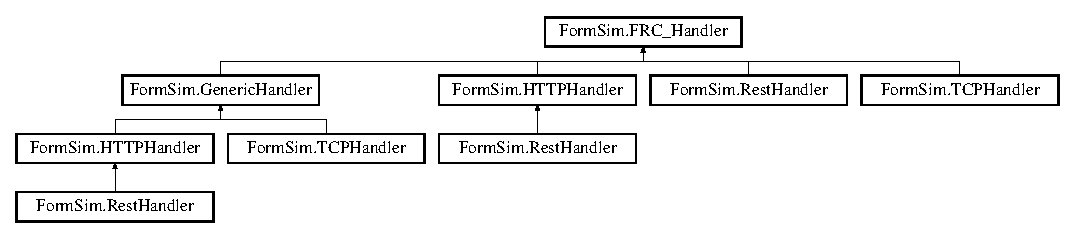
\includegraphics[height=2.748466cm]{interface_form_sim_1_1_f_r_c___handler}
\end{center}
\end{figure}
\subsection*{Public Member Functions}
\begin{DoxyCompactItemize}
\item 
Task$<$ bool $>$ \mbox{\hyperlink{interface_form_sim_1_1_f_r_c___handler_a32c299d3cb3cdd6c444e76b3671af1b4}{perform\+Token\+Exchange}} ()
\begin{DoxyCompactList}\small\item\em Performs the token exchange with the client\+G\+U\+ID and Auth Token in exchange for an access token. N\+O\+TE\+: Both the client\+G\+U\+ID and the Auth\+Token must have been previously set or token exchange will fail. See \mbox{\hyperlink{interface_form_sim_1_1_f_r_c___handler_a3c77b2e99c98553928e463a9cbb5f7d4}{set\+Client\+G\+U\+I\+D(string)}} A\+ND See \mbox{\hyperlink{interface_form_sim_1_1_f_r_c___handler_a1314ea0937067435e3326818baa9d0c1}{set\+Auth\+Token(string)}} \end{DoxyCompactList}\item 
Task$<$ Dictionary$<$ string, string $>$ $>$ \mbox{\hyperlink{interface_form_sim_1_1_f_r_c___handler_a2a2a8a776e774e5f8b5e2b7e623a26a6}{start}} (Dictionary$<$ string, string $>$ parameters)
\begin{DoxyCompactList}\small\item\em This provides the main entry point for the performing of a function based on the function request code that is passed in {\itshape parameters} . It automatically adjusts requestor references, sets a global timer for each function (for timeouts), and performs automatic voids and lookups based on the \char`\"{}\+Basic Transaction Flow\char`\"{} diagram found in the A\+PI Integrations guide. (Ver. 2.\+34, Pub. 6/6/18) \end{DoxyCompactList}\item 
Task$<$ Dictionary$<$ string, string $>$ $>$ \mbox{\hyperlink{interface_form_sim_1_1_f_r_c___handler_a1f855ed4026632d00ac5fc6784c3bf0f}{send\+Raw}} (string raw\+String)
\begin{DoxyCompactList}\small\item\em Sends a raw request to Shift4 for processing. This is mainly used as a debugging tool, to figure out if there are issues with the request, that can be deciphered ahead of hitting the Shift4 processing engine on the back side. This likely should be run in debug mode when full source is available as common errors that get thrown are not very descriptive. As time permits the error catching should be improved to hopefully throw more useful information about the actual error. \end{DoxyCompactList}\item 
Task$<$ Dictionary$<$ string, string $>$ $>$ \mbox{\hyperlink{interface_form_sim_1_1_f_r_c___handler_ad4b9146b6142d1d6ded15e5de4ed4675}{send\+Raw}} (string raw\+String, Dictionary$<$ string, string $>$ parameters)
\begin{DoxyCompactList}\small\item\em Overload Sends a raw request to Shift4 for processing. This is mainly used as a debugging tool, to figure out if there are issues with the request, that can be deciphered ahead of hitting the Shift4 processing engine on the back side. This likely should be run in debug mode when full source is available as common errors that get thrown are not very descriptive. As time permits the error catching should be improved to hopefully throw more useful information about the actual error. \end{DoxyCompactList}\item 
void \mbox{\hyperlink{interface_form_sim_1_1_f_r_c___handler_a702c2593fce6995a49f0fb509a2c7605}{set\+I\+P\+Address}} (string address)
\begin{DoxyCompactList}\small\item\em Sets the IP Address for which the U\+TG / Direct Post endpoint is located. \end{DoxyCompactList}\item 
string \mbox{\hyperlink{interface_form_sim_1_1_f_r_c___handler_ab4c19dd9eb34e0375b8a436fd01b79d0}{get\+I\+P\+Address}} ()
\begin{DoxyCompactList}\small\item\em Gets the IP Address \end{DoxyCompactList}\item 
void \mbox{\hyperlink{interface_form_sim_1_1_f_r_c___handler_a0a0a83b20fd2b3ec4ef9bbe5f5549b35}{set\+Port}} (string port)
\begin{DoxyCompactList}\small\item\em Sets the Port to connect to. N\+O\+TE\+: The use of the Port number only applies when the IP Address is not of the http form. \end{DoxyCompactList}\item 
string \mbox{\hyperlink{interface_form_sim_1_1_f_r_c___handler_add0725551d06bb4cfb33c23bef426814}{get\+Port}} ()
\begin{DoxyCompactList}\small\item\em Gets the Current Port Number \end{DoxyCompactList}\item 
void \mbox{\hyperlink{interface_form_sim_1_1_f_r_c___handler_a3c77b2e99c98553928e463a9cbb5f7d4}{set\+Client\+G\+U\+ID}} (string id)
\begin{DoxyCompactList}\small\item\em Sets the client G\+U\+ID. This really should not change for production uses, but for a sim it can be changed. \end{DoxyCompactList}\item 
string \mbox{\hyperlink{interface_form_sim_1_1_f_r_c___handler_a66f72d339aebc7c5b434026953a79044}{get\+Client\+G\+U\+ID}} ()
\begin{DoxyCompactList}\small\item\em Gets the current client\+G\+U\+ID. This really should not change for production uses, but for a sim it can be changed. \end{DoxyCompactList}\item 
void \mbox{\hyperlink{interface_form_sim_1_1_f_r_c___handler_a1314ea0937067435e3326818baa9d0c1}{set\+Auth\+Token}} (string token)
\begin{DoxyCompactList}\small\item\em Sets the Auth token that was provided by Shift4. This token needs to be able to be changed in production, so it should not be hard coded like the client\+G\+U\+ID should be. \end{DoxyCompactList}\item 
string \mbox{\hyperlink{interface_form_sim_1_1_f_r_c___handler_aeebaee9e36c649daae23db9fc710b261}{get\+Auth\+Token}} ()
\begin{DoxyCompactList}\small\item\em Gets the currently set Auth\+Token \end{DoxyCompactList}\item 
void \mbox{\hyperlink{interface_form_sim_1_1_f_r_c___handler_a6a11b11aaf8b033b87de9fddaf2d325e}{set\+Access\+Token}} (string token)
\begin{DoxyCompactList}\small\item\em Sets the Access\+Token. This token is sent in every request and is acquired by perfroming a token exchange. \mbox{\hyperlink{interface_form_sim_1_1_f_r_c___handler_a32c299d3cb3cdd6c444e76b3671af1b4}{perform\+Token\+Exchange()}} Failure to get an Access\+Token will result in refused transactions to Shift4. \end{DoxyCompactList}\item 
string \mbox{\hyperlink{interface_form_sim_1_1_f_r_c___handler_ad24521be35d127e83221c3c7ecf6fbf8}{get\+Access\+Token}} ()
\begin{DoxyCompactList}\small\item\em Gets the Access Token \end{DoxyCompactList}\item 
void \mbox{\hyperlink{interface_form_sim_1_1_f_r_c___handler_a23a2917fb9455954723cd3982b31b76c}{set\+Merchant\+Type}} (string type)
\begin{DoxyCompactList}\small\item\em Sets the Merchant Type. In a production environment this is likely already preselected based on their industry, however for a sim it is helpful in managing what fields get sent to the engine. For example, sending the expected length of a hotel stay for a food and beverage vendor does not make sense. Thus setting this to the right values, will prevent unnecessary parameters being passed to the engine. \end{DoxyCompactList}\item 
string \mbox{\hyperlink{interface_form_sim_1_1_f_r_c___handler_ad7484e0f6199cfae3beb33d91d6f1368}{get\+Merchant\+Type}} ()
\begin{DoxyCompactList}\small\item\em Gets the Industry Type of the current Merchant \end{DoxyCompactList}\end{DoxyCompactItemize}


\subsection{Member Function Documentation}
\mbox{\Hypertarget{interface_form_sim_1_1_f_r_c___handler_ad24521be35d127e83221c3c7ecf6fbf8}\label{interface_form_sim_1_1_f_r_c___handler_ad24521be35d127e83221c3c7ecf6fbf8}} 
\index{Form\+Sim\+::\+F\+R\+C\+\_\+\+Handler@{Form\+Sim\+::\+F\+R\+C\+\_\+\+Handler}!get\+Access\+Token@{get\+Access\+Token}}
\index{get\+Access\+Token@{get\+Access\+Token}!Form\+Sim\+::\+F\+R\+C\+\_\+\+Handler@{Form\+Sim\+::\+F\+R\+C\+\_\+\+Handler}}
\subsubsection{\texorpdfstring{get\+Access\+Token()}{getAccessToken()}}
{\footnotesize\ttfamily string Form\+Sim.\+F\+R\+C\+\_\+\+Handler.\+get\+Access\+Token (\begin{DoxyParamCaption}{ }\end{DoxyParamCaption})}



Gets the Access Token 

\begin{DoxyReturn}{Returns}
The Access Token
\end{DoxyReturn}


Implemented in \mbox{\hyperlink{class_form_sim_1_1_generic_handler_a220e1a96282940bc7b2fe8d898aec987}{Form\+Sim.\+Generic\+Handler}}.

\mbox{\Hypertarget{interface_form_sim_1_1_f_r_c___handler_aeebaee9e36c649daae23db9fc710b261}\label{interface_form_sim_1_1_f_r_c___handler_aeebaee9e36c649daae23db9fc710b261}} 
\index{Form\+Sim\+::\+F\+R\+C\+\_\+\+Handler@{Form\+Sim\+::\+F\+R\+C\+\_\+\+Handler}!get\+Auth\+Token@{get\+Auth\+Token}}
\index{get\+Auth\+Token@{get\+Auth\+Token}!Form\+Sim\+::\+F\+R\+C\+\_\+\+Handler@{Form\+Sim\+::\+F\+R\+C\+\_\+\+Handler}}
\subsubsection{\texorpdfstring{get\+Auth\+Token()}{getAuthToken()}}
{\footnotesize\ttfamily string Form\+Sim.\+F\+R\+C\+\_\+\+Handler.\+get\+Auth\+Token (\begin{DoxyParamCaption}{ }\end{DoxyParamCaption})}



Gets the currently set Auth\+Token 

\begin{DoxyReturn}{Returns}
The Auth\+Token
\end{DoxyReturn}


Implemented in \mbox{\hyperlink{class_form_sim_1_1_generic_handler_a4854fdfe77d09a6d2af723d2811099f5}{Form\+Sim.\+Generic\+Handler}}.

\mbox{\Hypertarget{interface_form_sim_1_1_f_r_c___handler_a66f72d339aebc7c5b434026953a79044}\label{interface_form_sim_1_1_f_r_c___handler_a66f72d339aebc7c5b434026953a79044}} 
\index{Form\+Sim\+::\+F\+R\+C\+\_\+\+Handler@{Form\+Sim\+::\+F\+R\+C\+\_\+\+Handler}!get\+Client\+G\+U\+ID@{get\+Client\+G\+U\+ID}}
\index{get\+Client\+G\+U\+ID@{get\+Client\+G\+U\+ID}!Form\+Sim\+::\+F\+R\+C\+\_\+\+Handler@{Form\+Sim\+::\+F\+R\+C\+\_\+\+Handler}}
\subsubsection{\texorpdfstring{get\+Client\+G\+U\+I\+D()}{getClientGUID()}}
{\footnotesize\ttfamily string Form\+Sim.\+F\+R\+C\+\_\+\+Handler.\+get\+Client\+G\+U\+ID (\begin{DoxyParamCaption}{ }\end{DoxyParamCaption})}



Gets the current client\+G\+U\+ID. This really should not change for production uses, but for a sim it can be changed. 

\begin{DoxyReturn}{Returns}
the current client\+G\+U\+ID
\end{DoxyReturn}


Implemented in \mbox{\hyperlink{class_form_sim_1_1_generic_handler_a16fe6657ef9d508f46dae9c8883a3a07}{Form\+Sim.\+Generic\+Handler}}.

\mbox{\Hypertarget{interface_form_sim_1_1_f_r_c___handler_ab4c19dd9eb34e0375b8a436fd01b79d0}\label{interface_form_sim_1_1_f_r_c___handler_ab4c19dd9eb34e0375b8a436fd01b79d0}} 
\index{Form\+Sim\+::\+F\+R\+C\+\_\+\+Handler@{Form\+Sim\+::\+F\+R\+C\+\_\+\+Handler}!get\+I\+P\+Address@{get\+I\+P\+Address}}
\index{get\+I\+P\+Address@{get\+I\+P\+Address}!Form\+Sim\+::\+F\+R\+C\+\_\+\+Handler@{Form\+Sim\+::\+F\+R\+C\+\_\+\+Handler}}
\subsubsection{\texorpdfstring{get\+I\+P\+Address()}{getIPAddress()}}
{\footnotesize\ttfamily string Form\+Sim.\+F\+R\+C\+\_\+\+Handler.\+get\+I\+P\+Address (\begin{DoxyParamCaption}{ }\end{DoxyParamCaption})}



Gets the IP Address 

\begin{DoxyReturn}{Returns}
The string representation of the IP Address
\end{DoxyReturn}


Implemented in \mbox{\hyperlink{class_form_sim_1_1_generic_handler_ab567abdefd58e1fcb3006861c741961c}{Form\+Sim.\+Generic\+Handler}}.

\mbox{\Hypertarget{interface_form_sim_1_1_f_r_c___handler_ad7484e0f6199cfae3beb33d91d6f1368}\label{interface_form_sim_1_1_f_r_c___handler_ad7484e0f6199cfae3beb33d91d6f1368}} 
\index{Form\+Sim\+::\+F\+R\+C\+\_\+\+Handler@{Form\+Sim\+::\+F\+R\+C\+\_\+\+Handler}!get\+Merchant\+Type@{get\+Merchant\+Type}}
\index{get\+Merchant\+Type@{get\+Merchant\+Type}!Form\+Sim\+::\+F\+R\+C\+\_\+\+Handler@{Form\+Sim\+::\+F\+R\+C\+\_\+\+Handler}}
\subsubsection{\texorpdfstring{get\+Merchant\+Type()}{getMerchantType()}}
{\footnotesize\ttfamily string Form\+Sim.\+F\+R\+C\+\_\+\+Handler.\+get\+Merchant\+Type (\begin{DoxyParamCaption}{ }\end{DoxyParamCaption})}



Gets the Industry Type of the current Merchant 

\begin{DoxyReturn}{Returns}
Industry Type of Merchant
\end{DoxyReturn}


Implemented in \mbox{\hyperlink{class_form_sim_1_1_generic_handler_a9bef42bcd6992d96947612aaab8f88a7}{Form\+Sim.\+Generic\+Handler}}.

\mbox{\Hypertarget{interface_form_sim_1_1_f_r_c___handler_add0725551d06bb4cfb33c23bef426814}\label{interface_form_sim_1_1_f_r_c___handler_add0725551d06bb4cfb33c23bef426814}} 
\index{Form\+Sim\+::\+F\+R\+C\+\_\+\+Handler@{Form\+Sim\+::\+F\+R\+C\+\_\+\+Handler}!get\+Port@{get\+Port}}
\index{get\+Port@{get\+Port}!Form\+Sim\+::\+F\+R\+C\+\_\+\+Handler@{Form\+Sim\+::\+F\+R\+C\+\_\+\+Handler}}
\subsubsection{\texorpdfstring{get\+Port()}{getPort()}}
{\footnotesize\ttfamily string Form\+Sim.\+F\+R\+C\+\_\+\+Handler.\+get\+Port (\begin{DoxyParamCaption}{ }\end{DoxyParamCaption})}



Gets the Current Port Number 

\begin{DoxyReturn}{Returns}
String Representation of the current port
\end{DoxyReturn}


Implemented in \mbox{\hyperlink{class_form_sim_1_1_generic_handler_a0e6f8152a789ba9f82501d45b029de71}{Form\+Sim.\+Generic\+Handler}}.

\mbox{\Hypertarget{interface_form_sim_1_1_f_r_c___handler_a32c299d3cb3cdd6c444e76b3671af1b4}\label{interface_form_sim_1_1_f_r_c___handler_a32c299d3cb3cdd6c444e76b3671af1b4}} 
\index{Form\+Sim\+::\+F\+R\+C\+\_\+\+Handler@{Form\+Sim\+::\+F\+R\+C\+\_\+\+Handler}!perform\+Token\+Exchange@{perform\+Token\+Exchange}}
\index{perform\+Token\+Exchange@{perform\+Token\+Exchange}!Form\+Sim\+::\+F\+R\+C\+\_\+\+Handler@{Form\+Sim\+::\+F\+R\+C\+\_\+\+Handler}}
\subsubsection{\texorpdfstring{perform\+Token\+Exchange()}{performTokenExchange()}}
{\footnotesize\ttfamily Task$<$bool$>$ Form\+Sim.\+F\+R\+C\+\_\+\+Handler.\+perform\+Token\+Exchange (\begin{DoxyParamCaption}{ }\end{DoxyParamCaption})}



Performs the token exchange with the client\+G\+U\+ID and Auth Token in exchange for an access token. N\+O\+TE\+: Both the client\+G\+U\+ID and the Auth\+Token must have been previously set or token exchange will fail. See \mbox{\hyperlink{interface_form_sim_1_1_f_r_c___handler_a3c77b2e99c98553928e463a9cbb5f7d4}{set\+Client\+G\+U\+I\+D(string)}} A\+ND See \mbox{\hyperlink{interface_form_sim_1_1_f_r_c___handler_a1314ea0937067435e3326818baa9d0c1}{set\+Auth\+Token(string)}} 

\begin{DoxyReturn}{Returns}
True if an Access token was received and set, false otherwise
\end{DoxyReturn}


Implemented in \mbox{\hyperlink{class_form_sim_1_1_rest_handler_abd5c425be2b6c9e30ca3cfc0fb696aa9}{Form\+Sim.\+Rest\+Handler}}, \mbox{\hyperlink{class_form_sim_1_1_generic_handler_a731bd7dada7e2d13fd9c9d768bd387ee}{Form\+Sim.\+Generic\+Handler}}, \mbox{\hyperlink{class_form_sim_1_1_t_c_p_handler_a61075c8a24b97ae7c86d357d6ee5a49e}{Form\+Sim.\+T\+C\+P\+Handler}}, and \mbox{\hyperlink{class_form_sim_1_1_h_t_t_p_handler_ae2ace13d7dc63f0bf1e1ef1a41bf8a3e}{Form\+Sim.\+H\+T\+T\+P\+Handler}}.

\mbox{\Hypertarget{interface_form_sim_1_1_f_r_c___handler_a1f855ed4026632d00ac5fc6784c3bf0f}\label{interface_form_sim_1_1_f_r_c___handler_a1f855ed4026632d00ac5fc6784c3bf0f}} 
\index{Form\+Sim\+::\+F\+R\+C\+\_\+\+Handler@{Form\+Sim\+::\+F\+R\+C\+\_\+\+Handler}!send\+Raw@{send\+Raw}}
\index{send\+Raw@{send\+Raw}!Form\+Sim\+::\+F\+R\+C\+\_\+\+Handler@{Form\+Sim\+::\+F\+R\+C\+\_\+\+Handler}}
\subsubsection{\texorpdfstring{send\+Raw()}{sendRaw()}\hspace{0.1cm}{\footnotesize\ttfamily [1/2]}}
{\footnotesize\ttfamily Task$<$Dictionary$<$string, string$>$ $>$ Form\+Sim.\+F\+R\+C\+\_\+\+Handler.\+send\+Raw (\begin{DoxyParamCaption}\item[{string}]{raw\+String }\end{DoxyParamCaption})}



Sends a raw request to Shift4 for processing. This is mainly used as a debugging tool, to figure out if there are issues with the request, that can be deciphered ahead of hitting the Shift4 processing engine on the back side. This likely should be run in debug mode when full source is available as common errors that get thrown are not very descriptive. As time permits the error catching should be improved to hopefully throw more useful information about the actual error. 


\begin{DoxyParams}{Parameters}
{\em raw\+String} & The Raw String to be sent\\
\hline
\end{DoxyParams}
\begin{DoxyReturn}{Returns}
A Dictionary of the returned parameters of the last function called. See N\+O\+TE at\+: \mbox{\hyperlink{interface_form_sim_1_1_f_r_c___handler_a2a2a8a776e774e5f8b5e2b7e623a26a6}{start(\+Dictionary$<$string, string$>$)}} as this note also applies here.
\end{DoxyReturn}


Implemented in \mbox{\hyperlink{class_form_sim_1_1_t_c_p_handler_a810309bc6e943b6ff12ebed8401613f0}{Form\+Sim.\+T\+C\+P\+Handler}}, \mbox{\hyperlink{class_form_sim_1_1_h_t_t_p_handler_a31006e646afd7cb331784dce27760d5b}{Form\+Sim.\+H\+T\+T\+P\+Handler}}, and \mbox{\hyperlink{class_form_sim_1_1_generic_handler_a806d781f9ad046f8f1574b137ffe86e0}{Form\+Sim.\+Generic\+Handler}}.

\mbox{\Hypertarget{interface_form_sim_1_1_f_r_c___handler_ad4b9146b6142d1d6ded15e5de4ed4675}\label{interface_form_sim_1_1_f_r_c___handler_ad4b9146b6142d1d6ded15e5de4ed4675}} 
\index{Form\+Sim\+::\+F\+R\+C\+\_\+\+Handler@{Form\+Sim\+::\+F\+R\+C\+\_\+\+Handler}!send\+Raw@{send\+Raw}}
\index{send\+Raw@{send\+Raw}!Form\+Sim\+::\+F\+R\+C\+\_\+\+Handler@{Form\+Sim\+::\+F\+R\+C\+\_\+\+Handler}}
\subsubsection{\texorpdfstring{send\+Raw()}{sendRaw()}\hspace{0.1cm}{\footnotesize\ttfamily [2/2]}}
{\footnotesize\ttfamily Task$<$Dictionary$<$string, string$>$ $>$ Form\+Sim.\+F\+R\+C\+\_\+\+Handler.\+send\+Raw (\begin{DoxyParamCaption}\item[{string}]{raw\+String,  }\item[{Dictionary$<$ string, string $>$}]{parameters }\end{DoxyParamCaption})}



Overload Sends a raw request to Shift4 for processing. This is mainly used as a debugging tool, to figure out if there are issues with the request, that can be deciphered ahead of hitting the Shift4 processing engine on the back side. This likely should be run in debug mode when full source is available as common errors that get thrown are not very descriptive. As time permits the error catching should be improved to hopefully throw more useful information about the actual error. 


\begin{DoxyParams}{Parameters}
{\em raw\+String} & The raw string to be sent\\
\hline
{\em parameters} & A list of parameters from the front end\\
\hline
\end{DoxyParams}
\begin{DoxyReturn}{Returns}

\end{DoxyReturn}


Implemented in \mbox{\hyperlink{class_form_sim_1_1_rest_handler_a4a777189e9e16dc9970fe8f2557555db}{Form\+Sim.\+Rest\+Handler}}, and \mbox{\hyperlink{class_form_sim_1_1_generic_handler_a9e6731b583644ba3bd5bde94ef86c678}{Form\+Sim.\+Generic\+Handler}}.

\mbox{\Hypertarget{interface_form_sim_1_1_f_r_c___handler_a6a11b11aaf8b033b87de9fddaf2d325e}\label{interface_form_sim_1_1_f_r_c___handler_a6a11b11aaf8b033b87de9fddaf2d325e}} 
\index{Form\+Sim\+::\+F\+R\+C\+\_\+\+Handler@{Form\+Sim\+::\+F\+R\+C\+\_\+\+Handler}!set\+Access\+Token@{set\+Access\+Token}}
\index{set\+Access\+Token@{set\+Access\+Token}!Form\+Sim\+::\+F\+R\+C\+\_\+\+Handler@{Form\+Sim\+::\+F\+R\+C\+\_\+\+Handler}}
\subsubsection{\texorpdfstring{set\+Access\+Token()}{setAccessToken()}}
{\footnotesize\ttfamily void Form\+Sim.\+F\+R\+C\+\_\+\+Handler.\+set\+Access\+Token (\begin{DoxyParamCaption}\item[{string}]{token }\end{DoxyParamCaption})}



Sets the Access\+Token. This token is sent in every request and is acquired by perfroming a token exchange. \mbox{\hyperlink{interface_form_sim_1_1_f_r_c___handler_a32c299d3cb3cdd6c444e76b3671af1b4}{perform\+Token\+Exchange()}} Failure to get an Access\+Token will result in refused transactions to Shift4. 


\begin{DoxyParams}{Parameters}
{\em token} & The Access Token\\
\hline
\end{DoxyParams}


Implemented in \mbox{\hyperlink{class_form_sim_1_1_generic_handler_ac2fe26607f27b8009b3d744bee7ba794}{Form\+Sim.\+Generic\+Handler}}.

\mbox{\Hypertarget{interface_form_sim_1_1_f_r_c___handler_a1314ea0937067435e3326818baa9d0c1}\label{interface_form_sim_1_1_f_r_c___handler_a1314ea0937067435e3326818baa9d0c1}} 
\index{Form\+Sim\+::\+F\+R\+C\+\_\+\+Handler@{Form\+Sim\+::\+F\+R\+C\+\_\+\+Handler}!set\+Auth\+Token@{set\+Auth\+Token}}
\index{set\+Auth\+Token@{set\+Auth\+Token}!Form\+Sim\+::\+F\+R\+C\+\_\+\+Handler@{Form\+Sim\+::\+F\+R\+C\+\_\+\+Handler}}
\subsubsection{\texorpdfstring{set\+Auth\+Token()}{setAuthToken()}}
{\footnotesize\ttfamily void Form\+Sim.\+F\+R\+C\+\_\+\+Handler.\+set\+Auth\+Token (\begin{DoxyParamCaption}\item[{string}]{token }\end{DoxyParamCaption})}



Sets the Auth token that was provided by Shift4. This token needs to be able to be changed in production, so it should not be hard coded like the client\+G\+U\+ID should be. 


\begin{DoxyParams}{Parameters}
{\em token} & The Auth\+Token for a particular mid\\
\hline
\end{DoxyParams}


Implemented in \mbox{\hyperlink{class_form_sim_1_1_generic_handler_a905d080f02134e993d7afbb1dcc8f44b}{Form\+Sim.\+Generic\+Handler}}.

\mbox{\Hypertarget{interface_form_sim_1_1_f_r_c___handler_a3c77b2e99c98553928e463a9cbb5f7d4}\label{interface_form_sim_1_1_f_r_c___handler_a3c77b2e99c98553928e463a9cbb5f7d4}} 
\index{Form\+Sim\+::\+F\+R\+C\+\_\+\+Handler@{Form\+Sim\+::\+F\+R\+C\+\_\+\+Handler}!set\+Client\+G\+U\+ID@{set\+Client\+G\+U\+ID}}
\index{set\+Client\+G\+U\+ID@{set\+Client\+G\+U\+ID}!Form\+Sim\+::\+F\+R\+C\+\_\+\+Handler@{Form\+Sim\+::\+F\+R\+C\+\_\+\+Handler}}
\subsubsection{\texorpdfstring{set\+Client\+G\+U\+I\+D()}{setClientGUID()}}
{\footnotesize\ttfamily void Form\+Sim.\+F\+R\+C\+\_\+\+Handler.\+set\+Client\+G\+U\+ID (\begin{DoxyParamCaption}\item[{string}]{id }\end{DoxyParamCaption})}



Sets the client G\+U\+ID. This really should not change for production uses, but for a sim it can be changed. 


\begin{DoxyParams}{Parameters}
{\em id} & client\+G\+U\+ID provided by Shift4\\
\hline
\end{DoxyParams}


Implemented in \mbox{\hyperlink{class_form_sim_1_1_generic_handler_a3c934d9ba3f0efaadac331502ce0189c}{Form\+Sim.\+Generic\+Handler}}.

\mbox{\Hypertarget{interface_form_sim_1_1_f_r_c___handler_a702c2593fce6995a49f0fb509a2c7605}\label{interface_form_sim_1_1_f_r_c___handler_a702c2593fce6995a49f0fb509a2c7605}} 
\index{Form\+Sim\+::\+F\+R\+C\+\_\+\+Handler@{Form\+Sim\+::\+F\+R\+C\+\_\+\+Handler}!set\+I\+P\+Address@{set\+I\+P\+Address}}
\index{set\+I\+P\+Address@{set\+I\+P\+Address}!Form\+Sim\+::\+F\+R\+C\+\_\+\+Handler@{Form\+Sim\+::\+F\+R\+C\+\_\+\+Handler}}
\subsubsection{\texorpdfstring{set\+I\+P\+Address()}{setIPAddress()}}
{\footnotesize\ttfamily void Form\+Sim.\+F\+R\+C\+\_\+\+Handler.\+set\+I\+P\+Address (\begin{DoxyParamCaption}\item[{string}]{address }\end{DoxyParamCaption})}



Sets the IP Address for which the U\+TG / Direct Post endpoint is located. 


\begin{DoxyParams}{Parameters}
{\em address} & The IP address of the U\+TG, \\
\hline
\end{DoxyParams}
or

The web address of the direct post endpoint$<$example$>$\href{https://www.shift4test.com}{\tt https\+://www.\+shift4test.\+com}

Implemented in \mbox{\hyperlink{class_form_sim_1_1_generic_handler_a7fa7f097410ae531b30fc6f257bcb393}{Form\+Sim.\+Generic\+Handler}}.

\mbox{\Hypertarget{interface_form_sim_1_1_f_r_c___handler_a23a2917fb9455954723cd3982b31b76c}\label{interface_form_sim_1_1_f_r_c___handler_a23a2917fb9455954723cd3982b31b76c}} 
\index{Form\+Sim\+::\+F\+R\+C\+\_\+\+Handler@{Form\+Sim\+::\+F\+R\+C\+\_\+\+Handler}!set\+Merchant\+Type@{set\+Merchant\+Type}}
\index{set\+Merchant\+Type@{set\+Merchant\+Type}!Form\+Sim\+::\+F\+R\+C\+\_\+\+Handler@{Form\+Sim\+::\+F\+R\+C\+\_\+\+Handler}}
\subsubsection{\texorpdfstring{set\+Merchant\+Type()}{setMerchantType()}}
{\footnotesize\ttfamily void Form\+Sim.\+F\+R\+C\+\_\+\+Handler.\+set\+Merchant\+Type (\begin{DoxyParamCaption}\item[{string}]{type }\end{DoxyParamCaption})}



Sets the Merchant Type. In a production environment this is likely already preselected based on their industry, however for a sim it is helpful in managing what fields get sent to the engine. For example, sending the expected length of a hotel stay for a food and beverage vendor does not make sense. Thus setting this to the right values, will prevent unnecessary parameters being passed to the engine. 


\begin{DoxyParams}{Parameters}
{\em type} & The Merchant Industry Type\\
\hline
\end{DoxyParams}


Implemented in \mbox{\hyperlink{class_form_sim_1_1_generic_handler_a0a3b84b949b002deecb5523cec3cae23}{Form\+Sim.\+Generic\+Handler}}.

\mbox{\Hypertarget{interface_form_sim_1_1_f_r_c___handler_a0a0a83b20fd2b3ec4ef9bbe5f5549b35}\label{interface_form_sim_1_1_f_r_c___handler_a0a0a83b20fd2b3ec4ef9bbe5f5549b35}} 
\index{Form\+Sim\+::\+F\+R\+C\+\_\+\+Handler@{Form\+Sim\+::\+F\+R\+C\+\_\+\+Handler}!set\+Port@{set\+Port}}
\index{set\+Port@{set\+Port}!Form\+Sim\+::\+F\+R\+C\+\_\+\+Handler@{Form\+Sim\+::\+F\+R\+C\+\_\+\+Handler}}
\subsubsection{\texorpdfstring{set\+Port()}{setPort()}}
{\footnotesize\ttfamily void Form\+Sim.\+F\+R\+C\+\_\+\+Handler.\+set\+Port (\begin{DoxyParamCaption}\item[{string}]{port }\end{DoxyParamCaption})}



Sets the Port to connect to. N\+O\+TE\+: The use of the Port number only applies when the IP Address is not of the http form. 


\begin{DoxyParams}{Parameters}
{\em port} & The port number\\
\hline
\end{DoxyParams}


Implemented in \mbox{\hyperlink{class_form_sim_1_1_generic_handler_ad22f25ee6f474e2ac46361add5ca7f97}{Form\+Sim.\+Generic\+Handler}}.

\mbox{\Hypertarget{interface_form_sim_1_1_f_r_c___handler_a2a2a8a776e774e5f8b5e2b7e623a26a6}\label{interface_form_sim_1_1_f_r_c___handler_a2a2a8a776e774e5f8b5e2b7e623a26a6}} 
\index{Form\+Sim\+::\+F\+R\+C\+\_\+\+Handler@{Form\+Sim\+::\+F\+R\+C\+\_\+\+Handler}!start@{start}}
\index{start@{start}!Form\+Sim\+::\+F\+R\+C\+\_\+\+Handler@{Form\+Sim\+::\+F\+R\+C\+\_\+\+Handler}}
\subsubsection{\texorpdfstring{start()}{start()}}
{\footnotesize\ttfamily Task$<$Dictionary$<$string, string$>$ $>$ Form\+Sim.\+F\+R\+C\+\_\+\+Handler.\+start (\begin{DoxyParamCaption}\item[{Dictionary$<$ string, string $>$}]{parameters }\end{DoxyParamCaption})}



This provides the main entry point for the performing of a function based on the function request code that is passed in {\itshape parameters} . It automatically adjusts requestor references, sets a global timer for each function (for timeouts), and performs automatic voids and lookups based on the \char`\"{}\+Basic Transaction Flow\char`\"{} diagram found in the A\+PI Integrations guide. (Ver. 2.\+34, Pub. 6/6/18) 


\begin{DoxyParams}{Parameters}
{\em parameters} & ~\newline
 {\bfseries Card\+Number} \+: Represents the unencrypted card number. This is often used when manual card entry is the method of choice. During voids, this number should be the last 4 of the card number, if a token is not available. In transactions where a card number is not being used, it should be blank.~\newline
 {\bfseries Expiration\+Date} \+: Represents the expiration date of the card. Expected for is M\+M\+YY. Note that no colons or slashes are used, as well as the date is of two digit format.~\newline
 {\bfseries C\+V\+V2} \+: This is the C\+V\+V2 value of the card, typically 3 or 4 digits.~\newline
 {\bfseries C\+V\+V2\+Indicator} \+: \char`\"{}1\char`\"{} if the C\+V\+V2 value is present in the parameter C\+V\+V2 above, \char`\"{}0\char`\"{} otherwise.~\newline
 {\bfseries Card\+Present} \+: \char`\"{}\+Y\char`\"{} if the card is present for the transaction, \char`\"{}\+N\char`\"{} if not. It may be necessary to leave this field blank when performing follow up transactions where this value was previously indicated.~\newline
 {\bfseries Street\+Address} \+: The billing street address.~\newline
 {\bfseries Destination\+Zip\+Code} \+: The location the item will be shipped to for mail order / telephone order (M\+O\+TO) or E-\/\+Commerce. For Retail, Lodging, and Auto, it should be the zip code of where the services are rendered, or goods are being sold from.~\newline
 {\bfseries Card\+Type} \+: N\+OT C\+U\+R\+R\+E\+N\+T\+LY U\+S\+ED -\/ leave blank~\newline
 {\bfseries Track\+Data} \+: Used for passing unencrypted Track Data when using a standard mag stripe reader (M\+SR).~\newline
 {\bfseries Unique\+ID} \+: Used to pass a token representing Card Holder Data (C\+HD), Required in True\+Token transactions.~\newline
 {\bfseries Token\+Serial} \+: Serial of the M\+ID. Should be used when using Token\+Sharing, or a Global Token Store.~\newline
 {\bfseries A\+P\+I\+Options} \+: A comma delimited list of A\+PI Options to be sent with the request.~\newline
 {\bfseries Invoice} \+: In invoice number of size not larger than 10 characters.~\newline
 {\bfseries Primary\+Amount} \+: The subtotal amount not including tax and or tip amounts. Note for T\+CP transactions omit the decimal point.~\newline
 {\bfseries Sale\+Flag} \+: \char`\"{}\+S\char`\"{} if performing a sale, and \char`\"{}\+C\char`\"{} if performing a refund.~\newline
 {\bfseries Zip\+Code} \+: The billing zip code.~\newline
 {\bfseries Secondary\+Amount} \+: The tip amount.~\newline
 {\bfseries Function\+Request\+Code} \+: The function request code desired to be performed.~\newline
 {\bfseries Tax\+Indicator} \+: \char`\"{}\+Y\char`\"{} if tax was charged, \char`\"{}\+N\char`\"{} otherwise.~\newline
 {\bfseries Tax\+Amount} \+: The Amount of Tax Charged. Note for T\+CP Transactions omit the decimal point.~\newline
 {\bfseries Tran\+ID} \+: The transaction ID sent back from a transaction. Used for rollbacks of failed incremental authorizations.~\newline
 {\bfseries Clerk} \+: Five digit clerk ID.~\newline
 {\bfseries Terminal\+ID} \+: The ID of the P\+IN pad set in U\+TG Tune-\/\+Up. Used to prompt and display to P\+IN Pad.~\newline
 {\bfseries Date} \+: Current Date in M\+M\+D\+D\+YY format.~\newline
 {\bfseries Time} \+: Current Time in H\+H\+M\+M\+SS format.~\newline
 {\bfseries Requestor\+Reference} \+: A refernece number for the request.~\newline
 {\bfseries P2\+P\+E\+Block} \+: The P2\+PE Block form a native P2\+PE device.~\newline
 {\bfseries Customer\+Name} \+: The name of the Customer.~\newline
 {\bfseries Void\+Invalid\+A\+VS} \+: A \char`\"{}\+Y\char`\"{} / \char`\"{}\+N\char`\"{} switch used to automatically void responses with invalid A\+VS responses.~\newline
 {\bfseries Void\+Invalid\+C\+V\+V2} \+: A \char`\"{}\+Y\char`\"{} / \char`\"{}\+N\char`\"{} switch used to automatically void responses with invalid C\+V\+V2 responses.~\newline
 {\bfseries Use\+Token\+Store} \+: A \char`\"{}\+Y\char`\"{} / \char`\"{}\+N\char`\"{} switch used to use a Token Store.~\newline
 {\bfseries Use\+Meta\+Token} \+: A \char`\"{}\+Y\char`\"{} / \char`\"{}\+N\char`\"{} switch used to use a Meta\+Token.~\newline
 {\bfseries Use\+Basic\+Tran\+Flow} \+: A \char`\"{}\+Y\char`\"{} / \char`\"{}\+N\char`\"{} switch used to control if the automaticity of the basic transaction flow is used when issuing function request codes. By turning this switch off, only single F\+R\+Cs will be executed regardlesss of the result that comes back from the server.~\newline
 {\bfseries Use\+Rollbacks} \+: A \char`\"{}\+Y\char`\"{} / \char`\"{}\+N\char`\"{} switch used to control if a void (F\+RC 08) will be used as a complete transaction void or if it will be used to roll back the transaction to it\textquotesingle{}s last approved state.~\newline
 \\
\hline
\end{DoxyParams}
\begin{DoxyReturn}{Returns}
A Dictionary of the returned parameters and results of the last function called. 

Note\+: In cases where automatic voids are called for, the response of the original request will N\+OT be retuned, but rather the result of the automatic void will be called. To see all of the transaction requests and responses, please check the log file that is generated.
\end{DoxyReturn}


Implemented in \mbox{\hyperlink{class_form_sim_1_1_generic_handler_affac9485687a2be1595405d657922532}{Form\+Sim.\+Generic\+Handler}}.



The documentation for this interface was generated from the following file\+:\begin{DoxyCompactItemize}
\item 
\mbox{\hyperlink{_f_r_c___handler_8cs}{F\+R\+C\+\_\+\+Handler.\+cs}}\end{DoxyCompactItemize}

\hypertarget{class_form_sim_1_1_generic_handler}{}\section{Form\+Sim.\+Generic\+Handler Class Reference}
\label{class_form_sim_1_1_generic_handler}\index{Form\+Sim.\+Generic\+Handler@{Form\+Sim.\+Generic\+Handler}}


The \mbox{\hyperlink{class_form_sim_1_1_generic_handler}{Generic\+Handler}} class is used as a super class for the more specific \mbox{\hyperlink{class_form_sim_1_1_h_t_t_p_handler}{H\+T\+T\+P\+Handler}} and the \mbox{\hyperlink{class_form_sim_1_1_t_c_p_handler}{T\+C\+P\+Handler}} classes which implement the protocol specific functionality. This class sets up the basic entry point for handling Function Request Codes (F\+R\+Cs) that should be implemented with the protocol specific handlers. By utilizing this entry point, Global timers are set up to check for time out occurences and customer references are maintained and tracked.  


Inheritance diagram for Form\+Sim.\+Generic\+Handler\+:\begin{figure}[H]
\begin{center}
\leavevmode
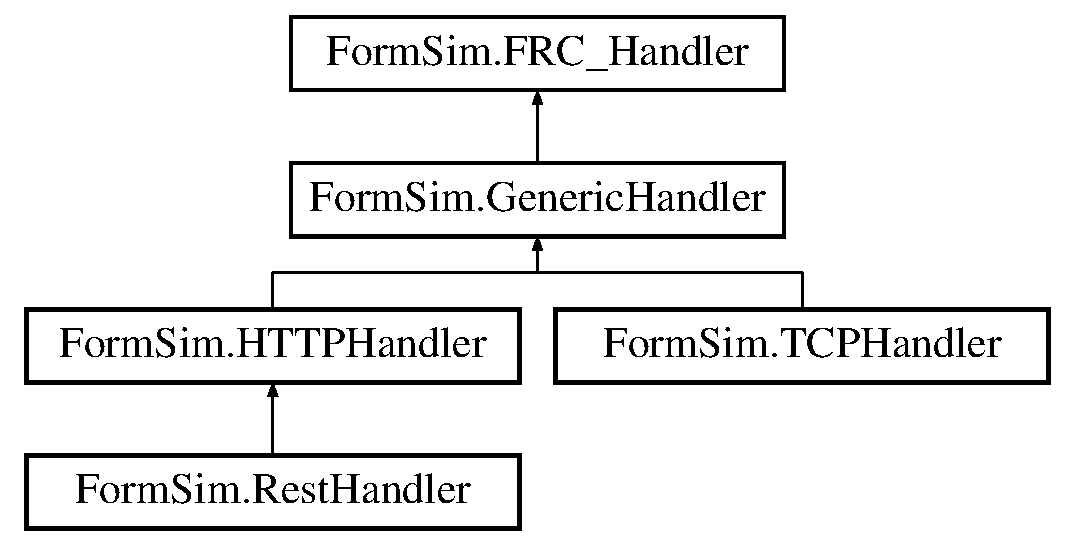
\includegraphics[height=4.000000cm]{class_form_sim_1_1_generic_handler}
\end{center}
\end{figure}
\subsection*{Public Member Functions}
\begin{DoxyCompactItemize}
\item 
\mbox{\hyperlink{class_form_sim_1_1_generic_handler_a49bc6036b85224e56603c6d9401456ef}{Generic\+Handler}} ()
\item 
\mbox{\hyperlink{class_form_sim_1_1_generic_handler_aa4beee84a911e42906528ea1d1ad6193}{Generic\+Handler}} (string \mbox{\hyperlink{class_form_sim_1_1_generic_handler_a6699d8bfc9cd305baf30ab9413b21605}{Auth\+Token}}, string \mbox{\hyperlink{class_form_sim_1_1_generic_handler_ae1d2175b140f4c600d74bbab1e22714e}{Client\+G\+U\+ID}})
\item 
\mbox{\hyperlink{class_form_sim_1_1_generic_handler_a39722a58046cfc8b36e3fde80ccc69f1}{Generic\+Handler}} (string \mbox{\hyperlink{class_form_sim_1_1_generic_handler_a6699d8bfc9cd305baf30ab9413b21605}{Auth\+Token}}, string \mbox{\hyperlink{class_form_sim_1_1_generic_handler_ae1d2175b140f4c600d74bbab1e22714e}{Client\+G\+U\+ID}}, string \mbox{\hyperlink{class_form_sim_1_1_generic_handler_a12b51dea082a4d40d86829802adf073b}{I\+P\+Address}}, string \mbox{\hyperlink{class_form_sim_1_1_generic_handler_ac6492bb3e4fbe8f66c97b00bd27020c1}{Port}})
\item 
virtual async Task$<$ bool $>$ \mbox{\hyperlink{class_form_sim_1_1_generic_handler_a731bd7dada7e2d13fd9c9d768bd387ee}{perform\+Token\+Exchange}} ()
\begin{DoxyCompactList}\small\item\em Performs the token exchange with the client\+G\+U\+ID and Auth Token in exchange for an access token. N\+O\+TE\+: Both the client\+G\+U\+ID and the Auth\+Token must have been previously set or token exchange will fail. See \mbox{\hyperlink{class_form_sim_1_1_generic_handler_a3c934d9ba3f0efaadac331502ce0189c}{set\+Client\+G\+U\+I\+D(string)}} A\+ND See \mbox{\hyperlink{class_form_sim_1_1_generic_handler_a905d080f02134e993d7afbb1dcc8f44b}{set\+Auth\+Token(string)}} \end{DoxyCompactList}\item 
async Task$<$ Dictionary$<$ string, string $>$ $>$ \mbox{\hyperlink{class_form_sim_1_1_generic_handler_affac9485687a2be1595405d657922532}{start}} (Dictionary$<$ string, string $>$ parameters)
\begin{DoxyCompactList}\small\item\em The primary entry point for executing F\+R\+Cs. \end{DoxyCompactList}\item 
virtual async Task$<$ Dictionary$<$ string, string $>$ $>$ \mbox{\hyperlink{class_form_sim_1_1_generic_handler_a806d781f9ad046f8f1574b137ffe86e0}{send\+Raw}} (string raw\+String)
\begin{DoxyCompactList}\small\item\em Sends a raw request to Shift4 for processing. This is mainly used as a debugging tool, to figure out if there are issues with the request, that can be deciphered ahead of hitting the Shift4 processing engine on the back side. This likely should be run in debug mode when full source is available as common errors that get thrown are not very descriptive. As time permits the error catching should be improved to hopefully throw more useful information about the actual error. \end{DoxyCompactList}\item 
virtual async Task$<$ Dictionary$<$ string, string $>$ $>$ \mbox{\hyperlink{class_form_sim_1_1_generic_handler_a9e6731b583644ba3bd5bde94ef86c678}{send\+Raw}} (string raw\+String, Dictionary$<$ string, string $>$ parameters)
\begin{DoxyCompactList}\small\item\em Overload Sends a raw request to Shift4 for processing. This is mainly used as a debugging tool, to figure out if there are issues with the request, that can be deciphered ahead of hitting the Shift4 processing engine on the back side. This likely should be run in debug mode when full source is available as common errors that get thrown are not very descriptive. As time permits the error catching should be improved to hopefully throw more useful information about the actual error. \end{DoxyCompactList}\item 
void \mbox{\hyperlink{class_form_sim_1_1_generic_handler_a7fa7f097410ae531b30fc6f257bcb393}{set\+I\+P\+Address}} (string address)
\begin{DoxyCompactList}\small\item\em Sets the IP Address for which the U\+TG / Direct Post endpoint is located. \end{DoxyCompactList}\item 
string \mbox{\hyperlink{class_form_sim_1_1_generic_handler_ab567abdefd58e1fcb3006861c741961c}{get\+I\+P\+Address}} ()
\begin{DoxyCompactList}\small\item\em Gets the IP Address \end{DoxyCompactList}\item 
void \mbox{\hyperlink{class_form_sim_1_1_generic_handler_ad22f25ee6f474e2ac46361add5ca7f97}{set\+Port}} (string \mbox{\hyperlink{class_form_sim_1_1_generic_handler_ac6492bb3e4fbe8f66c97b00bd27020c1}{Port}})
\begin{DoxyCompactList}\small\item\em Sets the Port to connect to. N\+O\+TE\+: The use of the Port number only applies when the IP Address is not of the http form. \end{DoxyCompactList}\item 
string \mbox{\hyperlink{class_form_sim_1_1_generic_handler_a0e6f8152a789ba9f82501d45b029de71}{get\+Port}} ()
\begin{DoxyCompactList}\small\item\em Gets the Current Port Number \end{DoxyCompactList}\item 
void \mbox{\hyperlink{class_form_sim_1_1_generic_handler_a3c934d9ba3f0efaadac331502ce0189c}{set\+Client\+G\+U\+ID}} (string id)
\begin{DoxyCompactList}\small\item\em Sets the client G\+U\+ID. This really should not change for production uses, but for a sim it can be changed. \end{DoxyCompactList}\item 
string \mbox{\hyperlink{class_form_sim_1_1_generic_handler_a16fe6657ef9d508f46dae9c8883a3a07}{get\+Client\+G\+U\+ID}} ()
\begin{DoxyCompactList}\small\item\em Gets the current client\+G\+U\+ID. This really should not change for production uses, but for a sim it can be changed. \end{DoxyCompactList}\item 
void \mbox{\hyperlink{class_form_sim_1_1_generic_handler_a905d080f02134e993d7afbb1dcc8f44b}{set\+Auth\+Token}} (string token)
\begin{DoxyCompactList}\small\item\em Sets the Auth token that was provided by Shift4. This token needs to be able to be changed in production, so it should not be hard coded like the client\+G\+U\+ID should be. \end{DoxyCompactList}\item 
string \mbox{\hyperlink{class_form_sim_1_1_generic_handler_a4854fdfe77d09a6d2af723d2811099f5}{get\+Auth\+Token}} ()
\begin{DoxyCompactList}\small\item\em Gets the currently set Auth\+Token \end{DoxyCompactList}\item 
void \mbox{\hyperlink{class_form_sim_1_1_generic_handler_ac2fe26607f27b8009b3d744bee7ba794}{set\+Access\+Token}} (string token)
\begin{DoxyCompactList}\small\item\em Sets the Access\+Token. This token is sent in every request and is acquired by perfroming a token exchange. \mbox{\hyperlink{class_form_sim_1_1_generic_handler_a731bd7dada7e2d13fd9c9d768bd387ee}{perform\+Token\+Exchange()}} Failure to get an Access\+Token will result in refused transactions to Shift4. \end{DoxyCompactList}\item 
string \mbox{\hyperlink{class_form_sim_1_1_generic_handler_a220e1a96282940bc7b2fe8d898aec987}{get\+Access\+Token}} ()
\begin{DoxyCompactList}\small\item\em Gets the Access Token \end{DoxyCompactList}\item 
void \mbox{\hyperlink{class_form_sim_1_1_generic_handler_a0a3b84b949b002deecb5523cec3cae23}{set\+Merchant\+Type}} (string type)
\begin{DoxyCompactList}\small\item\em Sets the Merchant Type. In a production environment this is likely already preselected based on their industry, however for a sim it is helpful in managing what fields get sent to the engine. For example, sending the expected length of a hotel stay for a food and beverage vendor does not make sense. Thus setting this to the right values, will prevent unnecessary parameters being passed to the engine. \end{DoxyCompactList}\item 
string \mbox{\hyperlink{class_form_sim_1_1_generic_handler_a9bef42bcd6992d96947612aaab8f88a7}{get\+Merchant\+Type}} ()
\begin{DoxyCompactList}\small\item\em Gets the Industry Type of the current Merchant \end{DoxyCompactList}\end{DoxyCompactItemize}
\subsection*{Protected Member Functions}
\begin{DoxyCompactItemize}
\item 
async Task$<$ Dictionary$<$ string, string $>$ $>$ \mbox{\hyperlink{class_form_sim_1_1_generic_handler_a8cb06afb7f6aed51488c7418491b9dd3}{start\+Transaction}} (Dictionary$<$ string, string $>$ parameters)
\begin{DoxyCompactList}\small\item\em Method that sets up the global timers needed to check for timeouts. This method is used internally and should not generally be used except in rare or specific cases. Use of \mbox{\hyperlink{class_form_sim_1_1_generic_handler_affac9485687a2be1595405d657922532}{start(\+Dictionary$<$string, string$>$)}} is advised for best results. \end{DoxyCompactList}\item 
virtual async Task$<$ Dictionary$<$ string, string $>$ $>$ \mbox{\hyperlink{class_form_sim_1_1_generic_handler_a824697e5c22a4f1cf8ce4e512b6954ad}{perform\+Transaction}} (Dictionary$<$ string, string $>$ parameters)
\begin{DoxyCompactList}\small\item\em This method needs to be Overridden by a subclass. Method exists here only to allow complete compilation. \end{DoxyCompactList}\end{DoxyCompactItemize}
\subsection*{Protected Attributes}
\begin{DoxyCompactItemize}
\item 
string \mbox{\hyperlink{class_form_sim_1_1_generic_handler_ae1d2175b140f4c600d74bbab1e22714e}{Client\+G\+U\+ID}}
\item 
string \mbox{\hyperlink{class_form_sim_1_1_generic_handler_a6699d8bfc9cd305baf30ab9413b21605}{Auth\+Token}}
\item 
string \mbox{\hyperlink{class_form_sim_1_1_generic_handler_ad47864be2c5790106a7538f640b2792f}{Access\+Token}}
\item 
string \mbox{\hyperlink{class_form_sim_1_1_generic_handler_a12b51dea082a4d40d86829802adf073b}{I\+P\+Address}}
\item 
string \mbox{\hyperlink{class_form_sim_1_1_generic_handler_ac6492bb3e4fbe8f66c97b00bd27020c1}{Port}}
\item 
\mbox{\hyperlink{class_form_sim_1_1_log_writer}{Log\+Writer}} \mbox{\hyperlink{class_form_sim_1_1_generic_handler_ad66bd80f77548cf730fa7b9bcffb3c0e}{log}} = \mbox{\hyperlink{class_form_sim_1_1_log_writer_ac885dc41c236f618e066cdcee8189f64}{Log\+Writer.\+get\+Instance}}
\item 
\mbox{\hyperlink{class_form_sim_1_1_helper}{Helper}} \mbox{\hyperlink{class_form_sim_1_1_generic_handler_a031b68c3e31ae8c99dc60a26d33f5de5}{helper}} = \mbox{\hyperlink{class_form_sim_1_1_helper_ac61d1dca7ce9b1fa7e4ce17e99b0b7e1}{Helper.\+get\+Instance}}
\item 
string \mbox{\hyperlink{class_form_sim_1_1_generic_handler_a8b7d568966660d7d3700eac963caa504}{Merchant\+Type}} = \char`\"{}Mo\+To\+Ecom\char`\"{}
\end{DoxyCompactItemize}


\subsection{Detailed Description}
The \mbox{\hyperlink{class_form_sim_1_1_generic_handler}{Generic\+Handler}} class is used as a super class for the more specific \mbox{\hyperlink{class_form_sim_1_1_h_t_t_p_handler}{H\+T\+T\+P\+Handler}} and the \mbox{\hyperlink{class_form_sim_1_1_t_c_p_handler}{T\+C\+P\+Handler}} classes which implement the protocol specific functionality. This class sets up the basic entry point for handling Function Request Codes (F\+R\+Cs) that should be implemented with the protocol specific handlers. By utilizing this entry point, Global timers are set up to check for time out occurences and customer references are maintained and tracked. 



\subsection{Constructor \& Destructor Documentation}
\mbox{\Hypertarget{class_form_sim_1_1_generic_handler_a49bc6036b85224e56603c6d9401456ef}\label{class_form_sim_1_1_generic_handler_a49bc6036b85224e56603c6d9401456ef}} 
\index{Form\+Sim\+::\+Generic\+Handler@{Form\+Sim\+::\+Generic\+Handler}!Generic\+Handler@{Generic\+Handler}}
\index{Generic\+Handler@{Generic\+Handler}!Form\+Sim\+::\+Generic\+Handler@{Form\+Sim\+::\+Generic\+Handler}}
\subsubsection{\texorpdfstring{Generic\+Handler()}{GenericHandler()}\hspace{0.1cm}{\footnotesize\ttfamily [1/3]}}
{\footnotesize\ttfamily Form\+Sim.\+Generic\+Handler.\+Generic\+Handler (\begin{DoxyParamCaption}{ }\end{DoxyParamCaption})\hspace{0.3cm}{\ttfamily [inline]}}

\mbox{\Hypertarget{class_form_sim_1_1_generic_handler_aa4beee84a911e42906528ea1d1ad6193}\label{class_form_sim_1_1_generic_handler_aa4beee84a911e42906528ea1d1ad6193}} 
\index{Form\+Sim\+::\+Generic\+Handler@{Form\+Sim\+::\+Generic\+Handler}!Generic\+Handler@{Generic\+Handler}}
\index{Generic\+Handler@{Generic\+Handler}!Form\+Sim\+::\+Generic\+Handler@{Form\+Sim\+::\+Generic\+Handler}}
\subsubsection{\texorpdfstring{Generic\+Handler()}{GenericHandler()}\hspace{0.1cm}{\footnotesize\ttfamily [2/3]}}
{\footnotesize\ttfamily Form\+Sim.\+Generic\+Handler.\+Generic\+Handler (\begin{DoxyParamCaption}\item[{string}]{Auth\+Token,  }\item[{string}]{Client\+G\+U\+ID }\end{DoxyParamCaption})\hspace{0.3cm}{\ttfamily [inline]}}

\mbox{\Hypertarget{class_form_sim_1_1_generic_handler_a39722a58046cfc8b36e3fde80ccc69f1}\label{class_form_sim_1_1_generic_handler_a39722a58046cfc8b36e3fde80ccc69f1}} 
\index{Form\+Sim\+::\+Generic\+Handler@{Form\+Sim\+::\+Generic\+Handler}!Generic\+Handler@{Generic\+Handler}}
\index{Generic\+Handler@{Generic\+Handler}!Form\+Sim\+::\+Generic\+Handler@{Form\+Sim\+::\+Generic\+Handler}}
\subsubsection{\texorpdfstring{Generic\+Handler()}{GenericHandler()}\hspace{0.1cm}{\footnotesize\ttfamily [3/3]}}
{\footnotesize\ttfamily Form\+Sim.\+Generic\+Handler.\+Generic\+Handler (\begin{DoxyParamCaption}\item[{string}]{Auth\+Token,  }\item[{string}]{Client\+G\+U\+ID,  }\item[{string}]{I\+P\+Address,  }\item[{string}]{Port }\end{DoxyParamCaption})\hspace{0.3cm}{\ttfamily [inline]}}



\subsection{Member Function Documentation}
\mbox{\Hypertarget{class_form_sim_1_1_generic_handler_a220e1a96282940bc7b2fe8d898aec987}\label{class_form_sim_1_1_generic_handler_a220e1a96282940bc7b2fe8d898aec987}} 
\index{Form\+Sim\+::\+Generic\+Handler@{Form\+Sim\+::\+Generic\+Handler}!get\+Access\+Token@{get\+Access\+Token}}
\index{get\+Access\+Token@{get\+Access\+Token}!Form\+Sim\+::\+Generic\+Handler@{Form\+Sim\+::\+Generic\+Handler}}
\subsubsection{\texorpdfstring{get\+Access\+Token()}{getAccessToken()}}
{\footnotesize\ttfamily string Form\+Sim.\+Generic\+Handler.\+get\+Access\+Token (\begin{DoxyParamCaption}{ }\end{DoxyParamCaption})\hspace{0.3cm}{\ttfamily [inline]}}



Gets the Access Token 

\begin{DoxyReturn}{Returns}
The Access Token
\end{DoxyReturn}


Implements \mbox{\hyperlink{interface_form_sim_1_1_f_r_c___handler_ad24521be35d127e83221c3c7ecf6fbf8}{Form\+Sim.\+F\+R\+C\+\_\+\+Handler}}.

\mbox{\Hypertarget{class_form_sim_1_1_generic_handler_a4854fdfe77d09a6d2af723d2811099f5}\label{class_form_sim_1_1_generic_handler_a4854fdfe77d09a6d2af723d2811099f5}} 
\index{Form\+Sim\+::\+Generic\+Handler@{Form\+Sim\+::\+Generic\+Handler}!get\+Auth\+Token@{get\+Auth\+Token}}
\index{get\+Auth\+Token@{get\+Auth\+Token}!Form\+Sim\+::\+Generic\+Handler@{Form\+Sim\+::\+Generic\+Handler}}
\subsubsection{\texorpdfstring{get\+Auth\+Token()}{getAuthToken()}}
{\footnotesize\ttfamily string Form\+Sim.\+Generic\+Handler.\+get\+Auth\+Token (\begin{DoxyParamCaption}{ }\end{DoxyParamCaption})\hspace{0.3cm}{\ttfamily [inline]}}



Gets the currently set Auth\+Token 

\begin{DoxyReturn}{Returns}
The Auth\+Token
\end{DoxyReturn}


Implements \mbox{\hyperlink{interface_form_sim_1_1_f_r_c___handler_aeebaee9e36c649daae23db9fc710b261}{Form\+Sim.\+F\+R\+C\+\_\+\+Handler}}.

\mbox{\Hypertarget{class_form_sim_1_1_generic_handler_a16fe6657ef9d508f46dae9c8883a3a07}\label{class_form_sim_1_1_generic_handler_a16fe6657ef9d508f46dae9c8883a3a07}} 
\index{Form\+Sim\+::\+Generic\+Handler@{Form\+Sim\+::\+Generic\+Handler}!get\+Client\+G\+U\+ID@{get\+Client\+G\+U\+ID}}
\index{get\+Client\+G\+U\+ID@{get\+Client\+G\+U\+ID}!Form\+Sim\+::\+Generic\+Handler@{Form\+Sim\+::\+Generic\+Handler}}
\subsubsection{\texorpdfstring{get\+Client\+G\+U\+I\+D()}{getClientGUID()}}
{\footnotesize\ttfamily string Form\+Sim.\+Generic\+Handler.\+get\+Client\+G\+U\+ID (\begin{DoxyParamCaption}{ }\end{DoxyParamCaption})\hspace{0.3cm}{\ttfamily [inline]}}



Gets the current client\+G\+U\+ID. This really should not change for production uses, but for a sim it can be changed. 

\begin{DoxyReturn}{Returns}
the current client\+G\+U\+ID
\end{DoxyReturn}


Implements \mbox{\hyperlink{interface_form_sim_1_1_f_r_c___handler_a66f72d339aebc7c5b434026953a79044}{Form\+Sim.\+F\+R\+C\+\_\+\+Handler}}.

\mbox{\Hypertarget{class_form_sim_1_1_generic_handler_ab567abdefd58e1fcb3006861c741961c}\label{class_form_sim_1_1_generic_handler_ab567abdefd58e1fcb3006861c741961c}} 
\index{Form\+Sim\+::\+Generic\+Handler@{Form\+Sim\+::\+Generic\+Handler}!get\+I\+P\+Address@{get\+I\+P\+Address}}
\index{get\+I\+P\+Address@{get\+I\+P\+Address}!Form\+Sim\+::\+Generic\+Handler@{Form\+Sim\+::\+Generic\+Handler}}
\subsubsection{\texorpdfstring{get\+I\+P\+Address()}{getIPAddress()}}
{\footnotesize\ttfamily string Form\+Sim.\+Generic\+Handler.\+get\+I\+P\+Address (\begin{DoxyParamCaption}{ }\end{DoxyParamCaption})\hspace{0.3cm}{\ttfamily [inline]}}



Gets the IP Address 

\begin{DoxyReturn}{Returns}
The string representation of the IP Address
\end{DoxyReturn}


Implements \mbox{\hyperlink{interface_form_sim_1_1_f_r_c___handler_ab4c19dd9eb34e0375b8a436fd01b79d0}{Form\+Sim.\+F\+R\+C\+\_\+\+Handler}}.

\mbox{\Hypertarget{class_form_sim_1_1_generic_handler_a9bef42bcd6992d96947612aaab8f88a7}\label{class_form_sim_1_1_generic_handler_a9bef42bcd6992d96947612aaab8f88a7}} 
\index{Form\+Sim\+::\+Generic\+Handler@{Form\+Sim\+::\+Generic\+Handler}!get\+Merchant\+Type@{get\+Merchant\+Type}}
\index{get\+Merchant\+Type@{get\+Merchant\+Type}!Form\+Sim\+::\+Generic\+Handler@{Form\+Sim\+::\+Generic\+Handler}}
\subsubsection{\texorpdfstring{get\+Merchant\+Type()}{getMerchantType()}}
{\footnotesize\ttfamily string Form\+Sim.\+Generic\+Handler.\+get\+Merchant\+Type (\begin{DoxyParamCaption}{ }\end{DoxyParamCaption})\hspace{0.3cm}{\ttfamily [inline]}}



Gets the Industry Type of the current Merchant 

\begin{DoxyReturn}{Returns}
Industry Type of Merchant
\end{DoxyReturn}


Implements \mbox{\hyperlink{interface_form_sim_1_1_f_r_c___handler_ad7484e0f6199cfae3beb33d91d6f1368}{Form\+Sim.\+F\+R\+C\+\_\+\+Handler}}.

\mbox{\Hypertarget{class_form_sim_1_1_generic_handler_a0e6f8152a789ba9f82501d45b029de71}\label{class_form_sim_1_1_generic_handler_a0e6f8152a789ba9f82501d45b029de71}} 
\index{Form\+Sim\+::\+Generic\+Handler@{Form\+Sim\+::\+Generic\+Handler}!get\+Port@{get\+Port}}
\index{get\+Port@{get\+Port}!Form\+Sim\+::\+Generic\+Handler@{Form\+Sim\+::\+Generic\+Handler}}
\subsubsection{\texorpdfstring{get\+Port()}{getPort()}}
{\footnotesize\ttfamily string Form\+Sim.\+Generic\+Handler.\+get\+Port (\begin{DoxyParamCaption}{ }\end{DoxyParamCaption})\hspace{0.3cm}{\ttfamily [inline]}}



Gets the Current Port Number 

\begin{DoxyReturn}{Returns}
String Representation of the current port
\end{DoxyReturn}


Implements \mbox{\hyperlink{interface_form_sim_1_1_f_r_c___handler_add0725551d06bb4cfb33c23bef426814}{Form\+Sim.\+F\+R\+C\+\_\+\+Handler}}.

\mbox{\Hypertarget{class_form_sim_1_1_generic_handler_a731bd7dada7e2d13fd9c9d768bd387ee}\label{class_form_sim_1_1_generic_handler_a731bd7dada7e2d13fd9c9d768bd387ee}} 
\index{Form\+Sim\+::\+Generic\+Handler@{Form\+Sim\+::\+Generic\+Handler}!perform\+Token\+Exchange@{perform\+Token\+Exchange}}
\index{perform\+Token\+Exchange@{perform\+Token\+Exchange}!Form\+Sim\+::\+Generic\+Handler@{Form\+Sim\+::\+Generic\+Handler}}
\subsubsection{\texorpdfstring{perform\+Token\+Exchange()}{performTokenExchange()}}
{\footnotesize\ttfamily virtual async Task$<$bool$>$ Form\+Sim.\+Generic\+Handler.\+perform\+Token\+Exchange (\begin{DoxyParamCaption}{ }\end{DoxyParamCaption})\hspace{0.3cm}{\ttfamily [inline]}, {\ttfamily [virtual]}}



Performs the token exchange with the client\+G\+U\+ID and Auth Token in exchange for an access token. N\+O\+TE\+: Both the client\+G\+U\+ID and the Auth\+Token must have been previously set or token exchange will fail. See \mbox{\hyperlink{class_form_sim_1_1_generic_handler_a3c934d9ba3f0efaadac331502ce0189c}{set\+Client\+G\+U\+I\+D(string)}} A\+ND See \mbox{\hyperlink{class_form_sim_1_1_generic_handler_a905d080f02134e993d7afbb1dcc8f44b}{set\+Auth\+Token(string)}} 

\begin{DoxyReturn}{Returns}
True if an Access token was received and set, false otherwise
\end{DoxyReturn}


Implements \mbox{\hyperlink{interface_form_sim_1_1_f_r_c___handler_a32c299d3cb3cdd6c444e76b3671af1b4}{Form\+Sim.\+F\+R\+C\+\_\+\+Handler}}.



Reimplemented in \mbox{\hyperlink{class_form_sim_1_1_rest_handler_abd5c425be2b6c9e30ca3cfc0fb696aa9}{Form\+Sim.\+Rest\+Handler}}, \mbox{\hyperlink{class_form_sim_1_1_t_c_p_handler_a61075c8a24b97ae7c86d357d6ee5a49e}{Form\+Sim.\+T\+C\+P\+Handler}}, and \mbox{\hyperlink{class_form_sim_1_1_h_t_t_p_handler_ae2ace13d7dc63f0bf1e1ef1a41bf8a3e}{Form\+Sim.\+H\+T\+T\+P\+Handler}}.

\mbox{\Hypertarget{class_form_sim_1_1_generic_handler_a824697e5c22a4f1cf8ce4e512b6954ad}\label{class_form_sim_1_1_generic_handler_a824697e5c22a4f1cf8ce4e512b6954ad}} 
\index{Form\+Sim\+::\+Generic\+Handler@{Form\+Sim\+::\+Generic\+Handler}!perform\+Transaction@{perform\+Transaction}}
\index{perform\+Transaction@{perform\+Transaction}!Form\+Sim\+::\+Generic\+Handler@{Form\+Sim\+::\+Generic\+Handler}}
\subsubsection{\texorpdfstring{perform\+Transaction()}{performTransaction()}}
{\footnotesize\ttfamily virtual async Task$<$Dictionary$<$string, string$>$ $>$ Form\+Sim.\+Generic\+Handler.\+perform\+Transaction (\begin{DoxyParamCaption}\item[{Dictionary$<$ string, string $>$}]{parameters }\end{DoxyParamCaption})\hspace{0.3cm}{\ttfamily [inline]}, {\ttfamily [protected]}, {\ttfamily [virtual]}}



This method needs to be Overridden by a subclass. Method exists here only to allow complete compilation. 


\begin{DoxyExceptions}{Exceptions}
{\em Not\+Implemented\+Exception} & If not overridden.\\
\hline
\end{DoxyExceptions}

\begin{DoxyParams}{Parameters}
{\em parameters} & A dictionary of parameters sent from the front end. See \mbox{\hyperlink{interface_form_sim_1_1_f_r_c___handler_a2a2a8a776e774e5f8b5e2b7e623a26a6}{F\+R\+C\+\_\+\+Handler.\+start(\+Dictionary$<$string, string$>$)}} for a listing of the parameters in the Dictionary.\\
\hline
\end{DoxyParams}
\begin{DoxyReturn}{Returns}
A thread with the results of the F\+RC in a dictionary.
\end{DoxyReturn}


Reimplemented in \mbox{\hyperlink{class_form_sim_1_1_rest_handler_aaba7a1239d5e4e2eb63e0f24f76341d1}{Form\+Sim.\+Rest\+Handler}}, \mbox{\hyperlink{class_form_sim_1_1_t_c_p_handler_a7762d051722dd2ac8bee1c26043760f3}{Form\+Sim.\+T\+C\+P\+Handler}}, and \mbox{\hyperlink{class_form_sim_1_1_h_t_t_p_handler_a1b87e232c94cf390f7a9656744006639}{Form\+Sim.\+H\+T\+T\+P\+Handler}}.

\mbox{\Hypertarget{class_form_sim_1_1_generic_handler_a806d781f9ad046f8f1574b137ffe86e0}\label{class_form_sim_1_1_generic_handler_a806d781f9ad046f8f1574b137ffe86e0}} 
\index{Form\+Sim\+::\+Generic\+Handler@{Form\+Sim\+::\+Generic\+Handler}!send\+Raw@{send\+Raw}}
\index{send\+Raw@{send\+Raw}!Form\+Sim\+::\+Generic\+Handler@{Form\+Sim\+::\+Generic\+Handler}}
\subsubsection{\texorpdfstring{send\+Raw()}{sendRaw()}\hspace{0.1cm}{\footnotesize\ttfamily [1/2]}}
{\footnotesize\ttfamily virtual async Task$<$Dictionary$<$string, string$>$ $>$ Form\+Sim.\+Generic\+Handler.\+send\+Raw (\begin{DoxyParamCaption}\item[{string}]{raw\+String }\end{DoxyParamCaption})\hspace{0.3cm}{\ttfamily [inline]}, {\ttfamily [virtual]}}



Sends a raw request to Shift4 for processing. This is mainly used as a debugging tool, to figure out if there are issues with the request, that can be deciphered ahead of hitting the Shift4 processing engine on the back side. This likely should be run in debug mode when full source is available as common errors that get thrown are not very descriptive. As time permits the error catching should be improved to hopefully throw more useful information about the actual error. 


\begin{DoxyParams}{Parameters}
{\em raw\+String} & The Raw String to be sent\\
\hline
\end{DoxyParams}
\begin{DoxyReturn}{Returns}
A Dictionary of the returned parameters of the last function called. See N\+O\+TE at\+: \mbox{\hyperlink{class_form_sim_1_1_generic_handler_affac9485687a2be1595405d657922532}{start(\+Dictionary$<$string, string$>$)}} as this note also applies here.
\end{DoxyReturn}


Implements \mbox{\hyperlink{interface_form_sim_1_1_f_r_c___handler_a1f855ed4026632d00ac5fc6784c3bf0f}{Form\+Sim.\+F\+R\+C\+\_\+\+Handler}}.



Reimplemented in \mbox{\hyperlink{class_form_sim_1_1_t_c_p_handler_a810309bc6e943b6ff12ebed8401613f0}{Form\+Sim.\+T\+C\+P\+Handler}}, and \mbox{\hyperlink{class_form_sim_1_1_h_t_t_p_handler_a31006e646afd7cb331784dce27760d5b}{Form\+Sim.\+H\+T\+T\+P\+Handler}}.

\mbox{\Hypertarget{class_form_sim_1_1_generic_handler_a9e6731b583644ba3bd5bde94ef86c678}\label{class_form_sim_1_1_generic_handler_a9e6731b583644ba3bd5bde94ef86c678}} 
\index{Form\+Sim\+::\+Generic\+Handler@{Form\+Sim\+::\+Generic\+Handler}!send\+Raw@{send\+Raw}}
\index{send\+Raw@{send\+Raw}!Form\+Sim\+::\+Generic\+Handler@{Form\+Sim\+::\+Generic\+Handler}}
\subsubsection{\texorpdfstring{send\+Raw()}{sendRaw()}\hspace{0.1cm}{\footnotesize\ttfamily [2/2]}}
{\footnotesize\ttfamily virtual async Task$<$Dictionary$<$string, string$>$ $>$ Form\+Sim.\+Generic\+Handler.\+send\+Raw (\begin{DoxyParamCaption}\item[{string}]{raw\+String,  }\item[{Dictionary$<$ string, string $>$}]{parameters }\end{DoxyParamCaption})\hspace{0.3cm}{\ttfamily [inline]}, {\ttfamily [virtual]}}



Overload Sends a raw request to Shift4 for processing. This is mainly used as a debugging tool, to figure out if there are issues with the request, that can be deciphered ahead of hitting the Shift4 processing engine on the back side. This likely should be run in debug mode when full source is available as common errors that get thrown are not very descriptive. As time permits the error catching should be improved to hopefully throw more useful information about the actual error. 


\begin{DoxyParams}{Parameters}
{\em raw\+String} & The raw string to be sent\\
\hline
{\em parameters} & A list of parameters from the front end\\
\hline
\end{DoxyParams}
\begin{DoxyReturn}{Returns}

\end{DoxyReturn}


Implements \mbox{\hyperlink{interface_form_sim_1_1_f_r_c___handler_ad4b9146b6142d1d6ded15e5de4ed4675}{Form\+Sim.\+F\+R\+C\+\_\+\+Handler}}.



Reimplemented in \mbox{\hyperlink{class_form_sim_1_1_rest_handler_a4a777189e9e16dc9970fe8f2557555db}{Form\+Sim.\+Rest\+Handler}}.

\mbox{\Hypertarget{class_form_sim_1_1_generic_handler_ac2fe26607f27b8009b3d744bee7ba794}\label{class_form_sim_1_1_generic_handler_ac2fe26607f27b8009b3d744bee7ba794}} 
\index{Form\+Sim\+::\+Generic\+Handler@{Form\+Sim\+::\+Generic\+Handler}!set\+Access\+Token@{set\+Access\+Token}}
\index{set\+Access\+Token@{set\+Access\+Token}!Form\+Sim\+::\+Generic\+Handler@{Form\+Sim\+::\+Generic\+Handler}}
\subsubsection{\texorpdfstring{set\+Access\+Token()}{setAccessToken()}}
{\footnotesize\ttfamily void Form\+Sim.\+Generic\+Handler.\+set\+Access\+Token (\begin{DoxyParamCaption}\item[{string}]{token }\end{DoxyParamCaption})\hspace{0.3cm}{\ttfamily [inline]}}



Sets the Access\+Token. This token is sent in every request and is acquired by perfroming a token exchange. \mbox{\hyperlink{class_form_sim_1_1_generic_handler_a731bd7dada7e2d13fd9c9d768bd387ee}{perform\+Token\+Exchange()}} Failure to get an Access\+Token will result in refused transactions to Shift4. 


\begin{DoxyParams}{Parameters}
{\em token} & The Access Token\\
\hline
\end{DoxyParams}


Implements \mbox{\hyperlink{interface_form_sim_1_1_f_r_c___handler_a6a11b11aaf8b033b87de9fddaf2d325e}{Form\+Sim.\+F\+R\+C\+\_\+\+Handler}}.

\mbox{\Hypertarget{class_form_sim_1_1_generic_handler_a905d080f02134e993d7afbb1dcc8f44b}\label{class_form_sim_1_1_generic_handler_a905d080f02134e993d7afbb1dcc8f44b}} 
\index{Form\+Sim\+::\+Generic\+Handler@{Form\+Sim\+::\+Generic\+Handler}!set\+Auth\+Token@{set\+Auth\+Token}}
\index{set\+Auth\+Token@{set\+Auth\+Token}!Form\+Sim\+::\+Generic\+Handler@{Form\+Sim\+::\+Generic\+Handler}}
\subsubsection{\texorpdfstring{set\+Auth\+Token()}{setAuthToken()}}
{\footnotesize\ttfamily void Form\+Sim.\+Generic\+Handler.\+set\+Auth\+Token (\begin{DoxyParamCaption}\item[{string}]{token }\end{DoxyParamCaption})\hspace{0.3cm}{\ttfamily [inline]}}



Sets the Auth token that was provided by Shift4. This token needs to be able to be changed in production, so it should not be hard coded like the client\+G\+U\+ID should be. 


\begin{DoxyParams}{Parameters}
{\em token} & The Auth\+Token for a particular mid\\
\hline
\end{DoxyParams}


Implements \mbox{\hyperlink{interface_form_sim_1_1_f_r_c___handler_a1314ea0937067435e3326818baa9d0c1}{Form\+Sim.\+F\+R\+C\+\_\+\+Handler}}.

\mbox{\Hypertarget{class_form_sim_1_1_generic_handler_a3c934d9ba3f0efaadac331502ce0189c}\label{class_form_sim_1_1_generic_handler_a3c934d9ba3f0efaadac331502ce0189c}} 
\index{Form\+Sim\+::\+Generic\+Handler@{Form\+Sim\+::\+Generic\+Handler}!set\+Client\+G\+U\+ID@{set\+Client\+G\+U\+ID}}
\index{set\+Client\+G\+U\+ID@{set\+Client\+G\+U\+ID}!Form\+Sim\+::\+Generic\+Handler@{Form\+Sim\+::\+Generic\+Handler}}
\subsubsection{\texorpdfstring{set\+Client\+G\+U\+I\+D()}{setClientGUID()}}
{\footnotesize\ttfamily void Form\+Sim.\+Generic\+Handler.\+set\+Client\+G\+U\+ID (\begin{DoxyParamCaption}\item[{string}]{id }\end{DoxyParamCaption})\hspace{0.3cm}{\ttfamily [inline]}}



Sets the client G\+U\+ID. This really should not change for production uses, but for a sim it can be changed. 


\begin{DoxyParams}{Parameters}
{\em id} & client\+G\+U\+ID provided by Shift4\\
\hline
\end{DoxyParams}


Implements \mbox{\hyperlink{interface_form_sim_1_1_f_r_c___handler_a3c77b2e99c98553928e463a9cbb5f7d4}{Form\+Sim.\+F\+R\+C\+\_\+\+Handler}}.

\mbox{\Hypertarget{class_form_sim_1_1_generic_handler_a7fa7f097410ae531b30fc6f257bcb393}\label{class_form_sim_1_1_generic_handler_a7fa7f097410ae531b30fc6f257bcb393}} 
\index{Form\+Sim\+::\+Generic\+Handler@{Form\+Sim\+::\+Generic\+Handler}!set\+I\+P\+Address@{set\+I\+P\+Address}}
\index{set\+I\+P\+Address@{set\+I\+P\+Address}!Form\+Sim\+::\+Generic\+Handler@{Form\+Sim\+::\+Generic\+Handler}}
\subsubsection{\texorpdfstring{set\+I\+P\+Address()}{setIPAddress()}}
{\footnotesize\ttfamily void Form\+Sim.\+Generic\+Handler.\+set\+I\+P\+Address (\begin{DoxyParamCaption}\item[{string}]{address }\end{DoxyParamCaption})\hspace{0.3cm}{\ttfamily [inline]}}



Sets the IP Address for which the U\+TG / Direct Post endpoint is located. 


\begin{DoxyParams}{Parameters}
{\em address} & The IP address of the U\+TG, \\
\hline
\end{DoxyParams}
or

The web address of the direct post endpoint$<$example$>$\href{https://www.shift4test.com}{\tt https\+://www.\+shift4test.\+com}

Implements \mbox{\hyperlink{interface_form_sim_1_1_f_r_c___handler_a702c2593fce6995a49f0fb509a2c7605}{Form\+Sim.\+F\+R\+C\+\_\+\+Handler}}.

\mbox{\Hypertarget{class_form_sim_1_1_generic_handler_a0a3b84b949b002deecb5523cec3cae23}\label{class_form_sim_1_1_generic_handler_a0a3b84b949b002deecb5523cec3cae23}} 
\index{Form\+Sim\+::\+Generic\+Handler@{Form\+Sim\+::\+Generic\+Handler}!set\+Merchant\+Type@{set\+Merchant\+Type}}
\index{set\+Merchant\+Type@{set\+Merchant\+Type}!Form\+Sim\+::\+Generic\+Handler@{Form\+Sim\+::\+Generic\+Handler}}
\subsubsection{\texorpdfstring{set\+Merchant\+Type()}{setMerchantType()}}
{\footnotesize\ttfamily void Form\+Sim.\+Generic\+Handler.\+set\+Merchant\+Type (\begin{DoxyParamCaption}\item[{string}]{type }\end{DoxyParamCaption})\hspace{0.3cm}{\ttfamily [inline]}}



Sets the Merchant Type. In a production environment this is likely already preselected based on their industry, however for a sim it is helpful in managing what fields get sent to the engine. For example, sending the expected length of a hotel stay for a food and beverage vendor does not make sense. Thus setting this to the right values, will prevent unnecessary parameters being passed to the engine. 


\begin{DoxyParams}{Parameters}
{\em type} & The Merchant Industry Type\\
\hline
\end{DoxyParams}


Implements \mbox{\hyperlink{interface_form_sim_1_1_f_r_c___handler_a23a2917fb9455954723cd3982b31b76c}{Form\+Sim.\+F\+R\+C\+\_\+\+Handler}}.

\mbox{\Hypertarget{class_form_sim_1_1_generic_handler_ad22f25ee6f474e2ac46361add5ca7f97}\label{class_form_sim_1_1_generic_handler_ad22f25ee6f474e2ac46361add5ca7f97}} 
\index{Form\+Sim\+::\+Generic\+Handler@{Form\+Sim\+::\+Generic\+Handler}!set\+Port@{set\+Port}}
\index{set\+Port@{set\+Port}!Form\+Sim\+::\+Generic\+Handler@{Form\+Sim\+::\+Generic\+Handler}}
\subsubsection{\texorpdfstring{set\+Port()}{setPort()}}
{\footnotesize\ttfamily void Form\+Sim.\+Generic\+Handler.\+set\+Port (\begin{DoxyParamCaption}\item[{string}]{port }\end{DoxyParamCaption})\hspace{0.3cm}{\ttfamily [inline]}}



Sets the Port to connect to. N\+O\+TE\+: The use of the Port number only applies when the IP Address is not of the http form. 


\begin{DoxyParams}{Parameters}
{\em port} & The port number\\
\hline
\end{DoxyParams}


Implements \mbox{\hyperlink{interface_form_sim_1_1_f_r_c___handler_a0a0a83b20fd2b3ec4ef9bbe5f5549b35}{Form\+Sim.\+F\+R\+C\+\_\+\+Handler}}.

\mbox{\Hypertarget{class_form_sim_1_1_generic_handler_affac9485687a2be1595405d657922532}\label{class_form_sim_1_1_generic_handler_affac9485687a2be1595405d657922532}} 
\index{Form\+Sim\+::\+Generic\+Handler@{Form\+Sim\+::\+Generic\+Handler}!start@{start}}
\index{start@{start}!Form\+Sim\+::\+Generic\+Handler@{Form\+Sim\+::\+Generic\+Handler}}
\subsubsection{\texorpdfstring{start()}{start()}}
{\footnotesize\ttfamily async Task$<$Dictionary$<$string, string$>$ $>$ Form\+Sim.\+Generic\+Handler.\+start (\begin{DoxyParamCaption}\item[{Dictionary$<$ string, string $>$}]{parameters }\end{DoxyParamCaption})\hspace{0.3cm}{\ttfamily [inline]}}



The primary entry point for executing F\+R\+Cs. 


\begin{DoxyParams}{Parameters}
{\em parameters} & A dictionary of parameters sent from the front end. See \mbox{\hyperlink{interface_form_sim_1_1_f_r_c___handler_a2a2a8a776e774e5f8b5e2b7e623a26a6}{F\+R\+C\+\_\+\+Handler.\+start(\+Dictionary$<$string, string$>$)}} for a listing of the parameters in the Dictionary.\\
\hline
\end{DoxyParams}
\begin{DoxyReturn}{Returns}
A thread with the results of the F\+RC in a dictionary.
\end{DoxyReturn}


Implements \mbox{\hyperlink{interface_form_sim_1_1_f_r_c___handler_a2a2a8a776e774e5f8b5e2b7e623a26a6}{Form\+Sim.\+F\+R\+C\+\_\+\+Handler}}.

\mbox{\Hypertarget{class_form_sim_1_1_generic_handler_a8cb06afb7f6aed51488c7418491b9dd3}\label{class_form_sim_1_1_generic_handler_a8cb06afb7f6aed51488c7418491b9dd3}} 
\index{Form\+Sim\+::\+Generic\+Handler@{Form\+Sim\+::\+Generic\+Handler}!start\+Transaction@{start\+Transaction}}
\index{start\+Transaction@{start\+Transaction}!Form\+Sim\+::\+Generic\+Handler@{Form\+Sim\+::\+Generic\+Handler}}
\subsubsection{\texorpdfstring{start\+Transaction()}{startTransaction()}}
{\footnotesize\ttfamily async Task$<$Dictionary$<$string, string$>$ $>$ Form\+Sim.\+Generic\+Handler.\+start\+Transaction (\begin{DoxyParamCaption}\item[{Dictionary$<$ string, string $>$}]{parameters }\end{DoxyParamCaption})\hspace{0.3cm}{\ttfamily [inline]}, {\ttfamily [protected]}}



Method that sets up the global timers needed to check for timeouts. This method is used internally and should not generally be used except in rare or specific cases. Use of \mbox{\hyperlink{class_form_sim_1_1_generic_handler_affac9485687a2be1595405d657922532}{start(\+Dictionary$<$string, string$>$)}} is advised for best results. 


\begin{DoxyParams}{Parameters}
{\em parameters} & A dictionary of parameters sent from the front end. See \mbox{\hyperlink{interface_form_sim_1_1_f_r_c___handler_a2a2a8a776e774e5f8b5e2b7e623a26a6}{F\+R\+C\+\_\+\+Handler.\+start(\+Dictionary$<$string, string$>$)}} for a listing of the parameters in the Dictionary.\\
\hline
\end{DoxyParams}
\begin{DoxyReturn}{Returns}
A thread with the results of the F\+RC in a dictionary.
\end{DoxyReturn}


\subsection{Member Data Documentation}
\mbox{\Hypertarget{class_form_sim_1_1_generic_handler_ad47864be2c5790106a7538f640b2792f}\label{class_form_sim_1_1_generic_handler_ad47864be2c5790106a7538f640b2792f}} 
\index{Form\+Sim\+::\+Generic\+Handler@{Form\+Sim\+::\+Generic\+Handler}!Access\+Token@{Access\+Token}}
\index{Access\+Token@{Access\+Token}!Form\+Sim\+::\+Generic\+Handler@{Form\+Sim\+::\+Generic\+Handler}}
\subsubsection{\texorpdfstring{Access\+Token}{AccessToken}}
{\footnotesize\ttfamily string Form\+Sim.\+Generic\+Handler.\+Access\+Token\hspace{0.3cm}{\ttfamily [protected]}}

\mbox{\Hypertarget{class_form_sim_1_1_generic_handler_a6699d8bfc9cd305baf30ab9413b21605}\label{class_form_sim_1_1_generic_handler_a6699d8bfc9cd305baf30ab9413b21605}} 
\index{Form\+Sim\+::\+Generic\+Handler@{Form\+Sim\+::\+Generic\+Handler}!Auth\+Token@{Auth\+Token}}
\index{Auth\+Token@{Auth\+Token}!Form\+Sim\+::\+Generic\+Handler@{Form\+Sim\+::\+Generic\+Handler}}
\subsubsection{\texorpdfstring{Auth\+Token}{AuthToken}}
{\footnotesize\ttfamily string Form\+Sim.\+Generic\+Handler.\+Auth\+Token\hspace{0.3cm}{\ttfamily [protected]}}

\mbox{\Hypertarget{class_form_sim_1_1_generic_handler_ae1d2175b140f4c600d74bbab1e22714e}\label{class_form_sim_1_1_generic_handler_ae1d2175b140f4c600d74bbab1e22714e}} 
\index{Form\+Sim\+::\+Generic\+Handler@{Form\+Sim\+::\+Generic\+Handler}!Client\+G\+U\+ID@{Client\+G\+U\+ID}}
\index{Client\+G\+U\+ID@{Client\+G\+U\+ID}!Form\+Sim\+::\+Generic\+Handler@{Form\+Sim\+::\+Generic\+Handler}}
\subsubsection{\texorpdfstring{Client\+G\+U\+ID}{ClientGUID}}
{\footnotesize\ttfamily string Form\+Sim.\+Generic\+Handler.\+Client\+G\+U\+ID\hspace{0.3cm}{\ttfamily [protected]}}

\mbox{\Hypertarget{class_form_sim_1_1_generic_handler_a031b68c3e31ae8c99dc60a26d33f5de5}\label{class_form_sim_1_1_generic_handler_a031b68c3e31ae8c99dc60a26d33f5de5}} 
\index{Form\+Sim\+::\+Generic\+Handler@{Form\+Sim\+::\+Generic\+Handler}!helper@{helper}}
\index{helper@{helper}!Form\+Sim\+::\+Generic\+Handler@{Form\+Sim\+::\+Generic\+Handler}}
\subsubsection{\texorpdfstring{helper}{helper}}
{\footnotesize\ttfamily \mbox{\hyperlink{class_form_sim_1_1_helper}{Helper}} Form\+Sim.\+Generic\+Handler.\+helper = \mbox{\hyperlink{class_form_sim_1_1_helper_ac61d1dca7ce9b1fa7e4ce17e99b0b7e1}{Helper.\+get\+Instance}}\hspace{0.3cm}{\ttfamily [protected]}}

\mbox{\Hypertarget{class_form_sim_1_1_generic_handler_a12b51dea082a4d40d86829802adf073b}\label{class_form_sim_1_1_generic_handler_a12b51dea082a4d40d86829802adf073b}} 
\index{Form\+Sim\+::\+Generic\+Handler@{Form\+Sim\+::\+Generic\+Handler}!I\+P\+Address@{I\+P\+Address}}
\index{I\+P\+Address@{I\+P\+Address}!Form\+Sim\+::\+Generic\+Handler@{Form\+Sim\+::\+Generic\+Handler}}
\subsubsection{\texorpdfstring{I\+P\+Address}{IPAddress}}
{\footnotesize\ttfamily string Form\+Sim.\+Generic\+Handler.\+I\+P\+Address\hspace{0.3cm}{\ttfamily [protected]}}

\mbox{\Hypertarget{class_form_sim_1_1_generic_handler_ad66bd80f77548cf730fa7b9bcffb3c0e}\label{class_form_sim_1_1_generic_handler_ad66bd80f77548cf730fa7b9bcffb3c0e}} 
\index{Form\+Sim\+::\+Generic\+Handler@{Form\+Sim\+::\+Generic\+Handler}!log@{log}}
\index{log@{log}!Form\+Sim\+::\+Generic\+Handler@{Form\+Sim\+::\+Generic\+Handler}}
\subsubsection{\texorpdfstring{log}{log}}
{\footnotesize\ttfamily \mbox{\hyperlink{class_form_sim_1_1_log_writer}{Log\+Writer}} Form\+Sim.\+Generic\+Handler.\+log = \mbox{\hyperlink{class_form_sim_1_1_log_writer_ac885dc41c236f618e066cdcee8189f64}{Log\+Writer.\+get\+Instance}}\hspace{0.3cm}{\ttfamily [protected]}}

\mbox{\Hypertarget{class_form_sim_1_1_generic_handler_a8b7d568966660d7d3700eac963caa504}\label{class_form_sim_1_1_generic_handler_a8b7d568966660d7d3700eac963caa504}} 
\index{Form\+Sim\+::\+Generic\+Handler@{Form\+Sim\+::\+Generic\+Handler}!Merchant\+Type@{Merchant\+Type}}
\index{Merchant\+Type@{Merchant\+Type}!Form\+Sim\+::\+Generic\+Handler@{Form\+Sim\+::\+Generic\+Handler}}
\subsubsection{\texorpdfstring{Merchant\+Type}{MerchantType}}
{\footnotesize\ttfamily string Form\+Sim.\+Generic\+Handler.\+Merchant\+Type = \char`\"{}Mo\+To\+Ecom\char`\"{}\hspace{0.3cm}{\ttfamily [protected]}}

\mbox{\Hypertarget{class_form_sim_1_1_generic_handler_ac6492bb3e4fbe8f66c97b00bd27020c1}\label{class_form_sim_1_1_generic_handler_ac6492bb3e4fbe8f66c97b00bd27020c1}} 
\index{Form\+Sim\+::\+Generic\+Handler@{Form\+Sim\+::\+Generic\+Handler}!Port@{Port}}
\index{Port@{Port}!Form\+Sim\+::\+Generic\+Handler@{Form\+Sim\+::\+Generic\+Handler}}
\subsubsection{\texorpdfstring{Port}{Port}}
{\footnotesize\ttfamily string Form\+Sim.\+Generic\+Handler.\+Port\hspace{0.3cm}{\ttfamily [protected]}}



The documentation for this class was generated from the following file\+:\begin{DoxyCompactItemize}
\item 
\mbox{\hyperlink{_generic_handler_8cs}{Generic\+Handler.\+cs}}\end{DoxyCompactItemize}

\hypertarget{class_form_sim_1_1_helper}{}\section{Form\+Sim.\+Helper Class Reference}
\label{class_form_sim_1_1_helper}\index{Form\+Sim.\+Helper@{Form\+Sim.\+Helper}}


This is a helper class designed to do some parsing and padding. It was designed to reduce code re-\/use across both the \mbox{\hyperlink{class_form_sim_1_1_h_t_t_p_handler}{H\+T\+T\+P\+Handler}} and \mbox{\hyperlink{class_form_sim_1_1_t_c_p_handler}{T\+C\+P\+Handler}} classes. Due to the shared nature of this class, any changes made here should be tested with both the T\+CP and H\+T\+TP handlers after an update.  


\subsection*{Public Member Functions}
\begin{DoxyCompactItemize}
\item 
Dictionary$<$ string, string $>$ \mbox{\hyperlink{class_form_sim_1_1_helper_a78ee613f626109557d9ee517de730d45}{strip\+A\+P\+I\+Parameters}} (Dictionary$<$ string, string $>$ parameters, string to\+Be\+Stripped)
\begin{DoxyCompactList}\small\item\em Strips the given parameter from the list of A\+P\+I\+Options contained within the parameters dictionary. \end{DoxyCompactList}\item 
Dictionary$<$ string, string $>$ \mbox{\hyperlink{class_form_sim_1_1_helper_a8a6a59356795949c64f587e9f39037f7}{strip\+A\+P\+I\+Parameters}} (Dictionary$<$ string, string $>$ parameters, string\mbox{[}$\,$\mbox{]} to\+Be\+Stripped)
\begin{DoxyCompactList}\small\item\em Strips a list of A\+P\+I\+Options from the list of A\+P\+I\+Options contained within the parameters dictionary. \end{DoxyCompactList}\item 
string \mbox{\hyperlink{class_form_sim_1_1_helper_a1f47101e1905473c2cfb068029be26a4}{parse\+Dict}} (Dictionary$<$ string, string $>$ dict)
\begin{DoxyCompactList}\small\item\em Parses out a Dictionary of strings into a user readable string that can be used for printing or logging. \end{DoxyCompactList}\item 
string \mbox{\hyperlink{class_form_sim_1_1_helper_a3968424b9dab262dce2c066807926c77}{get\+Date}} ()
\begin{DoxyCompactList}\small\item\em Gets the current date, and returns it in the proper format. \end{DoxyCompactList}\item 
string \mbox{\hyperlink{class_form_sim_1_1_helper_a1bfb27c73d68bbcd7224e5f041ba3606}{get\+Time}} ()
\begin{DoxyCompactList}\small\item\em Gets the current time, and returns it in proper format. \end{DoxyCompactList}\end{DoxyCompactItemize}
\subsection*{Properties}
\begin{DoxyCompactItemize}
\item 
static \mbox{\hyperlink{class_form_sim_1_1_helper}{Helper}} \mbox{\hyperlink{class_form_sim_1_1_helper_ac61d1dca7ce9b1fa7e4ce17e99b0b7e1}{get\+Instance}}\hspace{0.3cm}{\ttfamily  \mbox{[}get\mbox{]}}
\end{DoxyCompactItemize}
\subsection*{Private Member Functions}
\begin{DoxyCompactItemize}
\item 
\mbox{\hyperlink{class_form_sim_1_1_helper_a49fc4e03c9116e60aa1462c139f747ad}{Helper}} ()
\item 
string \mbox{\hyperlink{class_form_sim_1_1_helper_a5c4a7f2cdee7bb6466b8dd9f7ea11745}{date\+Pad}} (string value)
\end{DoxyCompactItemize}
\subsection*{Static Private Attributes}
\begin{DoxyCompactItemize}
\item 
static readonly \mbox{\hyperlink{class_form_sim_1_1_helper}{Helper}} \mbox{\hyperlink{class_form_sim_1_1_helper_a100712088360a52887cbecd891548038}{instance}} = new \mbox{\hyperlink{class_form_sim_1_1_helper}{Helper}}()
\end{DoxyCompactItemize}


\subsection{Detailed Description}
This is a helper class designed to do some parsing and padding. It was designed to reduce code re-\/use across both the \mbox{\hyperlink{class_form_sim_1_1_h_t_t_p_handler}{H\+T\+T\+P\+Handler}} and \mbox{\hyperlink{class_form_sim_1_1_t_c_p_handler}{T\+C\+P\+Handler}} classes. Due to the shared nature of this class, any changes made here should be tested with both the T\+CP and H\+T\+TP handlers after an update. 



\subsection{Constructor \& Destructor Documentation}
\mbox{\Hypertarget{class_form_sim_1_1_helper_a49fc4e03c9116e60aa1462c139f747ad}\label{class_form_sim_1_1_helper_a49fc4e03c9116e60aa1462c139f747ad}} 
\index{Form\+Sim\+::\+Helper@{Form\+Sim\+::\+Helper}!Helper@{Helper}}
\index{Helper@{Helper}!Form\+Sim\+::\+Helper@{Form\+Sim\+::\+Helper}}
\subsubsection{\texorpdfstring{Helper()}{Helper()}}
{\footnotesize\ttfamily Form\+Sim.\+Helper.\+Helper (\begin{DoxyParamCaption}{ }\end{DoxyParamCaption})\hspace{0.3cm}{\ttfamily [inline]}, {\ttfamily [private]}}



\subsection{Member Function Documentation}
\mbox{\Hypertarget{class_form_sim_1_1_helper_a5c4a7f2cdee7bb6466b8dd9f7ea11745}\label{class_form_sim_1_1_helper_a5c4a7f2cdee7bb6466b8dd9f7ea11745}} 
\index{Form\+Sim\+::\+Helper@{Form\+Sim\+::\+Helper}!date\+Pad@{date\+Pad}}
\index{date\+Pad@{date\+Pad}!Form\+Sim\+::\+Helper@{Form\+Sim\+::\+Helper}}
\subsubsection{\texorpdfstring{date\+Pad()}{datePad()}}
{\footnotesize\ttfamily string Form\+Sim.\+Helper.\+date\+Pad (\begin{DoxyParamCaption}\item[{string}]{value }\end{DoxyParamCaption})\hspace{0.3cm}{\ttfamily [inline]}, {\ttfamily [private]}}

\mbox{\Hypertarget{class_form_sim_1_1_helper_a3968424b9dab262dce2c066807926c77}\label{class_form_sim_1_1_helper_a3968424b9dab262dce2c066807926c77}} 
\index{Form\+Sim\+::\+Helper@{Form\+Sim\+::\+Helper}!get\+Date@{get\+Date}}
\index{get\+Date@{get\+Date}!Form\+Sim\+::\+Helper@{Form\+Sim\+::\+Helper}}
\subsubsection{\texorpdfstring{get\+Date()}{getDate()}}
{\footnotesize\ttfamily string Form\+Sim.\+Helper.\+get\+Date (\begin{DoxyParamCaption}{ }\end{DoxyParamCaption})\hspace{0.3cm}{\ttfamily [inline]}}



Gets the current date, and returns it in the proper format. 

\begin{DoxyReturn}{Returns}
Returns todays date in M\+M\+D\+D\+YY format.
\end{DoxyReturn}
\mbox{\Hypertarget{class_form_sim_1_1_helper_a1bfb27c73d68bbcd7224e5f041ba3606}\label{class_form_sim_1_1_helper_a1bfb27c73d68bbcd7224e5f041ba3606}} 
\index{Form\+Sim\+::\+Helper@{Form\+Sim\+::\+Helper}!get\+Time@{get\+Time}}
\index{get\+Time@{get\+Time}!Form\+Sim\+::\+Helper@{Form\+Sim\+::\+Helper}}
\subsubsection{\texorpdfstring{get\+Time()}{getTime()}}
{\footnotesize\ttfamily string Form\+Sim.\+Helper.\+get\+Time (\begin{DoxyParamCaption}{ }\end{DoxyParamCaption})\hspace{0.3cm}{\ttfamily [inline]}}



Gets the current time, and returns it in proper format. 

\begin{DoxyReturn}{Returns}
The current time returned in H\+H\+M\+M\+SS format.
\end{DoxyReturn}
\mbox{\Hypertarget{class_form_sim_1_1_helper_a1f47101e1905473c2cfb068029be26a4}\label{class_form_sim_1_1_helper_a1f47101e1905473c2cfb068029be26a4}} 
\index{Form\+Sim\+::\+Helper@{Form\+Sim\+::\+Helper}!parse\+Dict@{parse\+Dict}}
\index{parse\+Dict@{parse\+Dict}!Form\+Sim\+::\+Helper@{Form\+Sim\+::\+Helper}}
\subsubsection{\texorpdfstring{parse\+Dict()}{parseDict()}}
{\footnotesize\ttfamily string Form\+Sim.\+Helper.\+parse\+Dict (\begin{DoxyParamCaption}\item[{Dictionary$<$ string, string $>$}]{dict }\end{DoxyParamCaption})\hspace{0.3cm}{\ttfamily [inline]}}



Parses out a Dictionary of strings into a user readable string that can be used for printing or logging. 


\begin{DoxyParams}{Parameters}
{\em dict} & The Dictionary to be parsed.\\
\hline
\end{DoxyParams}
\begin{DoxyReturn}{Returns}
String representation of the contents of the Dictionary.
\end{DoxyReturn}
\mbox{\Hypertarget{class_form_sim_1_1_helper_a78ee613f626109557d9ee517de730d45}\label{class_form_sim_1_1_helper_a78ee613f626109557d9ee517de730d45}} 
\index{Form\+Sim\+::\+Helper@{Form\+Sim\+::\+Helper}!strip\+A\+P\+I\+Parameters@{strip\+A\+P\+I\+Parameters}}
\index{strip\+A\+P\+I\+Parameters@{strip\+A\+P\+I\+Parameters}!Form\+Sim\+::\+Helper@{Form\+Sim\+::\+Helper}}
\subsubsection{\texorpdfstring{strip\+A\+P\+I\+Parameters()}{stripAPIParameters()}\hspace{0.1cm}{\footnotesize\ttfamily [1/2]}}
{\footnotesize\ttfamily Dictionary$<$string, string$>$ Form\+Sim.\+Helper.\+strip\+A\+P\+I\+Parameters (\begin{DoxyParamCaption}\item[{Dictionary$<$ string, string $>$}]{parameters,  }\item[{string}]{to\+Be\+Stripped }\end{DoxyParamCaption})\hspace{0.3cm}{\ttfamily [inline]}}



Strips the given parameter from the list of A\+P\+I\+Options contained within the parameters dictionary. 


\begin{DoxyParams}{Parameters}
{\em parameters} & The Dictionary of all the parameters for an F\+RC.\\
\hline
{\em to\+Be\+Stripped} & The A\+PI Option to be removed from the list of options.\\
\hline
\end{DoxyParams}
\begin{DoxyReturn}{Returns}
A Dictionary of all the parameters for an F\+RC minus the A\+PI Option that was removed.
\end{DoxyReturn}
\mbox{\Hypertarget{class_form_sim_1_1_helper_a8a6a59356795949c64f587e9f39037f7}\label{class_form_sim_1_1_helper_a8a6a59356795949c64f587e9f39037f7}} 
\index{Form\+Sim\+::\+Helper@{Form\+Sim\+::\+Helper}!strip\+A\+P\+I\+Parameters@{strip\+A\+P\+I\+Parameters}}
\index{strip\+A\+P\+I\+Parameters@{strip\+A\+P\+I\+Parameters}!Form\+Sim\+::\+Helper@{Form\+Sim\+::\+Helper}}
\subsubsection{\texorpdfstring{strip\+A\+P\+I\+Parameters()}{stripAPIParameters()}\hspace{0.1cm}{\footnotesize\ttfamily [2/2]}}
{\footnotesize\ttfamily Dictionary$<$string, string$>$ Form\+Sim.\+Helper.\+strip\+A\+P\+I\+Parameters (\begin{DoxyParamCaption}\item[{Dictionary$<$ string, string $>$}]{parameters,  }\item[{string \mbox{[}$\,$\mbox{]}}]{to\+Be\+Stripped }\end{DoxyParamCaption})\hspace{0.3cm}{\ttfamily [inline]}}



Strips a list of A\+P\+I\+Options from the list of A\+P\+I\+Options contained within the parameters dictionary. 


\begin{DoxyParams}{Parameters}
{\em parameters} & The Dictionary of all the parameters for an F\+RC.\\
\hline
{\em to\+Be\+Stripped} & The A\+PI Option list to be removed from the list of options.\\
\hline
\end{DoxyParams}
\begin{DoxyReturn}{Returns}
A Dictionary of all the parameters for an F\+RC minus the A\+PI Options that were removed.
\end{DoxyReturn}


\subsection{Member Data Documentation}
\mbox{\Hypertarget{class_form_sim_1_1_helper_a100712088360a52887cbecd891548038}\label{class_form_sim_1_1_helper_a100712088360a52887cbecd891548038}} 
\index{Form\+Sim\+::\+Helper@{Form\+Sim\+::\+Helper}!instance@{instance}}
\index{instance@{instance}!Form\+Sim\+::\+Helper@{Form\+Sim\+::\+Helper}}
\subsubsection{\texorpdfstring{instance}{instance}}
{\footnotesize\ttfamily readonly \mbox{\hyperlink{class_form_sim_1_1_helper}{Helper}} Form\+Sim.\+Helper.\+instance = new \mbox{\hyperlink{class_form_sim_1_1_helper}{Helper}}()\hspace{0.3cm}{\ttfamily [static]}, {\ttfamily [private]}}



\subsection{Property Documentation}
\mbox{\Hypertarget{class_form_sim_1_1_helper_ac61d1dca7ce9b1fa7e4ce17e99b0b7e1}\label{class_form_sim_1_1_helper_ac61d1dca7ce9b1fa7e4ce17e99b0b7e1}} 
\index{Form\+Sim\+::\+Helper@{Form\+Sim\+::\+Helper}!get\+Instance@{get\+Instance}}
\index{get\+Instance@{get\+Instance}!Form\+Sim\+::\+Helper@{Form\+Sim\+::\+Helper}}
\subsubsection{\texorpdfstring{get\+Instance}{getInstance}}
{\footnotesize\ttfamily \mbox{\hyperlink{class_form_sim_1_1_helper}{Helper}} Form\+Sim.\+Helper.\+get\+Instance\hspace{0.3cm}{\ttfamily [static]}, {\ttfamily [get]}}



The documentation for this class was generated from the following file\+:\begin{DoxyCompactItemize}
\item 
\mbox{\hyperlink{_helper_8cs}{Helper.\+cs}}\end{DoxyCompactItemize}

\hypertarget{class_form_sim_1_1_h_t_t_p_handler}{}\section{Form\+Sim.\+H\+T\+T\+P\+Handler Class Reference}
\label{class_form_sim_1_1_h_t_t_p_handler}\index{Form\+Sim.\+H\+T\+T\+P\+Handler@{Form\+Sim.\+H\+T\+T\+P\+Handler}}


The \mbox{\hyperlink{class_form_sim_1_1_h_t_t_p_handler}{H\+T\+T\+P\+Handler}} class is designed to handle F\+R\+Cs over the H\+T\+TP protocol. Since this protocol uses key value pairs, it is important that the passed arguments be formatted and parsed correctly. This implementation handles both of those scenarios. See \mbox{\hyperlink{class_form_sim_1_1_generic_handler}{Generic\+Handler}} for the best implementation strategy of dealing with F\+R\+Cs in general.  


Inheritance diagram for Form\+Sim.\+H\+T\+T\+P\+Handler\+:\begin{figure}[H]
\begin{center}
\leavevmode
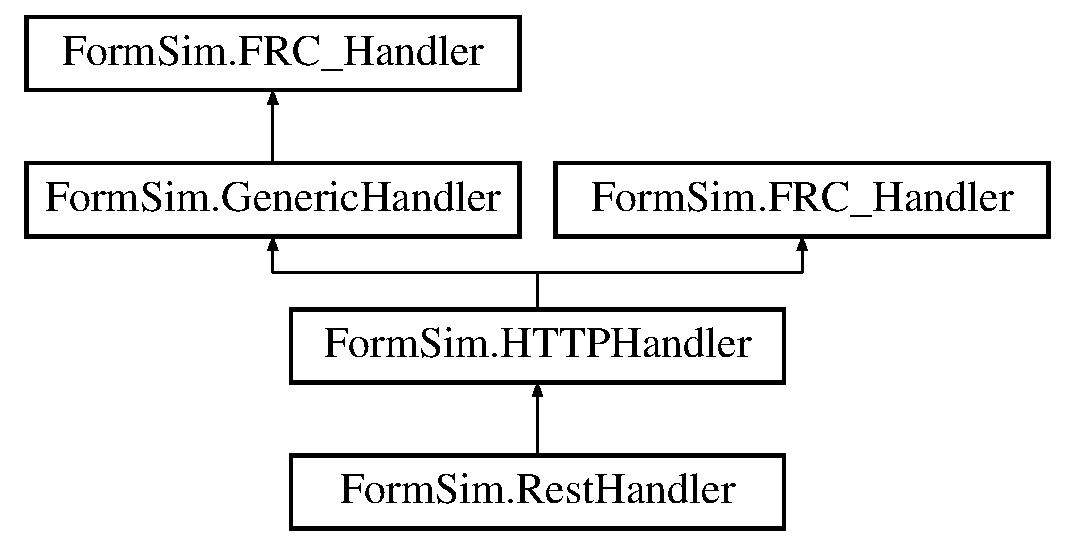
\includegraphics[height=4.000000cm]{class_form_sim_1_1_h_t_t_p_handler}
\end{center}
\end{figure}
\subsection*{Public Member Functions}
\begin{DoxyCompactItemize}
\item 
\mbox{\hyperlink{class_form_sim_1_1_h_t_t_p_handler_a8986ccceb64ce8804f354744961fc31f}{H\+T\+T\+P\+Handler}} ()
\item 
\mbox{\hyperlink{class_form_sim_1_1_h_t_t_p_handler_a2c39bc0dae5d5f2b26a84b1867d6ca23}{H\+T\+T\+P\+Handler}} (string \mbox{\hyperlink{class_form_sim_1_1_generic_handler_a6699d8bfc9cd305baf30ab9413b21605}{Auth\+Token}}, string \mbox{\hyperlink{class_form_sim_1_1_generic_handler_ae1d2175b140f4c600d74bbab1e22714e}{Client\+G\+U\+ID}})
\item 
\mbox{\hyperlink{class_form_sim_1_1_h_t_t_p_handler_af7f2265f6f02187c1470ef72d1c68e95}{H\+T\+T\+P\+Handler}} (string \mbox{\hyperlink{class_form_sim_1_1_generic_handler_a6699d8bfc9cd305baf30ab9413b21605}{Auth\+Token}}, string \mbox{\hyperlink{class_form_sim_1_1_generic_handler_ae1d2175b140f4c600d74bbab1e22714e}{Client\+G\+U\+ID}}, string \mbox{\hyperlink{class_form_sim_1_1_generic_handler_a12b51dea082a4d40d86829802adf073b}{I\+P\+Address}}, string \mbox{\hyperlink{class_form_sim_1_1_generic_handler_ac6492bb3e4fbe8f66c97b00bd27020c1}{Port}})
\item 
override async Task$<$ bool $>$ \mbox{\hyperlink{class_form_sim_1_1_h_t_t_p_handler_ae2ace13d7dc63f0bf1e1ef1a41bf8a3e}{perform\+Token\+Exchange}} ()
\begin{DoxyCompactList}\small\item\em Performs the token exchange with the client\+G\+U\+ID and Auth Token in exchange for an access token. N\+O\+TE\+: Both the client\+G\+U\+ID and the Auth\+Token must have been previously set or token exchange will fail. See \mbox{\hyperlink{interface_form_sim_1_1_f_r_c___handler_a3c77b2e99c98553928e463a9cbb5f7d4}{set\+Client\+G\+U\+I\+D(string)}} A\+ND See \mbox{\hyperlink{interface_form_sim_1_1_f_r_c___handler_a1314ea0937067435e3326818baa9d0c1}{set\+Auth\+Token(string)}} \end{DoxyCompactList}\item 
override async Task$<$ Dictionary$<$ string, string $>$ $>$ \mbox{\hyperlink{class_form_sim_1_1_h_t_t_p_handler_a31006e646afd7cb331784dce27760d5b}{send\+Raw}} (string raw\+String)
\begin{DoxyCompactList}\small\item\em Sends a raw request to Shift4 for processing. This is mainly used as a debugging tool, to figure out if there are issues with the request, that can be deciphered ahead of hitting the Shift4 processing engine on the back side. This likely should be run in debug mode when full source is available as common errors that get thrown are not very descriptive. As time permits the error catching should be improved to hopefully throw more useful information about the actual error. \end{DoxyCompactList}\end{DoxyCompactItemize}
\subsection*{Protected Member Functions}
\begin{DoxyCompactItemize}
\item 
override async Task$<$ Dictionary$<$ string, string $>$ $>$ \mbox{\hyperlink{class_form_sim_1_1_h_t_t_p_handler_a1b87e232c94cf390f7a9656744006639}{perform\+Transaction}} (Dictionary$<$ string, string $>$ parameters)
\begin{DoxyCompactList}\small\item\em This method needs to be Overridden by a subclass. Method exists here only to allow complete compilation. \end{DoxyCompactList}\end{DoxyCompactItemize}
\subsection*{Protected Attributes}
\begin{DoxyCompactItemize}
\item 
Http\+Client \mbox{\hyperlink{class_form_sim_1_1_h_t_t_p_handler_a1ce7f8f2407501a53c791cc6323ea5c7}{client}}
\end{DoxyCompactItemize}
\subsection*{Private Member Functions}
\begin{DoxyCompactItemize}
\item 
Dictionary$<$ string, string $>$ \mbox{\hyperlink{class_form_sim_1_1_h_t_t_p_handler_a9b0d19f62c0e810686bfafe5b7c1635e}{void\+Transaction}} (Dictionary$<$ string, string $>$ req, Dictionary$<$ string, string $>$ res)
\item 
Dictionary$<$ string, string $>$ \mbox{\hyperlink{class_form_sim_1_1_h_t_t_p_handler_a2e859f7aba91e19ddd6fe09747798624}{build\+Request\+Dict}} (Dictionary$<$ string, string $>$ dict, Dictionary$<$ string, string $>$ parameters)
\item 
Dictionary$<$ string, string $>$ \mbox{\hyperlink{class_form_sim_1_1_h_t_t_p_handler_a0f7eb27aa7bec1bc6de7c09dc38e495b}{build\+Online\+Authorization}} (Dictionary$<$ string, string $>$ dict, Dictionary$<$ string, string $>$ parameters)
\item 
Dictionary$<$ string, string $>$ \mbox{\hyperlink{class_form_sim_1_1_h_t_t_p_handler_a4cef4b23aeadba8cf19be19c648558dc}{build\+Online\+Sale}} (Dictionary$<$ string, string $>$ dict, Dictionary$<$ string, string $>$ parameters)
\item 
Dictionary$<$ string, string $>$ \mbox{\hyperlink{class_form_sim_1_1_h_t_t_p_handler_a0e74ea17a4cc7936f0fed0bc7104aea1}{build\+Offline\+Authorization}} (Dictionary$<$ string, string $>$ dict, Dictionary$<$ string, string $>$ parameters)
\item 
Dictionary$<$ string, string $>$ \mbox{\hyperlink{class_form_sim_1_1_h_t_t_p_handler_a8655b924790704629c9c746baf03b8c7}{build\+Offline\+Sale}} (Dictionary$<$ string, string $>$ dict, Dictionary$<$ string, string $>$ parameters)
\item 
Dictionary$<$ string, string $>$ \mbox{\hyperlink{class_form_sim_1_1_h_t_t_p_handler_acf01dc8988fc697ac06f4f031f045451}{build\+Void}} (Dictionary$<$ string, string $>$ dict, Dictionary$<$ string, string $>$ parameters)
\item 
Dictionary$<$ string, string $>$ \mbox{\hyperlink{class_form_sim_1_1_h_t_t_p_handler_a4722e4a151dd9ad2a90bccf55957ade2}{build\+Get\+Invoice\+Information}} (Dictionary$<$ string, string $>$ dict, Dictionary$<$ string, string $>$ parameters)
\item 
Dictionary$<$ string, string $>$ \mbox{\hyperlink{class_form_sim_1_1_h_t_t_p_handler_af1bfad7b18ee1fda69eab925aad1adc1}{build\+Get\+D\+B\+A\+Information}} (Dictionary$<$ string, string $>$ dict, Dictionary$<$ string, string $>$ parameters)
\item 
Dictionary$<$ string, string $>$ \mbox{\hyperlink{class_form_sim_1_1_h_t_t_p_handler_a37b770bc060a902e4fe149731b04ce48}{build\+Upload\+Signature}} (Dictionary$<$ string, string $>$ dict, Dictionary$<$ string, string $>$ parameters)
\item 
Dictionary$<$ string, string $>$ \mbox{\hyperlink{class_form_sim_1_1_h_t_t_p_handler_af9078923d0db307f20ac054594cbcaee}{build\+Get\+Voice\+Center\+Information}} (Dictionary$<$ string, string $>$ dict, Dictionary$<$ string, string $>$ parameters)
\item 
Dictionary$<$ string, string $>$ \mbox{\hyperlink{class_form_sim_1_1_h_t_t_p_handler_a18341e43f3157b786d314d71f402767c}{build\+Identify\+Card\+Type}} (Dictionary$<$ string, string $>$ dict, Dictionary$<$ string, string $>$ parameters)
\item 
Dictionary$<$ string, string $>$ \mbox{\hyperlink{class_form_sim_1_1_h_t_t_p_handler_a3123725d76b87880efbaa48e83395e3d}{build\+Verify\+Card\+With\+Processor}} (Dictionary$<$ string, string $>$ dict, Dictionary$<$ string, string $>$ parameters)
\item 
Dictionary$<$ string, string $>$ \mbox{\hyperlink{class_form_sim_1_1_h_t_t_p_handler_aad07a15901dadcdaa347e2f7a374adeb}{build\+Prompt\+For\+Signature}} (Dictionary$<$ string, string $>$ dict, Dictionary$<$ string, string $>$ parameters)
\item 
Dictionary$<$ string, string $>$ \mbox{\hyperlink{class_form_sim_1_1_h_t_t_p_handler_a2530058a140656b8ca6648cf59dfb559}{build\+Get\+Four\+Words}} (Dictionary$<$ string, string $>$ dict, Dictionary$<$ string, string $>$ parameters)
\item 
Dictionary$<$ string, string $>$ \mbox{\hyperlink{class_form_sim_1_1_h_t_t_p_handler_a55e9535d4f93c663b081064b2935104e}{build\+Status\+Request}} (Dictionary$<$ string, string $>$ dict, Dictionary$<$ string, string $>$ parameters)
\item 
Dictionary$<$ string, string $>$ \mbox{\hyperlink{class_form_sim_1_1_h_t_t_p_handler_ab53093caf6299e315441805ae43eb57f}{build\+Print\+Receipt\+To\+P\+I\+N\+Pad}} (Dictionary$<$ string, string $>$ dict, Dictionary$<$ string, string $>$ parameters)
\item 
Dictionary$<$ string, string $>$ \mbox{\hyperlink{class_form_sim_1_1_h_t_t_p_handler_a867f024e3e119d6601814e41a63ce2d5}{build\+Get\+Device\+Information}} (Dictionary$<$ string, string $>$ dict, Dictionary$<$ string, string $>$ parameters)
\item 
Dictionary$<$ string, string $>$ \mbox{\hyperlink{class_form_sim_1_1_h_t_t_p_handler_a4789d729c73cbc504c637df203773492}{build\+Prompt\+For\+Confirmation}} (Dictionary$<$ string, string $>$ dict, Dictionary$<$ string, string $>$ parameters)
\item 
Dictionary$<$ string, string $>$ \mbox{\hyperlink{class_form_sim_1_1_h_t_t_p_handler_a4cba54d2579ac2e2d4092e4a82c86d78}{build\+Display\+Custom\+Form}} (Dictionary$<$ string, string $>$ dict, Dictionary$<$ string, string $>$ parameters)
\item 
Dictionary$<$ string, string $>$ \mbox{\hyperlink{class_form_sim_1_1_h_t_t_p_handler_a0ad2f72ce6831fbe465bdb719216b002}{build\+Prompt\+For\+Terms\+And\+Conditions}} (Dictionary$<$ string, string $>$ dict, Dictionary$<$ string, string $>$ parameters)
\item 
Dictionary$<$ string, string $>$ \mbox{\hyperlink{class_form_sim_1_1_h_t_t_p_handler_a13ec56dae880175a2819b233a784fa58}{build\+On\+Demand\+Card\+Read}} (Dictionary$<$ string, string $>$ dict, Dictionary$<$ string, string $>$ parameters)
\item 
Dictionary$<$ string, string $>$ \mbox{\hyperlink{class_form_sim_1_1_h_t_t_p_handler_ab744b8ed04ff82ee322455a18010088e}{build\+Prompt\+For\+Input}} (Dictionary$<$ string, string $>$ dict, Dictionary$<$ string, string $>$ parameters)
\item 
Dictionary$<$ string, string $>$ \mbox{\hyperlink{class_form_sim_1_1_h_t_t_p_handler_a8163fc14a37997892b3ef79dbd8bc102}{build\+Get\+Acceptable\+I\+D\+Types\+For\+Checks}} (Dictionary$<$ string, string $>$ dict, Dictionary$<$ string, string $>$ parameters)
\item 
Dictionary$<$ string, string $>$ \mbox{\hyperlink{class_form_sim_1_1_h_t_t_p_handler_a140dfbd9d5456ac5cf76ff62cb0038ab}{build\+Check\+Approval}} (Dictionary$<$ string, string $>$ dict, Dictionary$<$ string, string $>$ parameters)
\item 
Dictionary$<$ string, string $>$ \mbox{\hyperlink{class_form_sim_1_1_h_t_t_p_handler_a44257bb4e9b6bec6569b19c9cd2114ac}{build\+Get\+Totals\+Report}} (Dictionary$<$ string, string $>$ dict, Dictionary$<$ string, string $>$ parameters)
\item 
Dictionary$<$ string, string $>$ \mbox{\hyperlink{class_form_sim_1_1_h_t_t_p_handler_a2f2aac001bdf4dd8fe64303c65532c5d}{build\+Display\+Line\+Item}} (Dictionary$<$ string, string $>$ dict, Dictionary$<$ string, string $>$ parameters)
\item 
Dictionary$<$ string, string $>$ \mbox{\hyperlink{class_form_sim_1_1_h_t_t_p_handler_a79ebd2df24f5098987e523c9c0bd6da4}{build\+Clear\+Line\+Items}} (Dictionary$<$ string, string $>$ dict, Dictionary$<$ string, string $>$ parameters)
\item 
Dictionary$<$ string, string $>$ \mbox{\hyperlink{class_form_sim_1_1_h_t_t_p_handler_a438c57cc6d6cc7afb0f73ec9771eaac8}{build\+Display\+Line\+Items}} (Dictionary$<$ string, string $>$ dict, Dictionary$<$ string, string $>$ parameters)
\item 
Dictionary$<$ string, string $>$ \mbox{\hyperlink{class_form_sim_1_1_h_t_t_p_handler_a11cc24e3e5d55dd5cece376b8eeafe6f}{build\+Swipe\+Ahead}} (Dictionary$<$ string, string $>$ dict, Dictionary$<$ string, string $>$ parameters)
\item 
Dictionary$<$ string, string $>$ \mbox{\hyperlink{class_form_sim_1_1_h_t_t_p_handler_a765f05cd55ea7dfd8b11e208451a80de}{build\+Reset\+P\+I\+N\+Pad}} (Dictionary$<$ string, string $>$ dict, Dictionary$<$ string, string $>$ parameters)
\item 
Dictionary$<$ string, string $>$ \mbox{\hyperlink{class_form_sim_1_1_h_t_t_p_handler_a5e51df91935179f2c7acfed9d783b6b4}{build\+Activate\+Reload\+Gift\+Card}} (Dictionary$<$ string, string $>$ dict, Dictionary$<$ string, string $>$ parameters)
\item 
Dictionary$<$ string, string $>$ \mbox{\hyperlink{class_form_sim_1_1_h_t_t_p_handler_a4bd3c7feb6f91dc88e657a619e7c263c}{build\+Deactivate\+Gift\+Card}} (Dictionary$<$ string, string $>$ dict, Dictionary$<$ string, string $>$ parameters)
\item 
Dictionary$<$ string, string $>$ \mbox{\hyperlink{class_form_sim_1_1_h_t_t_p_handler_af8e694086f55bb57f2819568b8a26eeb}{build\+Reactivate\+Gift\+Card}} (Dictionary$<$ string, string $>$ dict, Dictionary$<$ string, string $>$ parameters)
\item 
Dictionary$<$ string, string $>$ \mbox{\hyperlink{class_form_sim_1_1_h_t_t_p_handler_a956022ccfedfffe794e255be14d1121d}{build\+Get\+Balance\+Inquiry}} (Dictionary$<$ string, string $>$ dict, Dictionary$<$ string, string $>$ parameters)
\item 
Dictionary$<$ string, string $>$ \mbox{\hyperlink{class_form_sim_1_1_h_t_t_p_handler_ad44ba5b38c29b1ddd7fd87e35efa9157}{build\+Token\+Store\+Add}} (Dictionary$<$ string, string $>$ dict, Dictionary$<$ string, string $>$ parameters)
\item 
Dictionary$<$ string, string $>$ \mbox{\hyperlink{class_form_sim_1_1_h_t_t_p_handler_a12cf0f67fa1adf79e80ba68de9f06ab2}{build\+Token\+Store\+Duplicate}} (Dictionary$<$ string, string $>$ dict, Dictionary$<$ string, string $>$ parameters)
\item 
Dictionary$<$ string, string $>$ \mbox{\hyperlink{class_form_sim_1_1_h_t_t_p_handler_aa4d588b33663ae43ed124608bb0b2492}{build\+Block\+Card}} (Dictionary$<$ string, string $>$ dict, Dictionary$<$ string, string $>$ parameters)
\item 
Dictionary$<$ string, string $>$ \mbox{\hyperlink{class_form_sim_1_1_h_t_t_p_handler_ab579245ba4df602a3f5eb56d1107d0a5}{build\+Unblock\+Card}} (Dictionary$<$ string, string $>$ dict, Dictionary$<$ string, string $>$ parameters)
\item 
Dictionary$<$ string, string $>$ \mbox{\hyperlink{class_form_sim_1_1_h_t_t_p_handler_a847479885ccc06cb0925264bab2cb42f}{build\+Card\+Block\+Status}} (Dictionary$<$ string, string $>$ dict, Dictionary$<$ string, string $>$ parameters)
\item 
Dictionary$<$ string, string $>$ \mbox{\hyperlink{class_form_sim_1_1_h_t_t_p_handler_a5786e5a99e06dc5780fcecb076e3e570}{build\+Get\+Meta\+Token}} (Dictionary$<$ string, string $>$ dict, Dictionary$<$ string, string $>$ parameters)
\item 
Dictionary$<$ string, string $>$ \mbox{\hyperlink{class_form_sim_1_1_h_t_t_p_handler_af87ed1f553edd56103a99eb9fca49ce5}{build\+Level2\+Card\+Data}} (Dictionary$<$ string, string $>$ dict, Dictionary$<$ string, string $>$ parameters)
\item 
Dictionary$<$ string, string $>$ \mbox{\hyperlink{class_form_sim_1_1_h_t_t_p_handler_a19a204d9d4e398e1d4b7f96fe3a54d8f}{build\+Purchasing\+Card\+Data}} (Dictionary$<$ string, string $>$ dict, Dictionary$<$ string, string $>$ parameters)
\item 
Dictionary$<$ string, string $>$ \mbox{\hyperlink{class_form_sim_1_1_h_t_t_p_handler_ae36d78f08bb69c27da7e0c5d73b60db7}{build\+A\+V\+S\+Data}} (Dictionary$<$ string, string $>$ dict, Dictionary$<$ string, string $>$ parameters)
\item 
Dictionary$<$ string, string $>$ \mbox{\hyperlink{class_form_sim_1_1_h_t_t_p_handler_a16362967f4b50ff4a0b9a686cc7efd1a}{build\+Tip\+Data}} (Dictionary$<$ string, string $>$ dict, Dictionary$<$ string, string $>$ parameters)
\item 
Dictionary$<$ string, string $>$ \mbox{\hyperlink{class_form_sim_1_1_h_t_t_p_handler_a0e271753990736b71c2194688e1f55f8}{build\+Hotel\+Auth}} (Dictionary$<$ string, string $>$ dict, Dictionary$<$ string, string $>$ parameters)
\item 
Dictionary$<$ string, string $>$ \mbox{\hyperlink{class_form_sim_1_1_h_t_t_p_handler_a892cab2e68d920253f7efb8a9857bee4}{build\+Hotel\+Sale}} (Dictionary$<$ string, string $>$ dict, Dictionary$<$ string, string $>$ parameters)
\item 
Dictionary$<$ string, string $>$ \mbox{\hyperlink{class_form_sim_1_1_h_t_t_p_handler_a709759915daafeaf76b70ed470f07b33}{build\+Meta\+Token}} (Dictionary$<$ string, string $>$ dict, Dictionary$<$ string, string $>$ parameters)
\item 
Dictionary$<$ string, string $>$ \mbox{\hyperlink{class_form_sim_1_1_h_t_t_p_handler_a35e2a776065bad5b70c911ff946e9906}{build\+Misc\+Data}} (Dictionary$<$ string, string $>$ dict, Dictionary$<$ string, string $>$ parameters)
\item 
Dictionary$<$ string, string $>$ \mbox{\hyperlink{class_form_sim_1_1_h_t_t_p_handler_a817c861fd8d29ad2099c7e6abf4f0e7e}{build\+Token\+Store\+Data}} (Dictionary$<$ string, string $>$ dict, Dictionary$<$ string, string $>$ parameters)
\item 
Dictionary$<$ string, string $>$ \mbox{\hyperlink{class_form_sim_1_1_h_t_t_p_handler_a67afdc50b82e1d2ae539927867dcaa11}{build\+A\+V\+S\+\_\+\+C\+V\+V2\+Prompt\+Data}} (Dictionary$<$ string, string $>$ dict, Dictionary$<$ string, string $>$ parameters)
\item 
Dictionary$<$ string, string $>$ \mbox{\hyperlink{class_form_sim_1_1_h_t_t_p_handler_a8c0df472052df15698ec2693b7a90a39}{build\+Signature\+Capture\+Data}} (Dictionary$<$ string, string $>$ dict, Dictionary$<$ string, string $>$ parameters)
\item 
Dictionary$<$ string, string $>$ \mbox{\hyperlink{class_form_sim_1_1_h_t_t_p_handler_ad3eb4e695d351ec996c2e971f549c53f}{build\+H\+S\+A\+\_\+\+F\+S\+A\+Data}} (Dictionary$<$ string, string $>$ dict, Dictionary$<$ string, string $>$ parameters)
\item 
Dictionary$<$ string, string $>$ \mbox{\hyperlink{class_form_sim_1_1_h_t_t_p_handler_adee8ab1993ce8938e3f9239642aa5000}{build\+Non\+U\+T\+G\+Pin\+Debit\+Data}} (Dictionary$<$ string, string $>$ dict, Dictionary$<$ string, string $>$ parameters)
\item 
Dictionary$<$ string, string $>$ \mbox{\hyperlink{class_form_sim_1_1_h_t_t_p_handler_a585c3d76360835629effac14849d21f0}{build\+Auto\+Rental\+Auth\+Data}} (Dictionary$<$ string, string $>$ dict, Dictionary$<$ string, string $>$ parameters)
\item 
Dictionary$<$ string, string $>$ \mbox{\hyperlink{class_form_sim_1_1_h_t_t_p_handler_ae9695192a6ebc0698451b6e8b33fff83}{build\+Auto\+Rental\+Sale\+Data}} (Dictionary$<$ string, string $>$ dict, Dictionary$<$ string, string $>$ parameters)
\item 
bool \mbox{\hyperlink{class_form_sim_1_1_h_t_t_p_handler_a5c2cdcefdf8049706f6ce5d37a95114c}{parse\+Access\+Token}} (string results)
\item 
Dictionary$<$ string, string $>$ \mbox{\hyperlink{class_form_sim_1_1_h_t_t_p_handler_a3f81eb9021cb3b75427b4e1a84ee1529}{parse\+X\+M\+Lbased\+Results}} (string xml)
\end{DoxyCompactItemize}


\subsection{Detailed Description}
The \mbox{\hyperlink{class_form_sim_1_1_h_t_t_p_handler}{H\+T\+T\+P\+Handler}} class is designed to handle F\+R\+Cs over the H\+T\+TP protocol. Since this protocol uses key value pairs, it is important that the passed arguments be formatted and parsed correctly. This implementation handles both of those scenarios. See \mbox{\hyperlink{class_form_sim_1_1_generic_handler}{Generic\+Handler}} for the best implementation strategy of dealing with F\+R\+Cs in general. 



\subsection{Constructor \& Destructor Documentation}
\mbox{\Hypertarget{class_form_sim_1_1_h_t_t_p_handler_a8986ccceb64ce8804f354744961fc31f}\label{class_form_sim_1_1_h_t_t_p_handler_a8986ccceb64ce8804f354744961fc31f}} 
\index{Form\+Sim\+::\+H\+T\+T\+P\+Handler@{Form\+Sim\+::\+H\+T\+T\+P\+Handler}!H\+T\+T\+P\+Handler@{H\+T\+T\+P\+Handler}}
\index{H\+T\+T\+P\+Handler@{H\+T\+T\+P\+Handler}!Form\+Sim\+::\+H\+T\+T\+P\+Handler@{Form\+Sim\+::\+H\+T\+T\+P\+Handler}}
\subsubsection{\texorpdfstring{H\+T\+T\+P\+Handler()}{HTTPHandler()}\hspace{0.1cm}{\footnotesize\ttfamily [1/3]}}
{\footnotesize\ttfamily Form\+Sim.\+H\+T\+T\+P\+Handler.\+H\+T\+T\+P\+Handler (\begin{DoxyParamCaption}{ }\end{DoxyParamCaption})\hspace{0.3cm}{\ttfamily [inline]}}

\mbox{\Hypertarget{class_form_sim_1_1_h_t_t_p_handler_a2c39bc0dae5d5f2b26a84b1867d6ca23}\label{class_form_sim_1_1_h_t_t_p_handler_a2c39bc0dae5d5f2b26a84b1867d6ca23}} 
\index{Form\+Sim\+::\+H\+T\+T\+P\+Handler@{Form\+Sim\+::\+H\+T\+T\+P\+Handler}!H\+T\+T\+P\+Handler@{H\+T\+T\+P\+Handler}}
\index{H\+T\+T\+P\+Handler@{H\+T\+T\+P\+Handler}!Form\+Sim\+::\+H\+T\+T\+P\+Handler@{Form\+Sim\+::\+H\+T\+T\+P\+Handler}}
\subsubsection{\texorpdfstring{H\+T\+T\+P\+Handler()}{HTTPHandler()}\hspace{0.1cm}{\footnotesize\ttfamily [2/3]}}
{\footnotesize\ttfamily Form\+Sim.\+H\+T\+T\+P\+Handler.\+H\+T\+T\+P\+Handler (\begin{DoxyParamCaption}\item[{string}]{Auth\+Token,  }\item[{string}]{Client\+G\+U\+ID }\end{DoxyParamCaption})\hspace{0.3cm}{\ttfamily [inline]}}

\mbox{\Hypertarget{class_form_sim_1_1_h_t_t_p_handler_af7f2265f6f02187c1470ef72d1c68e95}\label{class_form_sim_1_1_h_t_t_p_handler_af7f2265f6f02187c1470ef72d1c68e95}} 
\index{Form\+Sim\+::\+H\+T\+T\+P\+Handler@{Form\+Sim\+::\+H\+T\+T\+P\+Handler}!H\+T\+T\+P\+Handler@{H\+T\+T\+P\+Handler}}
\index{H\+T\+T\+P\+Handler@{H\+T\+T\+P\+Handler}!Form\+Sim\+::\+H\+T\+T\+P\+Handler@{Form\+Sim\+::\+H\+T\+T\+P\+Handler}}
\subsubsection{\texorpdfstring{H\+T\+T\+P\+Handler()}{HTTPHandler()}\hspace{0.1cm}{\footnotesize\ttfamily [3/3]}}
{\footnotesize\ttfamily Form\+Sim.\+H\+T\+T\+P\+Handler.\+H\+T\+T\+P\+Handler (\begin{DoxyParamCaption}\item[{string}]{Auth\+Token,  }\item[{string}]{Client\+G\+U\+ID,  }\item[{string}]{I\+P\+Address,  }\item[{string}]{Port }\end{DoxyParamCaption})\hspace{0.3cm}{\ttfamily [inline]}}



\subsection{Member Function Documentation}
\mbox{\Hypertarget{class_form_sim_1_1_h_t_t_p_handler_a5e51df91935179f2c7acfed9d783b6b4}\label{class_form_sim_1_1_h_t_t_p_handler_a5e51df91935179f2c7acfed9d783b6b4}} 
\index{Form\+Sim\+::\+H\+T\+T\+P\+Handler@{Form\+Sim\+::\+H\+T\+T\+P\+Handler}!build\+Activate\+Reload\+Gift\+Card@{build\+Activate\+Reload\+Gift\+Card}}
\index{build\+Activate\+Reload\+Gift\+Card@{build\+Activate\+Reload\+Gift\+Card}!Form\+Sim\+::\+H\+T\+T\+P\+Handler@{Form\+Sim\+::\+H\+T\+T\+P\+Handler}}
\subsubsection{\texorpdfstring{build\+Activate\+Reload\+Gift\+Card()}{buildActivateReloadGiftCard()}}
{\footnotesize\ttfamily Dictionary$<$string, string$>$ Form\+Sim.\+H\+T\+T\+P\+Handler.\+build\+Activate\+Reload\+Gift\+Card (\begin{DoxyParamCaption}\item[{Dictionary$<$ string, string $>$}]{dict,  }\item[{Dictionary$<$ string, string $>$}]{parameters }\end{DoxyParamCaption})\hspace{0.3cm}{\ttfamily [inline]}, {\ttfamily [private]}}

\mbox{\Hypertarget{class_form_sim_1_1_h_t_t_p_handler_a585c3d76360835629effac14849d21f0}\label{class_form_sim_1_1_h_t_t_p_handler_a585c3d76360835629effac14849d21f0}} 
\index{Form\+Sim\+::\+H\+T\+T\+P\+Handler@{Form\+Sim\+::\+H\+T\+T\+P\+Handler}!build\+Auto\+Rental\+Auth\+Data@{build\+Auto\+Rental\+Auth\+Data}}
\index{build\+Auto\+Rental\+Auth\+Data@{build\+Auto\+Rental\+Auth\+Data}!Form\+Sim\+::\+H\+T\+T\+P\+Handler@{Form\+Sim\+::\+H\+T\+T\+P\+Handler}}
\subsubsection{\texorpdfstring{build\+Auto\+Rental\+Auth\+Data()}{buildAutoRentalAuthData()}}
{\footnotesize\ttfamily Dictionary$<$string, string$>$ Form\+Sim.\+H\+T\+T\+P\+Handler.\+build\+Auto\+Rental\+Auth\+Data (\begin{DoxyParamCaption}\item[{Dictionary$<$ string, string $>$}]{dict,  }\item[{Dictionary$<$ string, string $>$}]{parameters }\end{DoxyParamCaption})\hspace{0.3cm}{\ttfamily [inline]}, {\ttfamily [private]}}

\mbox{\Hypertarget{class_form_sim_1_1_h_t_t_p_handler_ae9695192a6ebc0698451b6e8b33fff83}\label{class_form_sim_1_1_h_t_t_p_handler_ae9695192a6ebc0698451b6e8b33fff83}} 
\index{Form\+Sim\+::\+H\+T\+T\+P\+Handler@{Form\+Sim\+::\+H\+T\+T\+P\+Handler}!build\+Auto\+Rental\+Sale\+Data@{build\+Auto\+Rental\+Sale\+Data}}
\index{build\+Auto\+Rental\+Sale\+Data@{build\+Auto\+Rental\+Sale\+Data}!Form\+Sim\+::\+H\+T\+T\+P\+Handler@{Form\+Sim\+::\+H\+T\+T\+P\+Handler}}
\subsubsection{\texorpdfstring{build\+Auto\+Rental\+Sale\+Data()}{buildAutoRentalSaleData()}}
{\footnotesize\ttfamily Dictionary$<$string, string$>$ Form\+Sim.\+H\+T\+T\+P\+Handler.\+build\+Auto\+Rental\+Sale\+Data (\begin{DoxyParamCaption}\item[{Dictionary$<$ string, string $>$}]{dict,  }\item[{Dictionary$<$ string, string $>$}]{parameters }\end{DoxyParamCaption})\hspace{0.3cm}{\ttfamily [inline]}, {\ttfamily [private]}}

\mbox{\Hypertarget{class_form_sim_1_1_h_t_t_p_handler_a67afdc50b82e1d2ae539927867dcaa11}\label{class_form_sim_1_1_h_t_t_p_handler_a67afdc50b82e1d2ae539927867dcaa11}} 
\index{Form\+Sim\+::\+H\+T\+T\+P\+Handler@{Form\+Sim\+::\+H\+T\+T\+P\+Handler}!build\+A\+V\+S\+\_\+\+C\+V\+V2\+Prompt\+Data@{build\+A\+V\+S\+\_\+\+C\+V\+V2\+Prompt\+Data}}
\index{build\+A\+V\+S\+\_\+\+C\+V\+V2\+Prompt\+Data@{build\+A\+V\+S\+\_\+\+C\+V\+V2\+Prompt\+Data}!Form\+Sim\+::\+H\+T\+T\+P\+Handler@{Form\+Sim\+::\+H\+T\+T\+P\+Handler}}
\subsubsection{\texorpdfstring{build\+A\+V\+S\+\_\+\+C\+V\+V2\+Prompt\+Data()}{buildAVS\_CVV2PromptData()}}
{\footnotesize\ttfamily Dictionary$<$string, string$>$ Form\+Sim.\+H\+T\+T\+P\+Handler.\+build\+A\+V\+S\+\_\+\+C\+V\+V2\+Prompt\+Data (\begin{DoxyParamCaption}\item[{Dictionary$<$ string, string $>$}]{dict,  }\item[{Dictionary$<$ string, string $>$}]{parameters }\end{DoxyParamCaption})\hspace{0.3cm}{\ttfamily [inline]}, {\ttfamily [private]}}

\mbox{\Hypertarget{class_form_sim_1_1_h_t_t_p_handler_ae36d78f08bb69c27da7e0c5d73b60db7}\label{class_form_sim_1_1_h_t_t_p_handler_ae36d78f08bb69c27da7e0c5d73b60db7}} 
\index{Form\+Sim\+::\+H\+T\+T\+P\+Handler@{Form\+Sim\+::\+H\+T\+T\+P\+Handler}!build\+A\+V\+S\+Data@{build\+A\+V\+S\+Data}}
\index{build\+A\+V\+S\+Data@{build\+A\+V\+S\+Data}!Form\+Sim\+::\+H\+T\+T\+P\+Handler@{Form\+Sim\+::\+H\+T\+T\+P\+Handler}}
\subsubsection{\texorpdfstring{build\+A\+V\+S\+Data()}{buildAVSData()}}
{\footnotesize\ttfamily Dictionary$<$string, string$>$ Form\+Sim.\+H\+T\+T\+P\+Handler.\+build\+A\+V\+S\+Data (\begin{DoxyParamCaption}\item[{Dictionary$<$ string, string $>$}]{dict,  }\item[{Dictionary$<$ string, string $>$}]{parameters }\end{DoxyParamCaption})\hspace{0.3cm}{\ttfamily [inline]}, {\ttfamily [private]}}

\mbox{\Hypertarget{class_form_sim_1_1_h_t_t_p_handler_aa4d588b33663ae43ed124608bb0b2492}\label{class_form_sim_1_1_h_t_t_p_handler_aa4d588b33663ae43ed124608bb0b2492}} 
\index{Form\+Sim\+::\+H\+T\+T\+P\+Handler@{Form\+Sim\+::\+H\+T\+T\+P\+Handler}!build\+Block\+Card@{build\+Block\+Card}}
\index{build\+Block\+Card@{build\+Block\+Card}!Form\+Sim\+::\+H\+T\+T\+P\+Handler@{Form\+Sim\+::\+H\+T\+T\+P\+Handler}}
\subsubsection{\texorpdfstring{build\+Block\+Card()}{buildBlockCard()}}
{\footnotesize\ttfamily Dictionary$<$string, string$>$ Form\+Sim.\+H\+T\+T\+P\+Handler.\+build\+Block\+Card (\begin{DoxyParamCaption}\item[{Dictionary$<$ string, string $>$}]{dict,  }\item[{Dictionary$<$ string, string $>$}]{parameters }\end{DoxyParamCaption})\hspace{0.3cm}{\ttfamily [inline]}, {\ttfamily [private]}}

\mbox{\Hypertarget{class_form_sim_1_1_h_t_t_p_handler_a847479885ccc06cb0925264bab2cb42f}\label{class_form_sim_1_1_h_t_t_p_handler_a847479885ccc06cb0925264bab2cb42f}} 
\index{Form\+Sim\+::\+H\+T\+T\+P\+Handler@{Form\+Sim\+::\+H\+T\+T\+P\+Handler}!build\+Card\+Block\+Status@{build\+Card\+Block\+Status}}
\index{build\+Card\+Block\+Status@{build\+Card\+Block\+Status}!Form\+Sim\+::\+H\+T\+T\+P\+Handler@{Form\+Sim\+::\+H\+T\+T\+P\+Handler}}
\subsubsection{\texorpdfstring{build\+Card\+Block\+Status()}{buildCardBlockStatus()}}
{\footnotesize\ttfamily Dictionary$<$string, string$>$ Form\+Sim.\+H\+T\+T\+P\+Handler.\+build\+Card\+Block\+Status (\begin{DoxyParamCaption}\item[{Dictionary$<$ string, string $>$}]{dict,  }\item[{Dictionary$<$ string, string $>$}]{parameters }\end{DoxyParamCaption})\hspace{0.3cm}{\ttfamily [inline]}, {\ttfamily [private]}}

\mbox{\Hypertarget{class_form_sim_1_1_h_t_t_p_handler_a140dfbd9d5456ac5cf76ff62cb0038ab}\label{class_form_sim_1_1_h_t_t_p_handler_a140dfbd9d5456ac5cf76ff62cb0038ab}} 
\index{Form\+Sim\+::\+H\+T\+T\+P\+Handler@{Form\+Sim\+::\+H\+T\+T\+P\+Handler}!build\+Check\+Approval@{build\+Check\+Approval}}
\index{build\+Check\+Approval@{build\+Check\+Approval}!Form\+Sim\+::\+H\+T\+T\+P\+Handler@{Form\+Sim\+::\+H\+T\+T\+P\+Handler}}
\subsubsection{\texorpdfstring{build\+Check\+Approval()}{buildCheckApproval()}}
{\footnotesize\ttfamily Dictionary$<$string, string$>$ Form\+Sim.\+H\+T\+T\+P\+Handler.\+build\+Check\+Approval (\begin{DoxyParamCaption}\item[{Dictionary$<$ string, string $>$}]{dict,  }\item[{Dictionary$<$ string, string $>$}]{parameters }\end{DoxyParamCaption})\hspace{0.3cm}{\ttfamily [inline]}, {\ttfamily [private]}}

\mbox{\Hypertarget{class_form_sim_1_1_h_t_t_p_handler_a79ebd2df24f5098987e523c9c0bd6da4}\label{class_form_sim_1_1_h_t_t_p_handler_a79ebd2df24f5098987e523c9c0bd6da4}} 
\index{Form\+Sim\+::\+H\+T\+T\+P\+Handler@{Form\+Sim\+::\+H\+T\+T\+P\+Handler}!build\+Clear\+Line\+Items@{build\+Clear\+Line\+Items}}
\index{build\+Clear\+Line\+Items@{build\+Clear\+Line\+Items}!Form\+Sim\+::\+H\+T\+T\+P\+Handler@{Form\+Sim\+::\+H\+T\+T\+P\+Handler}}
\subsubsection{\texorpdfstring{build\+Clear\+Line\+Items()}{buildClearLineItems()}}
{\footnotesize\ttfamily Dictionary$<$string, string$>$ Form\+Sim.\+H\+T\+T\+P\+Handler.\+build\+Clear\+Line\+Items (\begin{DoxyParamCaption}\item[{Dictionary$<$ string, string $>$}]{dict,  }\item[{Dictionary$<$ string, string $>$}]{parameters }\end{DoxyParamCaption})\hspace{0.3cm}{\ttfamily [inline]}, {\ttfamily [private]}}

\mbox{\Hypertarget{class_form_sim_1_1_h_t_t_p_handler_a4bd3c7feb6f91dc88e657a619e7c263c}\label{class_form_sim_1_1_h_t_t_p_handler_a4bd3c7feb6f91dc88e657a619e7c263c}} 
\index{Form\+Sim\+::\+H\+T\+T\+P\+Handler@{Form\+Sim\+::\+H\+T\+T\+P\+Handler}!build\+Deactivate\+Gift\+Card@{build\+Deactivate\+Gift\+Card}}
\index{build\+Deactivate\+Gift\+Card@{build\+Deactivate\+Gift\+Card}!Form\+Sim\+::\+H\+T\+T\+P\+Handler@{Form\+Sim\+::\+H\+T\+T\+P\+Handler}}
\subsubsection{\texorpdfstring{build\+Deactivate\+Gift\+Card()}{buildDeactivateGiftCard()}}
{\footnotesize\ttfamily Dictionary$<$string, string$>$ Form\+Sim.\+H\+T\+T\+P\+Handler.\+build\+Deactivate\+Gift\+Card (\begin{DoxyParamCaption}\item[{Dictionary$<$ string, string $>$}]{dict,  }\item[{Dictionary$<$ string, string $>$}]{parameters }\end{DoxyParamCaption})\hspace{0.3cm}{\ttfamily [inline]}, {\ttfamily [private]}}

\mbox{\Hypertarget{class_form_sim_1_1_h_t_t_p_handler_a4cba54d2579ac2e2d4092e4a82c86d78}\label{class_form_sim_1_1_h_t_t_p_handler_a4cba54d2579ac2e2d4092e4a82c86d78}} 
\index{Form\+Sim\+::\+H\+T\+T\+P\+Handler@{Form\+Sim\+::\+H\+T\+T\+P\+Handler}!build\+Display\+Custom\+Form@{build\+Display\+Custom\+Form}}
\index{build\+Display\+Custom\+Form@{build\+Display\+Custom\+Form}!Form\+Sim\+::\+H\+T\+T\+P\+Handler@{Form\+Sim\+::\+H\+T\+T\+P\+Handler}}
\subsubsection{\texorpdfstring{build\+Display\+Custom\+Form()}{buildDisplayCustomForm()}}
{\footnotesize\ttfamily Dictionary$<$string, string$>$ Form\+Sim.\+H\+T\+T\+P\+Handler.\+build\+Display\+Custom\+Form (\begin{DoxyParamCaption}\item[{Dictionary$<$ string, string $>$}]{dict,  }\item[{Dictionary$<$ string, string $>$}]{parameters }\end{DoxyParamCaption})\hspace{0.3cm}{\ttfamily [inline]}, {\ttfamily [private]}}

\mbox{\Hypertarget{class_form_sim_1_1_h_t_t_p_handler_a2f2aac001bdf4dd8fe64303c65532c5d}\label{class_form_sim_1_1_h_t_t_p_handler_a2f2aac001bdf4dd8fe64303c65532c5d}} 
\index{Form\+Sim\+::\+H\+T\+T\+P\+Handler@{Form\+Sim\+::\+H\+T\+T\+P\+Handler}!build\+Display\+Line\+Item@{build\+Display\+Line\+Item}}
\index{build\+Display\+Line\+Item@{build\+Display\+Line\+Item}!Form\+Sim\+::\+H\+T\+T\+P\+Handler@{Form\+Sim\+::\+H\+T\+T\+P\+Handler}}
\subsubsection{\texorpdfstring{build\+Display\+Line\+Item()}{buildDisplayLineItem()}}
{\footnotesize\ttfamily Dictionary$<$string, string$>$ Form\+Sim.\+H\+T\+T\+P\+Handler.\+build\+Display\+Line\+Item (\begin{DoxyParamCaption}\item[{Dictionary$<$ string, string $>$}]{dict,  }\item[{Dictionary$<$ string, string $>$}]{parameters }\end{DoxyParamCaption})\hspace{0.3cm}{\ttfamily [inline]}, {\ttfamily [private]}}

\mbox{\Hypertarget{class_form_sim_1_1_h_t_t_p_handler_a438c57cc6d6cc7afb0f73ec9771eaac8}\label{class_form_sim_1_1_h_t_t_p_handler_a438c57cc6d6cc7afb0f73ec9771eaac8}} 
\index{Form\+Sim\+::\+H\+T\+T\+P\+Handler@{Form\+Sim\+::\+H\+T\+T\+P\+Handler}!build\+Display\+Line\+Items@{build\+Display\+Line\+Items}}
\index{build\+Display\+Line\+Items@{build\+Display\+Line\+Items}!Form\+Sim\+::\+H\+T\+T\+P\+Handler@{Form\+Sim\+::\+H\+T\+T\+P\+Handler}}
\subsubsection{\texorpdfstring{build\+Display\+Line\+Items()}{buildDisplayLineItems()}}
{\footnotesize\ttfamily Dictionary$<$string, string$>$ Form\+Sim.\+H\+T\+T\+P\+Handler.\+build\+Display\+Line\+Items (\begin{DoxyParamCaption}\item[{Dictionary$<$ string, string $>$}]{dict,  }\item[{Dictionary$<$ string, string $>$}]{parameters }\end{DoxyParamCaption})\hspace{0.3cm}{\ttfamily [inline]}, {\ttfamily [private]}}

\mbox{\Hypertarget{class_form_sim_1_1_h_t_t_p_handler_a8163fc14a37997892b3ef79dbd8bc102}\label{class_form_sim_1_1_h_t_t_p_handler_a8163fc14a37997892b3ef79dbd8bc102}} 
\index{Form\+Sim\+::\+H\+T\+T\+P\+Handler@{Form\+Sim\+::\+H\+T\+T\+P\+Handler}!build\+Get\+Acceptable\+I\+D\+Types\+For\+Checks@{build\+Get\+Acceptable\+I\+D\+Types\+For\+Checks}}
\index{build\+Get\+Acceptable\+I\+D\+Types\+For\+Checks@{build\+Get\+Acceptable\+I\+D\+Types\+For\+Checks}!Form\+Sim\+::\+H\+T\+T\+P\+Handler@{Form\+Sim\+::\+H\+T\+T\+P\+Handler}}
\subsubsection{\texorpdfstring{build\+Get\+Acceptable\+I\+D\+Types\+For\+Checks()}{buildGetAcceptableIDTypesForChecks()}}
{\footnotesize\ttfamily Dictionary$<$string, string$>$ Form\+Sim.\+H\+T\+T\+P\+Handler.\+build\+Get\+Acceptable\+I\+D\+Types\+For\+Checks (\begin{DoxyParamCaption}\item[{Dictionary$<$ string, string $>$}]{dict,  }\item[{Dictionary$<$ string, string $>$}]{parameters }\end{DoxyParamCaption})\hspace{0.3cm}{\ttfamily [inline]}, {\ttfamily [private]}}

\mbox{\Hypertarget{class_form_sim_1_1_h_t_t_p_handler_a956022ccfedfffe794e255be14d1121d}\label{class_form_sim_1_1_h_t_t_p_handler_a956022ccfedfffe794e255be14d1121d}} 
\index{Form\+Sim\+::\+H\+T\+T\+P\+Handler@{Form\+Sim\+::\+H\+T\+T\+P\+Handler}!build\+Get\+Balance\+Inquiry@{build\+Get\+Balance\+Inquiry}}
\index{build\+Get\+Balance\+Inquiry@{build\+Get\+Balance\+Inquiry}!Form\+Sim\+::\+H\+T\+T\+P\+Handler@{Form\+Sim\+::\+H\+T\+T\+P\+Handler}}
\subsubsection{\texorpdfstring{build\+Get\+Balance\+Inquiry()}{buildGetBalanceInquiry()}}
{\footnotesize\ttfamily Dictionary$<$string, string$>$ Form\+Sim.\+H\+T\+T\+P\+Handler.\+build\+Get\+Balance\+Inquiry (\begin{DoxyParamCaption}\item[{Dictionary$<$ string, string $>$}]{dict,  }\item[{Dictionary$<$ string, string $>$}]{parameters }\end{DoxyParamCaption})\hspace{0.3cm}{\ttfamily [inline]}, {\ttfamily [private]}}

\mbox{\Hypertarget{class_form_sim_1_1_h_t_t_p_handler_af1bfad7b18ee1fda69eab925aad1adc1}\label{class_form_sim_1_1_h_t_t_p_handler_af1bfad7b18ee1fda69eab925aad1adc1}} 
\index{Form\+Sim\+::\+H\+T\+T\+P\+Handler@{Form\+Sim\+::\+H\+T\+T\+P\+Handler}!build\+Get\+D\+B\+A\+Information@{build\+Get\+D\+B\+A\+Information}}
\index{build\+Get\+D\+B\+A\+Information@{build\+Get\+D\+B\+A\+Information}!Form\+Sim\+::\+H\+T\+T\+P\+Handler@{Form\+Sim\+::\+H\+T\+T\+P\+Handler}}
\subsubsection{\texorpdfstring{build\+Get\+D\+B\+A\+Information()}{buildGetDBAInformation()}}
{\footnotesize\ttfamily Dictionary$<$string, string$>$ Form\+Sim.\+H\+T\+T\+P\+Handler.\+build\+Get\+D\+B\+A\+Information (\begin{DoxyParamCaption}\item[{Dictionary$<$ string, string $>$}]{dict,  }\item[{Dictionary$<$ string, string $>$}]{parameters }\end{DoxyParamCaption})\hspace{0.3cm}{\ttfamily [inline]}, {\ttfamily [private]}}

\mbox{\Hypertarget{class_form_sim_1_1_h_t_t_p_handler_a867f024e3e119d6601814e41a63ce2d5}\label{class_form_sim_1_1_h_t_t_p_handler_a867f024e3e119d6601814e41a63ce2d5}} 
\index{Form\+Sim\+::\+H\+T\+T\+P\+Handler@{Form\+Sim\+::\+H\+T\+T\+P\+Handler}!build\+Get\+Device\+Information@{build\+Get\+Device\+Information}}
\index{build\+Get\+Device\+Information@{build\+Get\+Device\+Information}!Form\+Sim\+::\+H\+T\+T\+P\+Handler@{Form\+Sim\+::\+H\+T\+T\+P\+Handler}}
\subsubsection{\texorpdfstring{build\+Get\+Device\+Information()}{buildGetDeviceInformation()}}
{\footnotesize\ttfamily Dictionary$<$string, string$>$ Form\+Sim.\+H\+T\+T\+P\+Handler.\+build\+Get\+Device\+Information (\begin{DoxyParamCaption}\item[{Dictionary$<$ string, string $>$}]{dict,  }\item[{Dictionary$<$ string, string $>$}]{parameters }\end{DoxyParamCaption})\hspace{0.3cm}{\ttfamily [inline]}, {\ttfamily [private]}}

\mbox{\Hypertarget{class_form_sim_1_1_h_t_t_p_handler_a2530058a140656b8ca6648cf59dfb559}\label{class_form_sim_1_1_h_t_t_p_handler_a2530058a140656b8ca6648cf59dfb559}} 
\index{Form\+Sim\+::\+H\+T\+T\+P\+Handler@{Form\+Sim\+::\+H\+T\+T\+P\+Handler}!build\+Get\+Four\+Words@{build\+Get\+Four\+Words}}
\index{build\+Get\+Four\+Words@{build\+Get\+Four\+Words}!Form\+Sim\+::\+H\+T\+T\+P\+Handler@{Form\+Sim\+::\+H\+T\+T\+P\+Handler}}
\subsubsection{\texorpdfstring{build\+Get\+Four\+Words()}{buildGetFourWords()}}
{\footnotesize\ttfamily Dictionary$<$string, string$>$ Form\+Sim.\+H\+T\+T\+P\+Handler.\+build\+Get\+Four\+Words (\begin{DoxyParamCaption}\item[{Dictionary$<$ string, string $>$}]{dict,  }\item[{Dictionary$<$ string, string $>$}]{parameters }\end{DoxyParamCaption})\hspace{0.3cm}{\ttfamily [inline]}, {\ttfamily [private]}}

\mbox{\Hypertarget{class_form_sim_1_1_h_t_t_p_handler_a4722e4a151dd9ad2a90bccf55957ade2}\label{class_form_sim_1_1_h_t_t_p_handler_a4722e4a151dd9ad2a90bccf55957ade2}} 
\index{Form\+Sim\+::\+H\+T\+T\+P\+Handler@{Form\+Sim\+::\+H\+T\+T\+P\+Handler}!build\+Get\+Invoice\+Information@{build\+Get\+Invoice\+Information}}
\index{build\+Get\+Invoice\+Information@{build\+Get\+Invoice\+Information}!Form\+Sim\+::\+H\+T\+T\+P\+Handler@{Form\+Sim\+::\+H\+T\+T\+P\+Handler}}
\subsubsection{\texorpdfstring{build\+Get\+Invoice\+Information()}{buildGetInvoiceInformation()}}
{\footnotesize\ttfamily Dictionary$<$string, string$>$ Form\+Sim.\+H\+T\+T\+P\+Handler.\+build\+Get\+Invoice\+Information (\begin{DoxyParamCaption}\item[{Dictionary$<$ string, string $>$}]{dict,  }\item[{Dictionary$<$ string, string $>$}]{parameters }\end{DoxyParamCaption})\hspace{0.3cm}{\ttfamily [inline]}, {\ttfamily [private]}}

\mbox{\Hypertarget{class_form_sim_1_1_h_t_t_p_handler_a5786e5a99e06dc5780fcecb076e3e570}\label{class_form_sim_1_1_h_t_t_p_handler_a5786e5a99e06dc5780fcecb076e3e570}} 
\index{Form\+Sim\+::\+H\+T\+T\+P\+Handler@{Form\+Sim\+::\+H\+T\+T\+P\+Handler}!build\+Get\+Meta\+Token@{build\+Get\+Meta\+Token}}
\index{build\+Get\+Meta\+Token@{build\+Get\+Meta\+Token}!Form\+Sim\+::\+H\+T\+T\+P\+Handler@{Form\+Sim\+::\+H\+T\+T\+P\+Handler}}
\subsubsection{\texorpdfstring{build\+Get\+Meta\+Token()}{buildGetMetaToken()}}
{\footnotesize\ttfamily Dictionary$<$string, string$>$ Form\+Sim.\+H\+T\+T\+P\+Handler.\+build\+Get\+Meta\+Token (\begin{DoxyParamCaption}\item[{Dictionary$<$ string, string $>$}]{dict,  }\item[{Dictionary$<$ string, string $>$}]{parameters }\end{DoxyParamCaption})\hspace{0.3cm}{\ttfamily [inline]}, {\ttfamily [private]}}

\mbox{\Hypertarget{class_form_sim_1_1_h_t_t_p_handler_a44257bb4e9b6bec6569b19c9cd2114ac}\label{class_form_sim_1_1_h_t_t_p_handler_a44257bb4e9b6bec6569b19c9cd2114ac}} 
\index{Form\+Sim\+::\+H\+T\+T\+P\+Handler@{Form\+Sim\+::\+H\+T\+T\+P\+Handler}!build\+Get\+Totals\+Report@{build\+Get\+Totals\+Report}}
\index{build\+Get\+Totals\+Report@{build\+Get\+Totals\+Report}!Form\+Sim\+::\+H\+T\+T\+P\+Handler@{Form\+Sim\+::\+H\+T\+T\+P\+Handler}}
\subsubsection{\texorpdfstring{build\+Get\+Totals\+Report()}{buildGetTotalsReport()}}
{\footnotesize\ttfamily Dictionary$<$string, string$>$ Form\+Sim.\+H\+T\+T\+P\+Handler.\+build\+Get\+Totals\+Report (\begin{DoxyParamCaption}\item[{Dictionary$<$ string, string $>$}]{dict,  }\item[{Dictionary$<$ string, string $>$}]{parameters }\end{DoxyParamCaption})\hspace{0.3cm}{\ttfamily [inline]}, {\ttfamily [private]}}

\mbox{\Hypertarget{class_form_sim_1_1_h_t_t_p_handler_af9078923d0db307f20ac054594cbcaee}\label{class_form_sim_1_1_h_t_t_p_handler_af9078923d0db307f20ac054594cbcaee}} 
\index{Form\+Sim\+::\+H\+T\+T\+P\+Handler@{Form\+Sim\+::\+H\+T\+T\+P\+Handler}!build\+Get\+Voice\+Center\+Information@{build\+Get\+Voice\+Center\+Information}}
\index{build\+Get\+Voice\+Center\+Information@{build\+Get\+Voice\+Center\+Information}!Form\+Sim\+::\+H\+T\+T\+P\+Handler@{Form\+Sim\+::\+H\+T\+T\+P\+Handler}}
\subsubsection{\texorpdfstring{build\+Get\+Voice\+Center\+Information()}{buildGetVoiceCenterInformation()}}
{\footnotesize\ttfamily Dictionary$<$string, string$>$ Form\+Sim.\+H\+T\+T\+P\+Handler.\+build\+Get\+Voice\+Center\+Information (\begin{DoxyParamCaption}\item[{Dictionary$<$ string, string $>$}]{dict,  }\item[{Dictionary$<$ string, string $>$}]{parameters }\end{DoxyParamCaption})\hspace{0.3cm}{\ttfamily [inline]}, {\ttfamily [private]}}

\mbox{\Hypertarget{class_form_sim_1_1_h_t_t_p_handler_a0e271753990736b71c2194688e1f55f8}\label{class_form_sim_1_1_h_t_t_p_handler_a0e271753990736b71c2194688e1f55f8}} 
\index{Form\+Sim\+::\+H\+T\+T\+P\+Handler@{Form\+Sim\+::\+H\+T\+T\+P\+Handler}!build\+Hotel\+Auth@{build\+Hotel\+Auth}}
\index{build\+Hotel\+Auth@{build\+Hotel\+Auth}!Form\+Sim\+::\+H\+T\+T\+P\+Handler@{Form\+Sim\+::\+H\+T\+T\+P\+Handler}}
\subsubsection{\texorpdfstring{build\+Hotel\+Auth()}{buildHotelAuth()}}
{\footnotesize\ttfamily Dictionary$<$string, string$>$ Form\+Sim.\+H\+T\+T\+P\+Handler.\+build\+Hotel\+Auth (\begin{DoxyParamCaption}\item[{Dictionary$<$ string, string $>$}]{dict,  }\item[{Dictionary$<$ string, string $>$}]{parameters }\end{DoxyParamCaption})\hspace{0.3cm}{\ttfamily [inline]}, {\ttfamily [private]}}

\mbox{\Hypertarget{class_form_sim_1_1_h_t_t_p_handler_a892cab2e68d920253f7efb8a9857bee4}\label{class_form_sim_1_1_h_t_t_p_handler_a892cab2e68d920253f7efb8a9857bee4}} 
\index{Form\+Sim\+::\+H\+T\+T\+P\+Handler@{Form\+Sim\+::\+H\+T\+T\+P\+Handler}!build\+Hotel\+Sale@{build\+Hotel\+Sale}}
\index{build\+Hotel\+Sale@{build\+Hotel\+Sale}!Form\+Sim\+::\+H\+T\+T\+P\+Handler@{Form\+Sim\+::\+H\+T\+T\+P\+Handler}}
\subsubsection{\texorpdfstring{build\+Hotel\+Sale()}{buildHotelSale()}}
{\footnotesize\ttfamily Dictionary$<$string, string$>$ Form\+Sim.\+H\+T\+T\+P\+Handler.\+build\+Hotel\+Sale (\begin{DoxyParamCaption}\item[{Dictionary$<$ string, string $>$}]{dict,  }\item[{Dictionary$<$ string, string $>$}]{parameters }\end{DoxyParamCaption})\hspace{0.3cm}{\ttfamily [inline]}, {\ttfamily [private]}}

\mbox{\Hypertarget{class_form_sim_1_1_h_t_t_p_handler_ad3eb4e695d351ec996c2e971f549c53f}\label{class_form_sim_1_1_h_t_t_p_handler_ad3eb4e695d351ec996c2e971f549c53f}} 
\index{Form\+Sim\+::\+H\+T\+T\+P\+Handler@{Form\+Sim\+::\+H\+T\+T\+P\+Handler}!build\+H\+S\+A\+\_\+\+F\+S\+A\+Data@{build\+H\+S\+A\+\_\+\+F\+S\+A\+Data}}
\index{build\+H\+S\+A\+\_\+\+F\+S\+A\+Data@{build\+H\+S\+A\+\_\+\+F\+S\+A\+Data}!Form\+Sim\+::\+H\+T\+T\+P\+Handler@{Form\+Sim\+::\+H\+T\+T\+P\+Handler}}
\subsubsection{\texorpdfstring{build\+H\+S\+A\+\_\+\+F\+S\+A\+Data()}{buildHSA\_FSAData()}}
{\footnotesize\ttfamily Dictionary$<$string, string$>$ Form\+Sim.\+H\+T\+T\+P\+Handler.\+build\+H\+S\+A\+\_\+\+F\+S\+A\+Data (\begin{DoxyParamCaption}\item[{Dictionary$<$ string, string $>$}]{dict,  }\item[{Dictionary$<$ string, string $>$}]{parameters }\end{DoxyParamCaption})\hspace{0.3cm}{\ttfamily [inline]}, {\ttfamily [private]}}

\mbox{\Hypertarget{class_form_sim_1_1_h_t_t_p_handler_a18341e43f3157b786d314d71f402767c}\label{class_form_sim_1_1_h_t_t_p_handler_a18341e43f3157b786d314d71f402767c}} 
\index{Form\+Sim\+::\+H\+T\+T\+P\+Handler@{Form\+Sim\+::\+H\+T\+T\+P\+Handler}!build\+Identify\+Card\+Type@{build\+Identify\+Card\+Type}}
\index{build\+Identify\+Card\+Type@{build\+Identify\+Card\+Type}!Form\+Sim\+::\+H\+T\+T\+P\+Handler@{Form\+Sim\+::\+H\+T\+T\+P\+Handler}}
\subsubsection{\texorpdfstring{build\+Identify\+Card\+Type()}{buildIdentifyCardType()}}
{\footnotesize\ttfamily Dictionary$<$string, string$>$ Form\+Sim.\+H\+T\+T\+P\+Handler.\+build\+Identify\+Card\+Type (\begin{DoxyParamCaption}\item[{Dictionary$<$ string, string $>$}]{dict,  }\item[{Dictionary$<$ string, string $>$}]{parameters }\end{DoxyParamCaption})\hspace{0.3cm}{\ttfamily [inline]}, {\ttfamily [private]}}

\mbox{\Hypertarget{class_form_sim_1_1_h_t_t_p_handler_af87ed1f553edd56103a99eb9fca49ce5}\label{class_form_sim_1_1_h_t_t_p_handler_af87ed1f553edd56103a99eb9fca49ce5}} 
\index{Form\+Sim\+::\+H\+T\+T\+P\+Handler@{Form\+Sim\+::\+H\+T\+T\+P\+Handler}!build\+Level2\+Card\+Data@{build\+Level2\+Card\+Data}}
\index{build\+Level2\+Card\+Data@{build\+Level2\+Card\+Data}!Form\+Sim\+::\+H\+T\+T\+P\+Handler@{Form\+Sim\+::\+H\+T\+T\+P\+Handler}}
\subsubsection{\texorpdfstring{build\+Level2\+Card\+Data()}{buildLevel2CardData()}}
{\footnotesize\ttfamily Dictionary$<$string, string$>$ Form\+Sim.\+H\+T\+T\+P\+Handler.\+build\+Level2\+Card\+Data (\begin{DoxyParamCaption}\item[{Dictionary$<$ string, string $>$}]{dict,  }\item[{Dictionary$<$ string, string $>$}]{parameters }\end{DoxyParamCaption})\hspace{0.3cm}{\ttfamily [inline]}, {\ttfamily [private]}}

\mbox{\Hypertarget{class_form_sim_1_1_h_t_t_p_handler_a709759915daafeaf76b70ed470f07b33}\label{class_form_sim_1_1_h_t_t_p_handler_a709759915daafeaf76b70ed470f07b33}} 
\index{Form\+Sim\+::\+H\+T\+T\+P\+Handler@{Form\+Sim\+::\+H\+T\+T\+P\+Handler}!build\+Meta\+Token@{build\+Meta\+Token}}
\index{build\+Meta\+Token@{build\+Meta\+Token}!Form\+Sim\+::\+H\+T\+T\+P\+Handler@{Form\+Sim\+::\+H\+T\+T\+P\+Handler}}
\subsubsection{\texorpdfstring{build\+Meta\+Token()}{buildMetaToken()}}
{\footnotesize\ttfamily Dictionary$<$string, string$>$ Form\+Sim.\+H\+T\+T\+P\+Handler.\+build\+Meta\+Token (\begin{DoxyParamCaption}\item[{Dictionary$<$ string, string $>$}]{dict,  }\item[{Dictionary$<$ string, string $>$}]{parameters }\end{DoxyParamCaption})\hspace{0.3cm}{\ttfamily [inline]}, {\ttfamily [private]}}

\mbox{\Hypertarget{class_form_sim_1_1_h_t_t_p_handler_a35e2a776065bad5b70c911ff946e9906}\label{class_form_sim_1_1_h_t_t_p_handler_a35e2a776065bad5b70c911ff946e9906}} 
\index{Form\+Sim\+::\+H\+T\+T\+P\+Handler@{Form\+Sim\+::\+H\+T\+T\+P\+Handler}!build\+Misc\+Data@{build\+Misc\+Data}}
\index{build\+Misc\+Data@{build\+Misc\+Data}!Form\+Sim\+::\+H\+T\+T\+P\+Handler@{Form\+Sim\+::\+H\+T\+T\+P\+Handler}}
\subsubsection{\texorpdfstring{build\+Misc\+Data()}{buildMiscData()}}
{\footnotesize\ttfamily Dictionary$<$string, string$>$ Form\+Sim.\+H\+T\+T\+P\+Handler.\+build\+Misc\+Data (\begin{DoxyParamCaption}\item[{Dictionary$<$ string, string $>$}]{dict,  }\item[{Dictionary$<$ string, string $>$}]{parameters }\end{DoxyParamCaption})\hspace{0.3cm}{\ttfamily [inline]}, {\ttfamily [private]}}

\mbox{\Hypertarget{class_form_sim_1_1_h_t_t_p_handler_adee8ab1993ce8938e3f9239642aa5000}\label{class_form_sim_1_1_h_t_t_p_handler_adee8ab1993ce8938e3f9239642aa5000}} 
\index{Form\+Sim\+::\+H\+T\+T\+P\+Handler@{Form\+Sim\+::\+H\+T\+T\+P\+Handler}!build\+Non\+U\+T\+G\+Pin\+Debit\+Data@{build\+Non\+U\+T\+G\+Pin\+Debit\+Data}}
\index{build\+Non\+U\+T\+G\+Pin\+Debit\+Data@{build\+Non\+U\+T\+G\+Pin\+Debit\+Data}!Form\+Sim\+::\+H\+T\+T\+P\+Handler@{Form\+Sim\+::\+H\+T\+T\+P\+Handler}}
\subsubsection{\texorpdfstring{build\+Non\+U\+T\+G\+Pin\+Debit\+Data()}{buildNonUTGPinDebitData()}}
{\footnotesize\ttfamily Dictionary$<$string, string$>$ Form\+Sim.\+H\+T\+T\+P\+Handler.\+build\+Non\+U\+T\+G\+Pin\+Debit\+Data (\begin{DoxyParamCaption}\item[{Dictionary$<$ string, string $>$}]{dict,  }\item[{Dictionary$<$ string, string $>$}]{parameters }\end{DoxyParamCaption})\hspace{0.3cm}{\ttfamily [inline]}, {\ttfamily [private]}}

\mbox{\Hypertarget{class_form_sim_1_1_h_t_t_p_handler_a0e74ea17a4cc7936f0fed0bc7104aea1}\label{class_form_sim_1_1_h_t_t_p_handler_a0e74ea17a4cc7936f0fed0bc7104aea1}} 
\index{Form\+Sim\+::\+H\+T\+T\+P\+Handler@{Form\+Sim\+::\+H\+T\+T\+P\+Handler}!build\+Offline\+Authorization@{build\+Offline\+Authorization}}
\index{build\+Offline\+Authorization@{build\+Offline\+Authorization}!Form\+Sim\+::\+H\+T\+T\+P\+Handler@{Form\+Sim\+::\+H\+T\+T\+P\+Handler}}
\subsubsection{\texorpdfstring{build\+Offline\+Authorization()}{buildOfflineAuthorization()}}
{\footnotesize\ttfamily Dictionary$<$string, string$>$ Form\+Sim.\+H\+T\+T\+P\+Handler.\+build\+Offline\+Authorization (\begin{DoxyParamCaption}\item[{Dictionary$<$ string, string $>$}]{dict,  }\item[{Dictionary$<$ string, string $>$}]{parameters }\end{DoxyParamCaption})\hspace{0.3cm}{\ttfamily [inline]}, {\ttfamily [private]}}

\mbox{\Hypertarget{class_form_sim_1_1_h_t_t_p_handler_a8655b924790704629c9c746baf03b8c7}\label{class_form_sim_1_1_h_t_t_p_handler_a8655b924790704629c9c746baf03b8c7}} 
\index{Form\+Sim\+::\+H\+T\+T\+P\+Handler@{Form\+Sim\+::\+H\+T\+T\+P\+Handler}!build\+Offline\+Sale@{build\+Offline\+Sale}}
\index{build\+Offline\+Sale@{build\+Offline\+Sale}!Form\+Sim\+::\+H\+T\+T\+P\+Handler@{Form\+Sim\+::\+H\+T\+T\+P\+Handler}}
\subsubsection{\texorpdfstring{build\+Offline\+Sale()}{buildOfflineSale()}}
{\footnotesize\ttfamily Dictionary$<$string, string$>$ Form\+Sim.\+H\+T\+T\+P\+Handler.\+build\+Offline\+Sale (\begin{DoxyParamCaption}\item[{Dictionary$<$ string, string $>$}]{dict,  }\item[{Dictionary$<$ string, string $>$}]{parameters }\end{DoxyParamCaption})\hspace{0.3cm}{\ttfamily [inline]}, {\ttfamily [private]}}

\mbox{\Hypertarget{class_form_sim_1_1_h_t_t_p_handler_a13ec56dae880175a2819b233a784fa58}\label{class_form_sim_1_1_h_t_t_p_handler_a13ec56dae880175a2819b233a784fa58}} 
\index{Form\+Sim\+::\+H\+T\+T\+P\+Handler@{Form\+Sim\+::\+H\+T\+T\+P\+Handler}!build\+On\+Demand\+Card\+Read@{build\+On\+Demand\+Card\+Read}}
\index{build\+On\+Demand\+Card\+Read@{build\+On\+Demand\+Card\+Read}!Form\+Sim\+::\+H\+T\+T\+P\+Handler@{Form\+Sim\+::\+H\+T\+T\+P\+Handler}}
\subsubsection{\texorpdfstring{build\+On\+Demand\+Card\+Read()}{buildOnDemandCardRead()}}
{\footnotesize\ttfamily Dictionary$<$string, string$>$ Form\+Sim.\+H\+T\+T\+P\+Handler.\+build\+On\+Demand\+Card\+Read (\begin{DoxyParamCaption}\item[{Dictionary$<$ string, string $>$}]{dict,  }\item[{Dictionary$<$ string, string $>$}]{parameters }\end{DoxyParamCaption})\hspace{0.3cm}{\ttfamily [inline]}, {\ttfamily [private]}}

\mbox{\Hypertarget{class_form_sim_1_1_h_t_t_p_handler_a0f7eb27aa7bec1bc6de7c09dc38e495b}\label{class_form_sim_1_1_h_t_t_p_handler_a0f7eb27aa7bec1bc6de7c09dc38e495b}} 
\index{Form\+Sim\+::\+H\+T\+T\+P\+Handler@{Form\+Sim\+::\+H\+T\+T\+P\+Handler}!build\+Online\+Authorization@{build\+Online\+Authorization}}
\index{build\+Online\+Authorization@{build\+Online\+Authorization}!Form\+Sim\+::\+H\+T\+T\+P\+Handler@{Form\+Sim\+::\+H\+T\+T\+P\+Handler}}
\subsubsection{\texorpdfstring{build\+Online\+Authorization()}{buildOnlineAuthorization()}}
{\footnotesize\ttfamily Dictionary$<$string, string$>$ Form\+Sim.\+H\+T\+T\+P\+Handler.\+build\+Online\+Authorization (\begin{DoxyParamCaption}\item[{Dictionary$<$ string, string $>$}]{dict,  }\item[{Dictionary$<$ string, string $>$}]{parameters }\end{DoxyParamCaption})\hspace{0.3cm}{\ttfamily [inline]}, {\ttfamily [private]}}

\mbox{\Hypertarget{class_form_sim_1_1_h_t_t_p_handler_a4cef4b23aeadba8cf19be19c648558dc}\label{class_form_sim_1_1_h_t_t_p_handler_a4cef4b23aeadba8cf19be19c648558dc}} 
\index{Form\+Sim\+::\+H\+T\+T\+P\+Handler@{Form\+Sim\+::\+H\+T\+T\+P\+Handler}!build\+Online\+Sale@{build\+Online\+Sale}}
\index{build\+Online\+Sale@{build\+Online\+Sale}!Form\+Sim\+::\+H\+T\+T\+P\+Handler@{Form\+Sim\+::\+H\+T\+T\+P\+Handler}}
\subsubsection{\texorpdfstring{build\+Online\+Sale()}{buildOnlineSale()}}
{\footnotesize\ttfamily Dictionary$<$string, string$>$ Form\+Sim.\+H\+T\+T\+P\+Handler.\+build\+Online\+Sale (\begin{DoxyParamCaption}\item[{Dictionary$<$ string, string $>$}]{dict,  }\item[{Dictionary$<$ string, string $>$}]{parameters }\end{DoxyParamCaption})\hspace{0.3cm}{\ttfamily [inline]}, {\ttfamily [private]}}

\mbox{\Hypertarget{class_form_sim_1_1_h_t_t_p_handler_ab53093caf6299e315441805ae43eb57f}\label{class_form_sim_1_1_h_t_t_p_handler_ab53093caf6299e315441805ae43eb57f}} 
\index{Form\+Sim\+::\+H\+T\+T\+P\+Handler@{Form\+Sim\+::\+H\+T\+T\+P\+Handler}!build\+Print\+Receipt\+To\+P\+I\+N\+Pad@{build\+Print\+Receipt\+To\+P\+I\+N\+Pad}}
\index{build\+Print\+Receipt\+To\+P\+I\+N\+Pad@{build\+Print\+Receipt\+To\+P\+I\+N\+Pad}!Form\+Sim\+::\+H\+T\+T\+P\+Handler@{Form\+Sim\+::\+H\+T\+T\+P\+Handler}}
\subsubsection{\texorpdfstring{build\+Print\+Receipt\+To\+P\+I\+N\+Pad()}{buildPrintReceiptToPINPad()}}
{\footnotesize\ttfamily Dictionary$<$string, string$>$ Form\+Sim.\+H\+T\+T\+P\+Handler.\+build\+Print\+Receipt\+To\+P\+I\+N\+Pad (\begin{DoxyParamCaption}\item[{Dictionary$<$ string, string $>$}]{dict,  }\item[{Dictionary$<$ string, string $>$}]{parameters }\end{DoxyParamCaption})\hspace{0.3cm}{\ttfamily [inline]}, {\ttfamily [private]}}

\mbox{\Hypertarget{class_form_sim_1_1_h_t_t_p_handler_a4789d729c73cbc504c637df203773492}\label{class_form_sim_1_1_h_t_t_p_handler_a4789d729c73cbc504c637df203773492}} 
\index{Form\+Sim\+::\+H\+T\+T\+P\+Handler@{Form\+Sim\+::\+H\+T\+T\+P\+Handler}!build\+Prompt\+For\+Confirmation@{build\+Prompt\+For\+Confirmation}}
\index{build\+Prompt\+For\+Confirmation@{build\+Prompt\+For\+Confirmation}!Form\+Sim\+::\+H\+T\+T\+P\+Handler@{Form\+Sim\+::\+H\+T\+T\+P\+Handler}}
\subsubsection{\texorpdfstring{build\+Prompt\+For\+Confirmation()}{buildPromptForConfirmation()}}
{\footnotesize\ttfamily Dictionary$<$string, string$>$ Form\+Sim.\+H\+T\+T\+P\+Handler.\+build\+Prompt\+For\+Confirmation (\begin{DoxyParamCaption}\item[{Dictionary$<$ string, string $>$}]{dict,  }\item[{Dictionary$<$ string, string $>$}]{parameters }\end{DoxyParamCaption})\hspace{0.3cm}{\ttfamily [inline]}, {\ttfamily [private]}}

\mbox{\Hypertarget{class_form_sim_1_1_h_t_t_p_handler_ab744b8ed04ff82ee322455a18010088e}\label{class_form_sim_1_1_h_t_t_p_handler_ab744b8ed04ff82ee322455a18010088e}} 
\index{Form\+Sim\+::\+H\+T\+T\+P\+Handler@{Form\+Sim\+::\+H\+T\+T\+P\+Handler}!build\+Prompt\+For\+Input@{build\+Prompt\+For\+Input}}
\index{build\+Prompt\+For\+Input@{build\+Prompt\+For\+Input}!Form\+Sim\+::\+H\+T\+T\+P\+Handler@{Form\+Sim\+::\+H\+T\+T\+P\+Handler}}
\subsubsection{\texorpdfstring{build\+Prompt\+For\+Input()}{buildPromptForInput()}}
{\footnotesize\ttfamily Dictionary$<$string, string$>$ Form\+Sim.\+H\+T\+T\+P\+Handler.\+build\+Prompt\+For\+Input (\begin{DoxyParamCaption}\item[{Dictionary$<$ string, string $>$}]{dict,  }\item[{Dictionary$<$ string, string $>$}]{parameters }\end{DoxyParamCaption})\hspace{0.3cm}{\ttfamily [inline]}, {\ttfamily [private]}}

\mbox{\Hypertarget{class_form_sim_1_1_h_t_t_p_handler_aad07a15901dadcdaa347e2f7a374adeb}\label{class_form_sim_1_1_h_t_t_p_handler_aad07a15901dadcdaa347e2f7a374adeb}} 
\index{Form\+Sim\+::\+H\+T\+T\+P\+Handler@{Form\+Sim\+::\+H\+T\+T\+P\+Handler}!build\+Prompt\+For\+Signature@{build\+Prompt\+For\+Signature}}
\index{build\+Prompt\+For\+Signature@{build\+Prompt\+For\+Signature}!Form\+Sim\+::\+H\+T\+T\+P\+Handler@{Form\+Sim\+::\+H\+T\+T\+P\+Handler}}
\subsubsection{\texorpdfstring{build\+Prompt\+For\+Signature()}{buildPromptForSignature()}}
{\footnotesize\ttfamily Dictionary$<$string, string$>$ Form\+Sim.\+H\+T\+T\+P\+Handler.\+build\+Prompt\+For\+Signature (\begin{DoxyParamCaption}\item[{Dictionary$<$ string, string $>$}]{dict,  }\item[{Dictionary$<$ string, string $>$}]{parameters }\end{DoxyParamCaption})\hspace{0.3cm}{\ttfamily [inline]}, {\ttfamily [private]}}

\mbox{\Hypertarget{class_form_sim_1_1_h_t_t_p_handler_a0ad2f72ce6831fbe465bdb719216b002}\label{class_form_sim_1_1_h_t_t_p_handler_a0ad2f72ce6831fbe465bdb719216b002}} 
\index{Form\+Sim\+::\+H\+T\+T\+P\+Handler@{Form\+Sim\+::\+H\+T\+T\+P\+Handler}!build\+Prompt\+For\+Terms\+And\+Conditions@{build\+Prompt\+For\+Terms\+And\+Conditions}}
\index{build\+Prompt\+For\+Terms\+And\+Conditions@{build\+Prompt\+For\+Terms\+And\+Conditions}!Form\+Sim\+::\+H\+T\+T\+P\+Handler@{Form\+Sim\+::\+H\+T\+T\+P\+Handler}}
\subsubsection{\texorpdfstring{build\+Prompt\+For\+Terms\+And\+Conditions()}{buildPromptForTermsAndConditions()}}
{\footnotesize\ttfamily Dictionary$<$string, string$>$ Form\+Sim.\+H\+T\+T\+P\+Handler.\+build\+Prompt\+For\+Terms\+And\+Conditions (\begin{DoxyParamCaption}\item[{Dictionary$<$ string, string $>$}]{dict,  }\item[{Dictionary$<$ string, string $>$}]{parameters }\end{DoxyParamCaption})\hspace{0.3cm}{\ttfamily [inline]}, {\ttfamily [private]}}

\mbox{\Hypertarget{class_form_sim_1_1_h_t_t_p_handler_a19a204d9d4e398e1d4b7f96fe3a54d8f}\label{class_form_sim_1_1_h_t_t_p_handler_a19a204d9d4e398e1d4b7f96fe3a54d8f}} 
\index{Form\+Sim\+::\+H\+T\+T\+P\+Handler@{Form\+Sim\+::\+H\+T\+T\+P\+Handler}!build\+Purchasing\+Card\+Data@{build\+Purchasing\+Card\+Data}}
\index{build\+Purchasing\+Card\+Data@{build\+Purchasing\+Card\+Data}!Form\+Sim\+::\+H\+T\+T\+P\+Handler@{Form\+Sim\+::\+H\+T\+T\+P\+Handler}}
\subsubsection{\texorpdfstring{build\+Purchasing\+Card\+Data()}{buildPurchasingCardData()}}
{\footnotesize\ttfamily Dictionary$<$string, string$>$ Form\+Sim.\+H\+T\+T\+P\+Handler.\+build\+Purchasing\+Card\+Data (\begin{DoxyParamCaption}\item[{Dictionary$<$ string, string $>$}]{dict,  }\item[{Dictionary$<$ string, string $>$}]{parameters }\end{DoxyParamCaption})\hspace{0.3cm}{\ttfamily [inline]}, {\ttfamily [private]}}

\mbox{\Hypertarget{class_form_sim_1_1_h_t_t_p_handler_af8e694086f55bb57f2819568b8a26eeb}\label{class_form_sim_1_1_h_t_t_p_handler_af8e694086f55bb57f2819568b8a26eeb}} 
\index{Form\+Sim\+::\+H\+T\+T\+P\+Handler@{Form\+Sim\+::\+H\+T\+T\+P\+Handler}!build\+Reactivate\+Gift\+Card@{build\+Reactivate\+Gift\+Card}}
\index{build\+Reactivate\+Gift\+Card@{build\+Reactivate\+Gift\+Card}!Form\+Sim\+::\+H\+T\+T\+P\+Handler@{Form\+Sim\+::\+H\+T\+T\+P\+Handler}}
\subsubsection{\texorpdfstring{build\+Reactivate\+Gift\+Card()}{buildReactivateGiftCard()}}
{\footnotesize\ttfamily Dictionary$<$string, string$>$ Form\+Sim.\+H\+T\+T\+P\+Handler.\+build\+Reactivate\+Gift\+Card (\begin{DoxyParamCaption}\item[{Dictionary$<$ string, string $>$}]{dict,  }\item[{Dictionary$<$ string, string $>$}]{parameters }\end{DoxyParamCaption})\hspace{0.3cm}{\ttfamily [inline]}, {\ttfamily [private]}}

\mbox{\Hypertarget{class_form_sim_1_1_h_t_t_p_handler_a2e859f7aba91e19ddd6fe09747798624}\label{class_form_sim_1_1_h_t_t_p_handler_a2e859f7aba91e19ddd6fe09747798624}} 
\index{Form\+Sim\+::\+H\+T\+T\+P\+Handler@{Form\+Sim\+::\+H\+T\+T\+P\+Handler}!build\+Request\+Dict@{build\+Request\+Dict}}
\index{build\+Request\+Dict@{build\+Request\+Dict}!Form\+Sim\+::\+H\+T\+T\+P\+Handler@{Form\+Sim\+::\+H\+T\+T\+P\+Handler}}
\subsubsection{\texorpdfstring{build\+Request\+Dict()}{buildRequestDict()}}
{\footnotesize\ttfamily Dictionary$<$string, string$>$ Form\+Sim.\+H\+T\+T\+P\+Handler.\+build\+Request\+Dict (\begin{DoxyParamCaption}\item[{Dictionary$<$ string, string $>$}]{dict,  }\item[{Dictionary$<$ string, string $>$}]{parameters }\end{DoxyParamCaption})\hspace{0.3cm}{\ttfamily [inline]}, {\ttfamily [private]}}

\mbox{\Hypertarget{class_form_sim_1_1_h_t_t_p_handler_a765f05cd55ea7dfd8b11e208451a80de}\label{class_form_sim_1_1_h_t_t_p_handler_a765f05cd55ea7dfd8b11e208451a80de}} 
\index{Form\+Sim\+::\+H\+T\+T\+P\+Handler@{Form\+Sim\+::\+H\+T\+T\+P\+Handler}!build\+Reset\+P\+I\+N\+Pad@{build\+Reset\+P\+I\+N\+Pad}}
\index{build\+Reset\+P\+I\+N\+Pad@{build\+Reset\+P\+I\+N\+Pad}!Form\+Sim\+::\+H\+T\+T\+P\+Handler@{Form\+Sim\+::\+H\+T\+T\+P\+Handler}}
\subsubsection{\texorpdfstring{build\+Reset\+P\+I\+N\+Pad()}{buildResetPINPad()}}
{\footnotesize\ttfamily Dictionary$<$string, string$>$ Form\+Sim.\+H\+T\+T\+P\+Handler.\+build\+Reset\+P\+I\+N\+Pad (\begin{DoxyParamCaption}\item[{Dictionary$<$ string, string $>$}]{dict,  }\item[{Dictionary$<$ string, string $>$}]{parameters }\end{DoxyParamCaption})\hspace{0.3cm}{\ttfamily [inline]}, {\ttfamily [private]}}

\mbox{\Hypertarget{class_form_sim_1_1_h_t_t_p_handler_a8c0df472052df15698ec2693b7a90a39}\label{class_form_sim_1_1_h_t_t_p_handler_a8c0df472052df15698ec2693b7a90a39}} 
\index{Form\+Sim\+::\+H\+T\+T\+P\+Handler@{Form\+Sim\+::\+H\+T\+T\+P\+Handler}!build\+Signature\+Capture\+Data@{build\+Signature\+Capture\+Data}}
\index{build\+Signature\+Capture\+Data@{build\+Signature\+Capture\+Data}!Form\+Sim\+::\+H\+T\+T\+P\+Handler@{Form\+Sim\+::\+H\+T\+T\+P\+Handler}}
\subsubsection{\texorpdfstring{build\+Signature\+Capture\+Data()}{buildSignatureCaptureData()}}
{\footnotesize\ttfamily Dictionary$<$string, string$>$ Form\+Sim.\+H\+T\+T\+P\+Handler.\+build\+Signature\+Capture\+Data (\begin{DoxyParamCaption}\item[{Dictionary$<$ string, string $>$}]{dict,  }\item[{Dictionary$<$ string, string $>$}]{parameters }\end{DoxyParamCaption})\hspace{0.3cm}{\ttfamily [inline]}, {\ttfamily [private]}}

\mbox{\Hypertarget{class_form_sim_1_1_h_t_t_p_handler_a55e9535d4f93c663b081064b2935104e}\label{class_form_sim_1_1_h_t_t_p_handler_a55e9535d4f93c663b081064b2935104e}} 
\index{Form\+Sim\+::\+H\+T\+T\+P\+Handler@{Form\+Sim\+::\+H\+T\+T\+P\+Handler}!build\+Status\+Request@{build\+Status\+Request}}
\index{build\+Status\+Request@{build\+Status\+Request}!Form\+Sim\+::\+H\+T\+T\+P\+Handler@{Form\+Sim\+::\+H\+T\+T\+P\+Handler}}
\subsubsection{\texorpdfstring{build\+Status\+Request()}{buildStatusRequest()}}
{\footnotesize\ttfamily Dictionary$<$string, string$>$ Form\+Sim.\+H\+T\+T\+P\+Handler.\+build\+Status\+Request (\begin{DoxyParamCaption}\item[{Dictionary$<$ string, string $>$}]{dict,  }\item[{Dictionary$<$ string, string $>$}]{parameters }\end{DoxyParamCaption})\hspace{0.3cm}{\ttfamily [inline]}, {\ttfamily [private]}}

\mbox{\Hypertarget{class_form_sim_1_1_h_t_t_p_handler_a11cc24e3e5d55dd5cece376b8eeafe6f}\label{class_form_sim_1_1_h_t_t_p_handler_a11cc24e3e5d55dd5cece376b8eeafe6f}} 
\index{Form\+Sim\+::\+H\+T\+T\+P\+Handler@{Form\+Sim\+::\+H\+T\+T\+P\+Handler}!build\+Swipe\+Ahead@{build\+Swipe\+Ahead}}
\index{build\+Swipe\+Ahead@{build\+Swipe\+Ahead}!Form\+Sim\+::\+H\+T\+T\+P\+Handler@{Form\+Sim\+::\+H\+T\+T\+P\+Handler}}
\subsubsection{\texorpdfstring{build\+Swipe\+Ahead()}{buildSwipeAhead()}}
{\footnotesize\ttfamily Dictionary$<$string, string$>$ Form\+Sim.\+H\+T\+T\+P\+Handler.\+build\+Swipe\+Ahead (\begin{DoxyParamCaption}\item[{Dictionary$<$ string, string $>$}]{dict,  }\item[{Dictionary$<$ string, string $>$}]{parameters }\end{DoxyParamCaption})\hspace{0.3cm}{\ttfamily [inline]}, {\ttfamily [private]}}

\mbox{\Hypertarget{class_form_sim_1_1_h_t_t_p_handler_a16362967f4b50ff4a0b9a686cc7efd1a}\label{class_form_sim_1_1_h_t_t_p_handler_a16362967f4b50ff4a0b9a686cc7efd1a}} 
\index{Form\+Sim\+::\+H\+T\+T\+P\+Handler@{Form\+Sim\+::\+H\+T\+T\+P\+Handler}!build\+Tip\+Data@{build\+Tip\+Data}}
\index{build\+Tip\+Data@{build\+Tip\+Data}!Form\+Sim\+::\+H\+T\+T\+P\+Handler@{Form\+Sim\+::\+H\+T\+T\+P\+Handler}}
\subsubsection{\texorpdfstring{build\+Tip\+Data()}{buildTipData()}}
{\footnotesize\ttfamily Dictionary$<$string, string$>$ Form\+Sim.\+H\+T\+T\+P\+Handler.\+build\+Tip\+Data (\begin{DoxyParamCaption}\item[{Dictionary$<$ string, string $>$}]{dict,  }\item[{Dictionary$<$ string, string $>$}]{parameters }\end{DoxyParamCaption})\hspace{0.3cm}{\ttfamily [inline]}, {\ttfamily [private]}}

\mbox{\Hypertarget{class_form_sim_1_1_h_t_t_p_handler_ad44ba5b38c29b1ddd7fd87e35efa9157}\label{class_form_sim_1_1_h_t_t_p_handler_ad44ba5b38c29b1ddd7fd87e35efa9157}} 
\index{Form\+Sim\+::\+H\+T\+T\+P\+Handler@{Form\+Sim\+::\+H\+T\+T\+P\+Handler}!build\+Token\+Store\+Add@{build\+Token\+Store\+Add}}
\index{build\+Token\+Store\+Add@{build\+Token\+Store\+Add}!Form\+Sim\+::\+H\+T\+T\+P\+Handler@{Form\+Sim\+::\+H\+T\+T\+P\+Handler}}
\subsubsection{\texorpdfstring{build\+Token\+Store\+Add()}{buildTokenStoreAdd()}}
{\footnotesize\ttfamily Dictionary$<$string, string$>$ Form\+Sim.\+H\+T\+T\+P\+Handler.\+build\+Token\+Store\+Add (\begin{DoxyParamCaption}\item[{Dictionary$<$ string, string $>$}]{dict,  }\item[{Dictionary$<$ string, string $>$}]{parameters }\end{DoxyParamCaption})\hspace{0.3cm}{\ttfamily [inline]}, {\ttfamily [private]}}

\mbox{\Hypertarget{class_form_sim_1_1_h_t_t_p_handler_a817c861fd8d29ad2099c7e6abf4f0e7e}\label{class_form_sim_1_1_h_t_t_p_handler_a817c861fd8d29ad2099c7e6abf4f0e7e}} 
\index{Form\+Sim\+::\+H\+T\+T\+P\+Handler@{Form\+Sim\+::\+H\+T\+T\+P\+Handler}!build\+Token\+Store\+Data@{build\+Token\+Store\+Data}}
\index{build\+Token\+Store\+Data@{build\+Token\+Store\+Data}!Form\+Sim\+::\+H\+T\+T\+P\+Handler@{Form\+Sim\+::\+H\+T\+T\+P\+Handler}}
\subsubsection{\texorpdfstring{build\+Token\+Store\+Data()}{buildTokenStoreData()}}
{\footnotesize\ttfamily Dictionary$<$string, string$>$ Form\+Sim.\+H\+T\+T\+P\+Handler.\+build\+Token\+Store\+Data (\begin{DoxyParamCaption}\item[{Dictionary$<$ string, string $>$}]{dict,  }\item[{Dictionary$<$ string, string $>$}]{parameters }\end{DoxyParamCaption})\hspace{0.3cm}{\ttfamily [inline]}, {\ttfamily [private]}}

\mbox{\Hypertarget{class_form_sim_1_1_h_t_t_p_handler_a12cf0f67fa1adf79e80ba68de9f06ab2}\label{class_form_sim_1_1_h_t_t_p_handler_a12cf0f67fa1adf79e80ba68de9f06ab2}} 
\index{Form\+Sim\+::\+H\+T\+T\+P\+Handler@{Form\+Sim\+::\+H\+T\+T\+P\+Handler}!build\+Token\+Store\+Duplicate@{build\+Token\+Store\+Duplicate}}
\index{build\+Token\+Store\+Duplicate@{build\+Token\+Store\+Duplicate}!Form\+Sim\+::\+H\+T\+T\+P\+Handler@{Form\+Sim\+::\+H\+T\+T\+P\+Handler}}
\subsubsection{\texorpdfstring{build\+Token\+Store\+Duplicate()}{buildTokenStoreDuplicate()}}
{\footnotesize\ttfamily Dictionary$<$string, string$>$ Form\+Sim.\+H\+T\+T\+P\+Handler.\+build\+Token\+Store\+Duplicate (\begin{DoxyParamCaption}\item[{Dictionary$<$ string, string $>$}]{dict,  }\item[{Dictionary$<$ string, string $>$}]{parameters }\end{DoxyParamCaption})\hspace{0.3cm}{\ttfamily [inline]}, {\ttfamily [private]}}

\mbox{\Hypertarget{class_form_sim_1_1_h_t_t_p_handler_ab579245ba4df602a3f5eb56d1107d0a5}\label{class_form_sim_1_1_h_t_t_p_handler_ab579245ba4df602a3f5eb56d1107d0a5}} 
\index{Form\+Sim\+::\+H\+T\+T\+P\+Handler@{Form\+Sim\+::\+H\+T\+T\+P\+Handler}!build\+Unblock\+Card@{build\+Unblock\+Card}}
\index{build\+Unblock\+Card@{build\+Unblock\+Card}!Form\+Sim\+::\+H\+T\+T\+P\+Handler@{Form\+Sim\+::\+H\+T\+T\+P\+Handler}}
\subsubsection{\texorpdfstring{build\+Unblock\+Card()}{buildUnblockCard()}}
{\footnotesize\ttfamily Dictionary$<$string, string$>$ Form\+Sim.\+H\+T\+T\+P\+Handler.\+build\+Unblock\+Card (\begin{DoxyParamCaption}\item[{Dictionary$<$ string, string $>$}]{dict,  }\item[{Dictionary$<$ string, string $>$}]{parameters }\end{DoxyParamCaption})\hspace{0.3cm}{\ttfamily [inline]}, {\ttfamily [private]}}

\mbox{\Hypertarget{class_form_sim_1_1_h_t_t_p_handler_a37b770bc060a902e4fe149731b04ce48}\label{class_form_sim_1_1_h_t_t_p_handler_a37b770bc060a902e4fe149731b04ce48}} 
\index{Form\+Sim\+::\+H\+T\+T\+P\+Handler@{Form\+Sim\+::\+H\+T\+T\+P\+Handler}!build\+Upload\+Signature@{build\+Upload\+Signature}}
\index{build\+Upload\+Signature@{build\+Upload\+Signature}!Form\+Sim\+::\+H\+T\+T\+P\+Handler@{Form\+Sim\+::\+H\+T\+T\+P\+Handler}}
\subsubsection{\texorpdfstring{build\+Upload\+Signature()}{buildUploadSignature()}}
{\footnotesize\ttfamily Dictionary$<$string, string$>$ Form\+Sim.\+H\+T\+T\+P\+Handler.\+build\+Upload\+Signature (\begin{DoxyParamCaption}\item[{Dictionary$<$ string, string $>$}]{dict,  }\item[{Dictionary$<$ string, string $>$}]{parameters }\end{DoxyParamCaption})\hspace{0.3cm}{\ttfamily [inline]}, {\ttfamily [private]}}

\mbox{\Hypertarget{class_form_sim_1_1_h_t_t_p_handler_a3123725d76b87880efbaa48e83395e3d}\label{class_form_sim_1_1_h_t_t_p_handler_a3123725d76b87880efbaa48e83395e3d}} 
\index{Form\+Sim\+::\+H\+T\+T\+P\+Handler@{Form\+Sim\+::\+H\+T\+T\+P\+Handler}!build\+Verify\+Card\+With\+Processor@{build\+Verify\+Card\+With\+Processor}}
\index{build\+Verify\+Card\+With\+Processor@{build\+Verify\+Card\+With\+Processor}!Form\+Sim\+::\+H\+T\+T\+P\+Handler@{Form\+Sim\+::\+H\+T\+T\+P\+Handler}}
\subsubsection{\texorpdfstring{build\+Verify\+Card\+With\+Processor()}{buildVerifyCardWithProcessor()}}
{\footnotesize\ttfamily Dictionary$<$string, string$>$ Form\+Sim.\+H\+T\+T\+P\+Handler.\+build\+Verify\+Card\+With\+Processor (\begin{DoxyParamCaption}\item[{Dictionary$<$ string, string $>$}]{dict,  }\item[{Dictionary$<$ string, string $>$}]{parameters }\end{DoxyParamCaption})\hspace{0.3cm}{\ttfamily [inline]}, {\ttfamily [private]}}

\mbox{\Hypertarget{class_form_sim_1_1_h_t_t_p_handler_acf01dc8988fc697ac06f4f031f045451}\label{class_form_sim_1_1_h_t_t_p_handler_acf01dc8988fc697ac06f4f031f045451}} 
\index{Form\+Sim\+::\+H\+T\+T\+P\+Handler@{Form\+Sim\+::\+H\+T\+T\+P\+Handler}!build\+Void@{build\+Void}}
\index{build\+Void@{build\+Void}!Form\+Sim\+::\+H\+T\+T\+P\+Handler@{Form\+Sim\+::\+H\+T\+T\+P\+Handler}}
\subsubsection{\texorpdfstring{build\+Void()}{buildVoid()}}
{\footnotesize\ttfamily Dictionary$<$string, string$>$ Form\+Sim.\+H\+T\+T\+P\+Handler.\+build\+Void (\begin{DoxyParamCaption}\item[{Dictionary$<$ string, string $>$}]{dict,  }\item[{Dictionary$<$ string, string $>$}]{parameters }\end{DoxyParamCaption})\hspace{0.3cm}{\ttfamily [inline]}, {\ttfamily [private]}}

\mbox{\Hypertarget{class_form_sim_1_1_h_t_t_p_handler_a5c2cdcefdf8049706f6ce5d37a95114c}\label{class_form_sim_1_1_h_t_t_p_handler_a5c2cdcefdf8049706f6ce5d37a95114c}} 
\index{Form\+Sim\+::\+H\+T\+T\+P\+Handler@{Form\+Sim\+::\+H\+T\+T\+P\+Handler}!parse\+Access\+Token@{parse\+Access\+Token}}
\index{parse\+Access\+Token@{parse\+Access\+Token}!Form\+Sim\+::\+H\+T\+T\+P\+Handler@{Form\+Sim\+::\+H\+T\+T\+P\+Handler}}
\subsubsection{\texorpdfstring{parse\+Access\+Token()}{parseAccessToken()}}
{\footnotesize\ttfamily bool Form\+Sim.\+H\+T\+T\+P\+Handler.\+parse\+Access\+Token (\begin{DoxyParamCaption}\item[{string}]{results }\end{DoxyParamCaption})\hspace{0.3cm}{\ttfamily [inline]}, {\ttfamily [private]}}

\mbox{\Hypertarget{class_form_sim_1_1_h_t_t_p_handler_a3f81eb9021cb3b75427b4e1a84ee1529}\label{class_form_sim_1_1_h_t_t_p_handler_a3f81eb9021cb3b75427b4e1a84ee1529}} 
\index{Form\+Sim\+::\+H\+T\+T\+P\+Handler@{Form\+Sim\+::\+H\+T\+T\+P\+Handler}!parse\+X\+M\+Lbased\+Results@{parse\+X\+M\+Lbased\+Results}}
\index{parse\+X\+M\+Lbased\+Results@{parse\+X\+M\+Lbased\+Results}!Form\+Sim\+::\+H\+T\+T\+P\+Handler@{Form\+Sim\+::\+H\+T\+T\+P\+Handler}}
\subsubsection{\texorpdfstring{parse\+X\+M\+Lbased\+Results()}{parseXMLbasedResults()}}
{\footnotesize\ttfamily Dictionary$<$string, string$>$ Form\+Sim.\+H\+T\+T\+P\+Handler.\+parse\+X\+M\+Lbased\+Results (\begin{DoxyParamCaption}\item[{string}]{xml }\end{DoxyParamCaption})\hspace{0.3cm}{\ttfamily [inline]}, {\ttfamily [private]}}

\mbox{\Hypertarget{class_form_sim_1_1_h_t_t_p_handler_ae2ace13d7dc63f0bf1e1ef1a41bf8a3e}\label{class_form_sim_1_1_h_t_t_p_handler_ae2ace13d7dc63f0bf1e1ef1a41bf8a3e}} 
\index{Form\+Sim\+::\+H\+T\+T\+P\+Handler@{Form\+Sim\+::\+H\+T\+T\+P\+Handler}!perform\+Token\+Exchange@{perform\+Token\+Exchange}}
\index{perform\+Token\+Exchange@{perform\+Token\+Exchange}!Form\+Sim\+::\+H\+T\+T\+P\+Handler@{Form\+Sim\+::\+H\+T\+T\+P\+Handler}}
\subsubsection{\texorpdfstring{perform\+Token\+Exchange()}{performTokenExchange()}}
{\footnotesize\ttfamily override async Task$<$bool$>$ Form\+Sim.\+H\+T\+T\+P\+Handler.\+perform\+Token\+Exchange (\begin{DoxyParamCaption}{ }\end{DoxyParamCaption})\hspace{0.3cm}{\ttfamily [inline]}}



Performs the token exchange with the client\+G\+U\+ID and Auth Token in exchange for an access token. N\+O\+TE\+: Both the client\+G\+U\+ID and the Auth\+Token must have been previously set or token exchange will fail. See \mbox{\hyperlink{interface_form_sim_1_1_f_r_c___handler_a3c77b2e99c98553928e463a9cbb5f7d4}{set\+Client\+G\+U\+I\+D(string)}} A\+ND See \mbox{\hyperlink{interface_form_sim_1_1_f_r_c___handler_a1314ea0937067435e3326818baa9d0c1}{set\+Auth\+Token(string)}} 

\begin{DoxyReturn}{Returns}
True if an Access token was received and set, false otherwise
\end{DoxyReturn}


Implements \mbox{\hyperlink{interface_form_sim_1_1_f_r_c___handler_a32c299d3cb3cdd6c444e76b3671af1b4}{Form\+Sim.\+F\+R\+C\+\_\+\+Handler}}.

\mbox{\Hypertarget{class_form_sim_1_1_h_t_t_p_handler_a1b87e232c94cf390f7a9656744006639}\label{class_form_sim_1_1_h_t_t_p_handler_a1b87e232c94cf390f7a9656744006639}} 
\index{Form\+Sim\+::\+H\+T\+T\+P\+Handler@{Form\+Sim\+::\+H\+T\+T\+P\+Handler}!perform\+Transaction@{perform\+Transaction}}
\index{perform\+Transaction@{perform\+Transaction}!Form\+Sim\+::\+H\+T\+T\+P\+Handler@{Form\+Sim\+::\+H\+T\+T\+P\+Handler}}
\subsubsection{\texorpdfstring{perform\+Transaction()}{performTransaction()}}
{\footnotesize\ttfamily override async Task$<$Dictionary$<$string, string$>$ $>$ Form\+Sim.\+H\+T\+T\+P\+Handler.\+perform\+Transaction (\begin{DoxyParamCaption}\item[{Dictionary$<$ string, string $>$}]{parameters }\end{DoxyParamCaption})\hspace{0.3cm}{\ttfamily [inline]}, {\ttfamily [protected]}, {\ttfamily [virtual]}}



This method needs to be Overridden by a subclass. Method exists here only to allow complete compilation. 


\begin{DoxyExceptions}{Exceptions}
{\em Not\+Implemented\+Exception} & If not overridden.\\
\hline
\end{DoxyExceptions}

\begin{DoxyParams}{Parameters}
{\em parameters} & A dictionary of parameters sent from the front end. See \mbox{\hyperlink{interface_form_sim_1_1_f_r_c___handler_a2a2a8a776e774e5f8b5e2b7e623a26a6}{F\+R\+C\+\_\+\+Handler.\+start(\+Dictionary$<$string, string$>$)}} for a listing of the parameters in the Dictionary.\\
\hline
\end{DoxyParams}
\begin{DoxyReturn}{Returns}
A thread with the results of the F\+RC in a dictionary.
\end{DoxyReturn}


Reimplemented from \mbox{\hyperlink{class_form_sim_1_1_generic_handler_a824697e5c22a4f1cf8ce4e512b6954ad}{Form\+Sim.\+Generic\+Handler}}.



Reimplemented in \mbox{\hyperlink{class_form_sim_1_1_rest_handler_aaba7a1239d5e4e2eb63e0f24f76341d1}{Form\+Sim.\+Rest\+Handler}}.

\mbox{\Hypertarget{class_form_sim_1_1_h_t_t_p_handler_a31006e646afd7cb331784dce27760d5b}\label{class_form_sim_1_1_h_t_t_p_handler_a31006e646afd7cb331784dce27760d5b}} 
\index{Form\+Sim\+::\+H\+T\+T\+P\+Handler@{Form\+Sim\+::\+H\+T\+T\+P\+Handler}!send\+Raw@{send\+Raw}}
\index{send\+Raw@{send\+Raw}!Form\+Sim\+::\+H\+T\+T\+P\+Handler@{Form\+Sim\+::\+H\+T\+T\+P\+Handler}}
\subsubsection{\texorpdfstring{send\+Raw()}{sendRaw()}}
{\footnotesize\ttfamily override async Task$<$Dictionary$<$string, string$>$ $>$ Form\+Sim.\+H\+T\+T\+P\+Handler.\+send\+Raw (\begin{DoxyParamCaption}\item[{string}]{raw\+String }\end{DoxyParamCaption})\hspace{0.3cm}{\ttfamily [inline]}}



Sends a raw request to Shift4 for processing. This is mainly used as a debugging tool, to figure out if there are issues with the request, that can be deciphered ahead of hitting the Shift4 processing engine on the back side. This likely should be run in debug mode when full source is available as common errors that get thrown are not very descriptive. As time permits the error catching should be improved to hopefully throw more useful information about the actual error. 


\begin{DoxyParams}{Parameters}
{\em raw\+String} & The Raw String to be sent\\
\hline
\end{DoxyParams}
\begin{DoxyReturn}{Returns}
A Dictionary of the returned parameters of the last function called. See N\+O\+TE at\+: \mbox{\hyperlink{interface_form_sim_1_1_f_r_c___handler_a2a2a8a776e774e5f8b5e2b7e623a26a6}{start(\+Dictionary$<$string, string$>$)}} as this note also applies here.
\end{DoxyReturn}


Implements \mbox{\hyperlink{interface_form_sim_1_1_f_r_c___handler_a1f855ed4026632d00ac5fc6784c3bf0f}{Form\+Sim.\+F\+R\+C\+\_\+\+Handler}}.

\mbox{\Hypertarget{class_form_sim_1_1_h_t_t_p_handler_a9b0d19f62c0e810686bfafe5b7c1635e}\label{class_form_sim_1_1_h_t_t_p_handler_a9b0d19f62c0e810686bfafe5b7c1635e}} 
\index{Form\+Sim\+::\+H\+T\+T\+P\+Handler@{Form\+Sim\+::\+H\+T\+T\+P\+Handler}!void\+Transaction@{void\+Transaction}}
\index{void\+Transaction@{void\+Transaction}!Form\+Sim\+::\+H\+T\+T\+P\+Handler@{Form\+Sim\+::\+H\+T\+T\+P\+Handler}}
\subsubsection{\texorpdfstring{void\+Transaction()}{voidTransaction()}}
{\footnotesize\ttfamily Dictionary$<$string, string$>$ Form\+Sim.\+H\+T\+T\+P\+Handler.\+void\+Transaction (\begin{DoxyParamCaption}\item[{Dictionary$<$ string, string $>$}]{req,  }\item[{Dictionary$<$ string, string $>$}]{res }\end{DoxyParamCaption})\hspace{0.3cm}{\ttfamily [inline]}, {\ttfamily [private]}}



\subsection{Member Data Documentation}
\mbox{\Hypertarget{class_form_sim_1_1_h_t_t_p_handler_a1ce7f8f2407501a53c791cc6323ea5c7}\label{class_form_sim_1_1_h_t_t_p_handler_a1ce7f8f2407501a53c791cc6323ea5c7}} 
\index{Form\+Sim\+::\+H\+T\+T\+P\+Handler@{Form\+Sim\+::\+H\+T\+T\+P\+Handler}!client@{client}}
\index{client@{client}!Form\+Sim\+::\+H\+T\+T\+P\+Handler@{Form\+Sim\+::\+H\+T\+T\+P\+Handler}}
\subsubsection{\texorpdfstring{client}{client}}
{\footnotesize\ttfamily Http\+Client Form\+Sim.\+H\+T\+T\+P\+Handler.\+client\hspace{0.3cm}{\ttfamily [protected]}}



The documentation for this class was generated from the following file\+:\begin{DoxyCompactItemize}
\item 
\mbox{\hyperlink{_h_t_t_p_handler_8cs}{H\+T\+T\+P\+Handler.\+cs}}\end{DoxyCompactItemize}

\hypertarget{class_form_sim_1_1_i_d_tech_handler}{}\section{Form\+Sim.\+I\+D\+Tech\+Handler Class Reference}
\label{class_form_sim_1_1_i_d_tech_handler}\index{Form\+Sim.\+I\+D\+Tech\+Handler@{Form\+Sim.\+I\+D\+Tech\+Handler}}
\subsection*{Public Member Functions}
\begin{DoxyCompactItemize}
\item 
\mbox{\hyperlink{class_form_sim_1_1_i_d_tech_handler_a856e5055aaa23ef21c2c8a90f808a522}{I\+D\+Tech\+Handler}} ()
\item 
bool \mbox{\hyperlink{class_form_sim_1_1_i_d_tech_handler_a4b2e99d93096fd3a983bd4a33441846a}{Initialize\+Devices}} ()
\item 
bool \mbox{\hyperlink{class_form_sim_1_1_i_d_tech_handler_a924d82c2d844241e40329c78b800d3e7}{pair\+Devices}} ()
\item 
string \mbox{\hyperlink{class_form_sim_1_1_i_d_tech_handler_a74b0877468bc7c1e01fb60c425a8302c}{start\+Transaction}} (double primary\+Amount, double secondary\+Amount)
\item 
\mbox{\hyperlink{class_form_sim_1_1_encryption_info}{Encryption\+Info}} \mbox{\hyperlink{class_form_sim_1_1_i_d_tech_handler_a045585e87977279a3b60ef53eb07acc9}{get\+Encryption\+Info}} ()
\begin{DoxyCompactList}\small\item\em Gets the encryption information for a given device. \end{DoxyCompactList}\end{DoxyCompactItemize}
\subsection*{Public Attributes}
\begin{DoxyCompactItemize}
\item 
bool \mbox{\hyperlink{class_form_sim_1_1_i_d_tech_handler_ae4ee3560bc8a5c5d3ce011e30e8d5906}{minismart\+II}}
\item 
bool \mbox{\hyperlink{class_form_sim_1_1_i_d_tech_handler_a14a064de04694a6cc0880ac2e5a7d282}{secure\+Mag}}
\item 
bool \mbox{\hyperlink{class_form_sim_1_1_i_d_tech_handler_a030e82c9f1834c77746bab622ef63c92}{augusta}}
\item 
string \mbox{\hyperlink{class_form_sim_1_1_i_d_tech_handler_a16dfc3336bca902ad21771eebad7ce4a}{msg}}
\end{DoxyCompactItemize}
\subsection*{Properties}
\begin{DoxyCompactItemize}
\item 
string \mbox{\hyperlink{class_form_sim_1_1_i_d_tech_handler_a5d9c224bcb3915493029fc7b58df2b97}{Fast\+E\+MV}}\hspace{0.3cm}{\ttfamily  \mbox{[}get, set\mbox{]}}
\end{DoxyCompactItemize}
\subsection*{Private Member Functions}
\begin{DoxyCompactItemize}
\item 
void \mbox{\hyperlink{class_form_sim_1_1_i_d_tech_handler_ac039818aafdf35c179dbf0382d3d0f2f}{Message\+Call\+Back}} (I\+D\+T\+\_\+\+D\+E\+V\+I\+C\+E\+\_\+\+Types sender, Device\+State state, byte\mbox{[}$\,$\mbox{]} data, I\+D\+T\+Transaction\+Data card, E\+M\+V\+\_\+\+Callback emv\+Callback, R\+E\+T\+U\+R\+N\+\_\+\+C\+O\+DE transaction\+Result\+Code)
\item 
string \mbox{\hyperlink{class_form_sim_1_1_i_d_tech_handler_ae1a02c1882241dea211d41c6ce3927da}{get\+Display\+Message}} (int id)
\end{DoxyCompactItemize}
\subsection*{Static Private Member Functions}
\begin{DoxyCompactItemize}
\item 
static string \mbox{\hyperlink{class_form_sim_1_1_i_d_tech_handler_a96e8dc0e78ffc3eed274ec450fd9d272}{Get\+Formatted\+Error\+Message}} (R\+E\+T\+U\+R\+N\+\_\+\+C\+O\+DE return\+Code)
\begin{DoxyCompactList}\small\item\em Gets the formatted error message for a given R\+E\+T\+U\+R\+N\+\_\+\+C\+O\+DE. \end{DoxyCompactList}\end{DoxyCompactItemize}
\subsection*{Private Attributes}
\begin{DoxyCompactItemize}
\item 
string \mbox{\hyperlink{class_form_sim_1_1_i_d_tech_handler_a280030b3a56291c1914f53de368bf65a}{fast\+E\+MV}}
\end{DoxyCompactItemize}


\subsection{Constructor \& Destructor Documentation}
\mbox{\Hypertarget{class_form_sim_1_1_i_d_tech_handler_a856e5055aaa23ef21c2c8a90f808a522}\label{class_form_sim_1_1_i_d_tech_handler_a856e5055aaa23ef21c2c8a90f808a522}} 
\index{Form\+Sim\+::\+I\+D\+Tech\+Handler@{Form\+Sim\+::\+I\+D\+Tech\+Handler}!I\+D\+Tech\+Handler@{I\+D\+Tech\+Handler}}
\index{I\+D\+Tech\+Handler@{I\+D\+Tech\+Handler}!Form\+Sim\+::\+I\+D\+Tech\+Handler@{Form\+Sim\+::\+I\+D\+Tech\+Handler}}
\subsubsection{\texorpdfstring{I\+D\+Tech\+Handler()}{IDTechHandler()}}
{\footnotesize\ttfamily Form\+Sim.\+I\+D\+Tech\+Handler.\+I\+D\+Tech\+Handler (\begin{DoxyParamCaption}{ }\end{DoxyParamCaption})\hspace{0.3cm}{\ttfamily [inline]}}



\subsection{Member Function Documentation}
\mbox{\Hypertarget{class_form_sim_1_1_i_d_tech_handler_ae1a02c1882241dea211d41c6ce3927da}\label{class_form_sim_1_1_i_d_tech_handler_ae1a02c1882241dea211d41c6ce3927da}} 
\index{Form\+Sim\+::\+I\+D\+Tech\+Handler@{Form\+Sim\+::\+I\+D\+Tech\+Handler}!get\+Display\+Message@{get\+Display\+Message}}
\index{get\+Display\+Message@{get\+Display\+Message}!Form\+Sim\+::\+I\+D\+Tech\+Handler@{Form\+Sim\+::\+I\+D\+Tech\+Handler}}
\subsubsection{\texorpdfstring{get\+Display\+Message()}{getDisplayMessage()}}
{\footnotesize\ttfamily string Form\+Sim.\+I\+D\+Tech\+Handler.\+get\+Display\+Message (\begin{DoxyParamCaption}\item[{int}]{id }\end{DoxyParamCaption})\hspace{0.3cm}{\ttfamily [inline]}, {\ttfamily [private]}}

\mbox{\Hypertarget{class_form_sim_1_1_i_d_tech_handler_a045585e87977279a3b60ef53eb07acc9}\label{class_form_sim_1_1_i_d_tech_handler_a045585e87977279a3b60ef53eb07acc9}} 
\index{Form\+Sim\+::\+I\+D\+Tech\+Handler@{Form\+Sim\+::\+I\+D\+Tech\+Handler}!get\+Encryption\+Info@{get\+Encryption\+Info}}
\index{get\+Encryption\+Info@{get\+Encryption\+Info}!Form\+Sim\+::\+I\+D\+Tech\+Handler@{Form\+Sim\+::\+I\+D\+Tech\+Handler}}
\subsubsection{\texorpdfstring{get\+Encryption\+Info()}{getEncryptionInfo()}}
{\footnotesize\ttfamily \mbox{\hyperlink{class_form_sim_1_1_encryption_info}{Encryption\+Info}} Form\+Sim.\+I\+D\+Tech\+Handler.\+get\+Encryption\+Info (\begin{DoxyParamCaption}{ }\end{DoxyParamCaption})\hspace{0.3cm}{\ttfamily [inline]}}



Gets the encryption information for a given device. 

\begin{DoxyReturn}{Returns}
\mbox{\hyperlink{class_form_sim_1_1_encryption_info}{Encryption\+Info}}.
\end{DoxyReturn}

\begin{DoxyExceptions}{Exceptions}
{\em Exception} & \\
\hline
\end{DoxyExceptions}


A device must be first set active so that the S\+DK knows which device to send the command to. \mbox{\Hypertarget{class_form_sim_1_1_i_d_tech_handler_a96e8dc0e78ffc3eed274ec450fd9d272}\label{class_form_sim_1_1_i_d_tech_handler_a96e8dc0e78ffc3eed274ec450fd9d272}} 
\index{Form\+Sim\+::\+I\+D\+Tech\+Handler@{Form\+Sim\+::\+I\+D\+Tech\+Handler}!Get\+Formatted\+Error\+Message@{Get\+Formatted\+Error\+Message}}
\index{Get\+Formatted\+Error\+Message@{Get\+Formatted\+Error\+Message}!Form\+Sim\+::\+I\+D\+Tech\+Handler@{Form\+Sim\+::\+I\+D\+Tech\+Handler}}
\subsubsection{\texorpdfstring{Get\+Formatted\+Error\+Message()}{GetFormattedErrorMessage()}}
{\footnotesize\ttfamily static string Form\+Sim.\+I\+D\+Tech\+Handler.\+Get\+Formatted\+Error\+Message (\begin{DoxyParamCaption}\item[{R\+E\+T\+U\+R\+N\+\_\+\+C\+O\+DE}]{return\+Code }\end{DoxyParamCaption})\hspace{0.3cm}{\ttfamily [inline]}, {\ttfamily [static]}, {\ttfamily [private]}}



Gets the formatted error message for a given R\+E\+T\+U\+R\+N\+\_\+\+C\+O\+DE. 


\begin{DoxyParams}{Parameters}
{\em return\+Code} & The return code.\\
\hline
\end{DoxyParams}
\begin{DoxyReturn}{Returns}
System.\+String.
\end{DoxyReturn}
\mbox{\Hypertarget{class_form_sim_1_1_i_d_tech_handler_a4b2e99d93096fd3a983bd4a33441846a}\label{class_form_sim_1_1_i_d_tech_handler_a4b2e99d93096fd3a983bd4a33441846a}} 
\index{Form\+Sim\+::\+I\+D\+Tech\+Handler@{Form\+Sim\+::\+I\+D\+Tech\+Handler}!Initialize\+Devices@{Initialize\+Devices}}
\index{Initialize\+Devices@{Initialize\+Devices}!Form\+Sim\+::\+I\+D\+Tech\+Handler@{Form\+Sim\+::\+I\+D\+Tech\+Handler}}
\subsubsection{\texorpdfstring{Initialize\+Devices()}{InitializeDevices()}}
{\footnotesize\ttfamily bool Form\+Sim.\+I\+D\+Tech\+Handler.\+Initialize\+Devices (\begin{DoxyParamCaption}{ }\end{DoxyParamCaption})\hspace{0.3cm}{\ttfamily [inline]}}

\mbox{\Hypertarget{class_form_sim_1_1_i_d_tech_handler_ac039818aafdf35c179dbf0382d3d0f2f}\label{class_form_sim_1_1_i_d_tech_handler_ac039818aafdf35c179dbf0382d3d0f2f}} 
\index{Form\+Sim\+::\+I\+D\+Tech\+Handler@{Form\+Sim\+::\+I\+D\+Tech\+Handler}!Message\+Call\+Back@{Message\+Call\+Back}}
\index{Message\+Call\+Back@{Message\+Call\+Back}!Form\+Sim\+::\+I\+D\+Tech\+Handler@{Form\+Sim\+::\+I\+D\+Tech\+Handler}}
\subsubsection{\texorpdfstring{Message\+Call\+Back()}{MessageCallBack()}}
{\footnotesize\ttfamily void Form\+Sim.\+I\+D\+Tech\+Handler.\+Message\+Call\+Back (\begin{DoxyParamCaption}\item[{I\+D\+T\+\_\+\+D\+E\+V\+I\+C\+E\+\_\+\+Types}]{sender,  }\item[{Device\+State}]{state,  }\item[{byte \mbox{[}$\,$\mbox{]}}]{data,  }\item[{I\+D\+T\+Transaction\+Data}]{card,  }\item[{E\+M\+V\+\_\+\+Callback}]{emv\+Callback,  }\item[{R\+E\+T\+U\+R\+N\+\_\+\+C\+O\+DE}]{transaction\+Result\+Code }\end{DoxyParamCaption})\hspace{0.3cm}{\ttfamily [inline]}, {\ttfamily [private]}}

\mbox{\Hypertarget{class_form_sim_1_1_i_d_tech_handler_a924d82c2d844241e40329c78b800d3e7}\label{class_form_sim_1_1_i_d_tech_handler_a924d82c2d844241e40329c78b800d3e7}} 
\index{Form\+Sim\+::\+I\+D\+Tech\+Handler@{Form\+Sim\+::\+I\+D\+Tech\+Handler}!pair\+Devices@{pair\+Devices}}
\index{pair\+Devices@{pair\+Devices}!Form\+Sim\+::\+I\+D\+Tech\+Handler@{Form\+Sim\+::\+I\+D\+Tech\+Handler}}
\subsubsection{\texorpdfstring{pair\+Devices()}{pairDevices()}}
{\footnotesize\ttfamily bool Form\+Sim.\+I\+D\+Tech\+Handler.\+pair\+Devices (\begin{DoxyParamCaption}{ }\end{DoxyParamCaption})\hspace{0.3cm}{\ttfamily [inline]}}

\mbox{\Hypertarget{class_form_sim_1_1_i_d_tech_handler_a74b0877468bc7c1e01fb60c425a8302c}\label{class_form_sim_1_1_i_d_tech_handler_a74b0877468bc7c1e01fb60c425a8302c}} 
\index{Form\+Sim\+::\+I\+D\+Tech\+Handler@{Form\+Sim\+::\+I\+D\+Tech\+Handler}!start\+Transaction@{start\+Transaction}}
\index{start\+Transaction@{start\+Transaction}!Form\+Sim\+::\+I\+D\+Tech\+Handler@{Form\+Sim\+::\+I\+D\+Tech\+Handler}}
\subsubsection{\texorpdfstring{start\+Transaction()}{startTransaction()}}
{\footnotesize\ttfamily string Form\+Sim.\+I\+D\+Tech\+Handler.\+start\+Transaction (\begin{DoxyParamCaption}\item[{double}]{primary\+Amount,  }\item[{double}]{secondary\+Amount }\end{DoxyParamCaption})\hspace{0.3cm}{\ttfamily [inline]}}



\subsection{Member Data Documentation}
\mbox{\Hypertarget{class_form_sim_1_1_i_d_tech_handler_a030e82c9f1834c77746bab622ef63c92}\label{class_form_sim_1_1_i_d_tech_handler_a030e82c9f1834c77746bab622ef63c92}} 
\index{Form\+Sim\+::\+I\+D\+Tech\+Handler@{Form\+Sim\+::\+I\+D\+Tech\+Handler}!augusta@{augusta}}
\index{augusta@{augusta}!Form\+Sim\+::\+I\+D\+Tech\+Handler@{Form\+Sim\+::\+I\+D\+Tech\+Handler}}
\subsubsection{\texorpdfstring{augusta}{augusta}}
{\footnotesize\ttfamily bool Form\+Sim.\+I\+D\+Tech\+Handler.\+augusta}

\mbox{\Hypertarget{class_form_sim_1_1_i_d_tech_handler_a280030b3a56291c1914f53de368bf65a}\label{class_form_sim_1_1_i_d_tech_handler_a280030b3a56291c1914f53de368bf65a}} 
\index{Form\+Sim\+::\+I\+D\+Tech\+Handler@{Form\+Sim\+::\+I\+D\+Tech\+Handler}!fast\+E\+MV@{fast\+E\+MV}}
\index{fast\+E\+MV@{fast\+E\+MV}!Form\+Sim\+::\+I\+D\+Tech\+Handler@{Form\+Sim\+::\+I\+D\+Tech\+Handler}}
\subsubsection{\texorpdfstring{fast\+E\+MV}{fastEMV}}
{\footnotesize\ttfamily string Form\+Sim.\+I\+D\+Tech\+Handler.\+fast\+E\+MV\hspace{0.3cm}{\ttfamily [private]}}

\mbox{\Hypertarget{class_form_sim_1_1_i_d_tech_handler_ae4ee3560bc8a5c5d3ce011e30e8d5906}\label{class_form_sim_1_1_i_d_tech_handler_ae4ee3560bc8a5c5d3ce011e30e8d5906}} 
\index{Form\+Sim\+::\+I\+D\+Tech\+Handler@{Form\+Sim\+::\+I\+D\+Tech\+Handler}!minismart\+II@{minismart\+II}}
\index{minismart\+II@{minismart\+II}!Form\+Sim\+::\+I\+D\+Tech\+Handler@{Form\+Sim\+::\+I\+D\+Tech\+Handler}}
\subsubsection{\texorpdfstring{minismart\+II}{minismartII}}
{\footnotesize\ttfamily bool Form\+Sim.\+I\+D\+Tech\+Handler.\+minismart\+II}

\mbox{\Hypertarget{class_form_sim_1_1_i_d_tech_handler_a16dfc3336bca902ad21771eebad7ce4a}\label{class_form_sim_1_1_i_d_tech_handler_a16dfc3336bca902ad21771eebad7ce4a}} 
\index{Form\+Sim\+::\+I\+D\+Tech\+Handler@{Form\+Sim\+::\+I\+D\+Tech\+Handler}!msg@{msg}}
\index{msg@{msg}!Form\+Sim\+::\+I\+D\+Tech\+Handler@{Form\+Sim\+::\+I\+D\+Tech\+Handler}}
\subsubsection{\texorpdfstring{msg}{msg}}
{\footnotesize\ttfamily string Form\+Sim.\+I\+D\+Tech\+Handler.\+msg}

\mbox{\Hypertarget{class_form_sim_1_1_i_d_tech_handler_a14a064de04694a6cc0880ac2e5a7d282}\label{class_form_sim_1_1_i_d_tech_handler_a14a064de04694a6cc0880ac2e5a7d282}} 
\index{Form\+Sim\+::\+I\+D\+Tech\+Handler@{Form\+Sim\+::\+I\+D\+Tech\+Handler}!secure\+Mag@{secure\+Mag}}
\index{secure\+Mag@{secure\+Mag}!Form\+Sim\+::\+I\+D\+Tech\+Handler@{Form\+Sim\+::\+I\+D\+Tech\+Handler}}
\subsubsection{\texorpdfstring{secure\+Mag}{secureMag}}
{\footnotesize\ttfamily bool Form\+Sim.\+I\+D\+Tech\+Handler.\+secure\+Mag}



\subsection{Property Documentation}
\mbox{\Hypertarget{class_form_sim_1_1_i_d_tech_handler_a5d9c224bcb3915493029fc7b58df2b97}\label{class_form_sim_1_1_i_d_tech_handler_a5d9c224bcb3915493029fc7b58df2b97}} 
\index{Form\+Sim\+::\+I\+D\+Tech\+Handler@{Form\+Sim\+::\+I\+D\+Tech\+Handler}!Fast\+E\+MV@{Fast\+E\+MV}}
\index{Fast\+E\+MV@{Fast\+E\+MV}!Form\+Sim\+::\+I\+D\+Tech\+Handler@{Form\+Sim\+::\+I\+D\+Tech\+Handler}}
\subsubsection{\texorpdfstring{Fast\+E\+MV}{FastEMV}}
{\footnotesize\ttfamily string Form\+Sim.\+I\+D\+Tech\+Handler.\+Fast\+E\+MV\hspace{0.3cm}{\ttfamily [get]}, {\ttfamily [set]}}



The documentation for this class was generated from the following file\+:\begin{DoxyCompactItemize}
\item 
\mbox{\hyperlink{_i_d_tech_handler_8cs}{I\+D\+Tech\+Handler.\+cs}}\end{DoxyCompactItemize}

\hypertarget{class_form_sim_1_1_log_writer}{}\section{Form\+Sim.\+Log\+Writer Class Reference}
\label{class_form_sim_1_1_log_writer}\index{Form\+Sim.\+Log\+Writer@{Form\+Sim.\+Log\+Writer}}


The \mbox{\hyperlink{class_form_sim_1_1_log_writer}{Log\+Writer}} class is used as a logging device. The singleton provides a single point of logging to all threads which can be useful in debugging, as not all intermediate results will be returned to the UI when using the basic transaction flow. Current output path is c\+:/\+Users/tcotta.shift4/\+Desktop/\+Form\+Sim\+Log.\+log.  


\subsection*{Public Member Functions}
\begin{DoxyCompactItemize}
\item 
void \mbox{\hyperlink{class_form_sim_1_1_log_writer_a68f7b66a739339396ee0b575813fd986}{Write}} (string value)
\begin{DoxyCompactList}\small\item\em Writes a string to the log. \end{DoxyCompactList}\item 
void \mbox{\hyperlink{class_form_sim_1_1_log_writer_ade1899b921aefffbe53695cfde35cd99}{Write}} (char value)
\begin{DoxyCompactList}\small\item\em Writes a character to the log. \end{DoxyCompactList}\item 
void \mbox{\hyperlink{class_form_sim_1_1_log_writer_a50cd130c993c0412f9e563f9baabb8b4}{Write}} (byte value)
\begin{DoxyCompactList}\small\item\em Writes a byte to the log. \end{DoxyCompactList}\end{DoxyCompactItemize}
\subsection*{Properties}
\begin{DoxyCompactItemize}
\item 
static \mbox{\hyperlink{class_form_sim_1_1_log_writer}{Log\+Writer}} \mbox{\hyperlink{class_form_sim_1_1_log_writer_ac885dc41c236f618e066cdcee8189f64}{get\+Instance}}\hspace{0.3cm}{\ttfamily  \mbox{[}get\mbox{]}}
\begin{DoxyCompactList}\small\item\em Gets a handle to the \mbox{\hyperlink{class_form_sim_1_1_log_writer}{Log\+Writer}}. \end{DoxyCompactList}\end{DoxyCompactItemize}
\subsection*{Private Member Functions}
\begin{DoxyCompactItemize}
\item 
\mbox{\hyperlink{class_form_sim_1_1_log_writer_af6cb07c1c0002786e836f8f36526eb74}{Log\+Writer}} ()
\end{DoxyCompactItemize}
\subsection*{Private Attributes}
\begin{DoxyCompactItemize}
\item 
string \mbox{\hyperlink{class_form_sim_1_1_log_writer_ac5a2e70a6686c89095cb405bb5b5c7ea}{path}}
\end{DoxyCompactItemize}
\subsection*{Static Private Attributes}
\begin{DoxyCompactItemize}
\item 
static readonly \mbox{\hyperlink{class_form_sim_1_1_log_writer}{Log\+Writer}} \mbox{\hyperlink{class_form_sim_1_1_log_writer_aa018a2effe4cf7a046fd44fe337386aa}{instance}} = new \mbox{\hyperlink{class_form_sim_1_1_log_writer}{Log\+Writer}}()
\end{DoxyCompactItemize}


\subsection{Detailed Description}
The \mbox{\hyperlink{class_form_sim_1_1_log_writer}{Log\+Writer}} class is used as a logging device. The singleton provides a single point of logging to all threads which can be useful in debugging, as not all intermediate results will be returned to the UI when using the basic transaction flow. Current output path is c\+:/\+Users/tcotta.shift4/\+Desktop/\+Form\+Sim\+Log.\+log. 



\subsection{Constructor \& Destructor Documentation}
\mbox{\Hypertarget{class_form_sim_1_1_log_writer_af6cb07c1c0002786e836f8f36526eb74}\label{class_form_sim_1_1_log_writer_af6cb07c1c0002786e836f8f36526eb74}} 
\index{Form\+Sim\+::\+Log\+Writer@{Form\+Sim\+::\+Log\+Writer}!Log\+Writer@{Log\+Writer}}
\index{Log\+Writer@{Log\+Writer}!Form\+Sim\+::\+Log\+Writer@{Form\+Sim\+::\+Log\+Writer}}
\subsubsection{\texorpdfstring{Log\+Writer()}{LogWriter()}}
{\footnotesize\ttfamily Form\+Sim.\+Log\+Writer.\+Log\+Writer (\begin{DoxyParamCaption}{ }\end{DoxyParamCaption})\hspace{0.3cm}{\ttfamily [inline]}, {\ttfamily [private]}}



\subsection{Member Function Documentation}
\mbox{\Hypertarget{class_form_sim_1_1_log_writer_a68f7b66a739339396ee0b575813fd986}\label{class_form_sim_1_1_log_writer_a68f7b66a739339396ee0b575813fd986}} 
\index{Form\+Sim\+::\+Log\+Writer@{Form\+Sim\+::\+Log\+Writer}!Write@{Write}}
\index{Write@{Write}!Form\+Sim\+::\+Log\+Writer@{Form\+Sim\+::\+Log\+Writer}}
\subsubsection{\texorpdfstring{Write()}{Write()}\hspace{0.1cm}{\footnotesize\ttfamily [1/3]}}
{\footnotesize\ttfamily void Form\+Sim.\+Log\+Writer.\+Write (\begin{DoxyParamCaption}\item[{string}]{value }\end{DoxyParamCaption})\hspace{0.3cm}{\ttfamily [inline]}}



Writes a string to the log. 


\begin{DoxyParams}{Parameters}
{\em value} & The string to be written.\\
\hline
\end{DoxyParams}
\mbox{\Hypertarget{class_form_sim_1_1_log_writer_ade1899b921aefffbe53695cfde35cd99}\label{class_form_sim_1_1_log_writer_ade1899b921aefffbe53695cfde35cd99}} 
\index{Form\+Sim\+::\+Log\+Writer@{Form\+Sim\+::\+Log\+Writer}!Write@{Write}}
\index{Write@{Write}!Form\+Sim\+::\+Log\+Writer@{Form\+Sim\+::\+Log\+Writer}}
\subsubsection{\texorpdfstring{Write()}{Write()}\hspace{0.1cm}{\footnotesize\ttfamily [2/3]}}
{\footnotesize\ttfamily void Form\+Sim.\+Log\+Writer.\+Write (\begin{DoxyParamCaption}\item[{char}]{value }\end{DoxyParamCaption})\hspace{0.3cm}{\ttfamily [inline]}}



Writes a character to the log. 


\begin{DoxyParams}{Parameters}
{\em value} & The character to be written.\\
\hline
\end{DoxyParams}
\mbox{\Hypertarget{class_form_sim_1_1_log_writer_a50cd130c993c0412f9e563f9baabb8b4}\label{class_form_sim_1_1_log_writer_a50cd130c993c0412f9e563f9baabb8b4}} 
\index{Form\+Sim\+::\+Log\+Writer@{Form\+Sim\+::\+Log\+Writer}!Write@{Write}}
\index{Write@{Write}!Form\+Sim\+::\+Log\+Writer@{Form\+Sim\+::\+Log\+Writer}}
\subsubsection{\texorpdfstring{Write()}{Write()}\hspace{0.1cm}{\footnotesize\ttfamily [3/3]}}
{\footnotesize\ttfamily void Form\+Sim.\+Log\+Writer.\+Write (\begin{DoxyParamCaption}\item[{byte}]{value }\end{DoxyParamCaption})\hspace{0.3cm}{\ttfamily [inline]}}



Writes a byte to the log. 


\begin{DoxyParams}{Parameters}
{\em value} & The byte to be written.\\
\hline
\end{DoxyParams}


\subsection{Member Data Documentation}
\mbox{\Hypertarget{class_form_sim_1_1_log_writer_aa018a2effe4cf7a046fd44fe337386aa}\label{class_form_sim_1_1_log_writer_aa018a2effe4cf7a046fd44fe337386aa}} 
\index{Form\+Sim\+::\+Log\+Writer@{Form\+Sim\+::\+Log\+Writer}!instance@{instance}}
\index{instance@{instance}!Form\+Sim\+::\+Log\+Writer@{Form\+Sim\+::\+Log\+Writer}}
\subsubsection{\texorpdfstring{instance}{instance}}
{\footnotesize\ttfamily readonly \mbox{\hyperlink{class_form_sim_1_1_log_writer}{Log\+Writer}} Form\+Sim.\+Log\+Writer.\+instance = new \mbox{\hyperlink{class_form_sim_1_1_log_writer}{Log\+Writer}}()\hspace{0.3cm}{\ttfamily [static]}, {\ttfamily [private]}}

\mbox{\Hypertarget{class_form_sim_1_1_log_writer_ac5a2e70a6686c89095cb405bb5b5c7ea}\label{class_form_sim_1_1_log_writer_ac5a2e70a6686c89095cb405bb5b5c7ea}} 
\index{Form\+Sim\+::\+Log\+Writer@{Form\+Sim\+::\+Log\+Writer}!path@{path}}
\index{path@{path}!Form\+Sim\+::\+Log\+Writer@{Form\+Sim\+::\+Log\+Writer}}
\subsubsection{\texorpdfstring{path}{path}}
{\footnotesize\ttfamily string Form\+Sim.\+Log\+Writer.\+path\hspace{0.3cm}{\ttfamily [private]}}



\subsection{Property Documentation}
\mbox{\Hypertarget{class_form_sim_1_1_log_writer_ac885dc41c236f618e066cdcee8189f64}\label{class_form_sim_1_1_log_writer_ac885dc41c236f618e066cdcee8189f64}} 
\index{Form\+Sim\+::\+Log\+Writer@{Form\+Sim\+::\+Log\+Writer}!get\+Instance@{get\+Instance}}
\index{get\+Instance@{get\+Instance}!Form\+Sim\+::\+Log\+Writer@{Form\+Sim\+::\+Log\+Writer}}
\subsubsection{\texorpdfstring{get\+Instance}{getInstance}}
{\footnotesize\ttfamily \mbox{\hyperlink{class_form_sim_1_1_log_writer}{Log\+Writer}} Form\+Sim.\+Log\+Writer.\+get\+Instance\hspace{0.3cm}{\ttfamily [static]}, {\ttfamily [get]}}



Gets a handle to the \mbox{\hyperlink{class_form_sim_1_1_log_writer}{Log\+Writer}}. 



The documentation for this class was generated from the following file\+:\begin{DoxyCompactItemize}
\item 
\mbox{\hyperlink{_log_writer_8cs}{Log\+Writer.\+cs}}\end{DoxyCompactItemize}

\hypertarget{class_form_sim_1_1_rest_handler}{}\section{Form\+Sim.\+Rest\+Handler Class Reference}
\label{class_form_sim_1_1_rest_handler}\index{Form\+Sim.\+Rest\+Handler@{Form\+Sim.\+Rest\+Handler}}


The \mbox{\hyperlink{class_form_sim_1_1_rest_handler}{Rest\+Handler}} class is designed to handle F\+RC\textquotesingle{}s over the H\+T\+TP protocol to the R\+E\+S\+Tful A\+PI. This implementation uses J\+S\+ON as the payload format, so serializing and deserializing are handled here. It also acts as a translation layer between the required Dictionary of strings, and the returned J\+S\+ON from the R\+E\+ST interface.  


Inheritance diagram for Form\+Sim.\+Rest\+Handler\+:\begin{figure}[H]
\begin{center}
\leavevmode
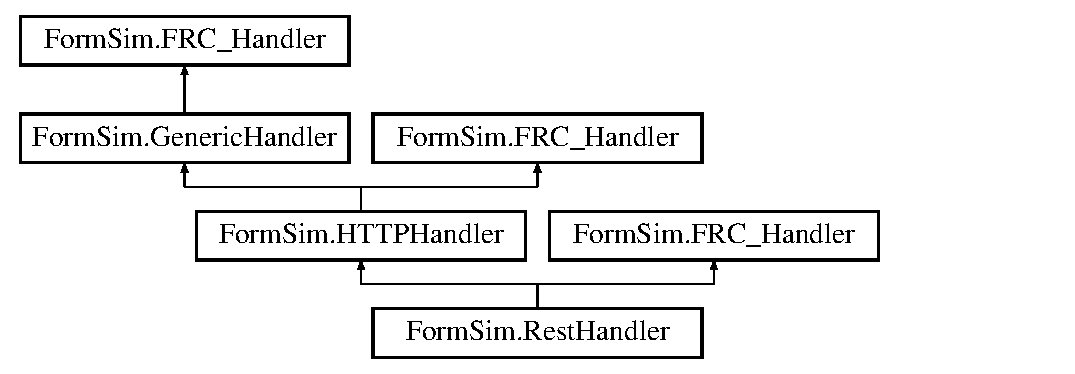
\includegraphics[height=4.000000cm]{class_form_sim_1_1_rest_handler}
\end{center}
\end{figure}
\subsection*{Public Member Functions}
\begin{DoxyCompactItemize}
\item 
\mbox{\hyperlink{class_form_sim_1_1_rest_handler_a138f2e1c350d4a14c51a0a27d36a13a8}{Rest\+Handler}} ()
\begin{DoxyCompactList}\small\item\em Default Constructor \end{DoxyCompactList}\item 
\mbox{\hyperlink{class_form_sim_1_1_rest_handler_a5a8e7dca756d6fa97fc472c1145af5cf}{Rest\+Handler}} (string \mbox{\hyperlink{class_form_sim_1_1_generic_handler_a6699d8bfc9cd305baf30ab9413b21605}{Auth\+Token}}, string \mbox{\hyperlink{class_form_sim_1_1_generic_handler_ae1d2175b140f4c600d74bbab1e22714e}{Client\+G\+U\+ID}})
\begin{DoxyCompactList}\small\item\em Optional Constructor \end{DoxyCompactList}\item 
\mbox{\hyperlink{class_form_sim_1_1_rest_handler_a01f0a6ed0453bcdf536d4062650d5bbf}{Rest\+Handler}} (string \mbox{\hyperlink{class_form_sim_1_1_generic_handler_a6699d8bfc9cd305baf30ab9413b21605}{Auth\+Token}}, string \mbox{\hyperlink{class_form_sim_1_1_generic_handler_ae1d2175b140f4c600d74bbab1e22714e}{Client\+G\+U\+ID}}, string \mbox{\hyperlink{class_form_sim_1_1_generic_handler_a12b51dea082a4d40d86829802adf073b}{I\+P\+Address}}, string \mbox{\hyperlink{class_form_sim_1_1_generic_handler_ac6492bb3e4fbe8f66c97b00bd27020c1}{Port}})
\begin{DoxyCompactList}\small\item\em Optional Constructor \end{DoxyCompactList}\item 
override async Task$<$ bool $>$ \mbox{\hyperlink{class_form_sim_1_1_rest_handler_abd5c425be2b6c9e30ca3cfc0fb696aa9}{perform\+Token\+Exchange}} ()
\begin{DoxyCompactList}\small\item\em Performs token echange over http to the R\+E\+ST interface by exchanging a client\+G\+U\+ID and Auth\+Token for an Access\+Token. \end{DoxyCompactList}\item 
async Task$<$ Dictionary$<$ string, string $>$ $>$ \mbox{\hyperlink{class_form_sim_1_1_rest_handler_a4a777189e9e16dc9970fe8f2557555db}{send\+Raw}} (string raw\+String, Dictionary$<$ string, string $>$ parameters)
\begin{DoxyCompactList}\small\item\em Allows the user to pass in a raw J\+S\+ON string, representing the P\+O\+ST body of a request. This is useful for testing results and odd requests that a vendor my supply to us. \end{DoxyCompactList}\end{DoxyCompactItemize}
\subsection*{Protected Member Functions}
\begin{DoxyCompactItemize}
\item 
override async Task$<$ Dictionary$<$ string, string $>$ $>$ \mbox{\hyperlink{class_form_sim_1_1_rest_handler_aaba7a1239d5e4e2eb63e0f24f76341d1}{perform\+Transaction}} (Dictionary$<$ string, string $>$ parameters)
\begin{DoxyCompactList}\small\item\em Performs a given F\+RC via the R\+E\+S\+Tful A\+PI, provided in the Dictionary. \end{DoxyCompactList}\end{DoxyCompactItemize}
\subsection*{Private Member Functions}
\begin{DoxyCompactItemize}
\item 
Dictionary$<$ string, string $>$ \mbox{\hyperlink{class_form_sim_1_1_rest_handler_a7c2e17caa0c591a104e9e4f9a3825f47}{void\+Transaction}} (Dictionary$<$ string, string $>$ req, Dictionary$<$ string, string $>$ res)
\begin{DoxyCompactList}\small\item\em N\+OT I\+M\+P\+L\+E\+M\+E\+N\+T\+ED -\/ Programatically voids a transaction... This may not be necessary with R\+E\+ST. \end{DoxyCompactList}\item 
String\+Content \mbox{\hyperlink{class_form_sim_1_1_rest_handler_a92192f6edc3e39d00b37dea3f8f16d93}{build\+Json\+Object}} (Dictionary$<$ string, string $>$ parameters)
\begin{DoxyCompactList}\small\item\em Builds the J\+S\+ON object from the passed dictionary using the J\+S\+O\+N\+Converter project classes. \end{DoxyCompactList}\item 
Dictionary$<$ string, string $>$ \mbox{\hyperlink{class_form_sim_1_1_rest_handler_a08ab06f861daa5acaf1aca9ea2fe8c9b}{parse\+To\+Dict}} (J\+S\+O\+N\+Converter.\+Message message)
\begin{DoxyCompactList}\small\item\em Parses the R\+E\+ST response body into a consumable Dictionary. \end{DoxyCompactList}\item 
string \mbox{\hyperlink{class_form_sim_1_1_rest_handler_ab10dcc5c39fdf95b190ed6b50d6e1ce6}{build\+Receipt}} (receipt\mbox{[}$\,$\mbox{]} receipt)
\begin{DoxyCompactList}\small\item\em Builds a receipt from the returned data that meets E\+MV requirements. \end{DoxyCompactList}\item 
string \mbox{\hyperlink{class_form_sim_1_1_rest_handler_adb1e6344809870d5b196de0c6e54a3c9}{build\+Left\+Right\+Align}} (receipt receipt\+Item)
\begin{DoxyCompactList}\small\item\em \mbox{\hyperlink{class_form_sim_1_1_helper}{Helper}} funciton that left justifies the print\+Name and right justifies the print\+Value to 30 chars wide. \end{DoxyCompactList}\item 
string \mbox{\hyperlink{class_form_sim_1_1_rest_handler_a14a4a8f672494cea85c34f23fa508464}{pick\+End\+Point}} (Dictionary$<$ string, string $>$ parameters)
\begin{DoxyCompactList}\small\item\em Picks the proper R\+E\+ST endpoint given the F\+RC. \end{DoxyCompactList}\item 
string \mbox{\hyperlink{class_form_sim_1_1_rest_handler_a205454167e8716d9c1ed0e05d6e88564}{pick\+Http\+Verb}} (Dictionary$<$ string, string $>$ parameters)
\begin{DoxyCompactList}\small\item\em Picks the proper H\+T\+TP verb (G\+ET, P\+O\+ST, D\+E\+L\+E\+TE) \end{DoxyCompactList}\item 
async Task$<$ Http\+Response\+Message $>$ \mbox{\hyperlink{class_form_sim_1_1_rest_handler_adcca9a79f3a98112628190b11fd5c7ca}{send\+G\+ET}} (Dictionary$<$ string, string $>$ parameters, string end\+Point)
\begin{DoxyCompactList}\small\item\em Sends a G\+ET request with the appropriate headers \end{DoxyCompactList}\item 
async Task$<$ Http\+Response\+Message $>$ \mbox{\hyperlink{class_form_sim_1_1_rest_handler_ae69e912f1e70c08e4a9200efcb070bf8}{send\+P\+O\+ST}} (Dictionary$<$ string, string $>$ parameters, string end\+Point, String\+Content json\+Body)
\begin{DoxyCompactList}\small\item\em Sends a P\+O\+ST request with the appropriate headers \end{DoxyCompactList}\item 
async Task$<$ Http\+Response\+Message $>$ \mbox{\hyperlink{class_form_sim_1_1_rest_handler_a6c259e23bd88dc7191327fcca06232d0}{send\+D\+E\+L\+E\+TE}} (Dictionary$<$ string, string $>$ parameters, string end\+Point)
\begin{DoxyCompactList}\small\item\em Sends a D\+E\+L\+E\+TE request with the appropriate headers \end{DoxyCompactList}\end{DoxyCompactItemize}
\subsection*{Private Attributes}
\begin{DoxyCompactItemize}
\item 
bool \mbox{\hyperlink{class_form_sim_1_1_rest_handler_ae3f4dd32629759aba164eac64175c71f}{ignore\+S\+S\+Lerrors}} = false
\item 
readonly string \mbox{\hyperlink{class_form_sim_1_1_rest_handler_a6524f2a05b5c6bbe6b3755662f86fdab}{B\+L\+O\+C\+K\+\_\+\+C\+A\+RD}} = \char`\"{}cards/block\char`\"{}
\item 
readonly string \mbox{\hyperlink{class_form_sim_1_1_rest_handler_a4338bdac23d0558177bf5df5b3639e55}{C\+A\+R\+D\+\_\+\+B\+L\+O\+C\+K\+\_\+\+S\+T\+A\+T\+US}} = \char`\"{}cards/blockstatus\char`\"{}
\item 
readonly string \mbox{\hyperlink{class_form_sim_1_1_rest_handler_a4c4b833300f1760e624cb25aedcb0cd7}{I\+D\+E\+N\+T\+I\+F\+Y\+\_\+\+C\+A\+RD}} = \char`\"{}cards/identify\char`\"{}
\item 
readonly string \mbox{\hyperlink{class_form_sim_1_1_rest_handler_a7a93675f32f8a682458f8e2d6fdf9384}{U\+N\+B\+L\+O\+C\+K\+\_\+\+C\+A\+RD}} = \char`\"{}cards/unblock\char`\"{}
\item 
readonly string \mbox{\hyperlink{class_form_sim_1_1_rest_handler_adbde7c45aab3b4a97cf1464065161dcd}{V\+E\+R\+I\+F\+Y\+\_\+\+C\+A\+RD}} = \char`\"{}cards/verify\char`\"{}
\item 
readonly string \mbox{\hyperlink{class_form_sim_1_1_rest_handler_a662385f69d094beb118184cc00d0be00}{A\+C\+C\+E\+S\+S\+\_\+\+T\+O\+K\+EN}} = \char`\"{}credentials/accesstoken\char`\"{}
\item 
readonly string \mbox{\hyperlink{class_form_sim_1_1_rest_handler_a78b7d4fdea5fe30c1f82dbe17ea2e093}{G\+E\+T\+\_\+\+D\+E\+V\+I\+C\+E\+\_\+\+I\+N\+FO}} = \char`\"{}devices/info\char`\"{}
\item 
readonly string \mbox{\hyperlink{class_form_sim_1_1_rest_handler_ad55f11f47492affe120d64685d11356f}{I\+N\+I\+T\+I\+A\+L\+I\+Z\+E\+\_\+\+R\+E\+A\+D\+E\+RS}} = \char`\"{}devices/initializereaders\char`\"{}
\item 
readonly string \mbox{\hyperlink{class_form_sim_1_1_rest_handler_a205748c1af29fb6e639c7e6ad4b78bf2}{D\+I\+S\+P\+L\+A\+Y\+\_\+\+L\+I\+N\+E\+\_\+\+I\+T\+E\+MS}} = \char`\"{}devices/lineitems\char`\"{}
\item 
readonly string \mbox{\hyperlink{class_form_sim_1_1_rest_handler_a0ed7785fca279bdb9dd7e600f71553c0}{D\+I\+S\+P\+L\+A\+Y\+\_\+\+L\+I\+N\+E\+\_\+\+I\+T\+EM}} = \char`\"{}devices/lineitems/\{item\}\char`\"{}
\item 
readonly string \mbox{\hyperlink{class_form_sim_1_1_rest_handler_a5b324ad107b08c3bdf9f5fc7814db39c}{C\+L\+E\+A\+R\+\_\+\+L\+I\+N\+E\+\_\+\+I\+T\+E\+MS}} = \char`\"{}devices/lineitems\char`\"{}
\item 
readonly string \mbox{\hyperlink{class_form_sim_1_1_rest_handler_a0d509105eef3e65ade61d66f22ee08ea}{P\+R\+I\+N\+T\+\_\+\+R\+E\+C\+E\+I\+PT}} = \char`\"{}devices/print\char`\"{}
\item 
readonly string \mbox{\hyperlink{class_form_sim_1_1_rest_handler_a072db72ff3cc31ecf995ad17c145f4b4}{P\+R\+O\+C\+E\+S\+S\+\_\+\+F\+O\+R\+MS}} = \char`\"{}devices/processform\char`\"{}
\item 
readonly string \mbox{\hyperlink{class_form_sim_1_1_rest_handler_af90c44f10cd5ead89606b811fc5ae632}{P\+R\+O\+M\+P\+T\+\_\+\+C\+O\+N\+F\+I\+R\+M\+A\+T\+I\+ON}} = \char`\"{}devices/promptconfirmation\char`\"{}
\item 
readonly string \mbox{\hyperlink{class_form_sim_1_1_rest_handler_a78226012d7df7c27ae747c20674ca706}{P\+R\+O\+M\+P\+T\+\_\+\+I\+N\+P\+UT}} = \char`\"{}devices/promptinput\char`\"{}
\item 
readonly string \mbox{\hyperlink{class_form_sim_1_1_rest_handler_ac8898c2c9addec5b05604700655dbbe9}{O\+N\+\_\+\+D\+E\+M\+A\+N\+D\+\_\+\+C\+A\+R\+D\+\_\+\+R\+E\+AD}} = \char`\"{}devices/prompts/cardread\char`\"{}
\item 
readonly string \mbox{\hyperlink{class_form_sim_1_1_rest_handler_affa0a3f303002458dbca9c7cb7dc41a7}{R\+E\+Q\+U\+E\+S\+T\+\_\+\+S\+I\+G\+N\+A\+T\+U\+RE}} = \char`\"{}devices/promptsignature\char`\"{}
\item 
readonly string \mbox{\hyperlink{class_form_sim_1_1_rest_handler_add1d76cf837e4fae753b1f625b801fc8}{D\+E\+V\+I\+C\+E\+\_\+\+R\+E\+S\+ET}} = \char`\"{}devices/reset\char`\"{}
\item 
readonly string \mbox{\hyperlink{class_form_sim_1_1_rest_handler_af1397ea44e81584c26bcb257d9ce5769}{T\+E\+R\+M\+S\+\_\+\+A\+N\+D\+\_\+\+C\+O\+N\+D\+I\+T\+I\+O\+NS}} = \char`\"{}devices/termsandconditions\char`\"{}
\item 
readonly string \mbox{\hyperlink{class_form_sim_1_1_rest_handler_a8742d658aaab597957ada79707565406}{G\+C\+\_\+\+A\+C\+T\+I\+V\+A\+TE}} = \char`\"{}giftcards/activate\char`\"{}
\item 
readonly string \mbox{\hyperlink{class_form_sim_1_1_rest_handler_a91a3268dfe038eac25dc4b294e863fd8}{G\+C\+\_\+\+B\+A\+L\+A\+N\+CE}} = \char`\"{}giftcards/balance\char`\"{}
\item 
readonly string \mbox{\hyperlink{class_form_sim_1_1_rest_handler_ab92584cf05cc40329fb2f2e4a5e8b33a}{G\+C\+\_\+\+C\+A\+N\+C\+EL}} = \char`\"{}giftcards/cancel\char`\"{}
\item 
readonly string \mbox{\hyperlink{class_form_sim_1_1_rest_handler_ae69e88368d469b455b3ae1105f819d08}{G\+C\+\_\+\+C\+A\+S\+H\+O\+UT}} = \char`\"{}giftcards/cashout\char`\"{}
\item 
readonly string \mbox{\hyperlink{class_form_sim_1_1_rest_handler_a806a27130463899de1a5a145b0a79c3d}{G\+C\+\_\+\+D\+E\+A\+C\+T\+I\+V\+A\+TE}} = \char`\"{}giftcards/deactivate\char`\"{}
\item 
readonly string \mbox{\hyperlink{class_form_sim_1_1_rest_handler_aee53bacfe8716e4f2e2365bb007218b5}{G\+C\+\_\+\+R\+E\+A\+C\+T\+I\+V\+A\+TE}} = \char`\"{}giftcards/reactivate\char`\"{}
\item 
readonly string \mbox{\hyperlink{class_form_sim_1_1_rest_handler_a4edb4283c69328bd540594c288c67fde}{G\+C\+\_\+\+R\+E\+L\+O\+AD}} = \char`\"{}giftcards/reload\char`\"{}
\item 
readonly string \mbox{\hyperlink{class_form_sim_1_1_rest_handler_ae4b8b267aea9f7d55eb821ae567d613b}{M\+E\+R\+C\+H\+A\+NT}} = \char`\"{}merchants/merchant\char`\"{}
\item 
readonly string \mbox{\hyperlink{class_form_sim_1_1_rest_handler_a7eaa83dfd3c17adad3483c6785bbae0b}{G\+E\+T\+\_\+\+N\+E\+X\+T\+\_\+\+I\+N\+V\+O\+I\+CE}} = \char`\"{}reports/batchdetails\char`\"{}
\item 
readonly string \mbox{\hyperlink{class_form_sim_1_1_rest_handler_a28d4f880c8894174f1f055abfc1f7b30}{T\+O\+T\+A\+L\+S\+\_\+\+R\+E\+P\+O\+RT}} = \char`\"{}reports/batchtotals\char`\"{}
\item 
readonly string \mbox{\hyperlink{class_form_sim_1_1_rest_handler_a8e0162fa484b58fc50eb95db9da2784f}{S\+T\+A\+T\+U\+S\+\_\+\+R\+E\+Q\+U\+E\+ST}} = \char`\"{}sessions\char`\"{}
\item 
readonly string \mbox{\hyperlink{class_form_sim_1_1_rest_handler_a2f8574a09fb25a8632817d26e6323daf}{G\+E\+T\+\_\+4\+\_\+\+W\+O\+R\+DS}} = \char`\"{}tokens/4words\char`\"{}
\item 
readonly string \mbox{\hyperlink{class_form_sim_1_1_rest_handler_a6ae5956fb935833d3e68813b786bd034}{T\+O\+K\+E\+N\+\_\+\+A\+DD}} = \char`\"{}tokens/add\char`\"{}
\item 
readonly string \mbox{\hyperlink{class_form_sim_1_1_rest_handler_a4830033d986d2f15704092cd8420f04c}{T\+O\+K\+E\+N\+\_\+\+D\+E\+L\+E\+TE}} = \char`\"{}tokens/delete\char`\"{}
\item 
readonly string \mbox{\hyperlink{class_form_sim_1_1_rest_handler_afd87386544c94ad11669b905304cda99}{T\+O\+K\+E\+N\+\_\+\+D\+U\+P\+L\+I\+C\+A\+TE}} = \char`\"{}tokens/duplicate\char`\"{}
\item 
readonly string \mbox{\hyperlink{class_form_sim_1_1_rest_handler_a33f4985d9ea1beb7984876f9e992eaae}{A\+U\+T\+H\+O\+R\+I\+Z\+A\+T\+I\+ON}} = \char`\"{}transactions/authorization\char`\"{}
\item 
readonly string \mbox{\hyperlink{class_form_sim_1_1_rest_handler_afb28bbff572b84c26be4dddf30aa0bdb}{C\+A\+P\+T\+U\+RE}} = \char`\"{}transactions/capture\char`\"{}
\item 
readonly string \mbox{\hyperlink{class_form_sim_1_1_rest_handler_abe32a138ecc549cfc16cc9846d4ca468}{C\+H\+E\+CK}} = \char`\"{}transactions/check\char`\"{}
\item 
readonly string \mbox{\hyperlink{class_form_sim_1_1_rest_handler_adee0030a983637e00e79cda3b5a1dfb6}{I\+N\+V\+O\+I\+CE}} = \char`\"{}transactions/invoice\char`\"{}
\item 
readonly string \mbox{\hyperlink{class_form_sim_1_1_rest_handler_a11a3ee0812c27c88988615f24ecb25dc}{M\+A\+N\+U\+A\+L\+\_\+\+A\+U\+T\+H\+O\+R\+I\+Z\+A\+T\+I\+ON}} = \char`\"{}transactions/manualauthorization\char`\"{}
\item 
readonly string \mbox{\hyperlink{class_form_sim_1_1_rest_handler_a8c04225218b1ea8873b6a7e4635147bf}{M\+A\+N\+U\+A\+L\+\_\+\+S\+A\+LE}} = \char`\"{}transactions/manualsale\char`\"{}
\item 
readonly string \mbox{\hyperlink{class_form_sim_1_1_rest_handler_a1210812ce0844c10de03694bcffb464c}{R\+E\+F\+U\+ND}} = \char`\"{}transactions/refund\char`\"{}
\item 
readonly string \mbox{\hyperlink{class_form_sim_1_1_rest_handler_aa120f59ea2b44fc2ad0e2d95ab9dd18f}{S\+A\+LE}} = \char`\"{}transactions/sale\char`\"{}
\item 
readonly string \mbox{\hyperlink{class_form_sim_1_1_rest_handler_a54fcdefde2b8518a8ce326ca362cf09d}{S\+I\+G\+N\+A\+T\+U\+RE}} = \char`\"{}transactions/signature\char`\"{}
\item 
readonly string \mbox{\hyperlink{class_form_sim_1_1_rest_handler_af5d7a5c25979759bf51b7ede862718b2}{S\+E\+S\+S\+I\+ON}} = \char`\"{}status\char`\"{}
\item 
string \mbox{\hyperlink{class_form_sim_1_1_rest_handler_a2b2da7000557616345192ffd589b4e16}{json\+\_\+out}}
\item 
bool \mbox{\hyperlink{class_form_sim_1_1_rest_handler_ad2cd92751f0b8f3317205b32d1ba401d}{headers\+Set}}
\end{DoxyCompactItemize}
\subsection*{Additional Inherited Members}


\subsection{Detailed Description}
The \mbox{\hyperlink{class_form_sim_1_1_rest_handler}{Rest\+Handler}} class is designed to handle F\+RC\textquotesingle{}s over the H\+T\+TP protocol to the R\+E\+S\+Tful A\+PI. This implementation uses J\+S\+ON as the payload format, so serializing and deserializing are handled here. It also acts as a translation layer between the required Dictionary of strings, and the returned J\+S\+ON from the R\+E\+ST interface. 



\subsection{Constructor \& Destructor Documentation}
\mbox{\Hypertarget{class_form_sim_1_1_rest_handler_a138f2e1c350d4a14c51a0a27d36a13a8}\label{class_form_sim_1_1_rest_handler_a138f2e1c350d4a14c51a0a27d36a13a8}} 
\index{Form\+Sim\+::\+Rest\+Handler@{Form\+Sim\+::\+Rest\+Handler}!Rest\+Handler@{Rest\+Handler}}
\index{Rest\+Handler@{Rest\+Handler}!Form\+Sim\+::\+Rest\+Handler@{Form\+Sim\+::\+Rest\+Handler}}
\subsubsection{\texorpdfstring{Rest\+Handler()}{RestHandler()}\hspace{0.1cm}{\footnotesize\ttfamily [1/3]}}
{\footnotesize\ttfamily Form\+Sim.\+Rest\+Handler.\+Rest\+Handler (\begin{DoxyParamCaption}{ }\end{DoxyParamCaption})\hspace{0.3cm}{\ttfamily [inline]}}



Default Constructor 

\mbox{\Hypertarget{class_form_sim_1_1_rest_handler_a5a8e7dca756d6fa97fc472c1145af5cf}\label{class_form_sim_1_1_rest_handler_a5a8e7dca756d6fa97fc472c1145af5cf}} 
\index{Form\+Sim\+::\+Rest\+Handler@{Form\+Sim\+::\+Rest\+Handler}!Rest\+Handler@{Rest\+Handler}}
\index{Rest\+Handler@{Rest\+Handler}!Form\+Sim\+::\+Rest\+Handler@{Form\+Sim\+::\+Rest\+Handler}}
\subsubsection{\texorpdfstring{Rest\+Handler()}{RestHandler()}\hspace{0.1cm}{\footnotesize\ttfamily [2/3]}}
{\footnotesize\ttfamily Form\+Sim.\+Rest\+Handler.\+Rest\+Handler (\begin{DoxyParamCaption}\item[{string}]{Auth\+Token,  }\item[{string}]{Client\+G\+U\+ID }\end{DoxyParamCaption})\hspace{0.3cm}{\ttfamily [inline]}}



Optional Constructor 


\begin{DoxyParams}{Parameters}
{\em Auth\+Token} & The Auth\+Token provided by Shift4 for a given M\+ID.\\
\hline
{\em Client\+G\+U\+ID} & The Client\+G\+U\+ID assigned by Shift4 for a given interface.\\
\hline
\end{DoxyParams}
\mbox{\Hypertarget{class_form_sim_1_1_rest_handler_a01f0a6ed0453bcdf536d4062650d5bbf}\label{class_form_sim_1_1_rest_handler_a01f0a6ed0453bcdf536d4062650d5bbf}} 
\index{Form\+Sim\+::\+Rest\+Handler@{Form\+Sim\+::\+Rest\+Handler}!Rest\+Handler@{Rest\+Handler}}
\index{Rest\+Handler@{Rest\+Handler}!Form\+Sim\+::\+Rest\+Handler@{Form\+Sim\+::\+Rest\+Handler}}
\subsubsection{\texorpdfstring{Rest\+Handler()}{RestHandler()}\hspace{0.1cm}{\footnotesize\ttfamily [3/3]}}
{\footnotesize\ttfamily Form\+Sim.\+Rest\+Handler.\+Rest\+Handler (\begin{DoxyParamCaption}\item[{string}]{Auth\+Token,  }\item[{string}]{Client\+G\+U\+ID,  }\item[{string}]{I\+P\+Address,  }\item[{string}]{Port }\end{DoxyParamCaption})\hspace{0.3cm}{\ttfamily [inline]}}



Optional Constructor 


\begin{DoxyParams}{Parameters}
{\em Auth\+Token} & The Auth\+Token provided by Shift4 for a given M\+ID.\\
\hline
{\em Client\+G\+U\+ID} & The Client\+G\+U\+ID assigned by Shift4 for a given interface.\\
\hline
{\em I\+P\+Address} & The IP address, or base U\+RL of the Shift4 U\+TG.\\
\hline
{\em Port} & The port over which to communicate.\\
\hline
\end{DoxyParams}


\subsection{Member Function Documentation}
\mbox{\Hypertarget{class_form_sim_1_1_rest_handler_a92192f6edc3e39d00b37dea3f8f16d93}\label{class_form_sim_1_1_rest_handler_a92192f6edc3e39d00b37dea3f8f16d93}} 
\index{Form\+Sim\+::\+Rest\+Handler@{Form\+Sim\+::\+Rest\+Handler}!build\+Json\+Object@{build\+Json\+Object}}
\index{build\+Json\+Object@{build\+Json\+Object}!Form\+Sim\+::\+Rest\+Handler@{Form\+Sim\+::\+Rest\+Handler}}
\subsubsection{\texorpdfstring{build\+Json\+Object()}{buildJsonObject()}}
{\footnotesize\ttfamily String\+Content Form\+Sim.\+Rest\+Handler.\+build\+Json\+Object (\begin{DoxyParamCaption}\item[{Dictionary$<$ string, string $>$}]{parameters }\end{DoxyParamCaption})\hspace{0.3cm}{\ttfamily [inline]}, {\ttfamily [private]}}



Builds the J\+S\+ON object from the passed dictionary using the J\+S\+O\+N\+Converter project classes. 

\mbox{\Hypertarget{class_form_sim_1_1_rest_handler_adb1e6344809870d5b196de0c6e54a3c9}\label{class_form_sim_1_1_rest_handler_adb1e6344809870d5b196de0c6e54a3c9}} 
\index{Form\+Sim\+::\+Rest\+Handler@{Form\+Sim\+::\+Rest\+Handler}!build\+Left\+Right\+Align@{build\+Left\+Right\+Align}}
\index{build\+Left\+Right\+Align@{build\+Left\+Right\+Align}!Form\+Sim\+::\+Rest\+Handler@{Form\+Sim\+::\+Rest\+Handler}}
\subsubsection{\texorpdfstring{build\+Left\+Right\+Align()}{buildLeftRightAlign()}}
{\footnotesize\ttfamily string Form\+Sim.\+Rest\+Handler.\+build\+Left\+Right\+Align (\begin{DoxyParamCaption}\item[{receipt}]{receipt\+Item }\end{DoxyParamCaption})\hspace{0.3cm}{\ttfamily [inline]}, {\ttfamily [private]}}



\mbox{\hyperlink{class_form_sim_1_1_helper}{Helper}} funciton that left justifies the print\+Name and right justifies the print\+Value to 30 chars wide. 


\begin{DoxyParams}{Parameters}
{\em receipt\+Item} & A single line item for the receipt.\\
\hline
\end{DoxyParams}
\begin{DoxyReturn}{Returns}
The properly spaced string representation of the line item.
\end{DoxyReturn}
\mbox{\Hypertarget{class_form_sim_1_1_rest_handler_ab10dcc5c39fdf95b190ed6b50d6e1ce6}\label{class_form_sim_1_1_rest_handler_ab10dcc5c39fdf95b190ed6b50d6e1ce6}} 
\index{Form\+Sim\+::\+Rest\+Handler@{Form\+Sim\+::\+Rest\+Handler}!build\+Receipt@{build\+Receipt}}
\index{build\+Receipt@{build\+Receipt}!Form\+Sim\+::\+Rest\+Handler@{Form\+Sim\+::\+Rest\+Handler}}
\subsubsection{\texorpdfstring{build\+Receipt()}{buildReceipt()}}
{\footnotesize\ttfamily string Form\+Sim.\+Rest\+Handler.\+build\+Receipt (\begin{DoxyParamCaption}\item[{receipt \mbox{[}$\,$\mbox{]}}]{receipt }\end{DoxyParamCaption})\hspace{0.3cm}{\ttfamily [inline]}, {\ttfamily [private]}}



Builds a receipt from the returned data that meets E\+MV requirements. 


\begin{DoxyParams}{Parameters}
{\em receipt} & An array of receipt items returned from Shift4.\\
\hline
\end{DoxyParams}
\begin{DoxyReturn}{Returns}
A string representation of the receipt text. The receipt is left justified and 30 chars wide.
\end{DoxyReturn}
\mbox{\Hypertarget{class_form_sim_1_1_rest_handler_a08ab06f861daa5acaf1aca9ea2fe8c9b}\label{class_form_sim_1_1_rest_handler_a08ab06f861daa5acaf1aca9ea2fe8c9b}} 
\index{Form\+Sim\+::\+Rest\+Handler@{Form\+Sim\+::\+Rest\+Handler}!parse\+To\+Dict@{parse\+To\+Dict}}
\index{parse\+To\+Dict@{parse\+To\+Dict}!Form\+Sim\+::\+Rest\+Handler@{Form\+Sim\+::\+Rest\+Handler}}
\subsubsection{\texorpdfstring{parse\+To\+Dict()}{parseToDict()}}
{\footnotesize\ttfamily Dictionary$<$string, string$>$ Form\+Sim.\+Rest\+Handler.\+parse\+To\+Dict (\begin{DoxyParamCaption}\item[{J\+S\+O\+N\+Converter.\+Message}]{message }\end{DoxyParamCaption})\hspace{0.3cm}{\ttfamily [inline]}, {\ttfamily [private]}}



Parses the R\+E\+ST response body into a consumable Dictionary. 


\begin{DoxyParams}{Parameters}
{\em message} & The top level J\+S\+ON Object sent or returned to Shift4\textquotesingle{}s R\+E\+S\+Tful A\+PI.\\
\hline
\end{DoxyParams}
\begin{DoxyReturn}{Returns}
A Dictionary representation of a response or request body from a J\+S\+ON Message Object.
\end{DoxyReturn}
\mbox{\Hypertarget{class_form_sim_1_1_rest_handler_abd5c425be2b6c9e30ca3cfc0fb696aa9}\label{class_form_sim_1_1_rest_handler_abd5c425be2b6c9e30ca3cfc0fb696aa9}} 
\index{Form\+Sim\+::\+Rest\+Handler@{Form\+Sim\+::\+Rest\+Handler}!perform\+Token\+Exchange@{perform\+Token\+Exchange}}
\index{perform\+Token\+Exchange@{perform\+Token\+Exchange}!Form\+Sim\+::\+Rest\+Handler@{Form\+Sim\+::\+Rest\+Handler}}
\subsubsection{\texorpdfstring{perform\+Token\+Exchange()}{performTokenExchange()}}
{\footnotesize\ttfamily override async Task$<$bool$>$ Form\+Sim.\+Rest\+Handler.\+perform\+Token\+Exchange (\begin{DoxyParamCaption}{ }\end{DoxyParamCaption})\hspace{0.3cm}{\ttfamily [inline]}}



Performs token echange over http to the R\+E\+ST interface by exchanging a client\+G\+U\+ID and Auth\+Token for an Access\+Token. 



Implements \mbox{\hyperlink{interface_form_sim_1_1_f_r_c___handler_a32c299d3cb3cdd6c444e76b3671af1b4}{Form\+Sim.\+F\+R\+C\+\_\+\+Handler}}.

\mbox{\Hypertarget{class_form_sim_1_1_rest_handler_aaba7a1239d5e4e2eb63e0f24f76341d1}\label{class_form_sim_1_1_rest_handler_aaba7a1239d5e4e2eb63e0f24f76341d1}} 
\index{Form\+Sim\+::\+Rest\+Handler@{Form\+Sim\+::\+Rest\+Handler}!perform\+Transaction@{perform\+Transaction}}
\index{perform\+Transaction@{perform\+Transaction}!Form\+Sim\+::\+Rest\+Handler@{Form\+Sim\+::\+Rest\+Handler}}
\subsubsection{\texorpdfstring{perform\+Transaction()}{performTransaction()}}
{\footnotesize\ttfamily override async Task$<$Dictionary$<$string, string$>$ $>$ Form\+Sim.\+Rest\+Handler.\+perform\+Transaction (\begin{DoxyParamCaption}\item[{Dictionary$<$ string, string $>$}]{parameters }\end{DoxyParamCaption})\hspace{0.3cm}{\ttfamily [inline]}, {\ttfamily [protected]}, {\ttfamily [virtual]}}



Performs a given F\+RC via the R\+E\+S\+Tful A\+PI, provided in the Dictionary. 


\begin{DoxyParams}{Parameters}
{\em parameters} & See \mbox{\hyperlink{interface_form_sim_1_1_f_r_c___handler_a2a2a8a776e774e5f8b5e2b7e623a26a6}{F\+R\+C\+\_\+\+Handler.\+start(\+Dictionary$<$string, string$>$)}}\\
\hline
\end{DoxyParams}
\begin{DoxyReturn}{Returns}
A thread with the results of the transaction in a dictionary.
\end{DoxyReturn}


Reimplemented from \mbox{\hyperlink{class_form_sim_1_1_h_t_t_p_handler_a1b87e232c94cf390f7a9656744006639}{Form\+Sim.\+H\+T\+T\+P\+Handler}}.

\mbox{\Hypertarget{class_form_sim_1_1_rest_handler_a14a4a8f672494cea85c34f23fa508464}\label{class_form_sim_1_1_rest_handler_a14a4a8f672494cea85c34f23fa508464}} 
\index{Form\+Sim\+::\+Rest\+Handler@{Form\+Sim\+::\+Rest\+Handler}!pick\+End\+Point@{pick\+End\+Point}}
\index{pick\+End\+Point@{pick\+End\+Point}!Form\+Sim\+::\+Rest\+Handler@{Form\+Sim\+::\+Rest\+Handler}}
\subsubsection{\texorpdfstring{pick\+End\+Point()}{pickEndPoint()}}
{\footnotesize\ttfamily string Form\+Sim.\+Rest\+Handler.\+pick\+End\+Point (\begin{DoxyParamCaption}\item[{Dictionary$<$ string, string $>$}]{parameters }\end{DoxyParamCaption})\hspace{0.3cm}{\ttfamily [inline]}, {\ttfamily [private]}}



Picks the proper R\+E\+ST endpoint given the F\+RC. 


\begin{DoxyParams}{Parameters}
{\em parameters} & A Dictionary of the request fields that will be sent.\\
\hline
\end{DoxyParams}
\begin{DoxyReturn}{Returns}
The string representaiton of the U\+RI for the given F\+RC.
\end{DoxyReturn}
\mbox{\Hypertarget{class_form_sim_1_1_rest_handler_a205454167e8716d9c1ed0e05d6e88564}\label{class_form_sim_1_1_rest_handler_a205454167e8716d9c1ed0e05d6e88564}} 
\index{Form\+Sim\+::\+Rest\+Handler@{Form\+Sim\+::\+Rest\+Handler}!pick\+Http\+Verb@{pick\+Http\+Verb}}
\index{pick\+Http\+Verb@{pick\+Http\+Verb}!Form\+Sim\+::\+Rest\+Handler@{Form\+Sim\+::\+Rest\+Handler}}
\subsubsection{\texorpdfstring{pick\+Http\+Verb()}{pickHttpVerb()}}
{\footnotesize\ttfamily string Form\+Sim.\+Rest\+Handler.\+pick\+Http\+Verb (\begin{DoxyParamCaption}\item[{Dictionary$<$ string, string $>$}]{parameters }\end{DoxyParamCaption})\hspace{0.3cm}{\ttfamily [inline]}, {\ttfamily [private]}}



Picks the proper H\+T\+TP verb (G\+ET, P\+O\+ST, D\+E\+L\+E\+TE) 


\begin{DoxyParams}{Parameters}
{\em parameters} & A Dictionary of the request fields that will be sent.\\
\hline
\end{DoxyParams}
\begin{DoxyReturn}{Returns}
The string representation of the H\+T\+TP verb to use in the request.
\end{DoxyReturn}
\mbox{\Hypertarget{class_form_sim_1_1_rest_handler_a6c259e23bd88dc7191327fcca06232d0}\label{class_form_sim_1_1_rest_handler_a6c259e23bd88dc7191327fcca06232d0}} 
\index{Form\+Sim\+::\+Rest\+Handler@{Form\+Sim\+::\+Rest\+Handler}!send\+D\+E\+L\+E\+TE@{send\+D\+E\+L\+E\+TE}}
\index{send\+D\+E\+L\+E\+TE@{send\+D\+E\+L\+E\+TE}!Form\+Sim\+::\+Rest\+Handler@{Form\+Sim\+::\+Rest\+Handler}}
\subsubsection{\texorpdfstring{send\+D\+E\+L\+E\+T\+E()}{sendDELETE()}}
{\footnotesize\ttfamily async Task$<$Http\+Response\+Message$>$ Form\+Sim.\+Rest\+Handler.\+send\+D\+E\+L\+E\+TE (\begin{DoxyParamCaption}\item[{Dictionary$<$ string, string $>$}]{parameters,  }\item[{string}]{end\+Point }\end{DoxyParamCaption})\hspace{0.3cm}{\ttfamily [inline]}, {\ttfamily [private]}}



Sends a D\+E\+L\+E\+TE request with the appropriate headers 


\begin{DoxyParams}{Parameters}
{\em parameters} & A Dictionary of the request fields that will be sent.\\
\hline
{\em end\+Point} & The endpoint the D\+E\+L\+E\+TE request is supposed to hit.\\
\hline
\end{DoxyParams}
\begin{DoxyReturn}{Returns}
A thread with the Http\+Response\+Message returned from the endpoint.
\end{DoxyReturn}
\mbox{\Hypertarget{class_form_sim_1_1_rest_handler_adcca9a79f3a98112628190b11fd5c7ca}\label{class_form_sim_1_1_rest_handler_adcca9a79f3a98112628190b11fd5c7ca}} 
\index{Form\+Sim\+::\+Rest\+Handler@{Form\+Sim\+::\+Rest\+Handler}!send\+G\+ET@{send\+G\+ET}}
\index{send\+G\+ET@{send\+G\+ET}!Form\+Sim\+::\+Rest\+Handler@{Form\+Sim\+::\+Rest\+Handler}}
\subsubsection{\texorpdfstring{send\+G\+E\+T()}{sendGET()}}
{\footnotesize\ttfamily async Task$<$Http\+Response\+Message$>$ Form\+Sim.\+Rest\+Handler.\+send\+G\+ET (\begin{DoxyParamCaption}\item[{Dictionary$<$ string, string $>$}]{parameters,  }\item[{string}]{end\+Point }\end{DoxyParamCaption})\hspace{0.3cm}{\ttfamily [inline]}, {\ttfamily [private]}}



Sends a G\+ET request with the appropriate headers 


\begin{DoxyParams}{Parameters}
{\em parameters} & A Dictionary of the request fields that will be sent.\\
\hline
{\em end\+Point} & The endpoint the G\+ET request is supposed to hit.\\
\hline
\end{DoxyParams}
\begin{DoxyReturn}{Returns}
A thread with the Http\+Response\+Message returned from the endpoint.
\end{DoxyReturn}
\mbox{\Hypertarget{class_form_sim_1_1_rest_handler_ae69e912f1e70c08e4a9200efcb070bf8}\label{class_form_sim_1_1_rest_handler_ae69e912f1e70c08e4a9200efcb070bf8}} 
\index{Form\+Sim\+::\+Rest\+Handler@{Form\+Sim\+::\+Rest\+Handler}!send\+P\+O\+ST@{send\+P\+O\+ST}}
\index{send\+P\+O\+ST@{send\+P\+O\+ST}!Form\+Sim\+::\+Rest\+Handler@{Form\+Sim\+::\+Rest\+Handler}}
\subsubsection{\texorpdfstring{send\+P\+O\+S\+T()}{sendPOST()}}
{\footnotesize\ttfamily async Task$<$Http\+Response\+Message$>$ Form\+Sim.\+Rest\+Handler.\+send\+P\+O\+ST (\begin{DoxyParamCaption}\item[{Dictionary$<$ string, string $>$}]{parameters,  }\item[{string}]{end\+Point,  }\item[{String\+Content}]{json\+Body }\end{DoxyParamCaption})\hspace{0.3cm}{\ttfamily [inline]}, {\ttfamily [private]}}



Sends a P\+O\+ST request with the appropriate headers 


\begin{DoxyParams}{Parameters}
{\em parameters} & A Dictionary of the request fields that will be sent.\\
\hline
{\em end\+Point} & The endpoint the P\+O\+ST request is supposed to hit.\\
\hline
{\em json\+Body} & The J\+S\+ON body of the P\+O\+ST request.\\
\hline
\end{DoxyParams}
\begin{DoxyReturn}{Returns}
A thread with the Http\+Response\+Message returned from the endpoint.
\end{DoxyReturn}
\mbox{\Hypertarget{class_form_sim_1_1_rest_handler_a4a777189e9e16dc9970fe8f2557555db}\label{class_form_sim_1_1_rest_handler_a4a777189e9e16dc9970fe8f2557555db}} 
\index{Form\+Sim\+::\+Rest\+Handler@{Form\+Sim\+::\+Rest\+Handler}!send\+Raw@{send\+Raw}}
\index{send\+Raw@{send\+Raw}!Form\+Sim\+::\+Rest\+Handler@{Form\+Sim\+::\+Rest\+Handler}}
\subsubsection{\texorpdfstring{send\+Raw()}{sendRaw()}}
{\footnotesize\ttfamily async Task$<$Dictionary$<$string, string$>$ $>$ Form\+Sim.\+Rest\+Handler.\+send\+Raw (\begin{DoxyParamCaption}\item[{string}]{raw\+String,  }\item[{Dictionary$<$ string, string $>$}]{parameters }\end{DoxyParamCaption})\hspace{0.3cm}{\ttfamily [inline]}}



Allows the user to pass in a raw J\+S\+ON string, representing the P\+O\+ST body of a request. This is useful for testing results and odd requests that a vendor my supply to us. 


\begin{DoxyParams}{Parameters}
{\em raw\+String} & The J\+S\+ON body of a post request.\\
\hline
{\em parameters} & A Dictionary with just enough fields to indicate what endpoint to use.\\
\hline
\end{DoxyParams}
\begin{DoxyReturn}{Returns}
A thread with a Dictionary of the results of the \char`\"{}raw\char`\"{} request.
\end{DoxyReturn}


Implements \mbox{\hyperlink{interface_form_sim_1_1_f_r_c___handler_ad4b9146b6142d1d6ded15e5de4ed4675}{Form\+Sim.\+F\+R\+C\+\_\+\+Handler}}.

\mbox{\Hypertarget{class_form_sim_1_1_rest_handler_a7c2e17caa0c591a104e9e4f9a3825f47}\label{class_form_sim_1_1_rest_handler_a7c2e17caa0c591a104e9e4f9a3825f47}} 
\index{Form\+Sim\+::\+Rest\+Handler@{Form\+Sim\+::\+Rest\+Handler}!void\+Transaction@{void\+Transaction}}
\index{void\+Transaction@{void\+Transaction}!Form\+Sim\+::\+Rest\+Handler@{Form\+Sim\+::\+Rest\+Handler}}
\subsubsection{\texorpdfstring{void\+Transaction()}{voidTransaction()}}
{\footnotesize\ttfamily Dictionary$<$string, string$>$ Form\+Sim.\+Rest\+Handler.\+void\+Transaction (\begin{DoxyParamCaption}\item[{Dictionary$<$ string, string $>$}]{req,  }\item[{Dictionary$<$ string, string $>$}]{res }\end{DoxyParamCaption})\hspace{0.3cm}{\ttfamily [inline]}, {\ttfamily [private]}}



N\+OT I\+M\+P\+L\+E\+M\+E\+N\+T\+ED -\/ Programatically voids a transaction... This may not be necessary with R\+E\+ST. 


\begin{DoxyParams}{Parameters}
{\em req} & A Dictionary that represent the fields that were sent in the initial request.\\
\hline
{\em res} & A Dictionary that represents the fields that were returned from the initial requst.\\
\hline
\end{DoxyParams}


\subsection{Member Data Documentation}
\mbox{\Hypertarget{class_form_sim_1_1_rest_handler_a662385f69d094beb118184cc00d0be00}\label{class_form_sim_1_1_rest_handler_a662385f69d094beb118184cc00d0be00}} 
\index{Form\+Sim\+::\+Rest\+Handler@{Form\+Sim\+::\+Rest\+Handler}!A\+C\+C\+E\+S\+S\+\_\+\+T\+O\+K\+EN@{A\+C\+C\+E\+S\+S\+\_\+\+T\+O\+K\+EN}}
\index{A\+C\+C\+E\+S\+S\+\_\+\+T\+O\+K\+EN@{A\+C\+C\+E\+S\+S\+\_\+\+T\+O\+K\+EN}!Form\+Sim\+::\+Rest\+Handler@{Form\+Sim\+::\+Rest\+Handler}}
\subsubsection{\texorpdfstring{A\+C\+C\+E\+S\+S\+\_\+\+T\+O\+K\+EN}{ACCESS\_TOKEN}}
{\footnotesize\ttfamily readonly string Form\+Sim.\+Rest\+Handler.\+A\+C\+C\+E\+S\+S\+\_\+\+T\+O\+K\+EN = \char`\"{}credentials/accesstoken\char`\"{}\hspace{0.3cm}{\ttfamily [private]}}

\mbox{\Hypertarget{class_form_sim_1_1_rest_handler_a33f4985d9ea1beb7984876f9e992eaae}\label{class_form_sim_1_1_rest_handler_a33f4985d9ea1beb7984876f9e992eaae}} 
\index{Form\+Sim\+::\+Rest\+Handler@{Form\+Sim\+::\+Rest\+Handler}!A\+U\+T\+H\+O\+R\+I\+Z\+A\+T\+I\+ON@{A\+U\+T\+H\+O\+R\+I\+Z\+A\+T\+I\+ON}}
\index{A\+U\+T\+H\+O\+R\+I\+Z\+A\+T\+I\+ON@{A\+U\+T\+H\+O\+R\+I\+Z\+A\+T\+I\+ON}!Form\+Sim\+::\+Rest\+Handler@{Form\+Sim\+::\+Rest\+Handler}}
\subsubsection{\texorpdfstring{A\+U\+T\+H\+O\+R\+I\+Z\+A\+T\+I\+ON}{AUTHORIZATION}}
{\footnotesize\ttfamily readonly string Form\+Sim.\+Rest\+Handler.\+A\+U\+T\+H\+O\+R\+I\+Z\+A\+T\+I\+ON = \char`\"{}transactions/authorization\char`\"{}\hspace{0.3cm}{\ttfamily [private]}}

\mbox{\Hypertarget{class_form_sim_1_1_rest_handler_a6524f2a05b5c6bbe6b3755662f86fdab}\label{class_form_sim_1_1_rest_handler_a6524f2a05b5c6bbe6b3755662f86fdab}} 
\index{Form\+Sim\+::\+Rest\+Handler@{Form\+Sim\+::\+Rest\+Handler}!B\+L\+O\+C\+K\+\_\+\+C\+A\+RD@{B\+L\+O\+C\+K\+\_\+\+C\+A\+RD}}
\index{B\+L\+O\+C\+K\+\_\+\+C\+A\+RD@{B\+L\+O\+C\+K\+\_\+\+C\+A\+RD}!Form\+Sim\+::\+Rest\+Handler@{Form\+Sim\+::\+Rest\+Handler}}
\subsubsection{\texorpdfstring{B\+L\+O\+C\+K\+\_\+\+C\+A\+RD}{BLOCK\_CARD}}
{\footnotesize\ttfamily readonly string Form\+Sim.\+Rest\+Handler.\+B\+L\+O\+C\+K\+\_\+\+C\+A\+RD = \char`\"{}cards/block\char`\"{}\hspace{0.3cm}{\ttfamily [private]}}

\mbox{\Hypertarget{class_form_sim_1_1_rest_handler_afb28bbff572b84c26be4dddf30aa0bdb}\label{class_form_sim_1_1_rest_handler_afb28bbff572b84c26be4dddf30aa0bdb}} 
\index{Form\+Sim\+::\+Rest\+Handler@{Form\+Sim\+::\+Rest\+Handler}!C\+A\+P\+T\+U\+RE@{C\+A\+P\+T\+U\+RE}}
\index{C\+A\+P\+T\+U\+RE@{C\+A\+P\+T\+U\+RE}!Form\+Sim\+::\+Rest\+Handler@{Form\+Sim\+::\+Rest\+Handler}}
\subsubsection{\texorpdfstring{C\+A\+P\+T\+U\+RE}{CAPTURE}}
{\footnotesize\ttfamily readonly string Form\+Sim.\+Rest\+Handler.\+C\+A\+P\+T\+U\+RE = \char`\"{}transactions/capture\char`\"{}\hspace{0.3cm}{\ttfamily [private]}}

\mbox{\Hypertarget{class_form_sim_1_1_rest_handler_a4338bdac23d0558177bf5df5b3639e55}\label{class_form_sim_1_1_rest_handler_a4338bdac23d0558177bf5df5b3639e55}} 
\index{Form\+Sim\+::\+Rest\+Handler@{Form\+Sim\+::\+Rest\+Handler}!C\+A\+R\+D\+\_\+\+B\+L\+O\+C\+K\+\_\+\+S\+T\+A\+T\+US@{C\+A\+R\+D\+\_\+\+B\+L\+O\+C\+K\+\_\+\+S\+T\+A\+T\+US}}
\index{C\+A\+R\+D\+\_\+\+B\+L\+O\+C\+K\+\_\+\+S\+T\+A\+T\+US@{C\+A\+R\+D\+\_\+\+B\+L\+O\+C\+K\+\_\+\+S\+T\+A\+T\+US}!Form\+Sim\+::\+Rest\+Handler@{Form\+Sim\+::\+Rest\+Handler}}
\subsubsection{\texorpdfstring{C\+A\+R\+D\+\_\+\+B\+L\+O\+C\+K\+\_\+\+S\+T\+A\+T\+US}{CARD\_BLOCK\_STATUS}}
{\footnotesize\ttfamily readonly string Form\+Sim.\+Rest\+Handler.\+C\+A\+R\+D\+\_\+\+B\+L\+O\+C\+K\+\_\+\+S\+T\+A\+T\+US = \char`\"{}cards/blockstatus\char`\"{}\hspace{0.3cm}{\ttfamily [private]}}

\mbox{\Hypertarget{class_form_sim_1_1_rest_handler_abe32a138ecc549cfc16cc9846d4ca468}\label{class_form_sim_1_1_rest_handler_abe32a138ecc549cfc16cc9846d4ca468}} 
\index{Form\+Sim\+::\+Rest\+Handler@{Form\+Sim\+::\+Rest\+Handler}!C\+H\+E\+CK@{C\+H\+E\+CK}}
\index{C\+H\+E\+CK@{C\+H\+E\+CK}!Form\+Sim\+::\+Rest\+Handler@{Form\+Sim\+::\+Rest\+Handler}}
\subsubsection{\texorpdfstring{C\+H\+E\+CK}{CHECK}}
{\footnotesize\ttfamily readonly string Form\+Sim.\+Rest\+Handler.\+C\+H\+E\+CK = \char`\"{}transactions/check\char`\"{}\hspace{0.3cm}{\ttfamily [private]}}

\mbox{\Hypertarget{class_form_sim_1_1_rest_handler_a5b324ad107b08c3bdf9f5fc7814db39c}\label{class_form_sim_1_1_rest_handler_a5b324ad107b08c3bdf9f5fc7814db39c}} 
\index{Form\+Sim\+::\+Rest\+Handler@{Form\+Sim\+::\+Rest\+Handler}!C\+L\+E\+A\+R\+\_\+\+L\+I\+N\+E\+\_\+\+I\+T\+E\+MS@{C\+L\+E\+A\+R\+\_\+\+L\+I\+N\+E\+\_\+\+I\+T\+E\+MS}}
\index{C\+L\+E\+A\+R\+\_\+\+L\+I\+N\+E\+\_\+\+I\+T\+E\+MS@{C\+L\+E\+A\+R\+\_\+\+L\+I\+N\+E\+\_\+\+I\+T\+E\+MS}!Form\+Sim\+::\+Rest\+Handler@{Form\+Sim\+::\+Rest\+Handler}}
\subsubsection{\texorpdfstring{C\+L\+E\+A\+R\+\_\+\+L\+I\+N\+E\+\_\+\+I\+T\+E\+MS}{CLEAR\_LINE\_ITEMS}}
{\footnotesize\ttfamily readonly string Form\+Sim.\+Rest\+Handler.\+C\+L\+E\+A\+R\+\_\+\+L\+I\+N\+E\+\_\+\+I\+T\+E\+MS = \char`\"{}devices/lineitems\char`\"{}\hspace{0.3cm}{\ttfamily [private]}}

\mbox{\Hypertarget{class_form_sim_1_1_rest_handler_add1d76cf837e4fae753b1f625b801fc8}\label{class_form_sim_1_1_rest_handler_add1d76cf837e4fae753b1f625b801fc8}} 
\index{Form\+Sim\+::\+Rest\+Handler@{Form\+Sim\+::\+Rest\+Handler}!D\+E\+V\+I\+C\+E\+\_\+\+R\+E\+S\+ET@{D\+E\+V\+I\+C\+E\+\_\+\+R\+E\+S\+ET}}
\index{D\+E\+V\+I\+C\+E\+\_\+\+R\+E\+S\+ET@{D\+E\+V\+I\+C\+E\+\_\+\+R\+E\+S\+ET}!Form\+Sim\+::\+Rest\+Handler@{Form\+Sim\+::\+Rest\+Handler}}
\subsubsection{\texorpdfstring{D\+E\+V\+I\+C\+E\+\_\+\+R\+E\+S\+ET}{DEVICE\_RESET}}
{\footnotesize\ttfamily readonly string Form\+Sim.\+Rest\+Handler.\+D\+E\+V\+I\+C\+E\+\_\+\+R\+E\+S\+ET = \char`\"{}devices/reset\char`\"{}\hspace{0.3cm}{\ttfamily [private]}}

\mbox{\Hypertarget{class_form_sim_1_1_rest_handler_a0ed7785fca279bdb9dd7e600f71553c0}\label{class_form_sim_1_1_rest_handler_a0ed7785fca279bdb9dd7e600f71553c0}} 
\index{Form\+Sim\+::\+Rest\+Handler@{Form\+Sim\+::\+Rest\+Handler}!D\+I\+S\+P\+L\+A\+Y\+\_\+\+L\+I\+N\+E\+\_\+\+I\+T\+EM@{D\+I\+S\+P\+L\+A\+Y\+\_\+\+L\+I\+N\+E\+\_\+\+I\+T\+EM}}
\index{D\+I\+S\+P\+L\+A\+Y\+\_\+\+L\+I\+N\+E\+\_\+\+I\+T\+EM@{D\+I\+S\+P\+L\+A\+Y\+\_\+\+L\+I\+N\+E\+\_\+\+I\+T\+EM}!Form\+Sim\+::\+Rest\+Handler@{Form\+Sim\+::\+Rest\+Handler}}
\subsubsection{\texorpdfstring{D\+I\+S\+P\+L\+A\+Y\+\_\+\+L\+I\+N\+E\+\_\+\+I\+T\+EM}{DISPLAY\_LINE\_ITEM}}
{\footnotesize\ttfamily readonly string Form\+Sim.\+Rest\+Handler.\+D\+I\+S\+P\+L\+A\+Y\+\_\+\+L\+I\+N\+E\+\_\+\+I\+T\+EM = \char`\"{}devices/lineitems/\{item\}\char`\"{}\hspace{0.3cm}{\ttfamily [private]}}

\mbox{\Hypertarget{class_form_sim_1_1_rest_handler_a205748c1af29fb6e639c7e6ad4b78bf2}\label{class_form_sim_1_1_rest_handler_a205748c1af29fb6e639c7e6ad4b78bf2}} 
\index{Form\+Sim\+::\+Rest\+Handler@{Form\+Sim\+::\+Rest\+Handler}!D\+I\+S\+P\+L\+A\+Y\+\_\+\+L\+I\+N\+E\+\_\+\+I\+T\+E\+MS@{D\+I\+S\+P\+L\+A\+Y\+\_\+\+L\+I\+N\+E\+\_\+\+I\+T\+E\+MS}}
\index{D\+I\+S\+P\+L\+A\+Y\+\_\+\+L\+I\+N\+E\+\_\+\+I\+T\+E\+MS@{D\+I\+S\+P\+L\+A\+Y\+\_\+\+L\+I\+N\+E\+\_\+\+I\+T\+E\+MS}!Form\+Sim\+::\+Rest\+Handler@{Form\+Sim\+::\+Rest\+Handler}}
\subsubsection{\texorpdfstring{D\+I\+S\+P\+L\+A\+Y\+\_\+\+L\+I\+N\+E\+\_\+\+I\+T\+E\+MS}{DISPLAY\_LINE\_ITEMS}}
{\footnotesize\ttfamily readonly string Form\+Sim.\+Rest\+Handler.\+D\+I\+S\+P\+L\+A\+Y\+\_\+\+L\+I\+N\+E\+\_\+\+I\+T\+E\+MS = \char`\"{}devices/lineitems\char`\"{}\hspace{0.3cm}{\ttfamily [private]}}

\mbox{\Hypertarget{class_form_sim_1_1_rest_handler_a8742d658aaab597957ada79707565406}\label{class_form_sim_1_1_rest_handler_a8742d658aaab597957ada79707565406}} 
\index{Form\+Sim\+::\+Rest\+Handler@{Form\+Sim\+::\+Rest\+Handler}!G\+C\+\_\+\+A\+C\+T\+I\+V\+A\+TE@{G\+C\+\_\+\+A\+C\+T\+I\+V\+A\+TE}}
\index{G\+C\+\_\+\+A\+C\+T\+I\+V\+A\+TE@{G\+C\+\_\+\+A\+C\+T\+I\+V\+A\+TE}!Form\+Sim\+::\+Rest\+Handler@{Form\+Sim\+::\+Rest\+Handler}}
\subsubsection{\texorpdfstring{G\+C\+\_\+\+A\+C\+T\+I\+V\+A\+TE}{GC\_ACTIVATE}}
{\footnotesize\ttfamily readonly string Form\+Sim.\+Rest\+Handler.\+G\+C\+\_\+\+A\+C\+T\+I\+V\+A\+TE = \char`\"{}giftcards/activate\char`\"{}\hspace{0.3cm}{\ttfamily [private]}}

\mbox{\Hypertarget{class_form_sim_1_1_rest_handler_a91a3268dfe038eac25dc4b294e863fd8}\label{class_form_sim_1_1_rest_handler_a91a3268dfe038eac25dc4b294e863fd8}} 
\index{Form\+Sim\+::\+Rest\+Handler@{Form\+Sim\+::\+Rest\+Handler}!G\+C\+\_\+\+B\+A\+L\+A\+N\+CE@{G\+C\+\_\+\+B\+A\+L\+A\+N\+CE}}
\index{G\+C\+\_\+\+B\+A\+L\+A\+N\+CE@{G\+C\+\_\+\+B\+A\+L\+A\+N\+CE}!Form\+Sim\+::\+Rest\+Handler@{Form\+Sim\+::\+Rest\+Handler}}
\subsubsection{\texorpdfstring{G\+C\+\_\+\+B\+A\+L\+A\+N\+CE}{GC\_BALANCE}}
{\footnotesize\ttfamily readonly string Form\+Sim.\+Rest\+Handler.\+G\+C\+\_\+\+B\+A\+L\+A\+N\+CE = \char`\"{}giftcards/balance\char`\"{}\hspace{0.3cm}{\ttfamily [private]}}

\mbox{\Hypertarget{class_form_sim_1_1_rest_handler_ab92584cf05cc40329fb2f2e4a5e8b33a}\label{class_form_sim_1_1_rest_handler_ab92584cf05cc40329fb2f2e4a5e8b33a}} 
\index{Form\+Sim\+::\+Rest\+Handler@{Form\+Sim\+::\+Rest\+Handler}!G\+C\+\_\+\+C\+A\+N\+C\+EL@{G\+C\+\_\+\+C\+A\+N\+C\+EL}}
\index{G\+C\+\_\+\+C\+A\+N\+C\+EL@{G\+C\+\_\+\+C\+A\+N\+C\+EL}!Form\+Sim\+::\+Rest\+Handler@{Form\+Sim\+::\+Rest\+Handler}}
\subsubsection{\texorpdfstring{G\+C\+\_\+\+C\+A\+N\+C\+EL}{GC\_CANCEL}}
{\footnotesize\ttfamily readonly string Form\+Sim.\+Rest\+Handler.\+G\+C\+\_\+\+C\+A\+N\+C\+EL = \char`\"{}giftcards/cancel\char`\"{}\hspace{0.3cm}{\ttfamily [private]}}

\mbox{\Hypertarget{class_form_sim_1_1_rest_handler_ae69e88368d469b455b3ae1105f819d08}\label{class_form_sim_1_1_rest_handler_ae69e88368d469b455b3ae1105f819d08}} 
\index{Form\+Sim\+::\+Rest\+Handler@{Form\+Sim\+::\+Rest\+Handler}!G\+C\+\_\+\+C\+A\+S\+H\+O\+UT@{G\+C\+\_\+\+C\+A\+S\+H\+O\+UT}}
\index{G\+C\+\_\+\+C\+A\+S\+H\+O\+UT@{G\+C\+\_\+\+C\+A\+S\+H\+O\+UT}!Form\+Sim\+::\+Rest\+Handler@{Form\+Sim\+::\+Rest\+Handler}}
\subsubsection{\texorpdfstring{G\+C\+\_\+\+C\+A\+S\+H\+O\+UT}{GC\_CASHOUT}}
{\footnotesize\ttfamily readonly string Form\+Sim.\+Rest\+Handler.\+G\+C\+\_\+\+C\+A\+S\+H\+O\+UT = \char`\"{}giftcards/cashout\char`\"{}\hspace{0.3cm}{\ttfamily [private]}}

\mbox{\Hypertarget{class_form_sim_1_1_rest_handler_a806a27130463899de1a5a145b0a79c3d}\label{class_form_sim_1_1_rest_handler_a806a27130463899de1a5a145b0a79c3d}} 
\index{Form\+Sim\+::\+Rest\+Handler@{Form\+Sim\+::\+Rest\+Handler}!G\+C\+\_\+\+D\+E\+A\+C\+T\+I\+V\+A\+TE@{G\+C\+\_\+\+D\+E\+A\+C\+T\+I\+V\+A\+TE}}
\index{G\+C\+\_\+\+D\+E\+A\+C\+T\+I\+V\+A\+TE@{G\+C\+\_\+\+D\+E\+A\+C\+T\+I\+V\+A\+TE}!Form\+Sim\+::\+Rest\+Handler@{Form\+Sim\+::\+Rest\+Handler}}
\subsubsection{\texorpdfstring{G\+C\+\_\+\+D\+E\+A\+C\+T\+I\+V\+A\+TE}{GC\_DEACTIVATE}}
{\footnotesize\ttfamily readonly string Form\+Sim.\+Rest\+Handler.\+G\+C\+\_\+\+D\+E\+A\+C\+T\+I\+V\+A\+TE = \char`\"{}giftcards/deactivate\char`\"{}\hspace{0.3cm}{\ttfamily [private]}}

\mbox{\Hypertarget{class_form_sim_1_1_rest_handler_aee53bacfe8716e4f2e2365bb007218b5}\label{class_form_sim_1_1_rest_handler_aee53bacfe8716e4f2e2365bb007218b5}} 
\index{Form\+Sim\+::\+Rest\+Handler@{Form\+Sim\+::\+Rest\+Handler}!G\+C\+\_\+\+R\+E\+A\+C\+T\+I\+V\+A\+TE@{G\+C\+\_\+\+R\+E\+A\+C\+T\+I\+V\+A\+TE}}
\index{G\+C\+\_\+\+R\+E\+A\+C\+T\+I\+V\+A\+TE@{G\+C\+\_\+\+R\+E\+A\+C\+T\+I\+V\+A\+TE}!Form\+Sim\+::\+Rest\+Handler@{Form\+Sim\+::\+Rest\+Handler}}
\subsubsection{\texorpdfstring{G\+C\+\_\+\+R\+E\+A\+C\+T\+I\+V\+A\+TE}{GC\_REACTIVATE}}
{\footnotesize\ttfamily readonly string Form\+Sim.\+Rest\+Handler.\+G\+C\+\_\+\+R\+E\+A\+C\+T\+I\+V\+A\+TE = \char`\"{}giftcards/reactivate\char`\"{}\hspace{0.3cm}{\ttfamily [private]}}

\mbox{\Hypertarget{class_form_sim_1_1_rest_handler_a4edb4283c69328bd540594c288c67fde}\label{class_form_sim_1_1_rest_handler_a4edb4283c69328bd540594c288c67fde}} 
\index{Form\+Sim\+::\+Rest\+Handler@{Form\+Sim\+::\+Rest\+Handler}!G\+C\+\_\+\+R\+E\+L\+O\+AD@{G\+C\+\_\+\+R\+E\+L\+O\+AD}}
\index{G\+C\+\_\+\+R\+E\+L\+O\+AD@{G\+C\+\_\+\+R\+E\+L\+O\+AD}!Form\+Sim\+::\+Rest\+Handler@{Form\+Sim\+::\+Rest\+Handler}}
\subsubsection{\texorpdfstring{G\+C\+\_\+\+R\+E\+L\+O\+AD}{GC\_RELOAD}}
{\footnotesize\ttfamily readonly string Form\+Sim.\+Rest\+Handler.\+G\+C\+\_\+\+R\+E\+L\+O\+AD = \char`\"{}giftcards/reload\char`\"{}\hspace{0.3cm}{\ttfamily [private]}}

\mbox{\Hypertarget{class_form_sim_1_1_rest_handler_a2f8574a09fb25a8632817d26e6323daf}\label{class_form_sim_1_1_rest_handler_a2f8574a09fb25a8632817d26e6323daf}} 
\index{Form\+Sim\+::\+Rest\+Handler@{Form\+Sim\+::\+Rest\+Handler}!G\+E\+T\+\_\+4\+\_\+\+W\+O\+R\+DS@{G\+E\+T\+\_\+4\+\_\+\+W\+O\+R\+DS}}
\index{G\+E\+T\+\_\+4\+\_\+\+W\+O\+R\+DS@{G\+E\+T\+\_\+4\+\_\+\+W\+O\+R\+DS}!Form\+Sim\+::\+Rest\+Handler@{Form\+Sim\+::\+Rest\+Handler}}
\subsubsection{\texorpdfstring{G\+E\+T\+\_\+4\+\_\+\+W\+O\+R\+DS}{GET\_4\_WORDS}}
{\footnotesize\ttfamily readonly string Form\+Sim.\+Rest\+Handler.\+G\+E\+T\+\_\+4\+\_\+\+W\+O\+R\+DS = \char`\"{}tokens/4words\char`\"{}\hspace{0.3cm}{\ttfamily [private]}}

\mbox{\Hypertarget{class_form_sim_1_1_rest_handler_a78b7d4fdea5fe30c1f82dbe17ea2e093}\label{class_form_sim_1_1_rest_handler_a78b7d4fdea5fe30c1f82dbe17ea2e093}} 
\index{Form\+Sim\+::\+Rest\+Handler@{Form\+Sim\+::\+Rest\+Handler}!G\+E\+T\+\_\+\+D\+E\+V\+I\+C\+E\+\_\+\+I\+N\+FO@{G\+E\+T\+\_\+\+D\+E\+V\+I\+C\+E\+\_\+\+I\+N\+FO}}
\index{G\+E\+T\+\_\+\+D\+E\+V\+I\+C\+E\+\_\+\+I\+N\+FO@{G\+E\+T\+\_\+\+D\+E\+V\+I\+C\+E\+\_\+\+I\+N\+FO}!Form\+Sim\+::\+Rest\+Handler@{Form\+Sim\+::\+Rest\+Handler}}
\subsubsection{\texorpdfstring{G\+E\+T\+\_\+\+D\+E\+V\+I\+C\+E\+\_\+\+I\+N\+FO}{GET\_DEVICE\_INFO}}
{\footnotesize\ttfamily readonly string Form\+Sim.\+Rest\+Handler.\+G\+E\+T\+\_\+\+D\+E\+V\+I\+C\+E\+\_\+\+I\+N\+FO = \char`\"{}devices/info\char`\"{}\hspace{0.3cm}{\ttfamily [private]}}

\mbox{\Hypertarget{class_form_sim_1_1_rest_handler_a7eaa83dfd3c17adad3483c6785bbae0b}\label{class_form_sim_1_1_rest_handler_a7eaa83dfd3c17adad3483c6785bbae0b}} 
\index{Form\+Sim\+::\+Rest\+Handler@{Form\+Sim\+::\+Rest\+Handler}!G\+E\+T\+\_\+\+N\+E\+X\+T\+\_\+\+I\+N\+V\+O\+I\+CE@{G\+E\+T\+\_\+\+N\+E\+X\+T\+\_\+\+I\+N\+V\+O\+I\+CE}}
\index{G\+E\+T\+\_\+\+N\+E\+X\+T\+\_\+\+I\+N\+V\+O\+I\+CE@{G\+E\+T\+\_\+\+N\+E\+X\+T\+\_\+\+I\+N\+V\+O\+I\+CE}!Form\+Sim\+::\+Rest\+Handler@{Form\+Sim\+::\+Rest\+Handler}}
\subsubsection{\texorpdfstring{G\+E\+T\+\_\+\+N\+E\+X\+T\+\_\+\+I\+N\+V\+O\+I\+CE}{GET\_NEXT\_INVOICE}}
{\footnotesize\ttfamily readonly string Form\+Sim.\+Rest\+Handler.\+G\+E\+T\+\_\+\+N\+E\+X\+T\+\_\+\+I\+N\+V\+O\+I\+CE = \char`\"{}reports/batchdetails\char`\"{}\hspace{0.3cm}{\ttfamily [private]}}

\mbox{\Hypertarget{class_form_sim_1_1_rest_handler_ad2cd92751f0b8f3317205b32d1ba401d}\label{class_form_sim_1_1_rest_handler_ad2cd92751f0b8f3317205b32d1ba401d}} 
\index{Form\+Sim\+::\+Rest\+Handler@{Form\+Sim\+::\+Rest\+Handler}!headers\+Set@{headers\+Set}}
\index{headers\+Set@{headers\+Set}!Form\+Sim\+::\+Rest\+Handler@{Form\+Sim\+::\+Rest\+Handler}}
\subsubsection{\texorpdfstring{headers\+Set}{headersSet}}
{\footnotesize\ttfamily bool Form\+Sim.\+Rest\+Handler.\+headers\+Set\hspace{0.3cm}{\ttfamily [private]}}

\mbox{\Hypertarget{class_form_sim_1_1_rest_handler_a4c4b833300f1760e624cb25aedcb0cd7}\label{class_form_sim_1_1_rest_handler_a4c4b833300f1760e624cb25aedcb0cd7}} 
\index{Form\+Sim\+::\+Rest\+Handler@{Form\+Sim\+::\+Rest\+Handler}!I\+D\+E\+N\+T\+I\+F\+Y\+\_\+\+C\+A\+RD@{I\+D\+E\+N\+T\+I\+F\+Y\+\_\+\+C\+A\+RD}}
\index{I\+D\+E\+N\+T\+I\+F\+Y\+\_\+\+C\+A\+RD@{I\+D\+E\+N\+T\+I\+F\+Y\+\_\+\+C\+A\+RD}!Form\+Sim\+::\+Rest\+Handler@{Form\+Sim\+::\+Rest\+Handler}}
\subsubsection{\texorpdfstring{I\+D\+E\+N\+T\+I\+F\+Y\+\_\+\+C\+A\+RD}{IDENTIFY\_CARD}}
{\footnotesize\ttfamily readonly string Form\+Sim.\+Rest\+Handler.\+I\+D\+E\+N\+T\+I\+F\+Y\+\_\+\+C\+A\+RD = \char`\"{}cards/identify\char`\"{}\hspace{0.3cm}{\ttfamily [private]}}

\mbox{\Hypertarget{class_form_sim_1_1_rest_handler_ae3f4dd32629759aba164eac64175c71f}\label{class_form_sim_1_1_rest_handler_ae3f4dd32629759aba164eac64175c71f}} 
\index{Form\+Sim\+::\+Rest\+Handler@{Form\+Sim\+::\+Rest\+Handler}!ignore\+S\+S\+Lerrors@{ignore\+S\+S\+Lerrors}}
\index{ignore\+S\+S\+Lerrors@{ignore\+S\+S\+Lerrors}!Form\+Sim\+::\+Rest\+Handler@{Form\+Sim\+::\+Rest\+Handler}}
\subsubsection{\texorpdfstring{ignore\+S\+S\+Lerrors}{ignoreSSLerrors}}
{\footnotesize\ttfamily bool Form\+Sim.\+Rest\+Handler.\+ignore\+S\+S\+Lerrors = false\hspace{0.3cm}{\ttfamily [private]}}

\mbox{\Hypertarget{class_form_sim_1_1_rest_handler_ad55f11f47492affe120d64685d11356f}\label{class_form_sim_1_1_rest_handler_ad55f11f47492affe120d64685d11356f}} 
\index{Form\+Sim\+::\+Rest\+Handler@{Form\+Sim\+::\+Rest\+Handler}!I\+N\+I\+T\+I\+A\+L\+I\+Z\+E\+\_\+\+R\+E\+A\+D\+E\+RS@{I\+N\+I\+T\+I\+A\+L\+I\+Z\+E\+\_\+\+R\+E\+A\+D\+E\+RS}}
\index{I\+N\+I\+T\+I\+A\+L\+I\+Z\+E\+\_\+\+R\+E\+A\+D\+E\+RS@{I\+N\+I\+T\+I\+A\+L\+I\+Z\+E\+\_\+\+R\+E\+A\+D\+E\+RS}!Form\+Sim\+::\+Rest\+Handler@{Form\+Sim\+::\+Rest\+Handler}}
\subsubsection{\texorpdfstring{I\+N\+I\+T\+I\+A\+L\+I\+Z\+E\+\_\+\+R\+E\+A\+D\+E\+RS}{INITIALIZE\_READERS}}
{\footnotesize\ttfamily readonly string Form\+Sim.\+Rest\+Handler.\+I\+N\+I\+T\+I\+A\+L\+I\+Z\+E\+\_\+\+R\+E\+A\+D\+E\+RS = \char`\"{}devices/initializereaders\char`\"{}\hspace{0.3cm}{\ttfamily [private]}}

\mbox{\Hypertarget{class_form_sim_1_1_rest_handler_adee0030a983637e00e79cda3b5a1dfb6}\label{class_form_sim_1_1_rest_handler_adee0030a983637e00e79cda3b5a1dfb6}} 
\index{Form\+Sim\+::\+Rest\+Handler@{Form\+Sim\+::\+Rest\+Handler}!I\+N\+V\+O\+I\+CE@{I\+N\+V\+O\+I\+CE}}
\index{I\+N\+V\+O\+I\+CE@{I\+N\+V\+O\+I\+CE}!Form\+Sim\+::\+Rest\+Handler@{Form\+Sim\+::\+Rest\+Handler}}
\subsubsection{\texorpdfstring{I\+N\+V\+O\+I\+CE}{INVOICE}}
{\footnotesize\ttfamily readonly string Form\+Sim.\+Rest\+Handler.\+I\+N\+V\+O\+I\+CE = \char`\"{}transactions/invoice\char`\"{}\hspace{0.3cm}{\ttfamily [private]}}

\mbox{\Hypertarget{class_form_sim_1_1_rest_handler_a2b2da7000557616345192ffd589b4e16}\label{class_form_sim_1_1_rest_handler_a2b2da7000557616345192ffd589b4e16}} 
\index{Form\+Sim\+::\+Rest\+Handler@{Form\+Sim\+::\+Rest\+Handler}!json\+\_\+out@{json\+\_\+out}}
\index{json\+\_\+out@{json\+\_\+out}!Form\+Sim\+::\+Rest\+Handler@{Form\+Sim\+::\+Rest\+Handler}}
\subsubsection{\texorpdfstring{json\+\_\+out}{json\_out}}
{\footnotesize\ttfamily string Form\+Sim.\+Rest\+Handler.\+json\+\_\+out\hspace{0.3cm}{\ttfamily [private]}}

\mbox{\Hypertarget{class_form_sim_1_1_rest_handler_a11a3ee0812c27c88988615f24ecb25dc}\label{class_form_sim_1_1_rest_handler_a11a3ee0812c27c88988615f24ecb25dc}} 
\index{Form\+Sim\+::\+Rest\+Handler@{Form\+Sim\+::\+Rest\+Handler}!M\+A\+N\+U\+A\+L\+\_\+\+A\+U\+T\+H\+O\+R\+I\+Z\+A\+T\+I\+ON@{M\+A\+N\+U\+A\+L\+\_\+\+A\+U\+T\+H\+O\+R\+I\+Z\+A\+T\+I\+ON}}
\index{M\+A\+N\+U\+A\+L\+\_\+\+A\+U\+T\+H\+O\+R\+I\+Z\+A\+T\+I\+ON@{M\+A\+N\+U\+A\+L\+\_\+\+A\+U\+T\+H\+O\+R\+I\+Z\+A\+T\+I\+ON}!Form\+Sim\+::\+Rest\+Handler@{Form\+Sim\+::\+Rest\+Handler}}
\subsubsection{\texorpdfstring{M\+A\+N\+U\+A\+L\+\_\+\+A\+U\+T\+H\+O\+R\+I\+Z\+A\+T\+I\+ON}{MANUAL\_AUTHORIZATION}}
{\footnotesize\ttfamily readonly string Form\+Sim.\+Rest\+Handler.\+M\+A\+N\+U\+A\+L\+\_\+\+A\+U\+T\+H\+O\+R\+I\+Z\+A\+T\+I\+ON = \char`\"{}transactions/manualauthorization\char`\"{}\hspace{0.3cm}{\ttfamily [private]}}

\mbox{\Hypertarget{class_form_sim_1_1_rest_handler_a8c04225218b1ea8873b6a7e4635147bf}\label{class_form_sim_1_1_rest_handler_a8c04225218b1ea8873b6a7e4635147bf}} 
\index{Form\+Sim\+::\+Rest\+Handler@{Form\+Sim\+::\+Rest\+Handler}!M\+A\+N\+U\+A\+L\+\_\+\+S\+A\+LE@{M\+A\+N\+U\+A\+L\+\_\+\+S\+A\+LE}}
\index{M\+A\+N\+U\+A\+L\+\_\+\+S\+A\+LE@{M\+A\+N\+U\+A\+L\+\_\+\+S\+A\+LE}!Form\+Sim\+::\+Rest\+Handler@{Form\+Sim\+::\+Rest\+Handler}}
\subsubsection{\texorpdfstring{M\+A\+N\+U\+A\+L\+\_\+\+S\+A\+LE}{MANUAL\_SALE}}
{\footnotesize\ttfamily readonly string Form\+Sim.\+Rest\+Handler.\+M\+A\+N\+U\+A\+L\+\_\+\+S\+A\+LE = \char`\"{}transactions/manualsale\char`\"{}\hspace{0.3cm}{\ttfamily [private]}}

\mbox{\Hypertarget{class_form_sim_1_1_rest_handler_ae4b8b267aea9f7d55eb821ae567d613b}\label{class_form_sim_1_1_rest_handler_ae4b8b267aea9f7d55eb821ae567d613b}} 
\index{Form\+Sim\+::\+Rest\+Handler@{Form\+Sim\+::\+Rest\+Handler}!M\+E\+R\+C\+H\+A\+NT@{M\+E\+R\+C\+H\+A\+NT}}
\index{M\+E\+R\+C\+H\+A\+NT@{M\+E\+R\+C\+H\+A\+NT}!Form\+Sim\+::\+Rest\+Handler@{Form\+Sim\+::\+Rest\+Handler}}
\subsubsection{\texorpdfstring{M\+E\+R\+C\+H\+A\+NT}{MERCHANT}}
{\footnotesize\ttfamily readonly string Form\+Sim.\+Rest\+Handler.\+M\+E\+R\+C\+H\+A\+NT = \char`\"{}merchants/merchant\char`\"{}\hspace{0.3cm}{\ttfamily [private]}}

\mbox{\Hypertarget{class_form_sim_1_1_rest_handler_ac8898c2c9addec5b05604700655dbbe9}\label{class_form_sim_1_1_rest_handler_ac8898c2c9addec5b05604700655dbbe9}} 
\index{Form\+Sim\+::\+Rest\+Handler@{Form\+Sim\+::\+Rest\+Handler}!O\+N\+\_\+\+D\+E\+M\+A\+N\+D\+\_\+\+C\+A\+R\+D\+\_\+\+R\+E\+AD@{O\+N\+\_\+\+D\+E\+M\+A\+N\+D\+\_\+\+C\+A\+R\+D\+\_\+\+R\+E\+AD}}
\index{O\+N\+\_\+\+D\+E\+M\+A\+N\+D\+\_\+\+C\+A\+R\+D\+\_\+\+R\+E\+AD@{O\+N\+\_\+\+D\+E\+M\+A\+N\+D\+\_\+\+C\+A\+R\+D\+\_\+\+R\+E\+AD}!Form\+Sim\+::\+Rest\+Handler@{Form\+Sim\+::\+Rest\+Handler}}
\subsubsection{\texorpdfstring{O\+N\+\_\+\+D\+E\+M\+A\+N\+D\+\_\+\+C\+A\+R\+D\+\_\+\+R\+E\+AD}{ON\_DEMAND\_CARD\_READ}}
{\footnotesize\ttfamily readonly string Form\+Sim.\+Rest\+Handler.\+O\+N\+\_\+\+D\+E\+M\+A\+N\+D\+\_\+\+C\+A\+R\+D\+\_\+\+R\+E\+AD = \char`\"{}devices/prompts/cardread\char`\"{}\hspace{0.3cm}{\ttfamily [private]}}

\mbox{\Hypertarget{class_form_sim_1_1_rest_handler_a0d509105eef3e65ade61d66f22ee08ea}\label{class_form_sim_1_1_rest_handler_a0d509105eef3e65ade61d66f22ee08ea}} 
\index{Form\+Sim\+::\+Rest\+Handler@{Form\+Sim\+::\+Rest\+Handler}!P\+R\+I\+N\+T\+\_\+\+R\+E\+C\+E\+I\+PT@{P\+R\+I\+N\+T\+\_\+\+R\+E\+C\+E\+I\+PT}}
\index{P\+R\+I\+N\+T\+\_\+\+R\+E\+C\+E\+I\+PT@{P\+R\+I\+N\+T\+\_\+\+R\+E\+C\+E\+I\+PT}!Form\+Sim\+::\+Rest\+Handler@{Form\+Sim\+::\+Rest\+Handler}}
\subsubsection{\texorpdfstring{P\+R\+I\+N\+T\+\_\+\+R\+E\+C\+E\+I\+PT}{PRINT\_RECEIPT}}
{\footnotesize\ttfamily readonly string Form\+Sim.\+Rest\+Handler.\+P\+R\+I\+N\+T\+\_\+\+R\+E\+C\+E\+I\+PT = \char`\"{}devices/print\char`\"{}\hspace{0.3cm}{\ttfamily [private]}}

\mbox{\Hypertarget{class_form_sim_1_1_rest_handler_a072db72ff3cc31ecf995ad17c145f4b4}\label{class_form_sim_1_1_rest_handler_a072db72ff3cc31ecf995ad17c145f4b4}} 
\index{Form\+Sim\+::\+Rest\+Handler@{Form\+Sim\+::\+Rest\+Handler}!P\+R\+O\+C\+E\+S\+S\+\_\+\+F\+O\+R\+MS@{P\+R\+O\+C\+E\+S\+S\+\_\+\+F\+O\+R\+MS}}
\index{P\+R\+O\+C\+E\+S\+S\+\_\+\+F\+O\+R\+MS@{P\+R\+O\+C\+E\+S\+S\+\_\+\+F\+O\+R\+MS}!Form\+Sim\+::\+Rest\+Handler@{Form\+Sim\+::\+Rest\+Handler}}
\subsubsection{\texorpdfstring{P\+R\+O\+C\+E\+S\+S\+\_\+\+F\+O\+R\+MS}{PROCESS\_FORMS}}
{\footnotesize\ttfamily readonly string Form\+Sim.\+Rest\+Handler.\+P\+R\+O\+C\+E\+S\+S\+\_\+\+F\+O\+R\+MS = \char`\"{}devices/processform\char`\"{}\hspace{0.3cm}{\ttfamily [private]}}

\mbox{\Hypertarget{class_form_sim_1_1_rest_handler_af90c44f10cd5ead89606b811fc5ae632}\label{class_form_sim_1_1_rest_handler_af90c44f10cd5ead89606b811fc5ae632}} 
\index{Form\+Sim\+::\+Rest\+Handler@{Form\+Sim\+::\+Rest\+Handler}!P\+R\+O\+M\+P\+T\+\_\+\+C\+O\+N\+F\+I\+R\+M\+A\+T\+I\+ON@{P\+R\+O\+M\+P\+T\+\_\+\+C\+O\+N\+F\+I\+R\+M\+A\+T\+I\+ON}}
\index{P\+R\+O\+M\+P\+T\+\_\+\+C\+O\+N\+F\+I\+R\+M\+A\+T\+I\+ON@{P\+R\+O\+M\+P\+T\+\_\+\+C\+O\+N\+F\+I\+R\+M\+A\+T\+I\+ON}!Form\+Sim\+::\+Rest\+Handler@{Form\+Sim\+::\+Rest\+Handler}}
\subsubsection{\texorpdfstring{P\+R\+O\+M\+P\+T\+\_\+\+C\+O\+N\+F\+I\+R\+M\+A\+T\+I\+ON}{PROMPT\_CONFIRMATION}}
{\footnotesize\ttfamily readonly string Form\+Sim.\+Rest\+Handler.\+P\+R\+O\+M\+P\+T\+\_\+\+C\+O\+N\+F\+I\+R\+M\+A\+T\+I\+ON = \char`\"{}devices/promptconfirmation\char`\"{}\hspace{0.3cm}{\ttfamily [private]}}

\mbox{\Hypertarget{class_form_sim_1_1_rest_handler_a78226012d7df7c27ae747c20674ca706}\label{class_form_sim_1_1_rest_handler_a78226012d7df7c27ae747c20674ca706}} 
\index{Form\+Sim\+::\+Rest\+Handler@{Form\+Sim\+::\+Rest\+Handler}!P\+R\+O\+M\+P\+T\+\_\+\+I\+N\+P\+UT@{P\+R\+O\+M\+P\+T\+\_\+\+I\+N\+P\+UT}}
\index{P\+R\+O\+M\+P\+T\+\_\+\+I\+N\+P\+UT@{P\+R\+O\+M\+P\+T\+\_\+\+I\+N\+P\+UT}!Form\+Sim\+::\+Rest\+Handler@{Form\+Sim\+::\+Rest\+Handler}}
\subsubsection{\texorpdfstring{P\+R\+O\+M\+P\+T\+\_\+\+I\+N\+P\+UT}{PROMPT\_INPUT}}
{\footnotesize\ttfamily readonly string Form\+Sim.\+Rest\+Handler.\+P\+R\+O\+M\+P\+T\+\_\+\+I\+N\+P\+UT = \char`\"{}devices/promptinput\char`\"{}\hspace{0.3cm}{\ttfamily [private]}}

\mbox{\Hypertarget{class_form_sim_1_1_rest_handler_a1210812ce0844c10de03694bcffb464c}\label{class_form_sim_1_1_rest_handler_a1210812ce0844c10de03694bcffb464c}} 
\index{Form\+Sim\+::\+Rest\+Handler@{Form\+Sim\+::\+Rest\+Handler}!R\+E\+F\+U\+ND@{R\+E\+F\+U\+ND}}
\index{R\+E\+F\+U\+ND@{R\+E\+F\+U\+ND}!Form\+Sim\+::\+Rest\+Handler@{Form\+Sim\+::\+Rest\+Handler}}
\subsubsection{\texorpdfstring{R\+E\+F\+U\+ND}{REFUND}}
{\footnotesize\ttfamily readonly string Form\+Sim.\+Rest\+Handler.\+R\+E\+F\+U\+ND = \char`\"{}transactions/refund\char`\"{}\hspace{0.3cm}{\ttfamily [private]}}

\mbox{\Hypertarget{class_form_sim_1_1_rest_handler_affa0a3f303002458dbca9c7cb7dc41a7}\label{class_form_sim_1_1_rest_handler_affa0a3f303002458dbca9c7cb7dc41a7}} 
\index{Form\+Sim\+::\+Rest\+Handler@{Form\+Sim\+::\+Rest\+Handler}!R\+E\+Q\+U\+E\+S\+T\+\_\+\+S\+I\+G\+N\+A\+T\+U\+RE@{R\+E\+Q\+U\+E\+S\+T\+\_\+\+S\+I\+G\+N\+A\+T\+U\+RE}}
\index{R\+E\+Q\+U\+E\+S\+T\+\_\+\+S\+I\+G\+N\+A\+T\+U\+RE@{R\+E\+Q\+U\+E\+S\+T\+\_\+\+S\+I\+G\+N\+A\+T\+U\+RE}!Form\+Sim\+::\+Rest\+Handler@{Form\+Sim\+::\+Rest\+Handler}}
\subsubsection{\texorpdfstring{R\+E\+Q\+U\+E\+S\+T\+\_\+\+S\+I\+G\+N\+A\+T\+U\+RE}{REQUEST\_SIGNATURE}}
{\footnotesize\ttfamily readonly string Form\+Sim.\+Rest\+Handler.\+R\+E\+Q\+U\+E\+S\+T\+\_\+\+S\+I\+G\+N\+A\+T\+U\+RE = \char`\"{}devices/promptsignature\char`\"{}\hspace{0.3cm}{\ttfamily [private]}}

\mbox{\Hypertarget{class_form_sim_1_1_rest_handler_aa120f59ea2b44fc2ad0e2d95ab9dd18f}\label{class_form_sim_1_1_rest_handler_aa120f59ea2b44fc2ad0e2d95ab9dd18f}} 
\index{Form\+Sim\+::\+Rest\+Handler@{Form\+Sim\+::\+Rest\+Handler}!S\+A\+LE@{S\+A\+LE}}
\index{S\+A\+LE@{S\+A\+LE}!Form\+Sim\+::\+Rest\+Handler@{Form\+Sim\+::\+Rest\+Handler}}
\subsubsection{\texorpdfstring{S\+A\+LE}{SALE}}
{\footnotesize\ttfamily readonly string Form\+Sim.\+Rest\+Handler.\+S\+A\+LE = \char`\"{}transactions/sale\char`\"{}\hspace{0.3cm}{\ttfamily [private]}}

\mbox{\Hypertarget{class_form_sim_1_1_rest_handler_af5d7a5c25979759bf51b7ede862718b2}\label{class_form_sim_1_1_rest_handler_af5d7a5c25979759bf51b7ede862718b2}} 
\index{Form\+Sim\+::\+Rest\+Handler@{Form\+Sim\+::\+Rest\+Handler}!S\+E\+S\+S\+I\+ON@{S\+E\+S\+S\+I\+ON}}
\index{S\+E\+S\+S\+I\+ON@{S\+E\+S\+S\+I\+ON}!Form\+Sim\+::\+Rest\+Handler@{Form\+Sim\+::\+Rest\+Handler}}
\subsubsection{\texorpdfstring{S\+E\+S\+S\+I\+ON}{SESSION}}
{\footnotesize\ttfamily readonly string Form\+Sim.\+Rest\+Handler.\+S\+E\+S\+S\+I\+ON = \char`\"{}status\char`\"{}\hspace{0.3cm}{\ttfamily [private]}}

\mbox{\Hypertarget{class_form_sim_1_1_rest_handler_a54fcdefde2b8518a8ce326ca362cf09d}\label{class_form_sim_1_1_rest_handler_a54fcdefde2b8518a8ce326ca362cf09d}} 
\index{Form\+Sim\+::\+Rest\+Handler@{Form\+Sim\+::\+Rest\+Handler}!S\+I\+G\+N\+A\+T\+U\+RE@{S\+I\+G\+N\+A\+T\+U\+RE}}
\index{S\+I\+G\+N\+A\+T\+U\+RE@{S\+I\+G\+N\+A\+T\+U\+RE}!Form\+Sim\+::\+Rest\+Handler@{Form\+Sim\+::\+Rest\+Handler}}
\subsubsection{\texorpdfstring{S\+I\+G\+N\+A\+T\+U\+RE}{SIGNATURE}}
{\footnotesize\ttfamily readonly string Form\+Sim.\+Rest\+Handler.\+S\+I\+G\+N\+A\+T\+U\+RE = \char`\"{}transactions/signature\char`\"{}\hspace{0.3cm}{\ttfamily [private]}}

\mbox{\Hypertarget{class_form_sim_1_1_rest_handler_a8e0162fa484b58fc50eb95db9da2784f}\label{class_form_sim_1_1_rest_handler_a8e0162fa484b58fc50eb95db9da2784f}} 
\index{Form\+Sim\+::\+Rest\+Handler@{Form\+Sim\+::\+Rest\+Handler}!S\+T\+A\+T\+U\+S\+\_\+\+R\+E\+Q\+U\+E\+ST@{S\+T\+A\+T\+U\+S\+\_\+\+R\+E\+Q\+U\+E\+ST}}
\index{S\+T\+A\+T\+U\+S\+\_\+\+R\+E\+Q\+U\+E\+ST@{S\+T\+A\+T\+U\+S\+\_\+\+R\+E\+Q\+U\+E\+ST}!Form\+Sim\+::\+Rest\+Handler@{Form\+Sim\+::\+Rest\+Handler}}
\subsubsection{\texorpdfstring{S\+T\+A\+T\+U\+S\+\_\+\+R\+E\+Q\+U\+E\+ST}{STATUS\_REQUEST}}
{\footnotesize\ttfamily readonly string Form\+Sim.\+Rest\+Handler.\+S\+T\+A\+T\+U\+S\+\_\+\+R\+E\+Q\+U\+E\+ST = \char`\"{}sessions\char`\"{}\hspace{0.3cm}{\ttfamily [private]}}

\mbox{\Hypertarget{class_form_sim_1_1_rest_handler_af1397ea44e81584c26bcb257d9ce5769}\label{class_form_sim_1_1_rest_handler_af1397ea44e81584c26bcb257d9ce5769}} 
\index{Form\+Sim\+::\+Rest\+Handler@{Form\+Sim\+::\+Rest\+Handler}!T\+E\+R\+M\+S\+\_\+\+A\+N\+D\+\_\+\+C\+O\+N\+D\+I\+T\+I\+O\+NS@{T\+E\+R\+M\+S\+\_\+\+A\+N\+D\+\_\+\+C\+O\+N\+D\+I\+T\+I\+O\+NS}}
\index{T\+E\+R\+M\+S\+\_\+\+A\+N\+D\+\_\+\+C\+O\+N\+D\+I\+T\+I\+O\+NS@{T\+E\+R\+M\+S\+\_\+\+A\+N\+D\+\_\+\+C\+O\+N\+D\+I\+T\+I\+O\+NS}!Form\+Sim\+::\+Rest\+Handler@{Form\+Sim\+::\+Rest\+Handler}}
\subsubsection{\texorpdfstring{T\+E\+R\+M\+S\+\_\+\+A\+N\+D\+\_\+\+C\+O\+N\+D\+I\+T\+I\+O\+NS}{TERMS\_AND\_CONDITIONS}}
{\footnotesize\ttfamily readonly string Form\+Sim.\+Rest\+Handler.\+T\+E\+R\+M\+S\+\_\+\+A\+N\+D\+\_\+\+C\+O\+N\+D\+I\+T\+I\+O\+NS = \char`\"{}devices/termsandconditions\char`\"{}\hspace{0.3cm}{\ttfamily [private]}}

\mbox{\Hypertarget{class_form_sim_1_1_rest_handler_a6ae5956fb935833d3e68813b786bd034}\label{class_form_sim_1_1_rest_handler_a6ae5956fb935833d3e68813b786bd034}} 
\index{Form\+Sim\+::\+Rest\+Handler@{Form\+Sim\+::\+Rest\+Handler}!T\+O\+K\+E\+N\+\_\+\+A\+DD@{T\+O\+K\+E\+N\+\_\+\+A\+DD}}
\index{T\+O\+K\+E\+N\+\_\+\+A\+DD@{T\+O\+K\+E\+N\+\_\+\+A\+DD}!Form\+Sim\+::\+Rest\+Handler@{Form\+Sim\+::\+Rest\+Handler}}
\subsubsection{\texorpdfstring{T\+O\+K\+E\+N\+\_\+\+A\+DD}{TOKEN\_ADD}}
{\footnotesize\ttfamily readonly string Form\+Sim.\+Rest\+Handler.\+T\+O\+K\+E\+N\+\_\+\+A\+DD = \char`\"{}tokens/add\char`\"{}\hspace{0.3cm}{\ttfamily [private]}}

\mbox{\Hypertarget{class_form_sim_1_1_rest_handler_a4830033d986d2f15704092cd8420f04c}\label{class_form_sim_1_1_rest_handler_a4830033d986d2f15704092cd8420f04c}} 
\index{Form\+Sim\+::\+Rest\+Handler@{Form\+Sim\+::\+Rest\+Handler}!T\+O\+K\+E\+N\+\_\+\+D\+E\+L\+E\+TE@{T\+O\+K\+E\+N\+\_\+\+D\+E\+L\+E\+TE}}
\index{T\+O\+K\+E\+N\+\_\+\+D\+E\+L\+E\+TE@{T\+O\+K\+E\+N\+\_\+\+D\+E\+L\+E\+TE}!Form\+Sim\+::\+Rest\+Handler@{Form\+Sim\+::\+Rest\+Handler}}
\subsubsection{\texorpdfstring{T\+O\+K\+E\+N\+\_\+\+D\+E\+L\+E\+TE}{TOKEN\_DELETE}}
{\footnotesize\ttfamily readonly string Form\+Sim.\+Rest\+Handler.\+T\+O\+K\+E\+N\+\_\+\+D\+E\+L\+E\+TE = \char`\"{}tokens/delete\char`\"{}\hspace{0.3cm}{\ttfamily [private]}}

\mbox{\Hypertarget{class_form_sim_1_1_rest_handler_afd87386544c94ad11669b905304cda99}\label{class_form_sim_1_1_rest_handler_afd87386544c94ad11669b905304cda99}} 
\index{Form\+Sim\+::\+Rest\+Handler@{Form\+Sim\+::\+Rest\+Handler}!T\+O\+K\+E\+N\+\_\+\+D\+U\+P\+L\+I\+C\+A\+TE@{T\+O\+K\+E\+N\+\_\+\+D\+U\+P\+L\+I\+C\+A\+TE}}
\index{T\+O\+K\+E\+N\+\_\+\+D\+U\+P\+L\+I\+C\+A\+TE@{T\+O\+K\+E\+N\+\_\+\+D\+U\+P\+L\+I\+C\+A\+TE}!Form\+Sim\+::\+Rest\+Handler@{Form\+Sim\+::\+Rest\+Handler}}
\subsubsection{\texorpdfstring{T\+O\+K\+E\+N\+\_\+\+D\+U\+P\+L\+I\+C\+A\+TE}{TOKEN\_DUPLICATE}}
{\footnotesize\ttfamily readonly string Form\+Sim.\+Rest\+Handler.\+T\+O\+K\+E\+N\+\_\+\+D\+U\+P\+L\+I\+C\+A\+TE = \char`\"{}tokens/duplicate\char`\"{}\hspace{0.3cm}{\ttfamily [private]}}

\mbox{\Hypertarget{class_form_sim_1_1_rest_handler_a28d4f880c8894174f1f055abfc1f7b30}\label{class_form_sim_1_1_rest_handler_a28d4f880c8894174f1f055abfc1f7b30}} 
\index{Form\+Sim\+::\+Rest\+Handler@{Form\+Sim\+::\+Rest\+Handler}!T\+O\+T\+A\+L\+S\+\_\+\+R\+E\+P\+O\+RT@{T\+O\+T\+A\+L\+S\+\_\+\+R\+E\+P\+O\+RT}}
\index{T\+O\+T\+A\+L\+S\+\_\+\+R\+E\+P\+O\+RT@{T\+O\+T\+A\+L\+S\+\_\+\+R\+E\+P\+O\+RT}!Form\+Sim\+::\+Rest\+Handler@{Form\+Sim\+::\+Rest\+Handler}}
\subsubsection{\texorpdfstring{T\+O\+T\+A\+L\+S\+\_\+\+R\+E\+P\+O\+RT}{TOTALS\_REPORT}}
{\footnotesize\ttfamily readonly string Form\+Sim.\+Rest\+Handler.\+T\+O\+T\+A\+L\+S\+\_\+\+R\+E\+P\+O\+RT = \char`\"{}reports/batchtotals\char`\"{}\hspace{0.3cm}{\ttfamily [private]}}

\mbox{\Hypertarget{class_form_sim_1_1_rest_handler_a7a93675f32f8a682458f8e2d6fdf9384}\label{class_form_sim_1_1_rest_handler_a7a93675f32f8a682458f8e2d6fdf9384}} 
\index{Form\+Sim\+::\+Rest\+Handler@{Form\+Sim\+::\+Rest\+Handler}!U\+N\+B\+L\+O\+C\+K\+\_\+\+C\+A\+RD@{U\+N\+B\+L\+O\+C\+K\+\_\+\+C\+A\+RD}}
\index{U\+N\+B\+L\+O\+C\+K\+\_\+\+C\+A\+RD@{U\+N\+B\+L\+O\+C\+K\+\_\+\+C\+A\+RD}!Form\+Sim\+::\+Rest\+Handler@{Form\+Sim\+::\+Rest\+Handler}}
\subsubsection{\texorpdfstring{U\+N\+B\+L\+O\+C\+K\+\_\+\+C\+A\+RD}{UNBLOCK\_CARD}}
{\footnotesize\ttfamily readonly string Form\+Sim.\+Rest\+Handler.\+U\+N\+B\+L\+O\+C\+K\+\_\+\+C\+A\+RD = \char`\"{}cards/unblock\char`\"{}\hspace{0.3cm}{\ttfamily [private]}}

\mbox{\Hypertarget{class_form_sim_1_1_rest_handler_adbde7c45aab3b4a97cf1464065161dcd}\label{class_form_sim_1_1_rest_handler_adbde7c45aab3b4a97cf1464065161dcd}} 
\index{Form\+Sim\+::\+Rest\+Handler@{Form\+Sim\+::\+Rest\+Handler}!V\+E\+R\+I\+F\+Y\+\_\+\+C\+A\+RD@{V\+E\+R\+I\+F\+Y\+\_\+\+C\+A\+RD}}
\index{V\+E\+R\+I\+F\+Y\+\_\+\+C\+A\+RD@{V\+E\+R\+I\+F\+Y\+\_\+\+C\+A\+RD}!Form\+Sim\+::\+Rest\+Handler@{Form\+Sim\+::\+Rest\+Handler}}
\subsubsection{\texorpdfstring{V\+E\+R\+I\+F\+Y\+\_\+\+C\+A\+RD}{VERIFY\_CARD}}
{\footnotesize\ttfamily readonly string Form\+Sim.\+Rest\+Handler.\+V\+E\+R\+I\+F\+Y\+\_\+\+C\+A\+RD = \char`\"{}cards/verify\char`\"{}\hspace{0.3cm}{\ttfamily [private]}}



The documentation for this class was generated from the following file\+:\begin{DoxyCompactItemize}
\item 
\mbox{\hyperlink{_rest_handler_8cs}{Rest\+Handler.\+cs}}\end{DoxyCompactItemize}

\hypertarget{class_form_sim_1_1_t_c_p_handler}{}\section{Form\+Sim.\+T\+C\+P\+Handler Class Reference}
\label{class_form_sim_1_1_t_c_p_handler}\index{Form\+Sim.\+T\+C\+P\+Handler@{Form\+Sim.\+T\+C\+P\+Handler}}


The \mbox{\hyperlink{class_form_sim_1_1_t_c_p_handler}{T\+C\+P\+Handler}} class is designed to handle F\+R\+Cs over the T\+C\+P/\+IP protocol. Since this protocol uses byte sreams careful consideration must be made to ensure that transmission blocks are built appropraitely, and that received blocks are parsed appropriately. This implementation handles both of those scenarios. See \mbox{\hyperlink{class_form_sim_1_1_generic_handler}{Generic\+Handler}} for the best implementation strategy of dealing with F\+R\+Cs in general.  


Inheritance diagram for Form\+Sim.\+T\+C\+P\+Handler\+:\begin{figure}[H]
\begin{center}
\leavevmode
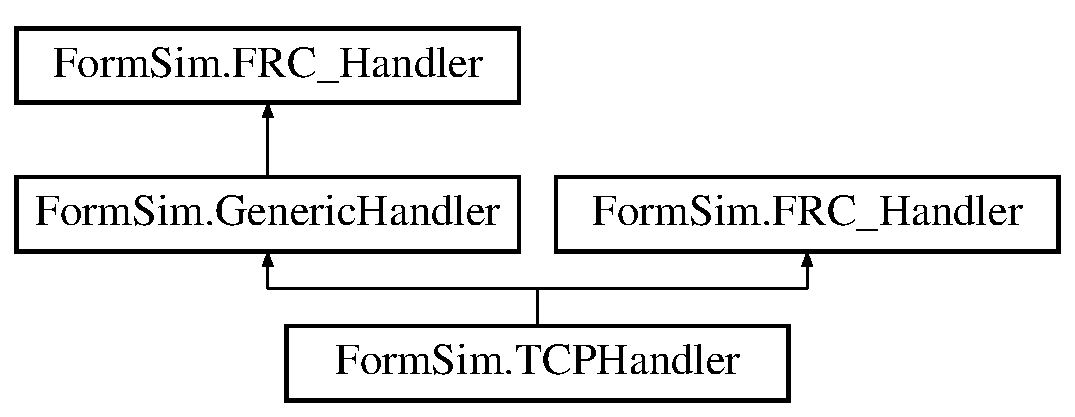
\includegraphics[height=3.000000cm]{class_form_sim_1_1_t_c_p_handler}
\end{center}
\end{figure}
\subsection*{Public Member Functions}
\begin{DoxyCompactItemize}
\item 
\mbox{\hyperlink{class_form_sim_1_1_t_c_p_handler_a26bcae2698f4403e85fbf24f3020eefb}{T\+C\+P\+Handler}} ()
\item 
\mbox{\hyperlink{class_form_sim_1_1_t_c_p_handler_a385ce1e4fcea1834b3f5b3ffae3f8b3c}{T\+C\+P\+Handler}} (string \mbox{\hyperlink{class_form_sim_1_1_generic_handler_a6699d8bfc9cd305baf30ab9413b21605}{Auth\+Token}}, string \mbox{\hyperlink{class_form_sim_1_1_generic_handler_ae1d2175b140f4c600d74bbab1e22714e}{Client\+G\+U\+ID}})
\item 
\mbox{\hyperlink{class_form_sim_1_1_t_c_p_handler_a40ec089c6d52e24b939e30127c9faeba}{T\+C\+P\+Handler}} (string \mbox{\hyperlink{class_form_sim_1_1_generic_handler_a6699d8bfc9cd305baf30ab9413b21605}{Auth\+Token}}, string \mbox{\hyperlink{class_form_sim_1_1_generic_handler_ae1d2175b140f4c600d74bbab1e22714e}{Client\+G\+U\+ID}}, string \mbox{\hyperlink{class_form_sim_1_1_generic_handler_a12b51dea082a4d40d86829802adf073b}{I\+P\+Address}}, string \mbox{\hyperlink{class_form_sim_1_1_generic_handler_ac6492bb3e4fbe8f66c97b00bd27020c1}{Port}})
\item 
override async Task$<$ bool $>$ \mbox{\hyperlink{class_form_sim_1_1_t_c_p_handler_a61075c8a24b97ae7c86d357d6ee5a49e}{perform\+Token\+Exchange}} ()
\begin{DoxyCompactList}\small\item\em Performs the token exchange with the client\+G\+U\+ID and Auth Token in exchange for an access token. N\+O\+TE\+: Both the client\+G\+U\+ID and the Auth\+Token must have been previously set or token exchange will fail. See \mbox{\hyperlink{interface_form_sim_1_1_f_r_c___handler_a3c77b2e99c98553928e463a9cbb5f7d4}{set\+Client\+G\+U\+I\+D(string)}} A\+ND See \mbox{\hyperlink{interface_form_sim_1_1_f_r_c___handler_a1314ea0937067435e3326818baa9d0c1}{set\+Auth\+Token(string)}} \end{DoxyCompactList}\item 
override async Task$<$ Dictionary$<$ string, string $>$ $>$ \mbox{\hyperlink{class_form_sim_1_1_t_c_p_handler_a810309bc6e943b6ff12ebed8401613f0}{send\+Raw}} (string raw\+Data)
\begin{DoxyCompactList}\small\item\em Sends a raw request to Shift4 for processing. This is mainly used as a debugging tool, to figure out if there are issues with the request, that can be deciphered ahead of hitting the Shift4 processing engine on the back side. This likely should be run in debug mode when full source is available as common errors that get thrown are not very descriptive. As time permits the error catching should be improved to hopefully throw more useful information about the actual error. \end{DoxyCompactList}\end{DoxyCompactItemize}
\subsection*{Protected Member Functions}
\begin{DoxyCompactItemize}
\item 
override async Task$<$ Dictionary$<$ string, string $>$ $>$ \mbox{\hyperlink{class_form_sim_1_1_t_c_p_handler_a7762d051722dd2ac8bee1c26043760f3}{perform\+Transaction}} (Dictionary$<$ string, string $>$ parameters)
\begin{DoxyCompactList}\small\item\em This method needs to be Overridden by a subclass. Method exists here only to allow complete compilation. \end{DoxyCompactList}\end{DoxyCompactItemize}
\subsection*{Private Member Functions}
\begin{DoxyCompactItemize}
\item 
Dictionary$<$ string, string $>$ \mbox{\hyperlink{class_form_sim_1_1_t_c_p_handler_a3c510f254bcd72de16d7824b89202878}{void\+Transaction}} (Dictionary$<$ string, string $>$ req, Dictionary$<$ string, string $>$ res)
\item 
string \mbox{\hyperlink{class_form_sim_1_1_t_c_p_handler_a5de578eeab047053441c0f5065e7258d}{build\+Transaction}} (Dictionary$<$ string, string $>$ parameters)
\item 
string \mbox{\hyperlink{class_form_sim_1_1_t_c_p_handler_a559496e83281e6dbfbc2010545465495}{build\+Transaction\+Header\+Data\+Block}} (string Function\+Request\+Code, string Requestor\+Reference, string Error\+Indicator, string Primary\+Error\+Code, string Secondary\+Error\+Code, string Merchant\+ID, string Tran\+ID, string Invoice, string Card\+Number)
\item 
string \mbox{\hyperlink{class_form_sim_1_1_t_c_p_handler_a87f8f6969a00e3c1f1f9510c3317c722}{build\+Vendor\+Block}} (string Vendor\+Description)
\item 
string \mbox{\hyperlink{class_form_sim_1_1_t_c_p_handler_a2790fa048c3f474f8690c7097310dd87}{build\+Standard\+Transaction\+Data\+Block}} (string Card\+Type, string Card\+Entry\+Mode, string Card\+Present, string Expiration\+Date, string Clerk, string Date, string Time, string Sale\+Flag, string Primary\+Amount, string Secondary\+Amount, string Response, string Authorization, string A\+V\+S\+Result, string A\+V\+S\+Street\+Verified, string A\+V\+S\+Zip\+Verified, string Valid\+A\+VS, string Track\+Information)
\item 
string \mbox{\hyperlink{class_form_sim_1_1_t_c_p_handler_a3fae46a36f1dfbc342a2af60be9805a7}{build\+A\+VS}} (string Customer\+Name, string Street\+Address, string Zip\+Code)
\item 
string \mbox{\hyperlink{class_form_sim_1_1_t_c_p_handler_afc287867c962d1863c17c82ce12d7907}{build\+Hotel\+Check\+Out}} (string Primary\+Charge\+Type, string Special\+Code, string Hotel\+Additional\+Charges, string Arrival\+Date, string Departure\+Date)
\item 
string \mbox{\hyperlink{class_form_sim_1_1_t_c_p_handler_a9f96d9f729c2dd000b31f7cafb5d19f8}{build\+Auto\+Return}} (string Rental\+Agreement, string Driver\+Name, string Late\+Adjustment, string Rental\+City, string Rental\+State, string Rental\+Zip\+Code, string Rental\+Date, string Rental\+Time, string Return\+City, string Return\+State, string Return\+Zip\+Code, string Return\+Date, string Return\+Time, string Auto\+Additional\+Charges, string No\+Show\+Indicator, string Return\+Country\+Code)
\item 
string \mbox{\hyperlink{class_form_sim_1_1_t_c_p_handler_aed895ee0544cd2dde70e21f36e6f4dea}{build\+Debit\+P\+I\+N\+Pad}} (string Pin\+Pad\+Type, string Pin\+Pad\+Block\+Format, string Pin\+Pad\+Key, string Pin\+Block)
\item 
string \mbox{\hyperlink{class_form_sim_1_1_t_c_p_handler_af6d62ad6f754a7cfd9fad3155e8c5f3d}{build\+Signature\+Capture}} (string Signature\+Device\+Type, string Signature\+Block\+Number, string Signature\+Total\+Blocks, string Signature\+Block)
\item 
string \mbox{\hyperlink{class_form_sim_1_1_t_c_p_handler_a4494caac6dd36e0e0594f65e005d026b}{build\+Level2\+Card\+Block}} (string Customer\+Reference, string Tax\+Indicator, string Tax\+Amount, string Destination\+Zip\+Code)
\item 
string \mbox{\hyperlink{class_form_sim_1_1_t_c_p_handler_afcfca846d1c87622f6cc3f5de84aba46}{build\+Purchasing\+Card\+Block}} (string Product\+Descriptor1, string Product\+Descriptor2, string Product\+Descriptor3, string Product\+Descriptor4)
\item 
string \mbox{\hyperlink{class_form_sim_1_1_t_c_p_handler_a380074a847d4b03c770e89785ff82862}{build\+Valid\+Check\+I\+D\+Types}} (string Valid\+I\+D\+Types)
\item 
string \mbox{\hyperlink{class_form_sim_1_1_t_c_p_handler_af66532d5978fe3b5e83e8ee48aa9cc8e}{build\+Check\+Approval}} (string I\+D\+Type\+Code, string I\+D\+Number, string Birthdate, string Check\+Amount, string Host\+Response, string Manual\+Check\+Number, string Raw\+Magnetic\+Data, string Check\+Type, string Reader\+Indicator, string Transit\+Routing\+Number, string Checking\+Account\+Number)
\item 
string \mbox{\hyperlink{class_form_sim_1_1_t_c_p_handler_a30576763872fd47bd1db76adffeaac2e}{build\+D\+BA}} (string D\+BA, string D\+B\+A\+Address\+Line1, string D\+B\+A\+Address\+Line2, string D\+B\+A\+City, string D\+B\+A\+State, string D\+B\+A\+Zip\+Code, string \mbox{\hyperlink{class_form_sim_1_1_generic_handler_a8b7d568966660d7d3700eac963caa504}{Merchant\+Type}}, string Card\+Abbreviations, string Serial\+Number, string Revision, string D\+B\+A\+Phone, string Business\+Day\+Ending\+Time)
\item 
string \mbox{\hyperlink{class_form_sim_1_1_t_c_p_handler_a0979d7d654863f637e6df1ad0af814c2}{build\+Hotel\+Check\+In}} (string Hotel\+Estimated\+Days)
\item 
string \mbox{\hyperlink{class_form_sim_1_1_t_c_p_handler_a6e587238891dd24c1b46b35c5fef08c4}{build\+Auto\+Rental}} (string Auto\+Estimated\+Days)
\item 
string \mbox{\hyperlink{class_form_sim_1_1_t_c_p_handler_a40eab47f3a9bffb4d3e4c35c060fabb9}{build\+Voice\+Authorization\+Center}} (string Voice\+Phone\+Number, string Voice\+Merchant\+Account)
\item 
string \mbox{\hyperlink{class_form_sim_1_1_t_c_p_handler_a06f7834b69ef0ec41b08ed992a6610a3}{build\+Extended\+Authorization}} (string Preauthorized\+Amount, string Preauthorized\+Tolerance, string Retrieval\+Reference, string Auth\+Source)
\item 
string \mbox{\hyperlink{class_form_sim_1_1_t_c_p_handler_acdb4cc9ece3eb8587fd41943cfbc7e71}{build\+Notes}} (string Notes)
\item 
string \mbox{\hyperlink{class_form_sim_1_1_t_c_p_handler_a19f3ec26051c3752e6fcd6813f7b3367}{build\+Terminal\+ID}} (string Terminal\+ID)
\item 
string \mbox{\hyperlink{class_form_sim_1_1_t_c_p_handler_afa361081bcfa04e9ba1e8cf2df615243}{build\+Card\+Security\+Code}} (string C\+V\+V2\+Indicator, string C\+V\+V2\+Code, string C\+V\+V2\+Result, string C\+V\+V2\+Valid)
\item 
string \mbox{\hyperlink{class_form_sim_1_1_t_c_p_handler_a3cd058e3a758ebd5231bd8f7f4bf4baa}{build\+A\+P\+I\+Options\+Data\+Block}} (string A\+P\+I\+Options)
\item 
string \mbox{\hyperlink{class_form_sim_1_1_t_c_p_handler_aaf84b1a98216bbe1e593574e31282e96}{build\+Its\+Your\+Card}} (string I\+Y\+C\+Card\+Type, string I\+Y\+C\+Discount, string I\+Y\+C\+Balance, string I\+Y\+C\+Available\+Balance, string I\+Y\+C\+Expiration, string I\+Y\+C\+Card\+Formatted)
\item 
string \mbox{\hyperlink{class_form_sim_1_1_t_c_p_handler_a64e2943ce2776de1fd819880fbf4a51e}{build\+Its\+Your\+Card\+Reason\+Text}} (string I\+Y\+C\+Reason\+Text)
\item 
string \mbox{\hyperlink{class_form_sim_1_1_t_c_p_handler_af5a1aa32467dd09d17c1a6a4c1d0b91a}{build\+Override\+Business\+Date}} (string Override\+Business\+Date)
\item 
string \mbox{\hyperlink{class_form_sim_1_1_t_c_p_handler_ad919a832ffdf9c14ba929af56eee5a59}{build\+Totals\+Report}} (string Report\+Start\+Date, string Report\+Start\+Time, string Report\+End\+Date, string Report\+End\+Time, string Report\+Clerk, string Report\+Card\+Type, string Report\+Terminal\+ID)
\item 
string \mbox{\hyperlink{class_form_sim_1_1_t_c_p_handler_a2815486693e9cd0075980b209cf9843c}{build\+Receipt\+Text}} (string Receipt\+Text\+Columns, string Receipt\+Text)
\item 
string \mbox{\hyperlink{class_form_sim_1_1_t_c_p_handler_ac8e49c8548bb66c3239b6f711afa3337}{build\+Unique\+ID}} (string Unique\+ID, string Token\+Serial\+Number)
\item 
string \mbox{\hyperlink{class_form_sim_1_1_t_c_p_handler_a05479dfb88131d0e857a6b882c60d21b}{build\+Line\+Items}} (string Line\+Item\+Count, string Line\+Item1, string Line\+Item2, string Line\+Item3, string Line\+Item4, string Line\+Item5, string Line\+Item6, string Line\+Item7, string Line\+Item8, string Line\+Item9, string Line\+Item10)
\item 
string \mbox{\hyperlink{class_form_sim_1_1_t_c_p_handler_ab3c968e347431409241d17aeebd02658}{build\+Line\+Item}} (string Line\+Item)
\item 
string \mbox{\hyperlink{class_form_sim_1_1_t_c_p_handler_a825fa707805dec081a03e08ff34deaef}{build\+Cashback\+And\+Surcharge\+Amounts}} (string Surcharge, string Cash\+Back)
\item 
string \mbox{\hyperlink{class_form_sim_1_1_t_c_p_handler_a74f16929ee87f2adcd72cb83041cb1c8}{build\+B\+I\+N\+Management}} (string Spin\+Prefix, string Spin\+Abb, string Spin\+Is\+Debit, string Spin\+Is\+D\+CC, string Spin\+Result)
\item 
string \mbox{\hyperlink{class_form_sim_1_1_t_c_p_handler_a378279fe5affb6172f80bed27f88d135}{build\+Enhanced\+Authorization}} (string Enhanced\+Data\+ID, string Enhanced\+Data\+Values)
\item 
string \mbox{\hyperlink{class_form_sim_1_1_t_c_p_handler_abdb585c67d61a7496cff8bb6d6375557}{build\+Inventory\+Information\+Approval\+System}} (string I\+I\+A\+S\+Type1, string I\+I\+A\+S\+Amount1, string I\+I\+A\+S\+Type2, string I\+I\+A\+S\+Amount2, string I\+I\+A\+S\+Type3, string I\+I\+A\+S\+Amount3, string I\+I\+A\+S\+Type4, string I\+I\+A\+S\+Amount4)
\item 
string \mbox{\hyperlink{class_form_sim_1_1_t_c_p_handler_a7d6134b876c094553e3b9cd4788711ee}{build\+Four\+Words}} (string Four\+Words)
\item 
string \mbox{\hyperlink{class_form_sim_1_1_t_c_p_handler_a059fa8efc59b79fcc0431b98692ef340}{build\+Card\+Level\+Results}} (string Card\+Level\+Results)
\item 
string \mbox{\hyperlink{class_form_sim_1_1_t_c_p_handler_a3400d87919fc5a21ecf0c824b5a638ce}{build\+Balance\+Return}} (string Balance\+Return\+Indicator, string Balance)
\item 
string \mbox{\hyperlink{class_form_sim_1_1_t_c_p_handler_ac81cff19c7ebc749ac9aca531b23791c}{build\+P2\+PE}} (string P2\+P\+E\+Block)
\item 
string \mbox{\hyperlink{class_form_sim_1_1_t_c_p_handler_a8da4a9dcb24a7ccefd0dde4522ed38e1}{build\+Meta\+Token}} (string Meta\+Token\+Type, string Meta\+Token\+Data)
\item 
string \mbox{\hyperlink{class_form_sim_1_1_t_c_p_handler_a37aa7ecd052c79a26fdac447ea6a72d4}{build\+Prompt\+Confirmation}} (string Prompt\+Confirm\+Result, string Prompt\+Confirm\+Question, string Prompt\+Confirm\+Value)
\item 
string \mbox{\hyperlink{class_form_sim_1_1_t_c_p_handler_a82c62d64444135157cb28449b445bd52}{build\+Photo}} (string Photo\+Type, string Photo\+Data)
\item 
string \mbox{\hyperlink{class_form_sim_1_1_t_c_p_handler_a48261051c49953461df8f0f5f6a8f0bc}{build\+Gift\+Card\+Extended\+Data}} (string Gift\+Card\+Extended\+Data\+Values)
\item 
string \mbox{\hyperlink{class_form_sim_1_1_t_c_p_handler_a8151b0587c3e38221d36a7e1b104be99}{build\+Merchant\+Receipt\+Text}} (string Merchant\+Receipt\+Text)
\item 
string \mbox{\hyperlink{class_form_sim_1_1_t_c_p_handler_aaf2b9db4f07dc72731543e366ae57f11}{build\+Customer\+Receipt\+Text}} (string Customer\+Receipt\+Text)
\item 
string \mbox{\hyperlink{class_form_sim_1_1_t_c_p_handler_a7026c44fa7957b4a223982a9b5b51b6c}{build\+Access\+Token\+Data\+Block}} (string \mbox{\hyperlink{class_form_sim_1_1_generic_handler_ad47864be2c5790106a7538f640b2792f}{Access\+Token}})
\item 
string \mbox{\hyperlink{class_form_sim_1_1_t_c_p_handler_aa04c2b705de9418eb13e35e01e1b784b}{build\+Token\+Exchange\+Data\+Block}} ()
\item 
string \mbox{\hyperlink{class_form_sim_1_1_t_c_p_handler_a7800a9d1eff8e2f38f22a8e4aebfed72}{build\+Cloud\+Parameters}} (string Device\+Service, string Device\+Guid)
\item 
string \mbox{\hyperlink{class_form_sim_1_1_t_c_p_handler_aae852cd3817353f951a7473471a1b9de}{build\+Cloud\+Extended\+Parameters}} (string Device\+Extensions)
\item 
string \mbox{\hyperlink{class_form_sim_1_1_t_c_p_handler_ad2df13eccffc001256e4a0265ef274c6}{build\+Process\+Forms}} (string Form\+Name, string Form\+Response, string Key\+Value1, string Key\+Value2, string Key\+Value3, string Key\+Value4, string Key\+Value5, string Key\+Value6, string Key\+Value7, string Key\+Value8, string Key\+Value9, string Key\+Value10)
\item 
string \mbox{\hyperlink{class_form_sim_1_1_t_c_p_handler_ab4c5c55715876db4c654f8a2abccceb6}{build\+Terms\+And\+Conditions}} (string Terms\+And\+Conditions\+Result, string Terms\+And\+Conditions)
\item 
string \mbox{\hyperlink{class_form_sim_1_1_t_c_p_handler_a633cebb97fe15074cbf3400eda7add31}{build\+Signature\+Suppressed}} (string Signature\+Suppressed)
\item 
string \mbox{\hyperlink{class_form_sim_1_1_t_c_p_handler_a1ccc91513b133900c48ca8b273d6a221}{build\+A\+V\+S\+\_\+\+C\+V\+V\+Prompt}} (string C\+V\+V2\+Prompt, string Street\+Number\+Prompt, string Postal\+Code\+Prompt)
\item 
string \mbox{\hyperlink{class_form_sim_1_1_t_c_p_handler_ab71d64e5e17fd1d66f5f803b0d5e1552}{build\+Input\+Prompt}} (string Device\+Input\+Index, string Device\+Input\+Response)
\item 
string \mbox{\hyperlink{class_form_sim_1_1_t_c_p_handler_a59e96abe11df9317a3c3b84fe5f4bd4b}{build\+Device\+Language}} (string Device\+Language)
\item 
string \mbox{\hyperlink{class_form_sim_1_1_t_c_p_handler_a402fdcb0d83b8508f15f996f26f9ef7e}{build\+Extended\+Error}} (string Short\+Error, string Long\+Error)
\item 
Dictionary$<$ string, string $>$ \mbox{\hyperlink{class_form_sim_1_1_t_c_p_handler_acd362681744f696310fde701c47309eb}{parse\+T\+C\+P\+Response}} (byte\mbox{[}$\,$\mbox{]} response)
\item 
void \mbox{\hyperlink{class_form_sim_1_1_t_c_p_handler_a25c22dcc9e98e6d182d62dd47a1cf7e0}{parse\+T\+C\+P\+Response\+Token}} (byte\mbox{[}$\,$\mbox{]} response)
\item 
Dictionary$<$ string, string $>$ \mbox{\hyperlink{class_form_sim_1_1_t_c_p_handler_ab274f99187a6bff02a17ec2c2e9c1d6a}{process\+Header\+Block}} (string block, Dictionary$<$ string, string $>$ dict)
\item 
Dictionary$<$ string, string $>$ \mbox{\hyperlink{class_form_sim_1_1_t_c_p_handler_abc4a88e1782473cc09b886e80e2a56dd}{process\+Vendor\+Block}} (char\mbox{[}$\,$\mbox{]} chars, Dictionary$<$ string, string $>$ dict)
\item 
Dictionary$<$ string, string $>$ \mbox{\hyperlink{class_form_sim_1_1_t_c_p_handler_ab1ebfa369393b79fda9bf02f2c1e4a94}{process\+Standard\+Transaction\+Block}} (char\mbox{[}$\,$\mbox{]} chars, Dictionary$<$ string, string $>$ dict)
\item 
Dictionary$<$ string, string $>$ \mbox{\hyperlink{class_form_sim_1_1_t_c_p_handler_ac58ef5265837b773924480e78f287737}{process\+A\+V\+S\+Block}} (char\mbox{[}$\,$\mbox{]} chars, Dictionary$<$ string, string $>$ dict)
\item 
Dictionary$<$ string, string $>$ \mbox{\hyperlink{class_form_sim_1_1_t_c_p_handler_a17c1a29be83e58752274a3ecb4d0c42d}{process\+Hotel\+Check\+Out}} (char\mbox{[}$\,$\mbox{]} chars, Dictionary$<$ string, string $>$ dict)
\item 
Dictionary$<$ string, string $>$ \mbox{\hyperlink{class_form_sim_1_1_t_c_p_handler_ab4fa317e40b02689b23b6decc5c4dd23}{process\+Auto\+Return}} (char\mbox{[}$\,$\mbox{]} chars, Dictionary$<$ string, string $>$ dict)
\item 
Dictionary$<$ string, string $>$ \mbox{\hyperlink{class_form_sim_1_1_t_c_p_handler_abee335961452418d460a7ae488ae3eb0}{process\+Debit\+P\+I\+N\+Pad}} (char\mbox{[}$\,$\mbox{]} chars, Dictionary$<$ string, string $>$ dict)
\item 
Dictionary$<$ string, string $>$ \mbox{\hyperlink{class_form_sim_1_1_t_c_p_handler_a26fb8948369426871f17ee0df07f9fae}{process\+Signature\+Capture}} (char\mbox{[}$\,$\mbox{]} chars, Dictionary$<$ string, string $>$ dict)
\item 
Dictionary$<$ string, string $>$ \mbox{\hyperlink{class_form_sim_1_1_t_c_p_handler_a68b477773fadcaaea8be6b8da1bfb0a5}{process\+Level2\+Card\+Block}} (char\mbox{[}$\,$\mbox{]} chars, Dictionary$<$ string, string $>$ dict)
\item 
Dictionary$<$ string, string $>$ \mbox{\hyperlink{class_form_sim_1_1_t_c_p_handler_afe54793d0d46b51163edf79a9733d6dd}{process\+Purchasing\+Card\+Block}} (char\mbox{[}$\,$\mbox{]} chars, Dictionary$<$ string, string $>$ dict)
\item 
Dictionary$<$ string, string $>$ \mbox{\hyperlink{class_form_sim_1_1_t_c_p_handler_a8f376aac84832a975e0a9334e2c208c5}{process\+Valid\+Check\+I\+D\+Types}} (char\mbox{[}$\,$\mbox{]} chars, Dictionary$<$ string, string $>$ dict)
\item 
Dictionary$<$ string, string $>$ \mbox{\hyperlink{class_form_sim_1_1_t_c_p_handler_af873827846e56cca37deb08de148c725}{process\+Check\+Approval}} (char\mbox{[}$\,$\mbox{]} chars, Dictionary$<$ string, string $>$ dict)
\item 
Dictionary$<$ string, string $>$ \mbox{\hyperlink{class_form_sim_1_1_t_c_p_handler_ac7fbe43d4623f2e14fc97882986e77c9}{process\+D\+BA}} (char\mbox{[}$\,$\mbox{]} chars, Dictionary$<$ string, string $>$ dict)
\item 
Dictionary$<$ string, string $>$ \mbox{\hyperlink{class_form_sim_1_1_t_c_p_handler_a42197084105edea21d65254ed1fc8ce4}{process\+Hotel\+Check\+In}} (char\mbox{[}$\,$\mbox{]} chars, Dictionary$<$ string, string $>$ dict)
\item 
Dictionary$<$ string, string $>$ \mbox{\hyperlink{class_form_sim_1_1_t_c_p_handler_a88eb6a78093ee2835b964fbf66653e7e}{process\+Auto\+Rental}} (char\mbox{[}$\,$\mbox{]} chars, Dictionary$<$ string, string $>$ dict)
\item 
Dictionary$<$ string, string $>$ \mbox{\hyperlink{class_form_sim_1_1_t_c_p_handler_a2c44efe0f4fd809a32174812bd2b7149}{process\+Voice\+Authorization\+Center}} (char\mbox{[}$\,$\mbox{]} chars, Dictionary$<$ string, string $>$ dict)
\item 
Dictionary$<$ string, string $>$ \mbox{\hyperlink{class_form_sim_1_1_t_c_p_handler_aeac1ea5fad517dbb64eae4c3039ea46f}{process\+Extended\+Authorization\+Block}} (char\mbox{[}$\,$\mbox{]} chars, Dictionary$<$ string, string $>$ dict)
\item 
Dictionary$<$ string, string $>$ \mbox{\hyperlink{class_form_sim_1_1_t_c_p_handler_ad4d752f756499196f766dc999f789fdb}{process\+Notes}} (char\mbox{[}$\,$\mbox{]} chars, Dictionary$<$ string, string $>$ dict)
\item 
Dictionary$<$ string, string $>$ \mbox{\hyperlink{class_form_sim_1_1_t_c_p_handler_a788a14473a58218eded09dcb8ab46fa3}{process\+Terminal\+ID}} (char\mbox{[}$\,$\mbox{]} chars, Dictionary$<$ string, string $>$ dict)
\item 
Dictionary$<$ string, string $>$ \mbox{\hyperlink{class_form_sim_1_1_t_c_p_handler_ab96b11e34b8e826ec6aa4644d413f85c}{process\+Card\+Security\+Code}} (char\mbox{[}$\,$\mbox{]} chars, Dictionary$<$ string, string $>$ dict)
\item 
Dictionary$<$ string, string $>$ \mbox{\hyperlink{class_form_sim_1_1_t_c_p_handler_a404ed1a6ccc26078fa89887505807598}{process\+A\+P\+I\+Options\+Block}} (char\mbox{[}$\,$\mbox{]} chars, Dictionary$<$ string, string $>$ dict)
\item 
Dictionary$<$ string, string $>$ \mbox{\hyperlink{class_form_sim_1_1_t_c_p_handler_a1957ee07ce1575f2e34669bff666dca1}{process\+Its\+Your\+Card}} (char\mbox{[}$\,$\mbox{]} chars, Dictionary$<$ string, string $>$ dict)
\item 
Dictionary$<$ string, string $>$ \mbox{\hyperlink{class_form_sim_1_1_t_c_p_handler_a6e499f837cfcf4ab08c81a3e14284087}{process\+Its\+Your\+Card\+Reason\+Text}} (char\mbox{[}$\,$\mbox{]} chars, Dictionary$<$ string, string $>$ dict)
\item 
Dictionary$<$ string, string $>$ \mbox{\hyperlink{class_form_sim_1_1_t_c_p_handler_a7e41880df196b83e6ea06d2551c4e230}{process\+Override\+Business\+Date}} (char\mbox{[}$\,$\mbox{]} chars, Dictionary$<$ string, string $>$ dict)
\item 
Dictionary$<$ string, string $>$ \mbox{\hyperlink{class_form_sim_1_1_t_c_p_handler_a9375cfb16933acd6cb6fd986f1c3f6c7}{process\+Totals\+Report}} (char\mbox{[}$\,$\mbox{]} chars, Dictionary$<$ string, string $>$ dict)
\item 
Dictionary$<$ string, string $>$ \mbox{\hyperlink{class_form_sim_1_1_t_c_p_handler_ac00f88ba9b49858e4d87b9e67e29aa87}{process\+Receipt\+Text\+Block}} (char\mbox{[}$\,$\mbox{]} chars, Dictionary$<$ string, string $>$ dict)
\item 
Dictionary$<$ string, string $>$ \mbox{\hyperlink{class_form_sim_1_1_t_c_p_handler_ac1914cfaa1d821983139e6af9a0ab79c}{process\+Unique\+I\+D\+Block}} (char\mbox{[}$\,$\mbox{]} chars, Dictionary$<$ string, string $>$ dict)
\item 
Dictionary$<$ string, string $>$ \mbox{\hyperlink{class_form_sim_1_1_t_c_p_handler_af20e4c201d008d4551c454e2e3203622}{process\+Line\+Items}} (char\mbox{[}$\,$\mbox{]} chars, Dictionary$<$ string, string $>$ dict)
\item 
Dictionary$<$ string, string $>$ \mbox{\hyperlink{class_form_sim_1_1_t_c_p_handler_a36fbcafba09f1511127e2ceaa0dac92b}{process\+Line\+Item}} (char\mbox{[}$\,$\mbox{]} chars, Dictionary$<$ string, string $>$ dict)
\item 
Dictionary$<$ string, string $>$ \mbox{\hyperlink{class_form_sim_1_1_t_c_p_handler_a5e5d6e5d1e9995cd5f212bac4eb9168a}{process\+Cashback\+And\+Surcharge\+Amounts}} (char\mbox{[}$\,$\mbox{]} chars, Dictionary$<$ string, string $>$ dict)
\item 
Dictionary$<$ string, string $>$ \mbox{\hyperlink{class_form_sim_1_1_t_c_p_handler_a1c458e61e4781a61d1cfa43e9347b3c6}{process\+B\+I\+N\+Management}} (char\mbox{[}$\,$\mbox{]} chars, Dictionary$<$ string, string $>$ dict)
\item 
Dictionary$<$ string, string $>$ \mbox{\hyperlink{class_form_sim_1_1_t_c_p_handler_aab0d3c1c8fc713dee9f077cfd3e2689c}{process\+Enhanced\+Authorization\+Block}} (char\mbox{[}$\,$\mbox{]} chars, Dictionary$<$ string, string $>$ dict)
\item 
Dictionary$<$ string, string $>$ \mbox{\hyperlink{class_form_sim_1_1_t_c_p_handler_accf737ffcc4e0d879f98978d85b005ae}{process\+Inventory\+Information\+Approval\+System}} (char\mbox{[}$\,$\mbox{]} chars, Dictionary$<$ string, string $>$ dict)
\item 
Dictionary$<$ string, string $>$ \mbox{\hyperlink{class_form_sim_1_1_t_c_p_handler_a0f25a73a16e6cea8f4fb65eb41ef8373}{process\+Four\+Words}} (char\mbox{[}$\,$\mbox{]} chars, Dictionary$<$ string, string $>$ dict)
\item 
Dictionary$<$ string, string $>$ \mbox{\hyperlink{class_form_sim_1_1_t_c_p_handler_aeaf47eddef345096f9e4db2c7b43592a}{process\+Card\+Level\+Results}} (char\mbox{[}$\,$\mbox{]} chars, Dictionary$<$ string, string $>$ dict)
\item 
Dictionary$<$ string, string $>$ \mbox{\hyperlink{class_form_sim_1_1_t_c_p_handler_a8edc653678104381cd77c4ec14808610}{process\+Balance\+Return\+Block}} (char\mbox{[}$\,$\mbox{]} chars, Dictionary$<$ string, string $>$ dict)
\item 
Dictionary$<$ string, string $>$ \mbox{\hyperlink{class_form_sim_1_1_t_c_p_handler_a1d7100333fad3bd76dd5abbff5b3cb9b}{process\+P2\+PE}} (char\mbox{[}$\,$\mbox{]} chars, Dictionary$<$ string, string $>$ dict)
\item 
Dictionary$<$ string, string $>$ \mbox{\hyperlink{class_form_sim_1_1_t_c_p_handler_a5eb9fa666902e313d7bb9ce9b73cbe7a}{process\+Meta\+Token}} (char\mbox{[}$\,$\mbox{]} chars, Dictionary$<$ string, string $>$ dict)
\item 
Dictionary$<$ string, string $>$ \mbox{\hyperlink{class_form_sim_1_1_t_c_p_handler_a8514434e5adb697c056d93f73aa849df}{process\+Prompt\+Confirmation}} (char\mbox{[}$\,$\mbox{]} chars, Dictionary$<$ string, string $>$ dict)
\item 
Dictionary$<$ string, string $>$ \mbox{\hyperlink{class_form_sim_1_1_t_c_p_handler_a17a26019d7633bcf35bdfc3be4c6b913}{process\+Photo}} (char\mbox{[}$\,$\mbox{]} chars, Dictionary$<$ string, string $>$ dict)
\item 
Dictionary$<$ string, string $>$ \mbox{\hyperlink{class_form_sim_1_1_t_c_p_handler_a767ff9ebb96f4da75c07d687fd71c2e7}{process\+Gift\+Card\+Extended\+Data}} (char\mbox{[}$\,$\mbox{]} chars, Dictionary$<$ string, string $>$ dict)
\item 
Dictionary$<$ string, string $>$ \mbox{\hyperlink{class_form_sim_1_1_t_c_p_handler_a7b39975f803ae5028bdfb874c6a9bb9c}{process\+Merchant\+Receipt\+Text}} (char\mbox{[}$\,$\mbox{]} chars, Dictionary$<$ string, string $>$ dict)
\item 
Dictionary$<$ string, string $>$ \mbox{\hyperlink{class_form_sim_1_1_t_c_p_handler_a45bb968cfd37e158b642677568096813}{process\+Customer\+Receipt\+Text}} (char\mbox{[}$\,$\mbox{]} chars, Dictionary$<$ string, string $>$ dict)
\item 
Dictionary$<$ string, string $>$ \mbox{\hyperlink{class_form_sim_1_1_t_c_p_handler_aedf978802bf4fee2c7b7529935da5bf3}{process\+Access\+Token\+Data\+Block}} (char\mbox{[}$\,$\mbox{]} chars, Dictionary$<$ string, string $>$ dict)
\item 
Dictionary$<$ string, string $>$ \mbox{\hyperlink{class_form_sim_1_1_t_c_p_handler_a5702eb572a0e7005cbe2bca58e591217}{process\+Token\+Exchange}} (char\mbox{[}$\,$\mbox{]} chars, Dictionary$<$ string, string $>$ dict)
\item 
Dictionary$<$ string, string $>$ \mbox{\hyperlink{class_form_sim_1_1_t_c_p_handler_a254b2c9aa486ecb07a994c417b20ff97}{process\+Cloud\+Parameters}} (char\mbox{[}$\,$\mbox{]} chars, Dictionary$<$ string, string $>$ dict)
\item 
Dictionary$<$ string, string $>$ \mbox{\hyperlink{class_form_sim_1_1_t_c_p_handler_a2cf69e45fed60fcef0c84fa7c98457e0}{process\+Cloud\+Extended\+Parameters}} (char\mbox{[}$\,$\mbox{]} chars, Dictionary$<$ string, string $>$ dict)
\item 
Dictionary$<$ string, string $>$ \mbox{\hyperlink{class_form_sim_1_1_t_c_p_handler_a3c2ddf21f92119ce435af5c3fbdb13b6}{process\+Process\+Forms}} (char\mbox{[}$\,$\mbox{]} chars, Dictionary$<$ string, string $>$ dict)
\item 
Dictionary$<$ string, string $>$ \mbox{\hyperlink{class_form_sim_1_1_t_c_p_handler_a3bd58ccb4d3137a26b8bd14080649bd4}{process\+Terms\+And\+Conditions}} (char\mbox{[}$\,$\mbox{]} chars, Dictionary$<$ string, string $>$ dict)
\item 
Dictionary$<$ string, string $>$ \mbox{\hyperlink{class_form_sim_1_1_t_c_p_handler_abbdc5072d534ac620abb7d9a48ba30a2}{process\+Signature\+Suppressed}} (char\mbox{[}$\,$\mbox{]} chars, Dictionary$<$ string, string $>$ dict)
\item 
Dictionary$<$ string, string $>$ \mbox{\hyperlink{class_form_sim_1_1_t_c_p_handler_ae6509869559cd7fac4e13e861510cc4b}{process\+A\+V\+S\+\_\+\+C\+V\+V\+Prompt}} (char\mbox{[}$\,$\mbox{]} chars, Dictionary$<$ string, string $>$ dict)
\item 
Dictionary$<$ string, string $>$ \mbox{\hyperlink{class_form_sim_1_1_t_c_p_handler_af9f544ae7073b4365be05307e9eae86a}{process\+Input\+Prompt}} (char\mbox{[}$\,$\mbox{]} chars, Dictionary$<$ string, string $>$ dict)
\item 
Dictionary$<$ string, string $>$ \mbox{\hyperlink{class_form_sim_1_1_t_c_p_handler_a08ab2569308a7bd09e5db8cd6d408459}{process\+Device\+Language}} (char\mbox{[}$\,$\mbox{]} chars, Dictionary$<$ string, string $>$ dict)
\item 
Dictionary$<$ string, string $>$ \mbox{\hyperlink{class_form_sim_1_1_t_c_p_handler_aadbaeefbb8bb128261c7cbf85be9c91c}{process\+Extended\+Error}} (char\mbox{[}$\,$\mbox{]} chars, Dictionary$<$ string, string $>$ dict)
\item 
string \mbox{\hyperlink{class_form_sim_1_1_t_c_p_handler_aa16ee3c9f634b4e00b7b2a7ec409fc89}{normalize}} (string to\+Be\+Normalized, int size)
\item 
string \mbox{\hyperlink{class_form_sim_1_1_t_c_p_handler_af33b52643998f6cdee82af449b8722ab}{right\+Pad}} (string to\+Be\+Padded, int size)
\item 
string \mbox{\hyperlink{class_form_sim_1_1_t_c_p_handler_afbcdb8bce1f946ff4549ed57786e85f7}{left\+Pad}} (string to\+Be\+Padded, int size)
\item 
string \mbox{\hyperlink{class_form_sim_1_1_t_c_p_handler_aa93d25e590a9ece741e94707b1f5d483}{truncate}} (string to\+Be\+Truncated, int size)
\end{DoxyCompactItemize}
\subsection*{Private Attributes}
\begin{DoxyCompactItemize}
\item 
Tcp\+Client \mbox{\hyperlink{class_form_sim_1_1_t_c_p_handler_ac98da866f5ae6c0eb8d772d7869f3158}{client}}
\end{DoxyCompactItemize}
\subsection*{Additional Inherited Members}


\subsection{Detailed Description}
The \mbox{\hyperlink{class_form_sim_1_1_t_c_p_handler}{T\+C\+P\+Handler}} class is designed to handle F\+R\+Cs over the T\+C\+P/\+IP protocol. Since this protocol uses byte sreams careful consideration must be made to ensure that transmission blocks are built appropraitely, and that received blocks are parsed appropriately. This implementation handles both of those scenarios. See \mbox{\hyperlink{class_form_sim_1_1_generic_handler}{Generic\+Handler}} for the best implementation strategy of dealing with F\+R\+Cs in general. 



\subsection{Constructor \& Destructor Documentation}
\mbox{\Hypertarget{class_form_sim_1_1_t_c_p_handler_a26bcae2698f4403e85fbf24f3020eefb}\label{class_form_sim_1_1_t_c_p_handler_a26bcae2698f4403e85fbf24f3020eefb}} 
\index{Form\+Sim\+::\+T\+C\+P\+Handler@{Form\+Sim\+::\+T\+C\+P\+Handler}!T\+C\+P\+Handler@{T\+C\+P\+Handler}}
\index{T\+C\+P\+Handler@{T\+C\+P\+Handler}!Form\+Sim\+::\+T\+C\+P\+Handler@{Form\+Sim\+::\+T\+C\+P\+Handler}}
\subsubsection{\texorpdfstring{T\+C\+P\+Handler()}{TCPHandler()}\hspace{0.1cm}{\footnotesize\ttfamily [1/3]}}
{\footnotesize\ttfamily Form\+Sim.\+T\+C\+P\+Handler.\+T\+C\+P\+Handler (\begin{DoxyParamCaption}{ }\end{DoxyParamCaption})\hspace{0.3cm}{\ttfamily [inline]}}

\mbox{\Hypertarget{class_form_sim_1_1_t_c_p_handler_a385ce1e4fcea1834b3f5b3ffae3f8b3c}\label{class_form_sim_1_1_t_c_p_handler_a385ce1e4fcea1834b3f5b3ffae3f8b3c}} 
\index{Form\+Sim\+::\+T\+C\+P\+Handler@{Form\+Sim\+::\+T\+C\+P\+Handler}!T\+C\+P\+Handler@{T\+C\+P\+Handler}}
\index{T\+C\+P\+Handler@{T\+C\+P\+Handler}!Form\+Sim\+::\+T\+C\+P\+Handler@{Form\+Sim\+::\+T\+C\+P\+Handler}}
\subsubsection{\texorpdfstring{T\+C\+P\+Handler()}{TCPHandler()}\hspace{0.1cm}{\footnotesize\ttfamily [2/3]}}
{\footnotesize\ttfamily Form\+Sim.\+T\+C\+P\+Handler.\+T\+C\+P\+Handler (\begin{DoxyParamCaption}\item[{string}]{Auth\+Token,  }\item[{string}]{Client\+G\+U\+ID }\end{DoxyParamCaption})\hspace{0.3cm}{\ttfamily [inline]}}

\mbox{\Hypertarget{class_form_sim_1_1_t_c_p_handler_a40ec089c6d52e24b939e30127c9faeba}\label{class_form_sim_1_1_t_c_p_handler_a40ec089c6d52e24b939e30127c9faeba}} 
\index{Form\+Sim\+::\+T\+C\+P\+Handler@{Form\+Sim\+::\+T\+C\+P\+Handler}!T\+C\+P\+Handler@{T\+C\+P\+Handler}}
\index{T\+C\+P\+Handler@{T\+C\+P\+Handler}!Form\+Sim\+::\+T\+C\+P\+Handler@{Form\+Sim\+::\+T\+C\+P\+Handler}}
\subsubsection{\texorpdfstring{T\+C\+P\+Handler()}{TCPHandler()}\hspace{0.1cm}{\footnotesize\ttfamily [3/3]}}
{\footnotesize\ttfamily Form\+Sim.\+T\+C\+P\+Handler.\+T\+C\+P\+Handler (\begin{DoxyParamCaption}\item[{string}]{Auth\+Token,  }\item[{string}]{Client\+G\+U\+ID,  }\item[{string}]{I\+P\+Address,  }\item[{string}]{Port }\end{DoxyParamCaption})\hspace{0.3cm}{\ttfamily [inline]}}



\subsection{Member Function Documentation}
\mbox{\Hypertarget{class_form_sim_1_1_t_c_p_handler_a7026c44fa7957b4a223982a9b5b51b6c}\label{class_form_sim_1_1_t_c_p_handler_a7026c44fa7957b4a223982a9b5b51b6c}} 
\index{Form\+Sim\+::\+T\+C\+P\+Handler@{Form\+Sim\+::\+T\+C\+P\+Handler}!build\+Access\+Token\+Data\+Block@{build\+Access\+Token\+Data\+Block}}
\index{build\+Access\+Token\+Data\+Block@{build\+Access\+Token\+Data\+Block}!Form\+Sim\+::\+T\+C\+P\+Handler@{Form\+Sim\+::\+T\+C\+P\+Handler}}
\subsubsection{\texorpdfstring{build\+Access\+Token\+Data\+Block()}{buildAccessTokenDataBlock()}}
{\footnotesize\ttfamily string Form\+Sim.\+T\+C\+P\+Handler.\+build\+Access\+Token\+Data\+Block (\begin{DoxyParamCaption}\item[{string}]{Access\+Token }\end{DoxyParamCaption})\hspace{0.3cm}{\ttfamily [inline]}, {\ttfamily [private]}}

\mbox{\Hypertarget{class_form_sim_1_1_t_c_p_handler_a3cd058e3a758ebd5231bd8f7f4bf4baa}\label{class_form_sim_1_1_t_c_p_handler_a3cd058e3a758ebd5231bd8f7f4bf4baa}} 
\index{Form\+Sim\+::\+T\+C\+P\+Handler@{Form\+Sim\+::\+T\+C\+P\+Handler}!build\+A\+P\+I\+Options\+Data\+Block@{build\+A\+P\+I\+Options\+Data\+Block}}
\index{build\+A\+P\+I\+Options\+Data\+Block@{build\+A\+P\+I\+Options\+Data\+Block}!Form\+Sim\+::\+T\+C\+P\+Handler@{Form\+Sim\+::\+T\+C\+P\+Handler}}
\subsubsection{\texorpdfstring{build\+A\+P\+I\+Options\+Data\+Block()}{buildAPIOptionsDataBlock()}}
{\footnotesize\ttfamily string Form\+Sim.\+T\+C\+P\+Handler.\+build\+A\+P\+I\+Options\+Data\+Block (\begin{DoxyParamCaption}\item[{string}]{A\+P\+I\+Options }\end{DoxyParamCaption})\hspace{0.3cm}{\ttfamily [inline]}, {\ttfamily [private]}}

\mbox{\Hypertarget{class_form_sim_1_1_t_c_p_handler_a6e587238891dd24c1b46b35c5fef08c4}\label{class_form_sim_1_1_t_c_p_handler_a6e587238891dd24c1b46b35c5fef08c4}} 
\index{Form\+Sim\+::\+T\+C\+P\+Handler@{Form\+Sim\+::\+T\+C\+P\+Handler}!build\+Auto\+Rental@{build\+Auto\+Rental}}
\index{build\+Auto\+Rental@{build\+Auto\+Rental}!Form\+Sim\+::\+T\+C\+P\+Handler@{Form\+Sim\+::\+T\+C\+P\+Handler}}
\subsubsection{\texorpdfstring{build\+Auto\+Rental()}{buildAutoRental()}}
{\footnotesize\ttfamily string Form\+Sim.\+T\+C\+P\+Handler.\+build\+Auto\+Rental (\begin{DoxyParamCaption}\item[{string}]{Auto\+Estimated\+Days }\end{DoxyParamCaption})\hspace{0.3cm}{\ttfamily [inline]}, {\ttfamily [private]}}

\mbox{\Hypertarget{class_form_sim_1_1_t_c_p_handler_a9f96d9f729c2dd000b31f7cafb5d19f8}\label{class_form_sim_1_1_t_c_p_handler_a9f96d9f729c2dd000b31f7cafb5d19f8}} 
\index{Form\+Sim\+::\+T\+C\+P\+Handler@{Form\+Sim\+::\+T\+C\+P\+Handler}!build\+Auto\+Return@{build\+Auto\+Return}}
\index{build\+Auto\+Return@{build\+Auto\+Return}!Form\+Sim\+::\+T\+C\+P\+Handler@{Form\+Sim\+::\+T\+C\+P\+Handler}}
\subsubsection{\texorpdfstring{build\+Auto\+Return()}{buildAutoReturn()}}
{\footnotesize\ttfamily string Form\+Sim.\+T\+C\+P\+Handler.\+build\+Auto\+Return (\begin{DoxyParamCaption}\item[{string}]{Rental\+Agreement,  }\item[{string}]{Driver\+Name,  }\item[{string}]{Late\+Adjustment,  }\item[{string}]{Rental\+City,  }\item[{string}]{Rental\+State,  }\item[{string}]{Rental\+Zip\+Code,  }\item[{string}]{Rental\+Date,  }\item[{string}]{Rental\+Time,  }\item[{string}]{Return\+City,  }\item[{string}]{Return\+State,  }\item[{string}]{Return\+Zip\+Code,  }\item[{string}]{Return\+Date,  }\item[{string}]{Return\+Time,  }\item[{string}]{Auto\+Additional\+Charges,  }\item[{string}]{No\+Show\+Indicator,  }\item[{string}]{Return\+Country\+Code }\end{DoxyParamCaption})\hspace{0.3cm}{\ttfamily [inline]}, {\ttfamily [private]}}

\mbox{\Hypertarget{class_form_sim_1_1_t_c_p_handler_a3fae46a36f1dfbc342a2af60be9805a7}\label{class_form_sim_1_1_t_c_p_handler_a3fae46a36f1dfbc342a2af60be9805a7}} 
\index{Form\+Sim\+::\+T\+C\+P\+Handler@{Form\+Sim\+::\+T\+C\+P\+Handler}!build\+A\+VS@{build\+A\+VS}}
\index{build\+A\+VS@{build\+A\+VS}!Form\+Sim\+::\+T\+C\+P\+Handler@{Form\+Sim\+::\+T\+C\+P\+Handler}}
\subsubsection{\texorpdfstring{build\+A\+V\+S()}{buildAVS()}}
{\footnotesize\ttfamily string Form\+Sim.\+T\+C\+P\+Handler.\+build\+A\+VS (\begin{DoxyParamCaption}\item[{string}]{Customer\+Name,  }\item[{string}]{Street\+Address,  }\item[{string}]{Zip\+Code }\end{DoxyParamCaption})\hspace{0.3cm}{\ttfamily [inline]}, {\ttfamily [private]}}

\mbox{\Hypertarget{class_form_sim_1_1_t_c_p_handler_a1ccc91513b133900c48ca8b273d6a221}\label{class_form_sim_1_1_t_c_p_handler_a1ccc91513b133900c48ca8b273d6a221}} 
\index{Form\+Sim\+::\+T\+C\+P\+Handler@{Form\+Sim\+::\+T\+C\+P\+Handler}!build\+A\+V\+S\+\_\+\+C\+V\+V\+Prompt@{build\+A\+V\+S\+\_\+\+C\+V\+V\+Prompt}}
\index{build\+A\+V\+S\+\_\+\+C\+V\+V\+Prompt@{build\+A\+V\+S\+\_\+\+C\+V\+V\+Prompt}!Form\+Sim\+::\+T\+C\+P\+Handler@{Form\+Sim\+::\+T\+C\+P\+Handler}}
\subsubsection{\texorpdfstring{build\+A\+V\+S\+\_\+\+C\+V\+V\+Prompt()}{buildAVS\_CVVPrompt()}}
{\footnotesize\ttfamily string Form\+Sim.\+T\+C\+P\+Handler.\+build\+A\+V\+S\+\_\+\+C\+V\+V\+Prompt (\begin{DoxyParamCaption}\item[{string}]{C\+V\+V2\+Prompt,  }\item[{string}]{Street\+Number\+Prompt,  }\item[{string}]{Postal\+Code\+Prompt }\end{DoxyParamCaption})\hspace{0.3cm}{\ttfamily [inline]}, {\ttfamily [private]}}

\mbox{\Hypertarget{class_form_sim_1_1_t_c_p_handler_a3400d87919fc5a21ecf0c824b5a638ce}\label{class_form_sim_1_1_t_c_p_handler_a3400d87919fc5a21ecf0c824b5a638ce}} 
\index{Form\+Sim\+::\+T\+C\+P\+Handler@{Form\+Sim\+::\+T\+C\+P\+Handler}!build\+Balance\+Return@{build\+Balance\+Return}}
\index{build\+Balance\+Return@{build\+Balance\+Return}!Form\+Sim\+::\+T\+C\+P\+Handler@{Form\+Sim\+::\+T\+C\+P\+Handler}}
\subsubsection{\texorpdfstring{build\+Balance\+Return()}{buildBalanceReturn()}}
{\footnotesize\ttfamily string Form\+Sim.\+T\+C\+P\+Handler.\+build\+Balance\+Return (\begin{DoxyParamCaption}\item[{string}]{Balance\+Return\+Indicator,  }\item[{string}]{Balance }\end{DoxyParamCaption})\hspace{0.3cm}{\ttfamily [inline]}, {\ttfamily [private]}}

\mbox{\Hypertarget{class_form_sim_1_1_t_c_p_handler_a74f16929ee87f2adcd72cb83041cb1c8}\label{class_form_sim_1_1_t_c_p_handler_a74f16929ee87f2adcd72cb83041cb1c8}} 
\index{Form\+Sim\+::\+T\+C\+P\+Handler@{Form\+Sim\+::\+T\+C\+P\+Handler}!build\+B\+I\+N\+Management@{build\+B\+I\+N\+Management}}
\index{build\+B\+I\+N\+Management@{build\+B\+I\+N\+Management}!Form\+Sim\+::\+T\+C\+P\+Handler@{Form\+Sim\+::\+T\+C\+P\+Handler}}
\subsubsection{\texorpdfstring{build\+B\+I\+N\+Management()}{buildBINManagement()}}
{\footnotesize\ttfamily string Form\+Sim.\+T\+C\+P\+Handler.\+build\+B\+I\+N\+Management (\begin{DoxyParamCaption}\item[{string}]{Spin\+Prefix,  }\item[{string}]{Spin\+Abb,  }\item[{string}]{Spin\+Is\+Debit,  }\item[{string}]{Spin\+Is\+D\+CC,  }\item[{string}]{Spin\+Result }\end{DoxyParamCaption})\hspace{0.3cm}{\ttfamily [inline]}, {\ttfamily [private]}}

\mbox{\Hypertarget{class_form_sim_1_1_t_c_p_handler_a059fa8efc59b79fcc0431b98692ef340}\label{class_form_sim_1_1_t_c_p_handler_a059fa8efc59b79fcc0431b98692ef340}} 
\index{Form\+Sim\+::\+T\+C\+P\+Handler@{Form\+Sim\+::\+T\+C\+P\+Handler}!build\+Card\+Level\+Results@{build\+Card\+Level\+Results}}
\index{build\+Card\+Level\+Results@{build\+Card\+Level\+Results}!Form\+Sim\+::\+T\+C\+P\+Handler@{Form\+Sim\+::\+T\+C\+P\+Handler}}
\subsubsection{\texorpdfstring{build\+Card\+Level\+Results()}{buildCardLevelResults()}}
{\footnotesize\ttfamily string Form\+Sim.\+T\+C\+P\+Handler.\+build\+Card\+Level\+Results (\begin{DoxyParamCaption}\item[{string}]{Card\+Level\+Results }\end{DoxyParamCaption})\hspace{0.3cm}{\ttfamily [inline]}, {\ttfamily [private]}}

\mbox{\Hypertarget{class_form_sim_1_1_t_c_p_handler_afa361081bcfa04e9ba1e8cf2df615243}\label{class_form_sim_1_1_t_c_p_handler_afa361081bcfa04e9ba1e8cf2df615243}} 
\index{Form\+Sim\+::\+T\+C\+P\+Handler@{Form\+Sim\+::\+T\+C\+P\+Handler}!build\+Card\+Security\+Code@{build\+Card\+Security\+Code}}
\index{build\+Card\+Security\+Code@{build\+Card\+Security\+Code}!Form\+Sim\+::\+T\+C\+P\+Handler@{Form\+Sim\+::\+T\+C\+P\+Handler}}
\subsubsection{\texorpdfstring{build\+Card\+Security\+Code()}{buildCardSecurityCode()}}
{\footnotesize\ttfamily string Form\+Sim.\+T\+C\+P\+Handler.\+build\+Card\+Security\+Code (\begin{DoxyParamCaption}\item[{string}]{C\+V\+V2\+Indicator,  }\item[{string}]{C\+V\+V2\+Code,  }\item[{string}]{C\+V\+V2\+Result,  }\item[{string}]{C\+V\+V2\+Valid }\end{DoxyParamCaption})\hspace{0.3cm}{\ttfamily [inline]}, {\ttfamily [private]}}

\mbox{\Hypertarget{class_form_sim_1_1_t_c_p_handler_a825fa707805dec081a03e08ff34deaef}\label{class_form_sim_1_1_t_c_p_handler_a825fa707805dec081a03e08ff34deaef}} 
\index{Form\+Sim\+::\+T\+C\+P\+Handler@{Form\+Sim\+::\+T\+C\+P\+Handler}!build\+Cashback\+And\+Surcharge\+Amounts@{build\+Cashback\+And\+Surcharge\+Amounts}}
\index{build\+Cashback\+And\+Surcharge\+Amounts@{build\+Cashback\+And\+Surcharge\+Amounts}!Form\+Sim\+::\+T\+C\+P\+Handler@{Form\+Sim\+::\+T\+C\+P\+Handler}}
\subsubsection{\texorpdfstring{build\+Cashback\+And\+Surcharge\+Amounts()}{buildCashbackAndSurchargeAmounts()}}
{\footnotesize\ttfamily string Form\+Sim.\+T\+C\+P\+Handler.\+build\+Cashback\+And\+Surcharge\+Amounts (\begin{DoxyParamCaption}\item[{string}]{Surcharge,  }\item[{string}]{Cash\+Back }\end{DoxyParamCaption})\hspace{0.3cm}{\ttfamily [inline]}, {\ttfamily [private]}}

\mbox{\Hypertarget{class_form_sim_1_1_t_c_p_handler_af66532d5978fe3b5e83e8ee48aa9cc8e}\label{class_form_sim_1_1_t_c_p_handler_af66532d5978fe3b5e83e8ee48aa9cc8e}} 
\index{Form\+Sim\+::\+T\+C\+P\+Handler@{Form\+Sim\+::\+T\+C\+P\+Handler}!build\+Check\+Approval@{build\+Check\+Approval}}
\index{build\+Check\+Approval@{build\+Check\+Approval}!Form\+Sim\+::\+T\+C\+P\+Handler@{Form\+Sim\+::\+T\+C\+P\+Handler}}
\subsubsection{\texorpdfstring{build\+Check\+Approval()}{buildCheckApproval()}}
{\footnotesize\ttfamily string Form\+Sim.\+T\+C\+P\+Handler.\+build\+Check\+Approval (\begin{DoxyParamCaption}\item[{string}]{I\+D\+Type\+Code,  }\item[{string}]{I\+D\+Number,  }\item[{string}]{Birthdate,  }\item[{string}]{Check\+Amount,  }\item[{string}]{Host\+Response,  }\item[{string}]{Manual\+Check\+Number,  }\item[{string}]{Raw\+Magnetic\+Data,  }\item[{string}]{Check\+Type,  }\item[{string}]{Reader\+Indicator,  }\item[{string}]{Transit\+Routing\+Number,  }\item[{string}]{Checking\+Account\+Number }\end{DoxyParamCaption})\hspace{0.3cm}{\ttfamily [inline]}, {\ttfamily [private]}}

\mbox{\Hypertarget{class_form_sim_1_1_t_c_p_handler_aae852cd3817353f951a7473471a1b9de}\label{class_form_sim_1_1_t_c_p_handler_aae852cd3817353f951a7473471a1b9de}} 
\index{Form\+Sim\+::\+T\+C\+P\+Handler@{Form\+Sim\+::\+T\+C\+P\+Handler}!build\+Cloud\+Extended\+Parameters@{build\+Cloud\+Extended\+Parameters}}
\index{build\+Cloud\+Extended\+Parameters@{build\+Cloud\+Extended\+Parameters}!Form\+Sim\+::\+T\+C\+P\+Handler@{Form\+Sim\+::\+T\+C\+P\+Handler}}
\subsubsection{\texorpdfstring{build\+Cloud\+Extended\+Parameters()}{buildCloudExtendedParameters()}}
{\footnotesize\ttfamily string Form\+Sim.\+T\+C\+P\+Handler.\+build\+Cloud\+Extended\+Parameters (\begin{DoxyParamCaption}\item[{string}]{Device\+Extensions }\end{DoxyParamCaption})\hspace{0.3cm}{\ttfamily [inline]}, {\ttfamily [private]}}

\mbox{\Hypertarget{class_form_sim_1_1_t_c_p_handler_a7800a9d1eff8e2f38f22a8e4aebfed72}\label{class_form_sim_1_1_t_c_p_handler_a7800a9d1eff8e2f38f22a8e4aebfed72}} 
\index{Form\+Sim\+::\+T\+C\+P\+Handler@{Form\+Sim\+::\+T\+C\+P\+Handler}!build\+Cloud\+Parameters@{build\+Cloud\+Parameters}}
\index{build\+Cloud\+Parameters@{build\+Cloud\+Parameters}!Form\+Sim\+::\+T\+C\+P\+Handler@{Form\+Sim\+::\+T\+C\+P\+Handler}}
\subsubsection{\texorpdfstring{build\+Cloud\+Parameters()}{buildCloudParameters()}}
{\footnotesize\ttfamily string Form\+Sim.\+T\+C\+P\+Handler.\+build\+Cloud\+Parameters (\begin{DoxyParamCaption}\item[{string}]{Device\+Service,  }\item[{string}]{Device\+Guid }\end{DoxyParamCaption})\hspace{0.3cm}{\ttfamily [inline]}, {\ttfamily [private]}}

\mbox{\Hypertarget{class_form_sim_1_1_t_c_p_handler_aaf2b9db4f07dc72731543e366ae57f11}\label{class_form_sim_1_1_t_c_p_handler_aaf2b9db4f07dc72731543e366ae57f11}} 
\index{Form\+Sim\+::\+T\+C\+P\+Handler@{Form\+Sim\+::\+T\+C\+P\+Handler}!build\+Customer\+Receipt\+Text@{build\+Customer\+Receipt\+Text}}
\index{build\+Customer\+Receipt\+Text@{build\+Customer\+Receipt\+Text}!Form\+Sim\+::\+T\+C\+P\+Handler@{Form\+Sim\+::\+T\+C\+P\+Handler}}
\subsubsection{\texorpdfstring{build\+Customer\+Receipt\+Text()}{buildCustomerReceiptText()}}
{\footnotesize\ttfamily string Form\+Sim.\+T\+C\+P\+Handler.\+build\+Customer\+Receipt\+Text (\begin{DoxyParamCaption}\item[{string}]{Customer\+Receipt\+Text }\end{DoxyParamCaption})\hspace{0.3cm}{\ttfamily [inline]}, {\ttfamily [private]}}

\mbox{\Hypertarget{class_form_sim_1_1_t_c_p_handler_a30576763872fd47bd1db76adffeaac2e}\label{class_form_sim_1_1_t_c_p_handler_a30576763872fd47bd1db76adffeaac2e}} 
\index{Form\+Sim\+::\+T\+C\+P\+Handler@{Form\+Sim\+::\+T\+C\+P\+Handler}!build\+D\+BA@{build\+D\+BA}}
\index{build\+D\+BA@{build\+D\+BA}!Form\+Sim\+::\+T\+C\+P\+Handler@{Form\+Sim\+::\+T\+C\+P\+Handler}}
\subsubsection{\texorpdfstring{build\+D\+B\+A()}{buildDBA()}}
{\footnotesize\ttfamily string Form\+Sim.\+T\+C\+P\+Handler.\+build\+D\+BA (\begin{DoxyParamCaption}\item[{string}]{D\+BA,  }\item[{string}]{D\+B\+A\+Address\+Line1,  }\item[{string}]{D\+B\+A\+Address\+Line2,  }\item[{string}]{D\+B\+A\+City,  }\item[{string}]{D\+B\+A\+State,  }\item[{string}]{D\+B\+A\+Zip\+Code,  }\item[{string}]{Merchant\+Type,  }\item[{string}]{Card\+Abbreviations,  }\item[{string}]{Serial\+Number,  }\item[{string}]{Revision,  }\item[{string}]{D\+B\+A\+Phone,  }\item[{string}]{Business\+Day\+Ending\+Time }\end{DoxyParamCaption})\hspace{0.3cm}{\ttfamily [inline]}, {\ttfamily [private]}}

\mbox{\Hypertarget{class_form_sim_1_1_t_c_p_handler_aed895ee0544cd2dde70e21f36e6f4dea}\label{class_form_sim_1_1_t_c_p_handler_aed895ee0544cd2dde70e21f36e6f4dea}} 
\index{Form\+Sim\+::\+T\+C\+P\+Handler@{Form\+Sim\+::\+T\+C\+P\+Handler}!build\+Debit\+P\+I\+N\+Pad@{build\+Debit\+P\+I\+N\+Pad}}
\index{build\+Debit\+P\+I\+N\+Pad@{build\+Debit\+P\+I\+N\+Pad}!Form\+Sim\+::\+T\+C\+P\+Handler@{Form\+Sim\+::\+T\+C\+P\+Handler}}
\subsubsection{\texorpdfstring{build\+Debit\+P\+I\+N\+Pad()}{buildDebitPINPad()}}
{\footnotesize\ttfamily string Form\+Sim.\+T\+C\+P\+Handler.\+build\+Debit\+P\+I\+N\+Pad (\begin{DoxyParamCaption}\item[{string}]{Pin\+Pad\+Type,  }\item[{string}]{Pin\+Pad\+Block\+Format,  }\item[{string}]{Pin\+Pad\+Key,  }\item[{string}]{Pin\+Block }\end{DoxyParamCaption})\hspace{0.3cm}{\ttfamily [inline]}, {\ttfamily [private]}}

\mbox{\Hypertarget{class_form_sim_1_1_t_c_p_handler_a59e96abe11df9317a3c3b84fe5f4bd4b}\label{class_form_sim_1_1_t_c_p_handler_a59e96abe11df9317a3c3b84fe5f4bd4b}} 
\index{Form\+Sim\+::\+T\+C\+P\+Handler@{Form\+Sim\+::\+T\+C\+P\+Handler}!build\+Device\+Language@{build\+Device\+Language}}
\index{build\+Device\+Language@{build\+Device\+Language}!Form\+Sim\+::\+T\+C\+P\+Handler@{Form\+Sim\+::\+T\+C\+P\+Handler}}
\subsubsection{\texorpdfstring{build\+Device\+Language()}{buildDeviceLanguage()}}
{\footnotesize\ttfamily string Form\+Sim.\+T\+C\+P\+Handler.\+build\+Device\+Language (\begin{DoxyParamCaption}\item[{string}]{Device\+Language }\end{DoxyParamCaption})\hspace{0.3cm}{\ttfamily [inline]}, {\ttfamily [private]}}

\mbox{\Hypertarget{class_form_sim_1_1_t_c_p_handler_a378279fe5affb6172f80bed27f88d135}\label{class_form_sim_1_1_t_c_p_handler_a378279fe5affb6172f80bed27f88d135}} 
\index{Form\+Sim\+::\+T\+C\+P\+Handler@{Form\+Sim\+::\+T\+C\+P\+Handler}!build\+Enhanced\+Authorization@{build\+Enhanced\+Authorization}}
\index{build\+Enhanced\+Authorization@{build\+Enhanced\+Authorization}!Form\+Sim\+::\+T\+C\+P\+Handler@{Form\+Sim\+::\+T\+C\+P\+Handler}}
\subsubsection{\texorpdfstring{build\+Enhanced\+Authorization()}{buildEnhancedAuthorization()}}
{\footnotesize\ttfamily string Form\+Sim.\+T\+C\+P\+Handler.\+build\+Enhanced\+Authorization (\begin{DoxyParamCaption}\item[{string}]{Enhanced\+Data\+ID,  }\item[{string}]{Enhanced\+Data\+Values }\end{DoxyParamCaption})\hspace{0.3cm}{\ttfamily [inline]}, {\ttfamily [private]}}

\mbox{\Hypertarget{class_form_sim_1_1_t_c_p_handler_a06f7834b69ef0ec41b08ed992a6610a3}\label{class_form_sim_1_1_t_c_p_handler_a06f7834b69ef0ec41b08ed992a6610a3}} 
\index{Form\+Sim\+::\+T\+C\+P\+Handler@{Form\+Sim\+::\+T\+C\+P\+Handler}!build\+Extended\+Authorization@{build\+Extended\+Authorization}}
\index{build\+Extended\+Authorization@{build\+Extended\+Authorization}!Form\+Sim\+::\+T\+C\+P\+Handler@{Form\+Sim\+::\+T\+C\+P\+Handler}}
\subsubsection{\texorpdfstring{build\+Extended\+Authorization()}{buildExtendedAuthorization()}}
{\footnotesize\ttfamily string Form\+Sim.\+T\+C\+P\+Handler.\+build\+Extended\+Authorization (\begin{DoxyParamCaption}\item[{string}]{Preauthorized\+Amount,  }\item[{string}]{Preauthorized\+Tolerance,  }\item[{string}]{Retrieval\+Reference,  }\item[{string}]{Auth\+Source }\end{DoxyParamCaption})\hspace{0.3cm}{\ttfamily [inline]}, {\ttfamily [private]}}

\mbox{\Hypertarget{class_form_sim_1_1_t_c_p_handler_a402fdcb0d83b8508f15f996f26f9ef7e}\label{class_form_sim_1_1_t_c_p_handler_a402fdcb0d83b8508f15f996f26f9ef7e}} 
\index{Form\+Sim\+::\+T\+C\+P\+Handler@{Form\+Sim\+::\+T\+C\+P\+Handler}!build\+Extended\+Error@{build\+Extended\+Error}}
\index{build\+Extended\+Error@{build\+Extended\+Error}!Form\+Sim\+::\+T\+C\+P\+Handler@{Form\+Sim\+::\+T\+C\+P\+Handler}}
\subsubsection{\texorpdfstring{build\+Extended\+Error()}{buildExtendedError()}}
{\footnotesize\ttfamily string Form\+Sim.\+T\+C\+P\+Handler.\+build\+Extended\+Error (\begin{DoxyParamCaption}\item[{string}]{Short\+Error,  }\item[{string}]{Long\+Error }\end{DoxyParamCaption})\hspace{0.3cm}{\ttfamily [inline]}, {\ttfamily [private]}}

\mbox{\Hypertarget{class_form_sim_1_1_t_c_p_handler_a7d6134b876c094553e3b9cd4788711ee}\label{class_form_sim_1_1_t_c_p_handler_a7d6134b876c094553e3b9cd4788711ee}} 
\index{Form\+Sim\+::\+T\+C\+P\+Handler@{Form\+Sim\+::\+T\+C\+P\+Handler}!build\+Four\+Words@{build\+Four\+Words}}
\index{build\+Four\+Words@{build\+Four\+Words}!Form\+Sim\+::\+T\+C\+P\+Handler@{Form\+Sim\+::\+T\+C\+P\+Handler}}
\subsubsection{\texorpdfstring{build\+Four\+Words()}{buildFourWords()}}
{\footnotesize\ttfamily string Form\+Sim.\+T\+C\+P\+Handler.\+build\+Four\+Words (\begin{DoxyParamCaption}\item[{string}]{Four\+Words }\end{DoxyParamCaption})\hspace{0.3cm}{\ttfamily [inline]}, {\ttfamily [private]}}

\mbox{\Hypertarget{class_form_sim_1_1_t_c_p_handler_a48261051c49953461df8f0f5f6a8f0bc}\label{class_form_sim_1_1_t_c_p_handler_a48261051c49953461df8f0f5f6a8f0bc}} 
\index{Form\+Sim\+::\+T\+C\+P\+Handler@{Form\+Sim\+::\+T\+C\+P\+Handler}!build\+Gift\+Card\+Extended\+Data@{build\+Gift\+Card\+Extended\+Data}}
\index{build\+Gift\+Card\+Extended\+Data@{build\+Gift\+Card\+Extended\+Data}!Form\+Sim\+::\+T\+C\+P\+Handler@{Form\+Sim\+::\+T\+C\+P\+Handler}}
\subsubsection{\texorpdfstring{build\+Gift\+Card\+Extended\+Data()}{buildGiftCardExtendedData()}}
{\footnotesize\ttfamily string Form\+Sim.\+T\+C\+P\+Handler.\+build\+Gift\+Card\+Extended\+Data (\begin{DoxyParamCaption}\item[{string}]{Gift\+Card\+Extended\+Data\+Values }\end{DoxyParamCaption})\hspace{0.3cm}{\ttfamily [inline]}, {\ttfamily [private]}}

\mbox{\Hypertarget{class_form_sim_1_1_t_c_p_handler_a0979d7d654863f637e6df1ad0af814c2}\label{class_form_sim_1_1_t_c_p_handler_a0979d7d654863f637e6df1ad0af814c2}} 
\index{Form\+Sim\+::\+T\+C\+P\+Handler@{Form\+Sim\+::\+T\+C\+P\+Handler}!build\+Hotel\+Check\+In@{build\+Hotel\+Check\+In}}
\index{build\+Hotel\+Check\+In@{build\+Hotel\+Check\+In}!Form\+Sim\+::\+T\+C\+P\+Handler@{Form\+Sim\+::\+T\+C\+P\+Handler}}
\subsubsection{\texorpdfstring{build\+Hotel\+Check\+In()}{buildHotelCheckIn()}}
{\footnotesize\ttfamily string Form\+Sim.\+T\+C\+P\+Handler.\+build\+Hotel\+Check\+In (\begin{DoxyParamCaption}\item[{string}]{Hotel\+Estimated\+Days }\end{DoxyParamCaption})\hspace{0.3cm}{\ttfamily [inline]}, {\ttfamily [private]}}

\mbox{\Hypertarget{class_form_sim_1_1_t_c_p_handler_afc287867c962d1863c17c82ce12d7907}\label{class_form_sim_1_1_t_c_p_handler_afc287867c962d1863c17c82ce12d7907}} 
\index{Form\+Sim\+::\+T\+C\+P\+Handler@{Form\+Sim\+::\+T\+C\+P\+Handler}!build\+Hotel\+Check\+Out@{build\+Hotel\+Check\+Out}}
\index{build\+Hotel\+Check\+Out@{build\+Hotel\+Check\+Out}!Form\+Sim\+::\+T\+C\+P\+Handler@{Form\+Sim\+::\+T\+C\+P\+Handler}}
\subsubsection{\texorpdfstring{build\+Hotel\+Check\+Out()}{buildHotelCheckOut()}}
{\footnotesize\ttfamily string Form\+Sim.\+T\+C\+P\+Handler.\+build\+Hotel\+Check\+Out (\begin{DoxyParamCaption}\item[{string}]{Primary\+Charge\+Type,  }\item[{string}]{Special\+Code,  }\item[{string}]{Hotel\+Additional\+Charges,  }\item[{string}]{Arrival\+Date,  }\item[{string}]{Departure\+Date }\end{DoxyParamCaption})\hspace{0.3cm}{\ttfamily [inline]}, {\ttfamily [private]}}

\mbox{\Hypertarget{class_form_sim_1_1_t_c_p_handler_ab71d64e5e17fd1d66f5f803b0d5e1552}\label{class_form_sim_1_1_t_c_p_handler_ab71d64e5e17fd1d66f5f803b0d5e1552}} 
\index{Form\+Sim\+::\+T\+C\+P\+Handler@{Form\+Sim\+::\+T\+C\+P\+Handler}!build\+Input\+Prompt@{build\+Input\+Prompt}}
\index{build\+Input\+Prompt@{build\+Input\+Prompt}!Form\+Sim\+::\+T\+C\+P\+Handler@{Form\+Sim\+::\+T\+C\+P\+Handler}}
\subsubsection{\texorpdfstring{build\+Input\+Prompt()}{buildInputPrompt()}}
{\footnotesize\ttfamily string Form\+Sim.\+T\+C\+P\+Handler.\+build\+Input\+Prompt (\begin{DoxyParamCaption}\item[{string}]{Device\+Input\+Index,  }\item[{string}]{Device\+Input\+Response }\end{DoxyParamCaption})\hspace{0.3cm}{\ttfamily [inline]}, {\ttfamily [private]}}

\mbox{\Hypertarget{class_form_sim_1_1_t_c_p_handler_abdb585c67d61a7496cff8bb6d6375557}\label{class_form_sim_1_1_t_c_p_handler_abdb585c67d61a7496cff8bb6d6375557}} 
\index{Form\+Sim\+::\+T\+C\+P\+Handler@{Form\+Sim\+::\+T\+C\+P\+Handler}!build\+Inventory\+Information\+Approval\+System@{build\+Inventory\+Information\+Approval\+System}}
\index{build\+Inventory\+Information\+Approval\+System@{build\+Inventory\+Information\+Approval\+System}!Form\+Sim\+::\+T\+C\+P\+Handler@{Form\+Sim\+::\+T\+C\+P\+Handler}}
\subsubsection{\texorpdfstring{build\+Inventory\+Information\+Approval\+System()}{buildInventoryInformationApprovalSystem()}}
{\footnotesize\ttfamily string Form\+Sim.\+T\+C\+P\+Handler.\+build\+Inventory\+Information\+Approval\+System (\begin{DoxyParamCaption}\item[{string}]{I\+I\+A\+S\+Type1,  }\item[{string}]{I\+I\+A\+S\+Amount1,  }\item[{string}]{I\+I\+A\+S\+Type2,  }\item[{string}]{I\+I\+A\+S\+Amount2,  }\item[{string}]{I\+I\+A\+S\+Type3,  }\item[{string}]{I\+I\+A\+S\+Amount3,  }\item[{string}]{I\+I\+A\+S\+Type4,  }\item[{string}]{I\+I\+A\+S\+Amount4 }\end{DoxyParamCaption})\hspace{0.3cm}{\ttfamily [inline]}, {\ttfamily [private]}}

\mbox{\Hypertarget{class_form_sim_1_1_t_c_p_handler_aaf84b1a98216bbe1e593574e31282e96}\label{class_form_sim_1_1_t_c_p_handler_aaf84b1a98216bbe1e593574e31282e96}} 
\index{Form\+Sim\+::\+T\+C\+P\+Handler@{Form\+Sim\+::\+T\+C\+P\+Handler}!build\+Its\+Your\+Card@{build\+Its\+Your\+Card}}
\index{build\+Its\+Your\+Card@{build\+Its\+Your\+Card}!Form\+Sim\+::\+T\+C\+P\+Handler@{Form\+Sim\+::\+T\+C\+P\+Handler}}
\subsubsection{\texorpdfstring{build\+Its\+Your\+Card()}{buildItsYourCard()}}
{\footnotesize\ttfamily string Form\+Sim.\+T\+C\+P\+Handler.\+build\+Its\+Your\+Card (\begin{DoxyParamCaption}\item[{string}]{I\+Y\+C\+Card\+Type,  }\item[{string}]{I\+Y\+C\+Discount,  }\item[{string}]{I\+Y\+C\+Balance,  }\item[{string}]{I\+Y\+C\+Available\+Balance,  }\item[{string}]{I\+Y\+C\+Expiration,  }\item[{string}]{I\+Y\+C\+Card\+Formatted }\end{DoxyParamCaption})\hspace{0.3cm}{\ttfamily [inline]}, {\ttfamily [private]}}

\mbox{\Hypertarget{class_form_sim_1_1_t_c_p_handler_a64e2943ce2776de1fd819880fbf4a51e}\label{class_form_sim_1_1_t_c_p_handler_a64e2943ce2776de1fd819880fbf4a51e}} 
\index{Form\+Sim\+::\+T\+C\+P\+Handler@{Form\+Sim\+::\+T\+C\+P\+Handler}!build\+Its\+Your\+Card\+Reason\+Text@{build\+Its\+Your\+Card\+Reason\+Text}}
\index{build\+Its\+Your\+Card\+Reason\+Text@{build\+Its\+Your\+Card\+Reason\+Text}!Form\+Sim\+::\+T\+C\+P\+Handler@{Form\+Sim\+::\+T\+C\+P\+Handler}}
\subsubsection{\texorpdfstring{build\+Its\+Your\+Card\+Reason\+Text()}{buildItsYourCardReasonText()}}
{\footnotesize\ttfamily string Form\+Sim.\+T\+C\+P\+Handler.\+build\+Its\+Your\+Card\+Reason\+Text (\begin{DoxyParamCaption}\item[{string}]{I\+Y\+C\+Reason\+Text }\end{DoxyParamCaption})\hspace{0.3cm}{\ttfamily [inline]}, {\ttfamily [private]}}

\mbox{\Hypertarget{class_form_sim_1_1_t_c_p_handler_a4494caac6dd36e0e0594f65e005d026b}\label{class_form_sim_1_1_t_c_p_handler_a4494caac6dd36e0e0594f65e005d026b}} 
\index{Form\+Sim\+::\+T\+C\+P\+Handler@{Form\+Sim\+::\+T\+C\+P\+Handler}!build\+Level2\+Card\+Block@{build\+Level2\+Card\+Block}}
\index{build\+Level2\+Card\+Block@{build\+Level2\+Card\+Block}!Form\+Sim\+::\+T\+C\+P\+Handler@{Form\+Sim\+::\+T\+C\+P\+Handler}}
\subsubsection{\texorpdfstring{build\+Level2\+Card\+Block()}{buildLevel2CardBlock()}}
{\footnotesize\ttfamily string Form\+Sim.\+T\+C\+P\+Handler.\+build\+Level2\+Card\+Block (\begin{DoxyParamCaption}\item[{string}]{Customer\+Reference,  }\item[{string}]{Tax\+Indicator,  }\item[{string}]{Tax\+Amount,  }\item[{string}]{Destination\+Zip\+Code }\end{DoxyParamCaption})\hspace{0.3cm}{\ttfamily [inline]}, {\ttfamily [private]}}

\mbox{\Hypertarget{class_form_sim_1_1_t_c_p_handler_ab3c968e347431409241d17aeebd02658}\label{class_form_sim_1_1_t_c_p_handler_ab3c968e347431409241d17aeebd02658}} 
\index{Form\+Sim\+::\+T\+C\+P\+Handler@{Form\+Sim\+::\+T\+C\+P\+Handler}!build\+Line\+Item@{build\+Line\+Item}}
\index{build\+Line\+Item@{build\+Line\+Item}!Form\+Sim\+::\+T\+C\+P\+Handler@{Form\+Sim\+::\+T\+C\+P\+Handler}}
\subsubsection{\texorpdfstring{build\+Line\+Item()}{buildLineItem()}}
{\footnotesize\ttfamily string Form\+Sim.\+T\+C\+P\+Handler.\+build\+Line\+Item (\begin{DoxyParamCaption}\item[{string}]{Line\+Item }\end{DoxyParamCaption})\hspace{0.3cm}{\ttfamily [inline]}, {\ttfamily [private]}}

\mbox{\Hypertarget{class_form_sim_1_1_t_c_p_handler_a05479dfb88131d0e857a6b882c60d21b}\label{class_form_sim_1_1_t_c_p_handler_a05479dfb88131d0e857a6b882c60d21b}} 
\index{Form\+Sim\+::\+T\+C\+P\+Handler@{Form\+Sim\+::\+T\+C\+P\+Handler}!build\+Line\+Items@{build\+Line\+Items}}
\index{build\+Line\+Items@{build\+Line\+Items}!Form\+Sim\+::\+T\+C\+P\+Handler@{Form\+Sim\+::\+T\+C\+P\+Handler}}
\subsubsection{\texorpdfstring{build\+Line\+Items()}{buildLineItems()}}
{\footnotesize\ttfamily string Form\+Sim.\+T\+C\+P\+Handler.\+build\+Line\+Items (\begin{DoxyParamCaption}\item[{string}]{Line\+Item\+Count,  }\item[{string}]{Line\+Item1,  }\item[{string}]{Line\+Item2,  }\item[{string}]{Line\+Item3,  }\item[{string}]{Line\+Item4,  }\item[{string}]{Line\+Item5,  }\item[{string}]{Line\+Item6,  }\item[{string}]{Line\+Item7,  }\item[{string}]{Line\+Item8,  }\item[{string}]{Line\+Item9,  }\item[{string}]{Line\+Item10 }\end{DoxyParamCaption})\hspace{0.3cm}{\ttfamily [inline]}, {\ttfamily [private]}}

\mbox{\Hypertarget{class_form_sim_1_1_t_c_p_handler_a8151b0587c3e38221d36a7e1b104be99}\label{class_form_sim_1_1_t_c_p_handler_a8151b0587c3e38221d36a7e1b104be99}} 
\index{Form\+Sim\+::\+T\+C\+P\+Handler@{Form\+Sim\+::\+T\+C\+P\+Handler}!build\+Merchant\+Receipt\+Text@{build\+Merchant\+Receipt\+Text}}
\index{build\+Merchant\+Receipt\+Text@{build\+Merchant\+Receipt\+Text}!Form\+Sim\+::\+T\+C\+P\+Handler@{Form\+Sim\+::\+T\+C\+P\+Handler}}
\subsubsection{\texorpdfstring{build\+Merchant\+Receipt\+Text()}{buildMerchantReceiptText()}}
{\footnotesize\ttfamily string Form\+Sim.\+T\+C\+P\+Handler.\+build\+Merchant\+Receipt\+Text (\begin{DoxyParamCaption}\item[{string}]{Merchant\+Receipt\+Text }\end{DoxyParamCaption})\hspace{0.3cm}{\ttfamily [inline]}, {\ttfamily [private]}}

\mbox{\Hypertarget{class_form_sim_1_1_t_c_p_handler_a8da4a9dcb24a7ccefd0dde4522ed38e1}\label{class_form_sim_1_1_t_c_p_handler_a8da4a9dcb24a7ccefd0dde4522ed38e1}} 
\index{Form\+Sim\+::\+T\+C\+P\+Handler@{Form\+Sim\+::\+T\+C\+P\+Handler}!build\+Meta\+Token@{build\+Meta\+Token}}
\index{build\+Meta\+Token@{build\+Meta\+Token}!Form\+Sim\+::\+T\+C\+P\+Handler@{Form\+Sim\+::\+T\+C\+P\+Handler}}
\subsubsection{\texorpdfstring{build\+Meta\+Token()}{buildMetaToken()}}
{\footnotesize\ttfamily string Form\+Sim.\+T\+C\+P\+Handler.\+build\+Meta\+Token (\begin{DoxyParamCaption}\item[{string}]{Meta\+Token\+Type,  }\item[{string}]{Meta\+Token\+Data }\end{DoxyParamCaption})\hspace{0.3cm}{\ttfamily [inline]}, {\ttfamily [private]}}

\mbox{\Hypertarget{class_form_sim_1_1_t_c_p_handler_acdb4cc9ece3eb8587fd41943cfbc7e71}\label{class_form_sim_1_1_t_c_p_handler_acdb4cc9ece3eb8587fd41943cfbc7e71}} 
\index{Form\+Sim\+::\+T\+C\+P\+Handler@{Form\+Sim\+::\+T\+C\+P\+Handler}!build\+Notes@{build\+Notes}}
\index{build\+Notes@{build\+Notes}!Form\+Sim\+::\+T\+C\+P\+Handler@{Form\+Sim\+::\+T\+C\+P\+Handler}}
\subsubsection{\texorpdfstring{build\+Notes()}{buildNotes()}}
{\footnotesize\ttfamily string Form\+Sim.\+T\+C\+P\+Handler.\+build\+Notes (\begin{DoxyParamCaption}\item[{string}]{Notes }\end{DoxyParamCaption})\hspace{0.3cm}{\ttfamily [inline]}, {\ttfamily [private]}}

\mbox{\Hypertarget{class_form_sim_1_1_t_c_p_handler_af5a1aa32467dd09d17c1a6a4c1d0b91a}\label{class_form_sim_1_1_t_c_p_handler_af5a1aa32467dd09d17c1a6a4c1d0b91a}} 
\index{Form\+Sim\+::\+T\+C\+P\+Handler@{Form\+Sim\+::\+T\+C\+P\+Handler}!build\+Override\+Business\+Date@{build\+Override\+Business\+Date}}
\index{build\+Override\+Business\+Date@{build\+Override\+Business\+Date}!Form\+Sim\+::\+T\+C\+P\+Handler@{Form\+Sim\+::\+T\+C\+P\+Handler}}
\subsubsection{\texorpdfstring{build\+Override\+Business\+Date()}{buildOverrideBusinessDate()}}
{\footnotesize\ttfamily string Form\+Sim.\+T\+C\+P\+Handler.\+build\+Override\+Business\+Date (\begin{DoxyParamCaption}\item[{string}]{Override\+Business\+Date }\end{DoxyParamCaption})\hspace{0.3cm}{\ttfamily [inline]}, {\ttfamily [private]}}

\mbox{\Hypertarget{class_form_sim_1_1_t_c_p_handler_ac81cff19c7ebc749ac9aca531b23791c}\label{class_form_sim_1_1_t_c_p_handler_ac81cff19c7ebc749ac9aca531b23791c}} 
\index{Form\+Sim\+::\+T\+C\+P\+Handler@{Form\+Sim\+::\+T\+C\+P\+Handler}!build\+P2\+PE@{build\+P2\+PE}}
\index{build\+P2\+PE@{build\+P2\+PE}!Form\+Sim\+::\+T\+C\+P\+Handler@{Form\+Sim\+::\+T\+C\+P\+Handler}}
\subsubsection{\texorpdfstring{build\+P2\+P\+E()}{buildP2PE()}}
{\footnotesize\ttfamily string Form\+Sim.\+T\+C\+P\+Handler.\+build\+P2\+PE (\begin{DoxyParamCaption}\item[{string}]{P2\+P\+E\+Block }\end{DoxyParamCaption})\hspace{0.3cm}{\ttfamily [inline]}, {\ttfamily [private]}}

\mbox{\Hypertarget{class_form_sim_1_1_t_c_p_handler_a82c62d64444135157cb28449b445bd52}\label{class_form_sim_1_1_t_c_p_handler_a82c62d64444135157cb28449b445bd52}} 
\index{Form\+Sim\+::\+T\+C\+P\+Handler@{Form\+Sim\+::\+T\+C\+P\+Handler}!build\+Photo@{build\+Photo}}
\index{build\+Photo@{build\+Photo}!Form\+Sim\+::\+T\+C\+P\+Handler@{Form\+Sim\+::\+T\+C\+P\+Handler}}
\subsubsection{\texorpdfstring{build\+Photo()}{buildPhoto()}}
{\footnotesize\ttfamily string Form\+Sim.\+T\+C\+P\+Handler.\+build\+Photo (\begin{DoxyParamCaption}\item[{string}]{Photo\+Type,  }\item[{string}]{Photo\+Data }\end{DoxyParamCaption})\hspace{0.3cm}{\ttfamily [inline]}, {\ttfamily [private]}}

\mbox{\Hypertarget{class_form_sim_1_1_t_c_p_handler_ad2df13eccffc001256e4a0265ef274c6}\label{class_form_sim_1_1_t_c_p_handler_ad2df13eccffc001256e4a0265ef274c6}} 
\index{Form\+Sim\+::\+T\+C\+P\+Handler@{Form\+Sim\+::\+T\+C\+P\+Handler}!build\+Process\+Forms@{build\+Process\+Forms}}
\index{build\+Process\+Forms@{build\+Process\+Forms}!Form\+Sim\+::\+T\+C\+P\+Handler@{Form\+Sim\+::\+T\+C\+P\+Handler}}
\subsubsection{\texorpdfstring{build\+Process\+Forms()}{buildProcessForms()}}
{\footnotesize\ttfamily string Form\+Sim.\+T\+C\+P\+Handler.\+build\+Process\+Forms (\begin{DoxyParamCaption}\item[{string}]{Form\+Name,  }\item[{string}]{Form\+Response,  }\item[{string}]{Key\+Value1,  }\item[{string}]{Key\+Value2,  }\item[{string}]{Key\+Value3,  }\item[{string}]{Key\+Value4,  }\item[{string}]{Key\+Value5,  }\item[{string}]{Key\+Value6,  }\item[{string}]{Key\+Value7,  }\item[{string}]{Key\+Value8,  }\item[{string}]{Key\+Value9,  }\item[{string}]{Key\+Value10 }\end{DoxyParamCaption})\hspace{0.3cm}{\ttfamily [inline]}, {\ttfamily [private]}}

\mbox{\Hypertarget{class_form_sim_1_1_t_c_p_handler_a37aa7ecd052c79a26fdac447ea6a72d4}\label{class_form_sim_1_1_t_c_p_handler_a37aa7ecd052c79a26fdac447ea6a72d4}} 
\index{Form\+Sim\+::\+T\+C\+P\+Handler@{Form\+Sim\+::\+T\+C\+P\+Handler}!build\+Prompt\+Confirmation@{build\+Prompt\+Confirmation}}
\index{build\+Prompt\+Confirmation@{build\+Prompt\+Confirmation}!Form\+Sim\+::\+T\+C\+P\+Handler@{Form\+Sim\+::\+T\+C\+P\+Handler}}
\subsubsection{\texorpdfstring{build\+Prompt\+Confirmation()}{buildPromptConfirmation()}}
{\footnotesize\ttfamily string Form\+Sim.\+T\+C\+P\+Handler.\+build\+Prompt\+Confirmation (\begin{DoxyParamCaption}\item[{string}]{Prompt\+Confirm\+Result,  }\item[{string}]{Prompt\+Confirm\+Question,  }\item[{string}]{Prompt\+Confirm\+Value }\end{DoxyParamCaption})\hspace{0.3cm}{\ttfamily [inline]}, {\ttfamily [private]}}

\mbox{\Hypertarget{class_form_sim_1_1_t_c_p_handler_afcfca846d1c87622f6cc3f5de84aba46}\label{class_form_sim_1_1_t_c_p_handler_afcfca846d1c87622f6cc3f5de84aba46}} 
\index{Form\+Sim\+::\+T\+C\+P\+Handler@{Form\+Sim\+::\+T\+C\+P\+Handler}!build\+Purchasing\+Card\+Block@{build\+Purchasing\+Card\+Block}}
\index{build\+Purchasing\+Card\+Block@{build\+Purchasing\+Card\+Block}!Form\+Sim\+::\+T\+C\+P\+Handler@{Form\+Sim\+::\+T\+C\+P\+Handler}}
\subsubsection{\texorpdfstring{build\+Purchasing\+Card\+Block()}{buildPurchasingCardBlock()}}
{\footnotesize\ttfamily string Form\+Sim.\+T\+C\+P\+Handler.\+build\+Purchasing\+Card\+Block (\begin{DoxyParamCaption}\item[{string}]{Product\+Descriptor1,  }\item[{string}]{Product\+Descriptor2,  }\item[{string}]{Product\+Descriptor3,  }\item[{string}]{Product\+Descriptor4 }\end{DoxyParamCaption})\hspace{0.3cm}{\ttfamily [inline]}, {\ttfamily [private]}}

\mbox{\Hypertarget{class_form_sim_1_1_t_c_p_handler_a2815486693e9cd0075980b209cf9843c}\label{class_form_sim_1_1_t_c_p_handler_a2815486693e9cd0075980b209cf9843c}} 
\index{Form\+Sim\+::\+T\+C\+P\+Handler@{Form\+Sim\+::\+T\+C\+P\+Handler}!build\+Receipt\+Text@{build\+Receipt\+Text}}
\index{build\+Receipt\+Text@{build\+Receipt\+Text}!Form\+Sim\+::\+T\+C\+P\+Handler@{Form\+Sim\+::\+T\+C\+P\+Handler}}
\subsubsection{\texorpdfstring{build\+Receipt\+Text()}{buildReceiptText()}}
{\footnotesize\ttfamily string Form\+Sim.\+T\+C\+P\+Handler.\+build\+Receipt\+Text (\begin{DoxyParamCaption}\item[{string}]{Receipt\+Text\+Columns,  }\item[{string}]{Receipt\+Text }\end{DoxyParamCaption})\hspace{0.3cm}{\ttfamily [inline]}, {\ttfamily [private]}}

\mbox{\Hypertarget{class_form_sim_1_1_t_c_p_handler_af6d62ad6f754a7cfd9fad3155e8c5f3d}\label{class_form_sim_1_1_t_c_p_handler_af6d62ad6f754a7cfd9fad3155e8c5f3d}} 
\index{Form\+Sim\+::\+T\+C\+P\+Handler@{Form\+Sim\+::\+T\+C\+P\+Handler}!build\+Signature\+Capture@{build\+Signature\+Capture}}
\index{build\+Signature\+Capture@{build\+Signature\+Capture}!Form\+Sim\+::\+T\+C\+P\+Handler@{Form\+Sim\+::\+T\+C\+P\+Handler}}
\subsubsection{\texorpdfstring{build\+Signature\+Capture()}{buildSignatureCapture()}}
{\footnotesize\ttfamily string Form\+Sim.\+T\+C\+P\+Handler.\+build\+Signature\+Capture (\begin{DoxyParamCaption}\item[{string}]{Signature\+Device\+Type,  }\item[{string}]{Signature\+Block\+Number,  }\item[{string}]{Signature\+Total\+Blocks,  }\item[{string}]{Signature\+Block }\end{DoxyParamCaption})\hspace{0.3cm}{\ttfamily [inline]}, {\ttfamily [private]}}

\mbox{\Hypertarget{class_form_sim_1_1_t_c_p_handler_a633cebb97fe15074cbf3400eda7add31}\label{class_form_sim_1_1_t_c_p_handler_a633cebb97fe15074cbf3400eda7add31}} 
\index{Form\+Sim\+::\+T\+C\+P\+Handler@{Form\+Sim\+::\+T\+C\+P\+Handler}!build\+Signature\+Suppressed@{build\+Signature\+Suppressed}}
\index{build\+Signature\+Suppressed@{build\+Signature\+Suppressed}!Form\+Sim\+::\+T\+C\+P\+Handler@{Form\+Sim\+::\+T\+C\+P\+Handler}}
\subsubsection{\texorpdfstring{build\+Signature\+Suppressed()}{buildSignatureSuppressed()}}
{\footnotesize\ttfamily string Form\+Sim.\+T\+C\+P\+Handler.\+build\+Signature\+Suppressed (\begin{DoxyParamCaption}\item[{string}]{Signature\+Suppressed }\end{DoxyParamCaption})\hspace{0.3cm}{\ttfamily [inline]}, {\ttfamily [private]}}

\mbox{\Hypertarget{class_form_sim_1_1_t_c_p_handler_a2790fa048c3f474f8690c7097310dd87}\label{class_form_sim_1_1_t_c_p_handler_a2790fa048c3f474f8690c7097310dd87}} 
\index{Form\+Sim\+::\+T\+C\+P\+Handler@{Form\+Sim\+::\+T\+C\+P\+Handler}!build\+Standard\+Transaction\+Data\+Block@{build\+Standard\+Transaction\+Data\+Block}}
\index{build\+Standard\+Transaction\+Data\+Block@{build\+Standard\+Transaction\+Data\+Block}!Form\+Sim\+::\+T\+C\+P\+Handler@{Form\+Sim\+::\+T\+C\+P\+Handler}}
\subsubsection{\texorpdfstring{build\+Standard\+Transaction\+Data\+Block()}{buildStandardTransactionDataBlock()}}
{\footnotesize\ttfamily string Form\+Sim.\+T\+C\+P\+Handler.\+build\+Standard\+Transaction\+Data\+Block (\begin{DoxyParamCaption}\item[{string}]{Card\+Type,  }\item[{string}]{Card\+Entry\+Mode,  }\item[{string}]{Card\+Present,  }\item[{string}]{Expiration\+Date,  }\item[{string}]{Clerk,  }\item[{string}]{Date,  }\item[{string}]{Time,  }\item[{string}]{Sale\+Flag,  }\item[{string}]{Primary\+Amount,  }\item[{string}]{Secondary\+Amount,  }\item[{string}]{Response,  }\item[{string}]{Authorization,  }\item[{string}]{A\+V\+S\+Result,  }\item[{string}]{A\+V\+S\+Street\+Verified,  }\item[{string}]{A\+V\+S\+Zip\+Verified,  }\item[{string}]{Valid\+A\+VS,  }\item[{string}]{Track\+Information }\end{DoxyParamCaption})\hspace{0.3cm}{\ttfamily [inline]}, {\ttfamily [private]}}

\mbox{\Hypertarget{class_form_sim_1_1_t_c_p_handler_a19f3ec26051c3752e6fcd6813f7b3367}\label{class_form_sim_1_1_t_c_p_handler_a19f3ec26051c3752e6fcd6813f7b3367}} 
\index{Form\+Sim\+::\+T\+C\+P\+Handler@{Form\+Sim\+::\+T\+C\+P\+Handler}!build\+Terminal\+ID@{build\+Terminal\+ID}}
\index{build\+Terminal\+ID@{build\+Terminal\+ID}!Form\+Sim\+::\+T\+C\+P\+Handler@{Form\+Sim\+::\+T\+C\+P\+Handler}}
\subsubsection{\texorpdfstring{build\+Terminal\+I\+D()}{buildTerminalID()}}
{\footnotesize\ttfamily string Form\+Sim.\+T\+C\+P\+Handler.\+build\+Terminal\+ID (\begin{DoxyParamCaption}\item[{string}]{Terminal\+ID }\end{DoxyParamCaption})\hspace{0.3cm}{\ttfamily [inline]}, {\ttfamily [private]}}

\mbox{\Hypertarget{class_form_sim_1_1_t_c_p_handler_ab4c5c55715876db4c654f8a2abccceb6}\label{class_form_sim_1_1_t_c_p_handler_ab4c5c55715876db4c654f8a2abccceb6}} 
\index{Form\+Sim\+::\+T\+C\+P\+Handler@{Form\+Sim\+::\+T\+C\+P\+Handler}!build\+Terms\+And\+Conditions@{build\+Terms\+And\+Conditions}}
\index{build\+Terms\+And\+Conditions@{build\+Terms\+And\+Conditions}!Form\+Sim\+::\+T\+C\+P\+Handler@{Form\+Sim\+::\+T\+C\+P\+Handler}}
\subsubsection{\texorpdfstring{build\+Terms\+And\+Conditions()}{buildTermsAndConditions()}}
{\footnotesize\ttfamily string Form\+Sim.\+T\+C\+P\+Handler.\+build\+Terms\+And\+Conditions (\begin{DoxyParamCaption}\item[{string}]{Terms\+And\+Conditions\+Result,  }\item[{string}]{Terms\+And\+Conditions }\end{DoxyParamCaption})\hspace{0.3cm}{\ttfamily [inline]}, {\ttfamily [private]}}

\mbox{\Hypertarget{class_form_sim_1_1_t_c_p_handler_aa04c2b705de9418eb13e35e01e1b784b}\label{class_form_sim_1_1_t_c_p_handler_aa04c2b705de9418eb13e35e01e1b784b}} 
\index{Form\+Sim\+::\+T\+C\+P\+Handler@{Form\+Sim\+::\+T\+C\+P\+Handler}!build\+Token\+Exchange\+Data\+Block@{build\+Token\+Exchange\+Data\+Block}}
\index{build\+Token\+Exchange\+Data\+Block@{build\+Token\+Exchange\+Data\+Block}!Form\+Sim\+::\+T\+C\+P\+Handler@{Form\+Sim\+::\+T\+C\+P\+Handler}}
\subsubsection{\texorpdfstring{build\+Token\+Exchange\+Data\+Block()}{buildTokenExchangeDataBlock()}}
{\footnotesize\ttfamily string Form\+Sim.\+T\+C\+P\+Handler.\+build\+Token\+Exchange\+Data\+Block (\begin{DoxyParamCaption}{ }\end{DoxyParamCaption})\hspace{0.3cm}{\ttfamily [inline]}, {\ttfamily [private]}}

\mbox{\Hypertarget{class_form_sim_1_1_t_c_p_handler_ad919a832ffdf9c14ba929af56eee5a59}\label{class_form_sim_1_1_t_c_p_handler_ad919a832ffdf9c14ba929af56eee5a59}} 
\index{Form\+Sim\+::\+T\+C\+P\+Handler@{Form\+Sim\+::\+T\+C\+P\+Handler}!build\+Totals\+Report@{build\+Totals\+Report}}
\index{build\+Totals\+Report@{build\+Totals\+Report}!Form\+Sim\+::\+T\+C\+P\+Handler@{Form\+Sim\+::\+T\+C\+P\+Handler}}
\subsubsection{\texorpdfstring{build\+Totals\+Report()}{buildTotalsReport()}}
{\footnotesize\ttfamily string Form\+Sim.\+T\+C\+P\+Handler.\+build\+Totals\+Report (\begin{DoxyParamCaption}\item[{string}]{Report\+Start\+Date,  }\item[{string}]{Report\+Start\+Time,  }\item[{string}]{Report\+End\+Date,  }\item[{string}]{Report\+End\+Time,  }\item[{string}]{Report\+Clerk,  }\item[{string}]{Report\+Card\+Type,  }\item[{string}]{Report\+Terminal\+ID }\end{DoxyParamCaption})\hspace{0.3cm}{\ttfamily [inline]}, {\ttfamily [private]}}

\mbox{\Hypertarget{class_form_sim_1_1_t_c_p_handler_a5de578eeab047053441c0f5065e7258d}\label{class_form_sim_1_1_t_c_p_handler_a5de578eeab047053441c0f5065e7258d}} 
\index{Form\+Sim\+::\+T\+C\+P\+Handler@{Form\+Sim\+::\+T\+C\+P\+Handler}!build\+Transaction@{build\+Transaction}}
\index{build\+Transaction@{build\+Transaction}!Form\+Sim\+::\+T\+C\+P\+Handler@{Form\+Sim\+::\+T\+C\+P\+Handler}}
\subsubsection{\texorpdfstring{build\+Transaction()}{buildTransaction()}}
{\footnotesize\ttfamily string Form\+Sim.\+T\+C\+P\+Handler.\+build\+Transaction (\begin{DoxyParamCaption}\item[{Dictionary$<$ string, string $>$}]{parameters }\end{DoxyParamCaption})\hspace{0.3cm}{\ttfamily [inline]}, {\ttfamily [private]}}

\mbox{\Hypertarget{class_form_sim_1_1_t_c_p_handler_a559496e83281e6dbfbc2010545465495}\label{class_form_sim_1_1_t_c_p_handler_a559496e83281e6dbfbc2010545465495}} 
\index{Form\+Sim\+::\+T\+C\+P\+Handler@{Form\+Sim\+::\+T\+C\+P\+Handler}!build\+Transaction\+Header\+Data\+Block@{build\+Transaction\+Header\+Data\+Block}}
\index{build\+Transaction\+Header\+Data\+Block@{build\+Transaction\+Header\+Data\+Block}!Form\+Sim\+::\+T\+C\+P\+Handler@{Form\+Sim\+::\+T\+C\+P\+Handler}}
\subsubsection{\texorpdfstring{build\+Transaction\+Header\+Data\+Block()}{buildTransactionHeaderDataBlock()}}
{\footnotesize\ttfamily string Form\+Sim.\+T\+C\+P\+Handler.\+build\+Transaction\+Header\+Data\+Block (\begin{DoxyParamCaption}\item[{string}]{Function\+Request\+Code,  }\item[{string}]{Requestor\+Reference,  }\item[{string}]{Error\+Indicator,  }\item[{string}]{Primary\+Error\+Code,  }\item[{string}]{Secondary\+Error\+Code,  }\item[{string}]{Merchant\+ID,  }\item[{string}]{Tran\+ID,  }\item[{string}]{Invoice,  }\item[{string}]{Card\+Number }\end{DoxyParamCaption})\hspace{0.3cm}{\ttfamily [inline]}, {\ttfamily [private]}}

\mbox{\Hypertarget{class_form_sim_1_1_t_c_p_handler_ac8e49c8548bb66c3239b6f711afa3337}\label{class_form_sim_1_1_t_c_p_handler_ac8e49c8548bb66c3239b6f711afa3337}} 
\index{Form\+Sim\+::\+T\+C\+P\+Handler@{Form\+Sim\+::\+T\+C\+P\+Handler}!build\+Unique\+ID@{build\+Unique\+ID}}
\index{build\+Unique\+ID@{build\+Unique\+ID}!Form\+Sim\+::\+T\+C\+P\+Handler@{Form\+Sim\+::\+T\+C\+P\+Handler}}
\subsubsection{\texorpdfstring{build\+Unique\+I\+D()}{buildUniqueID()}}
{\footnotesize\ttfamily string Form\+Sim.\+T\+C\+P\+Handler.\+build\+Unique\+ID (\begin{DoxyParamCaption}\item[{string}]{Unique\+ID,  }\item[{string}]{Token\+Serial\+Number }\end{DoxyParamCaption})\hspace{0.3cm}{\ttfamily [inline]}, {\ttfamily [private]}}

\mbox{\Hypertarget{class_form_sim_1_1_t_c_p_handler_a380074a847d4b03c770e89785ff82862}\label{class_form_sim_1_1_t_c_p_handler_a380074a847d4b03c770e89785ff82862}} 
\index{Form\+Sim\+::\+T\+C\+P\+Handler@{Form\+Sim\+::\+T\+C\+P\+Handler}!build\+Valid\+Check\+I\+D\+Types@{build\+Valid\+Check\+I\+D\+Types}}
\index{build\+Valid\+Check\+I\+D\+Types@{build\+Valid\+Check\+I\+D\+Types}!Form\+Sim\+::\+T\+C\+P\+Handler@{Form\+Sim\+::\+T\+C\+P\+Handler}}
\subsubsection{\texorpdfstring{build\+Valid\+Check\+I\+D\+Types()}{buildValidCheckIDTypes()}}
{\footnotesize\ttfamily string Form\+Sim.\+T\+C\+P\+Handler.\+build\+Valid\+Check\+I\+D\+Types (\begin{DoxyParamCaption}\item[{string}]{Valid\+I\+D\+Types }\end{DoxyParamCaption})\hspace{0.3cm}{\ttfamily [inline]}, {\ttfamily [private]}}

\mbox{\Hypertarget{class_form_sim_1_1_t_c_p_handler_a87f8f6969a00e3c1f1f9510c3317c722}\label{class_form_sim_1_1_t_c_p_handler_a87f8f6969a00e3c1f1f9510c3317c722}} 
\index{Form\+Sim\+::\+T\+C\+P\+Handler@{Form\+Sim\+::\+T\+C\+P\+Handler}!build\+Vendor\+Block@{build\+Vendor\+Block}}
\index{build\+Vendor\+Block@{build\+Vendor\+Block}!Form\+Sim\+::\+T\+C\+P\+Handler@{Form\+Sim\+::\+T\+C\+P\+Handler}}
\subsubsection{\texorpdfstring{build\+Vendor\+Block()}{buildVendorBlock()}}
{\footnotesize\ttfamily string Form\+Sim.\+T\+C\+P\+Handler.\+build\+Vendor\+Block (\begin{DoxyParamCaption}\item[{string}]{Vendor\+Description }\end{DoxyParamCaption})\hspace{0.3cm}{\ttfamily [inline]}, {\ttfamily [private]}}

\mbox{\Hypertarget{class_form_sim_1_1_t_c_p_handler_a40eab47f3a9bffb4d3e4c35c060fabb9}\label{class_form_sim_1_1_t_c_p_handler_a40eab47f3a9bffb4d3e4c35c060fabb9}} 
\index{Form\+Sim\+::\+T\+C\+P\+Handler@{Form\+Sim\+::\+T\+C\+P\+Handler}!build\+Voice\+Authorization\+Center@{build\+Voice\+Authorization\+Center}}
\index{build\+Voice\+Authorization\+Center@{build\+Voice\+Authorization\+Center}!Form\+Sim\+::\+T\+C\+P\+Handler@{Form\+Sim\+::\+T\+C\+P\+Handler}}
\subsubsection{\texorpdfstring{build\+Voice\+Authorization\+Center()}{buildVoiceAuthorizationCenter()}}
{\footnotesize\ttfamily string Form\+Sim.\+T\+C\+P\+Handler.\+build\+Voice\+Authorization\+Center (\begin{DoxyParamCaption}\item[{string}]{Voice\+Phone\+Number,  }\item[{string}]{Voice\+Merchant\+Account }\end{DoxyParamCaption})\hspace{0.3cm}{\ttfamily [inline]}, {\ttfamily [private]}}

\mbox{\Hypertarget{class_form_sim_1_1_t_c_p_handler_afbcdb8bce1f946ff4549ed57786e85f7}\label{class_form_sim_1_1_t_c_p_handler_afbcdb8bce1f946ff4549ed57786e85f7}} 
\index{Form\+Sim\+::\+T\+C\+P\+Handler@{Form\+Sim\+::\+T\+C\+P\+Handler}!left\+Pad@{left\+Pad}}
\index{left\+Pad@{left\+Pad}!Form\+Sim\+::\+T\+C\+P\+Handler@{Form\+Sim\+::\+T\+C\+P\+Handler}}
\subsubsection{\texorpdfstring{left\+Pad()}{leftPad()}}
{\footnotesize\ttfamily string Form\+Sim.\+T\+C\+P\+Handler.\+left\+Pad (\begin{DoxyParamCaption}\item[{string}]{to\+Be\+Padded,  }\item[{int}]{size }\end{DoxyParamCaption})\hspace{0.3cm}{\ttfamily [inline]}, {\ttfamily [private]}}

\mbox{\Hypertarget{class_form_sim_1_1_t_c_p_handler_aa16ee3c9f634b4e00b7b2a7ec409fc89}\label{class_form_sim_1_1_t_c_p_handler_aa16ee3c9f634b4e00b7b2a7ec409fc89}} 
\index{Form\+Sim\+::\+T\+C\+P\+Handler@{Form\+Sim\+::\+T\+C\+P\+Handler}!normalize@{normalize}}
\index{normalize@{normalize}!Form\+Sim\+::\+T\+C\+P\+Handler@{Form\+Sim\+::\+T\+C\+P\+Handler}}
\subsubsection{\texorpdfstring{normalize()}{normalize()}}
{\footnotesize\ttfamily string Form\+Sim.\+T\+C\+P\+Handler.\+normalize (\begin{DoxyParamCaption}\item[{string}]{to\+Be\+Normalized,  }\item[{int}]{size }\end{DoxyParamCaption})\hspace{0.3cm}{\ttfamily [inline]}, {\ttfamily [private]}}

\mbox{\Hypertarget{class_form_sim_1_1_t_c_p_handler_acd362681744f696310fde701c47309eb}\label{class_form_sim_1_1_t_c_p_handler_acd362681744f696310fde701c47309eb}} 
\index{Form\+Sim\+::\+T\+C\+P\+Handler@{Form\+Sim\+::\+T\+C\+P\+Handler}!parse\+T\+C\+P\+Response@{parse\+T\+C\+P\+Response}}
\index{parse\+T\+C\+P\+Response@{parse\+T\+C\+P\+Response}!Form\+Sim\+::\+T\+C\+P\+Handler@{Form\+Sim\+::\+T\+C\+P\+Handler}}
\subsubsection{\texorpdfstring{parse\+T\+C\+P\+Response()}{parseTCPResponse()}}
{\footnotesize\ttfamily Dictionary$<$string, string$>$ Form\+Sim.\+T\+C\+P\+Handler.\+parse\+T\+C\+P\+Response (\begin{DoxyParamCaption}\item[{byte \mbox{[}$\,$\mbox{]}}]{response }\end{DoxyParamCaption})\hspace{0.3cm}{\ttfamily [inline]}, {\ttfamily [private]}}

\mbox{\Hypertarget{class_form_sim_1_1_t_c_p_handler_a25c22dcc9e98e6d182d62dd47a1cf7e0}\label{class_form_sim_1_1_t_c_p_handler_a25c22dcc9e98e6d182d62dd47a1cf7e0}} 
\index{Form\+Sim\+::\+T\+C\+P\+Handler@{Form\+Sim\+::\+T\+C\+P\+Handler}!parse\+T\+C\+P\+Response\+Token@{parse\+T\+C\+P\+Response\+Token}}
\index{parse\+T\+C\+P\+Response\+Token@{parse\+T\+C\+P\+Response\+Token}!Form\+Sim\+::\+T\+C\+P\+Handler@{Form\+Sim\+::\+T\+C\+P\+Handler}}
\subsubsection{\texorpdfstring{parse\+T\+C\+P\+Response\+Token()}{parseTCPResponseToken()}}
{\footnotesize\ttfamily void Form\+Sim.\+T\+C\+P\+Handler.\+parse\+T\+C\+P\+Response\+Token (\begin{DoxyParamCaption}\item[{byte \mbox{[}$\,$\mbox{]}}]{response }\end{DoxyParamCaption})\hspace{0.3cm}{\ttfamily [inline]}, {\ttfamily [private]}}

\mbox{\Hypertarget{class_form_sim_1_1_t_c_p_handler_a61075c8a24b97ae7c86d357d6ee5a49e}\label{class_form_sim_1_1_t_c_p_handler_a61075c8a24b97ae7c86d357d6ee5a49e}} 
\index{Form\+Sim\+::\+T\+C\+P\+Handler@{Form\+Sim\+::\+T\+C\+P\+Handler}!perform\+Token\+Exchange@{perform\+Token\+Exchange}}
\index{perform\+Token\+Exchange@{perform\+Token\+Exchange}!Form\+Sim\+::\+T\+C\+P\+Handler@{Form\+Sim\+::\+T\+C\+P\+Handler}}
\subsubsection{\texorpdfstring{perform\+Token\+Exchange()}{performTokenExchange()}}
{\footnotesize\ttfamily override async Task$<$bool$>$ Form\+Sim.\+T\+C\+P\+Handler.\+perform\+Token\+Exchange (\begin{DoxyParamCaption}{ }\end{DoxyParamCaption})\hspace{0.3cm}{\ttfamily [inline]}}



Performs the token exchange with the client\+G\+U\+ID and Auth Token in exchange for an access token. N\+O\+TE\+: Both the client\+G\+U\+ID and the Auth\+Token must have been previously set or token exchange will fail. See \mbox{\hyperlink{interface_form_sim_1_1_f_r_c___handler_a3c77b2e99c98553928e463a9cbb5f7d4}{set\+Client\+G\+U\+I\+D(string)}} A\+ND See \mbox{\hyperlink{interface_form_sim_1_1_f_r_c___handler_a1314ea0937067435e3326818baa9d0c1}{set\+Auth\+Token(string)}} 

\begin{DoxyReturn}{Returns}
True if an Access token was received and set, false otherwise
\end{DoxyReturn}


Implements \mbox{\hyperlink{interface_form_sim_1_1_f_r_c___handler_a32c299d3cb3cdd6c444e76b3671af1b4}{Form\+Sim.\+F\+R\+C\+\_\+\+Handler}}.

\mbox{\Hypertarget{class_form_sim_1_1_t_c_p_handler_a7762d051722dd2ac8bee1c26043760f3}\label{class_form_sim_1_1_t_c_p_handler_a7762d051722dd2ac8bee1c26043760f3}} 
\index{Form\+Sim\+::\+T\+C\+P\+Handler@{Form\+Sim\+::\+T\+C\+P\+Handler}!perform\+Transaction@{perform\+Transaction}}
\index{perform\+Transaction@{perform\+Transaction}!Form\+Sim\+::\+T\+C\+P\+Handler@{Form\+Sim\+::\+T\+C\+P\+Handler}}
\subsubsection{\texorpdfstring{perform\+Transaction()}{performTransaction()}}
{\footnotesize\ttfamily override async Task$<$Dictionary$<$string, string$>$ $>$ Form\+Sim.\+T\+C\+P\+Handler.\+perform\+Transaction (\begin{DoxyParamCaption}\item[{Dictionary$<$ string, string $>$}]{parameters }\end{DoxyParamCaption})\hspace{0.3cm}{\ttfamily [inline]}, {\ttfamily [protected]}, {\ttfamily [virtual]}}



This method needs to be Overridden by a subclass. Method exists here only to allow complete compilation. 


\begin{DoxyExceptions}{Exceptions}
{\em Not\+Implemented\+Exception} & If not overridden.\\
\hline
\end{DoxyExceptions}

\begin{DoxyParams}{Parameters}
{\em parameters} & A dictionary of parameters sent from the front end. See \mbox{\hyperlink{interface_form_sim_1_1_f_r_c___handler_a2a2a8a776e774e5f8b5e2b7e623a26a6}{F\+R\+C\+\_\+\+Handler.\+start(\+Dictionary$<$string, string$>$)}} for a listing of the parameters in the Dictionary.\\
\hline
\end{DoxyParams}
\begin{DoxyReturn}{Returns}
A thread with the results of the F\+RC in a dictionary.
\end{DoxyReturn}


Reimplemented from \mbox{\hyperlink{class_form_sim_1_1_generic_handler_a824697e5c22a4f1cf8ce4e512b6954ad}{Form\+Sim.\+Generic\+Handler}}.

\mbox{\Hypertarget{class_form_sim_1_1_t_c_p_handler_aedf978802bf4fee2c7b7529935da5bf3}\label{class_form_sim_1_1_t_c_p_handler_aedf978802bf4fee2c7b7529935da5bf3}} 
\index{Form\+Sim\+::\+T\+C\+P\+Handler@{Form\+Sim\+::\+T\+C\+P\+Handler}!process\+Access\+Token\+Data\+Block@{process\+Access\+Token\+Data\+Block}}
\index{process\+Access\+Token\+Data\+Block@{process\+Access\+Token\+Data\+Block}!Form\+Sim\+::\+T\+C\+P\+Handler@{Form\+Sim\+::\+T\+C\+P\+Handler}}
\subsubsection{\texorpdfstring{process\+Access\+Token\+Data\+Block()}{processAccessTokenDataBlock()}}
{\footnotesize\ttfamily Dictionary$<$string, string$>$ Form\+Sim.\+T\+C\+P\+Handler.\+process\+Access\+Token\+Data\+Block (\begin{DoxyParamCaption}\item[{char \mbox{[}$\,$\mbox{]}}]{chars,  }\item[{Dictionary$<$ string, string $>$}]{dict }\end{DoxyParamCaption})\hspace{0.3cm}{\ttfamily [inline]}, {\ttfamily [private]}}

\mbox{\Hypertarget{class_form_sim_1_1_t_c_p_handler_a404ed1a6ccc26078fa89887505807598}\label{class_form_sim_1_1_t_c_p_handler_a404ed1a6ccc26078fa89887505807598}} 
\index{Form\+Sim\+::\+T\+C\+P\+Handler@{Form\+Sim\+::\+T\+C\+P\+Handler}!process\+A\+P\+I\+Options\+Block@{process\+A\+P\+I\+Options\+Block}}
\index{process\+A\+P\+I\+Options\+Block@{process\+A\+P\+I\+Options\+Block}!Form\+Sim\+::\+T\+C\+P\+Handler@{Form\+Sim\+::\+T\+C\+P\+Handler}}
\subsubsection{\texorpdfstring{process\+A\+P\+I\+Options\+Block()}{processAPIOptionsBlock()}}
{\footnotesize\ttfamily Dictionary$<$string, string$>$ Form\+Sim.\+T\+C\+P\+Handler.\+process\+A\+P\+I\+Options\+Block (\begin{DoxyParamCaption}\item[{char \mbox{[}$\,$\mbox{]}}]{chars,  }\item[{Dictionary$<$ string, string $>$}]{dict }\end{DoxyParamCaption})\hspace{0.3cm}{\ttfamily [inline]}, {\ttfamily [private]}}

\mbox{\Hypertarget{class_form_sim_1_1_t_c_p_handler_a88eb6a78093ee2835b964fbf66653e7e}\label{class_form_sim_1_1_t_c_p_handler_a88eb6a78093ee2835b964fbf66653e7e}} 
\index{Form\+Sim\+::\+T\+C\+P\+Handler@{Form\+Sim\+::\+T\+C\+P\+Handler}!process\+Auto\+Rental@{process\+Auto\+Rental}}
\index{process\+Auto\+Rental@{process\+Auto\+Rental}!Form\+Sim\+::\+T\+C\+P\+Handler@{Form\+Sim\+::\+T\+C\+P\+Handler}}
\subsubsection{\texorpdfstring{process\+Auto\+Rental()}{processAutoRental()}}
{\footnotesize\ttfamily Dictionary$<$string, string$>$ Form\+Sim.\+T\+C\+P\+Handler.\+process\+Auto\+Rental (\begin{DoxyParamCaption}\item[{char \mbox{[}$\,$\mbox{]}}]{chars,  }\item[{Dictionary$<$ string, string $>$}]{dict }\end{DoxyParamCaption})\hspace{0.3cm}{\ttfamily [inline]}, {\ttfamily [private]}}

\mbox{\Hypertarget{class_form_sim_1_1_t_c_p_handler_ab4fa317e40b02689b23b6decc5c4dd23}\label{class_form_sim_1_1_t_c_p_handler_ab4fa317e40b02689b23b6decc5c4dd23}} 
\index{Form\+Sim\+::\+T\+C\+P\+Handler@{Form\+Sim\+::\+T\+C\+P\+Handler}!process\+Auto\+Return@{process\+Auto\+Return}}
\index{process\+Auto\+Return@{process\+Auto\+Return}!Form\+Sim\+::\+T\+C\+P\+Handler@{Form\+Sim\+::\+T\+C\+P\+Handler}}
\subsubsection{\texorpdfstring{process\+Auto\+Return()}{processAutoReturn()}}
{\footnotesize\ttfamily Dictionary$<$string, string$>$ Form\+Sim.\+T\+C\+P\+Handler.\+process\+Auto\+Return (\begin{DoxyParamCaption}\item[{char \mbox{[}$\,$\mbox{]}}]{chars,  }\item[{Dictionary$<$ string, string $>$}]{dict }\end{DoxyParamCaption})\hspace{0.3cm}{\ttfamily [inline]}, {\ttfamily [private]}}

\mbox{\Hypertarget{class_form_sim_1_1_t_c_p_handler_ae6509869559cd7fac4e13e861510cc4b}\label{class_form_sim_1_1_t_c_p_handler_ae6509869559cd7fac4e13e861510cc4b}} 
\index{Form\+Sim\+::\+T\+C\+P\+Handler@{Form\+Sim\+::\+T\+C\+P\+Handler}!process\+A\+V\+S\+\_\+\+C\+V\+V\+Prompt@{process\+A\+V\+S\+\_\+\+C\+V\+V\+Prompt}}
\index{process\+A\+V\+S\+\_\+\+C\+V\+V\+Prompt@{process\+A\+V\+S\+\_\+\+C\+V\+V\+Prompt}!Form\+Sim\+::\+T\+C\+P\+Handler@{Form\+Sim\+::\+T\+C\+P\+Handler}}
\subsubsection{\texorpdfstring{process\+A\+V\+S\+\_\+\+C\+V\+V\+Prompt()}{processAVS\_CVVPrompt()}}
{\footnotesize\ttfamily Dictionary$<$string, string$>$ Form\+Sim.\+T\+C\+P\+Handler.\+process\+A\+V\+S\+\_\+\+C\+V\+V\+Prompt (\begin{DoxyParamCaption}\item[{char \mbox{[}$\,$\mbox{]}}]{chars,  }\item[{Dictionary$<$ string, string $>$}]{dict }\end{DoxyParamCaption})\hspace{0.3cm}{\ttfamily [inline]}, {\ttfamily [private]}}

\mbox{\Hypertarget{class_form_sim_1_1_t_c_p_handler_ac58ef5265837b773924480e78f287737}\label{class_form_sim_1_1_t_c_p_handler_ac58ef5265837b773924480e78f287737}} 
\index{Form\+Sim\+::\+T\+C\+P\+Handler@{Form\+Sim\+::\+T\+C\+P\+Handler}!process\+A\+V\+S\+Block@{process\+A\+V\+S\+Block}}
\index{process\+A\+V\+S\+Block@{process\+A\+V\+S\+Block}!Form\+Sim\+::\+T\+C\+P\+Handler@{Form\+Sim\+::\+T\+C\+P\+Handler}}
\subsubsection{\texorpdfstring{process\+A\+V\+S\+Block()}{processAVSBlock()}}
{\footnotesize\ttfamily Dictionary$<$string, string$>$ Form\+Sim.\+T\+C\+P\+Handler.\+process\+A\+V\+S\+Block (\begin{DoxyParamCaption}\item[{char \mbox{[}$\,$\mbox{]}}]{chars,  }\item[{Dictionary$<$ string, string $>$}]{dict }\end{DoxyParamCaption})\hspace{0.3cm}{\ttfamily [inline]}, {\ttfamily [private]}}

\mbox{\Hypertarget{class_form_sim_1_1_t_c_p_handler_a8edc653678104381cd77c4ec14808610}\label{class_form_sim_1_1_t_c_p_handler_a8edc653678104381cd77c4ec14808610}} 
\index{Form\+Sim\+::\+T\+C\+P\+Handler@{Form\+Sim\+::\+T\+C\+P\+Handler}!process\+Balance\+Return\+Block@{process\+Balance\+Return\+Block}}
\index{process\+Balance\+Return\+Block@{process\+Balance\+Return\+Block}!Form\+Sim\+::\+T\+C\+P\+Handler@{Form\+Sim\+::\+T\+C\+P\+Handler}}
\subsubsection{\texorpdfstring{process\+Balance\+Return\+Block()}{processBalanceReturnBlock()}}
{\footnotesize\ttfamily Dictionary$<$string, string$>$ Form\+Sim.\+T\+C\+P\+Handler.\+process\+Balance\+Return\+Block (\begin{DoxyParamCaption}\item[{char \mbox{[}$\,$\mbox{]}}]{chars,  }\item[{Dictionary$<$ string, string $>$}]{dict }\end{DoxyParamCaption})\hspace{0.3cm}{\ttfamily [inline]}, {\ttfamily [private]}}

\mbox{\Hypertarget{class_form_sim_1_1_t_c_p_handler_a1c458e61e4781a61d1cfa43e9347b3c6}\label{class_form_sim_1_1_t_c_p_handler_a1c458e61e4781a61d1cfa43e9347b3c6}} 
\index{Form\+Sim\+::\+T\+C\+P\+Handler@{Form\+Sim\+::\+T\+C\+P\+Handler}!process\+B\+I\+N\+Management@{process\+B\+I\+N\+Management}}
\index{process\+B\+I\+N\+Management@{process\+B\+I\+N\+Management}!Form\+Sim\+::\+T\+C\+P\+Handler@{Form\+Sim\+::\+T\+C\+P\+Handler}}
\subsubsection{\texorpdfstring{process\+B\+I\+N\+Management()}{processBINManagement()}}
{\footnotesize\ttfamily Dictionary$<$string, string$>$ Form\+Sim.\+T\+C\+P\+Handler.\+process\+B\+I\+N\+Management (\begin{DoxyParamCaption}\item[{char \mbox{[}$\,$\mbox{]}}]{chars,  }\item[{Dictionary$<$ string, string $>$}]{dict }\end{DoxyParamCaption})\hspace{0.3cm}{\ttfamily [inline]}, {\ttfamily [private]}}

\mbox{\Hypertarget{class_form_sim_1_1_t_c_p_handler_aeaf47eddef345096f9e4db2c7b43592a}\label{class_form_sim_1_1_t_c_p_handler_aeaf47eddef345096f9e4db2c7b43592a}} 
\index{Form\+Sim\+::\+T\+C\+P\+Handler@{Form\+Sim\+::\+T\+C\+P\+Handler}!process\+Card\+Level\+Results@{process\+Card\+Level\+Results}}
\index{process\+Card\+Level\+Results@{process\+Card\+Level\+Results}!Form\+Sim\+::\+T\+C\+P\+Handler@{Form\+Sim\+::\+T\+C\+P\+Handler}}
\subsubsection{\texorpdfstring{process\+Card\+Level\+Results()}{processCardLevelResults()}}
{\footnotesize\ttfamily Dictionary$<$string, string$>$ Form\+Sim.\+T\+C\+P\+Handler.\+process\+Card\+Level\+Results (\begin{DoxyParamCaption}\item[{char \mbox{[}$\,$\mbox{]}}]{chars,  }\item[{Dictionary$<$ string, string $>$}]{dict }\end{DoxyParamCaption})\hspace{0.3cm}{\ttfamily [inline]}, {\ttfamily [private]}}

\mbox{\Hypertarget{class_form_sim_1_1_t_c_p_handler_ab96b11e34b8e826ec6aa4644d413f85c}\label{class_form_sim_1_1_t_c_p_handler_ab96b11e34b8e826ec6aa4644d413f85c}} 
\index{Form\+Sim\+::\+T\+C\+P\+Handler@{Form\+Sim\+::\+T\+C\+P\+Handler}!process\+Card\+Security\+Code@{process\+Card\+Security\+Code}}
\index{process\+Card\+Security\+Code@{process\+Card\+Security\+Code}!Form\+Sim\+::\+T\+C\+P\+Handler@{Form\+Sim\+::\+T\+C\+P\+Handler}}
\subsubsection{\texorpdfstring{process\+Card\+Security\+Code()}{processCardSecurityCode()}}
{\footnotesize\ttfamily Dictionary$<$string, string$>$ Form\+Sim.\+T\+C\+P\+Handler.\+process\+Card\+Security\+Code (\begin{DoxyParamCaption}\item[{char \mbox{[}$\,$\mbox{]}}]{chars,  }\item[{Dictionary$<$ string, string $>$}]{dict }\end{DoxyParamCaption})\hspace{0.3cm}{\ttfamily [inline]}, {\ttfamily [private]}}

\mbox{\Hypertarget{class_form_sim_1_1_t_c_p_handler_a5e5d6e5d1e9995cd5f212bac4eb9168a}\label{class_form_sim_1_1_t_c_p_handler_a5e5d6e5d1e9995cd5f212bac4eb9168a}} 
\index{Form\+Sim\+::\+T\+C\+P\+Handler@{Form\+Sim\+::\+T\+C\+P\+Handler}!process\+Cashback\+And\+Surcharge\+Amounts@{process\+Cashback\+And\+Surcharge\+Amounts}}
\index{process\+Cashback\+And\+Surcharge\+Amounts@{process\+Cashback\+And\+Surcharge\+Amounts}!Form\+Sim\+::\+T\+C\+P\+Handler@{Form\+Sim\+::\+T\+C\+P\+Handler}}
\subsubsection{\texorpdfstring{process\+Cashback\+And\+Surcharge\+Amounts()}{processCashbackAndSurchargeAmounts()}}
{\footnotesize\ttfamily Dictionary$<$string, string$>$ Form\+Sim.\+T\+C\+P\+Handler.\+process\+Cashback\+And\+Surcharge\+Amounts (\begin{DoxyParamCaption}\item[{char \mbox{[}$\,$\mbox{]}}]{chars,  }\item[{Dictionary$<$ string, string $>$}]{dict }\end{DoxyParamCaption})\hspace{0.3cm}{\ttfamily [inline]}, {\ttfamily [private]}}

\mbox{\Hypertarget{class_form_sim_1_1_t_c_p_handler_af873827846e56cca37deb08de148c725}\label{class_form_sim_1_1_t_c_p_handler_af873827846e56cca37deb08de148c725}} 
\index{Form\+Sim\+::\+T\+C\+P\+Handler@{Form\+Sim\+::\+T\+C\+P\+Handler}!process\+Check\+Approval@{process\+Check\+Approval}}
\index{process\+Check\+Approval@{process\+Check\+Approval}!Form\+Sim\+::\+T\+C\+P\+Handler@{Form\+Sim\+::\+T\+C\+P\+Handler}}
\subsubsection{\texorpdfstring{process\+Check\+Approval()}{processCheckApproval()}}
{\footnotesize\ttfamily Dictionary$<$string, string$>$ Form\+Sim.\+T\+C\+P\+Handler.\+process\+Check\+Approval (\begin{DoxyParamCaption}\item[{char \mbox{[}$\,$\mbox{]}}]{chars,  }\item[{Dictionary$<$ string, string $>$}]{dict }\end{DoxyParamCaption})\hspace{0.3cm}{\ttfamily [inline]}, {\ttfamily [private]}}

\mbox{\Hypertarget{class_form_sim_1_1_t_c_p_handler_a2cf69e45fed60fcef0c84fa7c98457e0}\label{class_form_sim_1_1_t_c_p_handler_a2cf69e45fed60fcef0c84fa7c98457e0}} 
\index{Form\+Sim\+::\+T\+C\+P\+Handler@{Form\+Sim\+::\+T\+C\+P\+Handler}!process\+Cloud\+Extended\+Parameters@{process\+Cloud\+Extended\+Parameters}}
\index{process\+Cloud\+Extended\+Parameters@{process\+Cloud\+Extended\+Parameters}!Form\+Sim\+::\+T\+C\+P\+Handler@{Form\+Sim\+::\+T\+C\+P\+Handler}}
\subsubsection{\texorpdfstring{process\+Cloud\+Extended\+Parameters()}{processCloudExtendedParameters()}}
{\footnotesize\ttfamily Dictionary$<$string, string$>$ Form\+Sim.\+T\+C\+P\+Handler.\+process\+Cloud\+Extended\+Parameters (\begin{DoxyParamCaption}\item[{char \mbox{[}$\,$\mbox{]}}]{chars,  }\item[{Dictionary$<$ string, string $>$}]{dict }\end{DoxyParamCaption})\hspace{0.3cm}{\ttfamily [inline]}, {\ttfamily [private]}}

\mbox{\Hypertarget{class_form_sim_1_1_t_c_p_handler_a254b2c9aa486ecb07a994c417b20ff97}\label{class_form_sim_1_1_t_c_p_handler_a254b2c9aa486ecb07a994c417b20ff97}} 
\index{Form\+Sim\+::\+T\+C\+P\+Handler@{Form\+Sim\+::\+T\+C\+P\+Handler}!process\+Cloud\+Parameters@{process\+Cloud\+Parameters}}
\index{process\+Cloud\+Parameters@{process\+Cloud\+Parameters}!Form\+Sim\+::\+T\+C\+P\+Handler@{Form\+Sim\+::\+T\+C\+P\+Handler}}
\subsubsection{\texorpdfstring{process\+Cloud\+Parameters()}{processCloudParameters()}}
{\footnotesize\ttfamily Dictionary$<$string, string$>$ Form\+Sim.\+T\+C\+P\+Handler.\+process\+Cloud\+Parameters (\begin{DoxyParamCaption}\item[{char \mbox{[}$\,$\mbox{]}}]{chars,  }\item[{Dictionary$<$ string, string $>$}]{dict }\end{DoxyParamCaption})\hspace{0.3cm}{\ttfamily [inline]}, {\ttfamily [private]}}

\mbox{\Hypertarget{class_form_sim_1_1_t_c_p_handler_a45bb968cfd37e158b642677568096813}\label{class_form_sim_1_1_t_c_p_handler_a45bb968cfd37e158b642677568096813}} 
\index{Form\+Sim\+::\+T\+C\+P\+Handler@{Form\+Sim\+::\+T\+C\+P\+Handler}!process\+Customer\+Receipt\+Text@{process\+Customer\+Receipt\+Text}}
\index{process\+Customer\+Receipt\+Text@{process\+Customer\+Receipt\+Text}!Form\+Sim\+::\+T\+C\+P\+Handler@{Form\+Sim\+::\+T\+C\+P\+Handler}}
\subsubsection{\texorpdfstring{process\+Customer\+Receipt\+Text()}{processCustomerReceiptText()}}
{\footnotesize\ttfamily Dictionary$<$string, string$>$ Form\+Sim.\+T\+C\+P\+Handler.\+process\+Customer\+Receipt\+Text (\begin{DoxyParamCaption}\item[{char \mbox{[}$\,$\mbox{]}}]{chars,  }\item[{Dictionary$<$ string, string $>$}]{dict }\end{DoxyParamCaption})\hspace{0.3cm}{\ttfamily [inline]}, {\ttfamily [private]}}

\mbox{\Hypertarget{class_form_sim_1_1_t_c_p_handler_ac7fbe43d4623f2e14fc97882986e77c9}\label{class_form_sim_1_1_t_c_p_handler_ac7fbe43d4623f2e14fc97882986e77c9}} 
\index{Form\+Sim\+::\+T\+C\+P\+Handler@{Form\+Sim\+::\+T\+C\+P\+Handler}!process\+D\+BA@{process\+D\+BA}}
\index{process\+D\+BA@{process\+D\+BA}!Form\+Sim\+::\+T\+C\+P\+Handler@{Form\+Sim\+::\+T\+C\+P\+Handler}}
\subsubsection{\texorpdfstring{process\+D\+B\+A()}{processDBA()}}
{\footnotesize\ttfamily Dictionary$<$string, string$>$ Form\+Sim.\+T\+C\+P\+Handler.\+process\+D\+BA (\begin{DoxyParamCaption}\item[{char \mbox{[}$\,$\mbox{]}}]{chars,  }\item[{Dictionary$<$ string, string $>$}]{dict }\end{DoxyParamCaption})\hspace{0.3cm}{\ttfamily [inline]}, {\ttfamily [private]}}

\mbox{\Hypertarget{class_form_sim_1_1_t_c_p_handler_abee335961452418d460a7ae488ae3eb0}\label{class_form_sim_1_1_t_c_p_handler_abee335961452418d460a7ae488ae3eb0}} 
\index{Form\+Sim\+::\+T\+C\+P\+Handler@{Form\+Sim\+::\+T\+C\+P\+Handler}!process\+Debit\+P\+I\+N\+Pad@{process\+Debit\+P\+I\+N\+Pad}}
\index{process\+Debit\+P\+I\+N\+Pad@{process\+Debit\+P\+I\+N\+Pad}!Form\+Sim\+::\+T\+C\+P\+Handler@{Form\+Sim\+::\+T\+C\+P\+Handler}}
\subsubsection{\texorpdfstring{process\+Debit\+P\+I\+N\+Pad()}{processDebitPINPad()}}
{\footnotesize\ttfamily Dictionary$<$string, string$>$ Form\+Sim.\+T\+C\+P\+Handler.\+process\+Debit\+P\+I\+N\+Pad (\begin{DoxyParamCaption}\item[{char \mbox{[}$\,$\mbox{]}}]{chars,  }\item[{Dictionary$<$ string, string $>$}]{dict }\end{DoxyParamCaption})\hspace{0.3cm}{\ttfamily [inline]}, {\ttfamily [private]}}

\mbox{\Hypertarget{class_form_sim_1_1_t_c_p_handler_a08ab2569308a7bd09e5db8cd6d408459}\label{class_form_sim_1_1_t_c_p_handler_a08ab2569308a7bd09e5db8cd6d408459}} 
\index{Form\+Sim\+::\+T\+C\+P\+Handler@{Form\+Sim\+::\+T\+C\+P\+Handler}!process\+Device\+Language@{process\+Device\+Language}}
\index{process\+Device\+Language@{process\+Device\+Language}!Form\+Sim\+::\+T\+C\+P\+Handler@{Form\+Sim\+::\+T\+C\+P\+Handler}}
\subsubsection{\texorpdfstring{process\+Device\+Language()}{processDeviceLanguage()}}
{\footnotesize\ttfamily Dictionary$<$string, string$>$ Form\+Sim.\+T\+C\+P\+Handler.\+process\+Device\+Language (\begin{DoxyParamCaption}\item[{char \mbox{[}$\,$\mbox{]}}]{chars,  }\item[{Dictionary$<$ string, string $>$}]{dict }\end{DoxyParamCaption})\hspace{0.3cm}{\ttfamily [inline]}, {\ttfamily [private]}}

\mbox{\Hypertarget{class_form_sim_1_1_t_c_p_handler_aab0d3c1c8fc713dee9f077cfd3e2689c}\label{class_form_sim_1_1_t_c_p_handler_aab0d3c1c8fc713dee9f077cfd3e2689c}} 
\index{Form\+Sim\+::\+T\+C\+P\+Handler@{Form\+Sim\+::\+T\+C\+P\+Handler}!process\+Enhanced\+Authorization\+Block@{process\+Enhanced\+Authorization\+Block}}
\index{process\+Enhanced\+Authorization\+Block@{process\+Enhanced\+Authorization\+Block}!Form\+Sim\+::\+T\+C\+P\+Handler@{Form\+Sim\+::\+T\+C\+P\+Handler}}
\subsubsection{\texorpdfstring{process\+Enhanced\+Authorization\+Block()}{processEnhancedAuthorizationBlock()}}
{\footnotesize\ttfamily Dictionary$<$string, string$>$ Form\+Sim.\+T\+C\+P\+Handler.\+process\+Enhanced\+Authorization\+Block (\begin{DoxyParamCaption}\item[{char \mbox{[}$\,$\mbox{]}}]{chars,  }\item[{Dictionary$<$ string, string $>$}]{dict }\end{DoxyParamCaption})\hspace{0.3cm}{\ttfamily [inline]}, {\ttfamily [private]}}

\mbox{\Hypertarget{class_form_sim_1_1_t_c_p_handler_aeac1ea5fad517dbb64eae4c3039ea46f}\label{class_form_sim_1_1_t_c_p_handler_aeac1ea5fad517dbb64eae4c3039ea46f}} 
\index{Form\+Sim\+::\+T\+C\+P\+Handler@{Form\+Sim\+::\+T\+C\+P\+Handler}!process\+Extended\+Authorization\+Block@{process\+Extended\+Authorization\+Block}}
\index{process\+Extended\+Authorization\+Block@{process\+Extended\+Authorization\+Block}!Form\+Sim\+::\+T\+C\+P\+Handler@{Form\+Sim\+::\+T\+C\+P\+Handler}}
\subsubsection{\texorpdfstring{process\+Extended\+Authorization\+Block()}{processExtendedAuthorizationBlock()}}
{\footnotesize\ttfamily Dictionary$<$string, string$>$ Form\+Sim.\+T\+C\+P\+Handler.\+process\+Extended\+Authorization\+Block (\begin{DoxyParamCaption}\item[{char \mbox{[}$\,$\mbox{]}}]{chars,  }\item[{Dictionary$<$ string, string $>$}]{dict }\end{DoxyParamCaption})\hspace{0.3cm}{\ttfamily [inline]}, {\ttfamily [private]}}

\mbox{\Hypertarget{class_form_sim_1_1_t_c_p_handler_aadbaeefbb8bb128261c7cbf85be9c91c}\label{class_form_sim_1_1_t_c_p_handler_aadbaeefbb8bb128261c7cbf85be9c91c}} 
\index{Form\+Sim\+::\+T\+C\+P\+Handler@{Form\+Sim\+::\+T\+C\+P\+Handler}!process\+Extended\+Error@{process\+Extended\+Error}}
\index{process\+Extended\+Error@{process\+Extended\+Error}!Form\+Sim\+::\+T\+C\+P\+Handler@{Form\+Sim\+::\+T\+C\+P\+Handler}}
\subsubsection{\texorpdfstring{process\+Extended\+Error()}{processExtendedError()}}
{\footnotesize\ttfamily Dictionary$<$string, string$>$ Form\+Sim.\+T\+C\+P\+Handler.\+process\+Extended\+Error (\begin{DoxyParamCaption}\item[{char \mbox{[}$\,$\mbox{]}}]{chars,  }\item[{Dictionary$<$ string, string $>$}]{dict }\end{DoxyParamCaption})\hspace{0.3cm}{\ttfamily [inline]}, {\ttfamily [private]}}

\mbox{\Hypertarget{class_form_sim_1_1_t_c_p_handler_a0f25a73a16e6cea8f4fb65eb41ef8373}\label{class_form_sim_1_1_t_c_p_handler_a0f25a73a16e6cea8f4fb65eb41ef8373}} 
\index{Form\+Sim\+::\+T\+C\+P\+Handler@{Form\+Sim\+::\+T\+C\+P\+Handler}!process\+Four\+Words@{process\+Four\+Words}}
\index{process\+Four\+Words@{process\+Four\+Words}!Form\+Sim\+::\+T\+C\+P\+Handler@{Form\+Sim\+::\+T\+C\+P\+Handler}}
\subsubsection{\texorpdfstring{process\+Four\+Words()}{processFourWords()}}
{\footnotesize\ttfamily Dictionary$<$string, string$>$ Form\+Sim.\+T\+C\+P\+Handler.\+process\+Four\+Words (\begin{DoxyParamCaption}\item[{char \mbox{[}$\,$\mbox{]}}]{chars,  }\item[{Dictionary$<$ string, string $>$}]{dict }\end{DoxyParamCaption})\hspace{0.3cm}{\ttfamily [inline]}, {\ttfamily [private]}}

\mbox{\Hypertarget{class_form_sim_1_1_t_c_p_handler_a767ff9ebb96f4da75c07d687fd71c2e7}\label{class_form_sim_1_1_t_c_p_handler_a767ff9ebb96f4da75c07d687fd71c2e7}} 
\index{Form\+Sim\+::\+T\+C\+P\+Handler@{Form\+Sim\+::\+T\+C\+P\+Handler}!process\+Gift\+Card\+Extended\+Data@{process\+Gift\+Card\+Extended\+Data}}
\index{process\+Gift\+Card\+Extended\+Data@{process\+Gift\+Card\+Extended\+Data}!Form\+Sim\+::\+T\+C\+P\+Handler@{Form\+Sim\+::\+T\+C\+P\+Handler}}
\subsubsection{\texorpdfstring{process\+Gift\+Card\+Extended\+Data()}{processGiftCardExtendedData()}}
{\footnotesize\ttfamily Dictionary$<$string, string$>$ Form\+Sim.\+T\+C\+P\+Handler.\+process\+Gift\+Card\+Extended\+Data (\begin{DoxyParamCaption}\item[{char \mbox{[}$\,$\mbox{]}}]{chars,  }\item[{Dictionary$<$ string, string $>$}]{dict }\end{DoxyParamCaption})\hspace{0.3cm}{\ttfamily [inline]}, {\ttfamily [private]}}

\mbox{\Hypertarget{class_form_sim_1_1_t_c_p_handler_ab274f99187a6bff02a17ec2c2e9c1d6a}\label{class_form_sim_1_1_t_c_p_handler_ab274f99187a6bff02a17ec2c2e9c1d6a}} 
\index{Form\+Sim\+::\+T\+C\+P\+Handler@{Form\+Sim\+::\+T\+C\+P\+Handler}!process\+Header\+Block@{process\+Header\+Block}}
\index{process\+Header\+Block@{process\+Header\+Block}!Form\+Sim\+::\+T\+C\+P\+Handler@{Form\+Sim\+::\+T\+C\+P\+Handler}}
\subsubsection{\texorpdfstring{process\+Header\+Block()}{processHeaderBlock()}}
{\footnotesize\ttfamily Dictionary$<$string, string$>$ Form\+Sim.\+T\+C\+P\+Handler.\+process\+Header\+Block (\begin{DoxyParamCaption}\item[{string}]{block,  }\item[{Dictionary$<$ string, string $>$}]{dict }\end{DoxyParamCaption})\hspace{0.3cm}{\ttfamily [inline]}, {\ttfamily [private]}}

\mbox{\Hypertarget{class_form_sim_1_1_t_c_p_handler_a42197084105edea21d65254ed1fc8ce4}\label{class_form_sim_1_1_t_c_p_handler_a42197084105edea21d65254ed1fc8ce4}} 
\index{Form\+Sim\+::\+T\+C\+P\+Handler@{Form\+Sim\+::\+T\+C\+P\+Handler}!process\+Hotel\+Check\+In@{process\+Hotel\+Check\+In}}
\index{process\+Hotel\+Check\+In@{process\+Hotel\+Check\+In}!Form\+Sim\+::\+T\+C\+P\+Handler@{Form\+Sim\+::\+T\+C\+P\+Handler}}
\subsubsection{\texorpdfstring{process\+Hotel\+Check\+In()}{processHotelCheckIn()}}
{\footnotesize\ttfamily Dictionary$<$string, string$>$ Form\+Sim.\+T\+C\+P\+Handler.\+process\+Hotel\+Check\+In (\begin{DoxyParamCaption}\item[{char \mbox{[}$\,$\mbox{]}}]{chars,  }\item[{Dictionary$<$ string, string $>$}]{dict }\end{DoxyParamCaption})\hspace{0.3cm}{\ttfamily [inline]}, {\ttfamily [private]}}

\mbox{\Hypertarget{class_form_sim_1_1_t_c_p_handler_a17c1a29be83e58752274a3ecb4d0c42d}\label{class_form_sim_1_1_t_c_p_handler_a17c1a29be83e58752274a3ecb4d0c42d}} 
\index{Form\+Sim\+::\+T\+C\+P\+Handler@{Form\+Sim\+::\+T\+C\+P\+Handler}!process\+Hotel\+Check\+Out@{process\+Hotel\+Check\+Out}}
\index{process\+Hotel\+Check\+Out@{process\+Hotel\+Check\+Out}!Form\+Sim\+::\+T\+C\+P\+Handler@{Form\+Sim\+::\+T\+C\+P\+Handler}}
\subsubsection{\texorpdfstring{process\+Hotel\+Check\+Out()}{processHotelCheckOut()}}
{\footnotesize\ttfamily Dictionary$<$string, string$>$ Form\+Sim.\+T\+C\+P\+Handler.\+process\+Hotel\+Check\+Out (\begin{DoxyParamCaption}\item[{char \mbox{[}$\,$\mbox{]}}]{chars,  }\item[{Dictionary$<$ string, string $>$}]{dict }\end{DoxyParamCaption})\hspace{0.3cm}{\ttfamily [inline]}, {\ttfamily [private]}}

\mbox{\Hypertarget{class_form_sim_1_1_t_c_p_handler_af9f544ae7073b4365be05307e9eae86a}\label{class_form_sim_1_1_t_c_p_handler_af9f544ae7073b4365be05307e9eae86a}} 
\index{Form\+Sim\+::\+T\+C\+P\+Handler@{Form\+Sim\+::\+T\+C\+P\+Handler}!process\+Input\+Prompt@{process\+Input\+Prompt}}
\index{process\+Input\+Prompt@{process\+Input\+Prompt}!Form\+Sim\+::\+T\+C\+P\+Handler@{Form\+Sim\+::\+T\+C\+P\+Handler}}
\subsubsection{\texorpdfstring{process\+Input\+Prompt()}{processInputPrompt()}}
{\footnotesize\ttfamily Dictionary$<$string, string$>$ Form\+Sim.\+T\+C\+P\+Handler.\+process\+Input\+Prompt (\begin{DoxyParamCaption}\item[{char \mbox{[}$\,$\mbox{]}}]{chars,  }\item[{Dictionary$<$ string, string $>$}]{dict }\end{DoxyParamCaption})\hspace{0.3cm}{\ttfamily [inline]}, {\ttfamily [private]}}

\mbox{\Hypertarget{class_form_sim_1_1_t_c_p_handler_accf737ffcc4e0d879f98978d85b005ae}\label{class_form_sim_1_1_t_c_p_handler_accf737ffcc4e0d879f98978d85b005ae}} 
\index{Form\+Sim\+::\+T\+C\+P\+Handler@{Form\+Sim\+::\+T\+C\+P\+Handler}!process\+Inventory\+Information\+Approval\+System@{process\+Inventory\+Information\+Approval\+System}}
\index{process\+Inventory\+Information\+Approval\+System@{process\+Inventory\+Information\+Approval\+System}!Form\+Sim\+::\+T\+C\+P\+Handler@{Form\+Sim\+::\+T\+C\+P\+Handler}}
\subsubsection{\texorpdfstring{process\+Inventory\+Information\+Approval\+System()}{processInventoryInformationApprovalSystem()}}
{\footnotesize\ttfamily Dictionary$<$string, string$>$ Form\+Sim.\+T\+C\+P\+Handler.\+process\+Inventory\+Information\+Approval\+System (\begin{DoxyParamCaption}\item[{char \mbox{[}$\,$\mbox{]}}]{chars,  }\item[{Dictionary$<$ string, string $>$}]{dict }\end{DoxyParamCaption})\hspace{0.3cm}{\ttfamily [inline]}, {\ttfamily [private]}}

\mbox{\Hypertarget{class_form_sim_1_1_t_c_p_handler_a1957ee07ce1575f2e34669bff666dca1}\label{class_form_sim_1_1_t_c_p_handler_a1957ee07ce1575f2e34669bff666dca1}} 
\index{Form\+Sim\+::\+T\+C\+P\+Handler@{Form\+Sim\+::\+T\+C\+P\+Handler}!process\+Its\+Your\+Card@{process\+Its\+Your\+Card}}
\index{process\+Its\+Your\+Card@{process\+Its\+Your\+Card}!Form\+Sim\+::\+T\+C\+P\+Handler@{Form\+Sim\+::\+T\+C\+P\+Handler}}
\subsubsection{\texorpdfstring{process\+Its\+Your\+Card()}{processItsYourCard()}}
{\footnotesize\ttfamily Dictionary$<$string, string$>$ Form\+Sim.\+T\+C\+P\+Handler.\+process\+Its\+Your\+Card (\begin{DoxyParamCaption}\item[{char \mbox{[}$\,$\mbox{]}}]{chars,  }\item[{Dictionary$<$ string, string $>$}]{dict }\end{DoxyParamCaption})\hspace{0.3cm}{\ttfamily [inline]}, {\ttfamily [private]}}

\mbox{\Hypertarget{class_form_sim_1_1_t_c_p_handler_a6e499f837cfcf4ab08c81a3e14284087}\label{class_form_sim_1_1_t_c_p_handler_a6e499f837cfcf4ab08c81a3e14284087}} 
\index{Form\+Sim\+::\+T\+C\+P\+Handler@{Form\+Sim\+::\+T\+C\+P\+Handler}!process\+Its\+Your\+Card\+Reason\+Text@{process\+Its\+Your\+Card\+Reason\+Text}}
\index{process\+Its\+Your\+Card\+Reason\+Text@{process\+Its\+Your\+Card\+Reason\+Text}!Form\+Sim\+::\+T\+C\+P\+Handler@{Form\+Sim\+::\+T\+C\+P\+Handler}}
\subsubsection{\texorpdfstring{process\+Its\+Your\+Card\+Reason\+Text()}{processItsYourCardReasonText()}}
{\footnotesize\ttfamily Dictionary$<$string, string$>$ Form\+Sim.\+T\+C\+P\+Handler.\+process\+Its\+Your\+Card\+Reason\+Text (\begin{DoxyParamCaption}\item[{char \mbox{[}$\,$\mbox{]}}]{chars,  }\item[{Dictionary$<$ string, string $>$}]{dict }\end{DoxyParamCaption})\hspace{0.3cm}{\ttfamily [inline]}, {\ttfamily [private]}}

\mbox{\Hypertarget{class_form_sim_1_1_t_c_p_handler_a68b477773fadcaaea8be6b8da1bfb0a5}\label{class_form_sim_1_1_t_c_p_handler_a68b477773fadcaaea8be6b8da1bfb0a5}} 
\index{Form\+Sim\+::\+T\+C\+P\+Handler@{Form\+Sim\+::\+T\+C\+P\+Handler}!process\+Level2\+Card\+Block@{process\+Level2\+Card\+Block}}
\index{process\+Level2\+Card\+Block@{process\+Level2\+Card\+Block}!Form\+Sim\+::\+T\+C\+P\+Handler@{Form\+Sim\+::\+T\+C\+P\+Handler}}
\subsubsection{\texorpdfstring{process\+Level2\+Card\+Block()}{processLevel2CardBlock()}}
{\footnotesize\ttfamily Dictionary$<$string, string$>$ Form\+Sim.\+T\+C\+P\+Handler.\+process\+Level2\+Card\+Block (\begin{DoxyParamCaption}\item[{char \mbox{[}$\,$\mbox{]}}]{chars,  }\item[{Dictionary$<$ string, string $>$}]{dict }\end{DoxyParamCaption})\hspace{0.3cm}{\ttfamily [inline]}, {\ttfamily [private]}}

\mbox{\Hypertarget{class_form_sim_1_1_t_c_p_handler_a36fbcafba09f1511127e2ceaa0dac92b}\label{class_form_sim_1_1_t_c_p_handler_a36fbcafba09f1511127e2ceaa0dac92b}} 
\index{Form\+Sim\+::\+T\+C\+P\+Handler@{Form\+Sim\+::\+T\+C\+P\+Handler}!process\+Line\+Item@{process\+Line\+Item}}
\index{process\+Line\+Item@{process\+Line\+Item}!Form\+Sim\+::\+T\+C\+P\+Handler@{Form\+Sim\+::\+T\+C\+P\+Handler}}
\subsubsection{\texorpdfstring{process\+Line\+Item()}{processLineItem()}}
{\footnotesize\ttfamily Dictionary$<$string, string$>$ Form\+Sim.\+T\+C\+P\+Handler.\+process\+Line\+Item (\begin{DoxyParamCaption}\item[{char \mbox{[}$\,$\mbox{]}}]{chars,  }\item[{Dictionary$<$ string, string $>$}]{dict }\end{DoxyParamCaption})\hspace{0.3cm}{\ttfamily [inline]}, {\ttfamily [private]}}

\mbox{\Hypertarget{class_form_sim_1_1_t_c_p_handler_af20e4c201d008d4551c454e2e3203622}\label{class_form_sim_1_1_t_c_p_handler_af20e4c201d008d4551c454e2e3203622}} 
\index{Form\+Sim\+::\+T\+C\+P\+Handler@{Form\+Sim\+::\+T\+C\+P\+Handler}!process\+Line\+Items@{process\+Line\+Items}}
\index{process\+Line\+Items@{process\+Line\+Items}!Form\+Sim\+::\+T\+C\+P\+Handler@{Form\+Sim\+::\+T\+C\+P\+Handler}}
\subsubsection{\texorpdfstring{process\+Line\+Items()}{processLineItems()}}
{\footnotesize\ttfamily Dictionary$<$string, string$>$ Form\+Sim.\+T\+C\+P\+Handler.\+process\+Line\+Items (\begin{DoxyParamCaption}\item[{char \mbox{[}$\,$\mbox{]}}]{chars,  }\item[{Dictionary$<$ string, string $>$}]{dict }\end{DoxyParamCaption})\hspace{0.3cm}{\ttfamily [inline]}, {\ttfamily [private]}}

\mbox{\Hypertarget{class_form_sim_1_1_t_c_p_handler_a7b39975f803ae5028bdfb874c6a9bb9c}\label{class_form_sim_1_1_t_c_p_handler_a7b39975f803ae5028bdfb874c6a9bb9c}} 
\index{Form\+Sim\+::\+T\+C\+P\+Handler@{Form\+Sim\+::\+T\+C\+P\+Handler}!process\+Merchant\+Receipt\+Text@{process\+Merchant\+Receipt\+Text}}
\index{process\+Merchant\+Receipt\+Text@{process\+Merchant\+Receipt\+Text}!Form\+Sim\+::\+T\+C\+P\+Handler@{Form\+Sim\+::\+T\+C\+P\+Handler}}
\subsubsection{\texorpdfstring{process\+Merchant\+Receipt\+Text()}{processMerchantReceiptText()}}
{\footnotesize\ttfamily Dictionary$<$string, string$>$ Form\+Sim.\+T\+C\+P\+Handler.\+process\+Merchant\+Receipt\+Text (\begin{DoxyParamCaption}\item[{char \mbox{[}$\,$\mbox{]}}]{chars,  }\item[{Dictionary$<$ string, string $>$}]{dict }\end{DoxyParamCaption})\hspace{0.3cm}{\ttfamily [inline]}, {\ttfamily [private]}}

\mbox{\Hypertarget{class_form_sim_1_1_t_c_p_handler_a5eb9fa666902e313d7bb9ce9b73cbe7a}\label{class_form_sim_1_1_t_c_p_handler_a5eb9fa666902e313d7bb9ce9b73cbe7a}} 
\index{Form\+Sim\+::\+T\+C\+P\+Handler@{Form\+Sim\+::\+T\+C\+P\+Handler}!process\+Meta\+Token@{process\+Meta\+Token}}
\index{process\+Meta\+Token@{process\+Meta\+Token}!Form\+Sim\+::\+T\+C\+P\+Handler@{Form\+Sim\+::\+T\+C\+P\+Handler}}
\subsubsection{\texorpdfstring{process\+Meta\+Token()}{processMetaToken()}}
{\footnotesize\ttfamily Dictionary$<$string, string$>$ Form\+Sim.\+T\+C\+P\+Handler.\+process\+Meta\+Token (\begin{DoxyParamCaption}\item[{char \mbox{[}$\,$\mbox{]}}]{chars,  }\item[{Dictionary$<$ string, string $>$}]{dict }\end{DoxyParamCaption})\hspace{0.3cm}{\ttfamily [inline]}, {\ttfamily [private]}}

\mbox{\Hypertarget{class_form_sim_1_1_t_c_p_handler_ad4d752f756499196f766dc999f789fdb}\label{class_form_sim_1_1_t_c_p_handler_ad4d752f756499196f766dc999f789fdb}} 
\index{Form\+Sim\+::\+T\+C\+P\+Handler@{Form\+Sim\+::\+T\+C\+P\+Handler}!process\+Notes@{process\+Notes}}
\index{process\+Notes@{process\+Notes}!Form\+Sim\+::\+T\+C\+P\+Handler@{Form\+Sim\+::\+T\+C\+P\+Handler}}
\subsubsection{\texorpdfstring{process\+Notes()}{processNotes()}}
{\footnotesize\ttfamily Dictionary$<$string, string$>$ Form\+Sim.\+T\+C\+P\+Handler.\+process\+Notes (\begin{DoxyParamCaption}\item[{char \mbox{[}$\,$\mbox{]}}]{chars,  }\item[{Dictionary$<$ string, string $>$}]{dict }\end{DoxyParamCaption})\hspace{0.3cm}{\ttfamily [inline]}, {\ttfamily [private]}}

\mbox{\Hypertarget{class_form_sim_1_1_t_c_p_handler_a7e41880df196b83e6ea06d2551c4e230}\label{class_form_sim_1_1_t_c_p_handler_a7e41880df196b83e6ea06d2551c4e230}} 
\index{Form\+Sim\+::\+T\+C\+P\+Handler@{Form\+Sim\+::\+T\+C\+P\+Handler}!process\+Override\+Business\+Date@{process\+Override\+Business\+Date}}
\index{process\+Override\+Business\+Date@{process\+Override\+Business\+Date}!Form\+Sim\+::\+T\+C\+P\+Handler@{Form\+Sim\+::\+T\+C\+P\+Handler}}
\subsubsection{\texorpdfstring{process\+Override\+Business\+Date()}{processOverrideBusinessDate()}}
{\footnotesize\ttfamily Dictionary$<$string, string$>$ Form\+Sim.\+T\+C\+P\+Handler.\+process\+Override\+Business\+Date (\begin{DoxyParamCaption}\item[{char \mbox{[}$\,$\mbox{]}}]{chars,  }\item[{Dictionary$<$ string, string $>$}]{dict }\end{DoxyParamCaption})\hspace{0.3cm}{\ttfamily [inline]}, {\ttfamily [private]}}

\mbox{\Hypertarget{class_form_sim_1_1_t_c_p_handler_a1d7100333fad3bd76dd5abbff5b3cb9b}\label{class_form_sim_1_1_t_c_p_handler_a1d7100333fad3bd76dd5abbff5b3cb9b}} 
\index{Form\+Sim\+::\+T\+C\+P\+Handler@{Form\+Sim\+::\+T\+C\+P\+Handler}!process\+P2\+PE@{process\+P2\+PE}}
\index{process\+P2\+PE@{process\+P2\+PE}!Form\+Sim\+::\+T\+C\+P\+Handler@{Form\+Sim\+::\+T\+C\+P\+Handler}}
\subsubsection{\texorpdfstring{process\+P2\+P\+E()}{processP2PE()}}
{\footnotesize\ttfamily Dictionary$<$string, string$>$ Form\+Sim.\+T\+C\+P\+Handler.\+process\+P2\+PE (\begin{DoxyParamCaption}\item[{char \mbox{[}$\,$\mbox{]}}]{chars,  }\item[{Dictionary$<$ string, string $>$}]{dict }\end{DoxyParamCaption})\hspace{0.3cm}{\ttfamily [inline]}, {\ttfamily [private]}}

\mbox{\Hypertarget{class_form_sim_1_1_t_c_p_handler_a17a26019d7633bcf35bdfc3be4c6b913}\label{class_form_sim_1_1_t_c_p_handler_a17a26019d7633bcf35bdfc3be4c6b913}} 
\index{Form\+Sim\+::\+T\+C\+P\+Handler@{Form\+Sim\+::\+T\+C\+P\+Handler}!process\+Photo@{process\+Photo}}
\index{process\+Photo@{process\+Photo}!Form\+Sim\+::\+T\+C\+P\+Handler@{Form\+Sim\+::\+T\+C\+P\+Handler}}
\subsubsection{\texorpdfstring{process\+Photo()}{processPhoto()}}
{\footnotesize\ttfamily Dictionary$<$string, string$>$ Form\+Sim.\+T\+C\+P\+Handler.\+process\+Photo (\begin{DoxyParamCaption}\item[{char \mbox{[}$\,$\mbox{]}}]{chars,  }\item[{Dictionary$<$ string, string $>$}]{dict }\end{DoxyParamCaption})\hspace{0.3cm}{\ttfamily [inline]}, {\ttfamily [private]}}

\mbox{\Hypertarget{class_form_sim_1_1_t_c_p_handler_a3c2ddf21f92119ce435af5c3fbdb13b6}\label{class_form_sim_1_1_t_c_p_handler_a3c2ddf21f92119ce435af5c3fbdb13b6}} 
\index{Form\+Sim\+::\+T\+C\+P\+Handler@{Form\+Sim\+::\+T\+C\+P\+Handler}!process\+Process\+Forms@{process\+Process\+Forms}}
\index{process\+Process\+Forms@{process\+Process\+Forms}!Form\+Sim\+::\+T\+C\+P\+Handler@{Form\+Sim\+::\+T\+C\+P\+Handler}}
\subsubsection{\texorpdfstring{process\+Process\+Forms()}{processProcessForms()}}
{\footnotesize\ttfamily Dictionary$<$string, string$>$ Form\+Sim.\+T\+C\+P\+Handler.\+process\+Process\+Forms (\begin{DoxyParamCaption}\item[{char \mbox{[}$\,$\mbox{]}}]{chars,  }\item[{Dictionary$<$ string, string $>$}]{dict }\end{DoxyParamCaption})\hspace{0.3cm}{\ttfamily [inline]}, {\ttfamily [private]}}

\mbox{\Hypertarget{class_form_sim_1_1_t_c_p_handler_a8514434e5adb697c056d93f73aa849df}\label{class_form_sim_1_1_t_c_p_handler_a8514434e5adb697c056d93f73aa849df}} 
\index{Form\+Sim\+::\+T\+C\+P\+Handler@{Form\+Sim\+::\+T\+C\+P\+Handler}!process\+Prompt\+Confirmation@{process\+Prompt\+Confirmation}}
\index{process\+Prompt\+Confirmation@{process\+Prompt\+Confirmation}!Form\+Sim\+::\+T\+C\+P\+Handler@{Form\+Sim\+::\+T\+C\+P\+Handler}}
\subsubsection{\texorpdfstring{process\+Prompt\+Confirmation()}{processPromptConfirmation()}}
{\footnotesize\ttfamily Dictionary$<$string, string$>$ Form\+Sim.\+T\+C\+P\+Handler.\+process\+Prompt\+Confirmation (\begin{DoxyParamCaption}\item[{char \mbox{[}$\,$\mbox{]}}]{chars,  }\item[{Dictionary$<$ string, string $>$}]{dict }\end{DoxyParamCaption})\hspace{0.3cm}{\ttfamily [inline]}, {\ttfamily [private]}}

\mbox{\Hypertarget{class_form_sim_1_1_t_c_p_handler_afe54793d0d46b51163edf79a9733d6dd}\label{class_form_sim_1_1_t_c_p_handler_afe54793d0d46b51163edf79a9733d6dd}} 
\index{Form\+Sim\+::\+T\+C\+P\+Handler@{Form\+Sim\+::\+T\+C\+P\+Handler}!process\+Purchasing\+Card\+Block@{process\+Purchasing\+Card\+Block}}
\index{process\+Purchasing\+Card\+Block@{process\+Purchasing\+Card\+Block}!Form\+Sim\+::\+T\+C\+P\+Handler@{Form\+Sim\+::\+T\+C\+P\+Handler}}
\subsubsection{\texorpdfstring{process\+Purchasing\+Card\+Block()}{processPurchasingCardBlock()}}
{\footnotesize\ttfamily Dictionary$<$string, string$>$ Form\+Sim.\+T\+C\+P\+Handler.\+process\+Purchasing\+Card\+Block (\begin{DoxyParamCaption}\item[{char \mbox{[}$\,$\mbox{]}}]{chars,  }\item[{Dictionary$<$ string, string $>$}]{dict }\end{DoxyParamCaption})\hspace{0.3cm}{\ttfamily [inline]}, {\ttfamily [private]}}

\mbox{\Hypertarget{class_form_sim_1_1_t_c_p_handler_ac00f88ba9b49858e4d87b9e67e29aa87}\label{class_form_sim_1_1_t_c_p_handler_ac00f88ba9b49858e4d87b9e67e29aa87}} 
\index{Form\+Sim\+::\+T\+C\+P\+Handler@{Form\+Sim\+::\+T\+C\+P\+Handler}!process\+Receipt\+Text\+Block@{process\+Receipt\+Text\+Block}}
\index{process\+Receipt\+Text\+Block@{process\+Receipt\+Text\+Block}!Form\+Sim\+::\+T\+C\+P\+Handler@{Form\+Sim\+::\+T\+C\+P\+Handler}}
\subsubsection{\texorpdfstring{process\+Receipt\+Text\+Block()}{processReceiptTextBlock()}}
{\footnotesize\ttfamily Dictionary$<$string, string$>$ Form\+Sim.\+T\+C\+P\+Handler.\+process\+Receipt\+Text\+Block (\begin{DoxyParamCaption}\item[{char \mbox{[}$\,$\mbox{]}}]{chars,  }\item[{Dictionary$<$ string, string $>$}]{dict }\end{DoxyParamCaption})\hspace{0.3cm}{\ttfamily [inline]}, {\ttfamily [private]}}

\mbox{\Hypertarget{class_form_sim_1_1_t_c_p_handler_a26fb8948369426871f17ee0df07f9fae}\label{class_form_sim_1_1_t_c_p_handler_a26fb8948369426871f17ee0df07f9fae}} 
\index{Form\+Sim\+::\+T\+C\+P\+Handler@{Form\+Sim\+::\+T\+C\+P\+Handler}!process\+Signature\+Capture@{process\+Signature\+Capture}}
\index{process\+Signature\+Capture@{process\+Signature\+Capture}!Form\+Sim\+::\+T\+C\+P\+Handler@{Form\+Sim\+::\+T\+C\+P\+Handler}}
\subsubsection{\texorpdfstring{process\+Signature\+Capture()}{processSignatureCapture()}}
{\footnotesize\ttfamily Dictionary$<$string, string$>$ Form\+Sim.\+T\+C\+P\+Handler.\+process\+Signature\+Capture (\begin{DoxyParamCaption}\item[{char \mbox{[}$\,$\mbox{]}}]{chars,  }\item[{Dictionary$<$ string, string $>$}]{dict }\end{DoxyParamCaption})\hspace{0.3cm}{\ttfamily [inline]}, {\ttfamily [private]}}

\mbox{\Hypertarget{class_form_sim_1_1_t_c_p_handler_abbdc5072d534ac620abb7d9a48ba30a2}\label{class_form_sim_1_1_t_c_p_handler_abbdc5072d534ac620abb7d9a48ba30a2}} 
\index{Form\+Sim\+::\+T\+C\+P\+Handler@{Form\+Sim\+::\+T\+C\+P\+Handler}!process\+Signature\+Suppressed@{process\+Signature\+Suppressed}}
\index{process\+Signature\+Suppressed@{process\+Signature\+Suppressed}!Form\+Sim\+::\+T\+C\+P\+Handler@{Form\+Sim\+::\+T\+C\+P\+Handler}}
\subsubsection{\texorpdfstring{process\+Signature\+Suppressed()}{processSignatureSuppressed()}}
{\footnotesize\ttfamily Dictionary$<$string, string$>$ Form\+Sim.\+T\+C\+P\+Handler.\+process\+Signature\+Suppressed (\begin{DoxyParamCaption}\item[{char \mbox{[}$\,$\mbox{]}}]{chars,  }\item[{Dictionary$<$ string, string $>$}]{dict }\end{DoxyParamCaption})\hspace{0.3cm}{\ttfamily [inline]}, {\ttfamily [private]}}

\mbox{\Hypertarget{class_form_sim_1_1_t_c_p_handler_ab1ebfa369393b79fda9bf02f2c1e4a94}\label{class_form_sim_1_1_t_c_p_handler_ab1ebfa369393b79fda9bf02f2c1e4a94}} 
\index{Form\+Sim\+::\+T\+C\+P\+Handler@{Form\+Sim\+::\+T\+C\+P\+Handler}!process\+Standard\+Transaction\+Block@{process\+Standard\+Transaction\+Block}}
\index{process\+Standard\+Transaction\+Block@{process\+Standard\+Transaction\+Block}!Form\+Sim\+::\+T\+C\+P\+Handler@{Form\+Sim\+::\+T\+C\+P\+Handler}}
\subsubsection{\texorpdfstring{process\+Standard\+Transaction\+Block()}{processStandardTransactionBlock()}}
{\footnotesize\ttfamily Dictionary$<$string, string$>$ Form\+Sim.\+T\+C\+P\+Handler.\+process\+Standard\+Transaction\+Block (\begin{DoxyParamCaption}\item[{char \mbox{[}$\,$\mbox{]}}]{chars,  }\item[{Dictionary$<$ string, string $>$}]{dict }\end{DoxyParamCaption})\hspace{0.3cm}{\ttfamily [inline]}, {\ttfamily [private]}}

\mbox{\Hypertarget{class_form_sim_1_1_t_c_p_handler_a788a14473a58218eded09dcb8ab46fa3}\label{class_form_sim_1_1_t_c_p_handler_a788a14473a58218eded09dcb8ab46fa3}} 
\index{Form\+Sim\+::\+T\+C\+P\+Handler@{Form\+Sim\+::\+T\+C\+P\+Handler}!process\+Terminal\+ID@{process\+Terminal\+ID}}
\index{process\+Terminal\+ID@{process\+Terminal\+ID}!Form\+Sim\+::\+T\+C\+P\+Handler@{Form\+Sim\+::\+T\+C\+P\+Handler}}
\subsubsection{\texorpdfstring{process\+Terminal\+I\+D()}{processTerminalID()}}
{\footnotesize\ttfamily Dictionary$<$string, string$>$ Form\+Sim.\+T\+C\+P\+Handler.\+process\+Terminal\+ID (\begin{DoxyParamCaption}\item[{char \mbox{[}$\,$\mbox{]}}]{chars,  }\item[{Dictionary$<$ string, string $>$}]{dict }\end{DoxyParamCaption})\hspace{0.3cm}{\ttfamily [inline]}, {\ttfamily [private]}}

\mbox{\Hypertarget{class_form_sim_1_1_t_c_p_handler_a3bd58ccb4d3137a26b8bd14080649bd4}\label{class_form_sim_1_1_t_c_p_handler_a3bd58ccb4d3137a26b8bd14080649bd4}} 
\index{Form\+Sim\+::\+T\+C\+P\+Handler@{Form\+Sim\+::\+T\+C\+P\+Handler}!process\+Terms\+And\+Conditions@{process\+Terms\+And\+Conditions}}
\index{process\+Terms\+And\+Conditions@{process\+Terms\+And\+Conditions}!Form\+Sim\+::\+T\+C\+P\+Handler@{Form\+Sim\+::\+T\+C\+P\+Handler}}
\subsubsection{\texorpdfstring{process\+Terms\+And\+Conditions()}{processTermsAndConditions()}}
{\footnotesize\ttfamily Dictionary$<$string, string$>$ Form\+Sim.\+T\+C\+P\+Handler.\+process\+Terms\+And\+Conditions (\begin{DoxyParamCaption}\item[{char \mbox{[}$\,$\mbox{]}}]{chars,  }\item[{Dictionary$<$ string, string $>$}]{dict }\end{DoxyParamCaption})\hspace{0.3cm}{\ttfamily [inline]}, {\ttfamily [private]}}

\mbox{\Hypertarget{class_form_sim_1_1_t_c_p_handler_a5702eb572a0e7005cbe2bca58e591217}\label{class_form_sim_1_1_t_c_p_handler_a5702eb572a0e7005cbe2bca58e591217}} 
\index{Form\+Sim\+::\+T\+C\+P\+Handler@{Form\+Sim\+::\+T\+C\+P\+Handler}!process\+Token\+Exchange@{process\+Token\+Exchange}}
\index{process\+Token\+Exchange@{process\+Token\+Exchange}!Form\+Sim\+::\+T\+C\+P\+Handler@{Form\+Sim\+::\+T\+C\+P\+Handler}}
\subsubsection{\texorpdfstring{process\+Token\+Exchange()}{processTokenExchange()}}
{\footnotesize\ttfamily Dictionary$<$string, string$>$ Form\+Sim.\+T\+C\+P\+Handler.\+process\+Token\+Exchange (\begin{DoxyParamCaption}\item[{char \mbox{[}$\,$\mbox{]}}]{chars,  }\item[{Dictionary$<$ string, string $>$}]{dict }\end{DoxyParamCaption})\hspace{0.3cm}{\ttfamily [inline]}, {\ttfamily [private]}}

\mbox{\Hypertarget{class_form_sim_1_1_t_c_p_handler_a9375cfb16933acd6cb6fd986f1c3f6c7}\label{class_form_sim_1_1_t_c_p_handler_a9375cfb16933acd6cb6fd986f1c3f6c7}} 
\index{Form\+Sim\+::\+T\+C\+P\+Handler@{Form\+Sim\+::\+T\+C\+P\+Handler}!process\+Totals\+Report@{process\+Totals\+Report}}
\index{process\+Totals\+Report@{process\+Totals\+Report}!Form\+Sim\+::\+T\+C\+P\+Handler@{Form\+Sim\+::\+T\+C\+P\+Handler}}
\subsubsection{\texorpdfstring{process\+Totals\+Report()}{processTotalsReport()}}
{\footnotesize\ttfamily Dictionary$<$string, string$>$ Form\+Sim.\+T\+C\+P\+Handler.\+process\+Totals\+Report (\begin{DoxyParamCaption}\item[{char \mbox{[}$\,$\mbox{]}}]{chars,  }\item[{Dictionary$<$ string, string $>$}]{dict }\end{DoxyParamCaption})\hspace{0.3cm}{\ttfamily [inline]}, {\ttfamily [private]}}

\mbox{\Hypertarget{class_form_sim_1_1_t_c_p_handler_ac1914cfaa1d821983139e6af9a0ab79c}\label{class_form_sim_1_1_t_c_p_handler_ac1914cfaa1d821983139e6af9a0ab79c}} 
\index{Form\+Sim\+::\+T\+C\+P\+Handler@{Form\+Sim\+::\+T\+C\+P\+Handler}!process\+Unique\+I\+D\+Block@{process\+Unique\+I\+D\+Block}}
\index{process\+Unique\+I\+D\+Block@{process\+Unique\+I\+D\+Block}!Form\+Sim\+::\+T\+C\+P\+Handler@{Form\+Sim\+::\+T\+C\+P\+Handler}}
\subsubsection{\texorpdfstring{process\+Unique\+I\+D\+Block()}{processUniqueIDBlock()}}
{\footnotesize\ttfamily Dictionary$<$string, string$>$ Form\+Sim.\+T\+C\+P\+Handler.\+process\+Unique\+I\+D\+Block (\begin{DoxyParamCaption}\item[{char \mbox{[}$\,$\mbox{]}}]{chars,  }\item[{Dictionary$<$ string, string $>$}]{dict }\end{DoxyParamCaption})\hspace{0.3cm}{\ttfamily [inline]}, {\ttfamily [private]}}

\mbox{\Hypertarget{class_form_sim_1_1_t_c_p_handler_a8f376aac84832a975e0a9334e2c208c5}\label{class_form_sim_1_1_t_c_p_handler_a8f376aac84832a975e0a9334e2c208c5}} 
\index{Form\+Sim\+::\+T\+C\+P\+Handler@{Form\+Sim\+::\+T\+C\+P\+Handler}!process\+Valid\+Check\+I\+D\+Types@{process\+Valid\+Check\+I\+D\+Types}}
\index{process\+Valid\+Check\+I\+D\+Types@{process\+Valid\+Check\+I\+D\+Types}!Form\+Sim\+::\+T\+C\+P\+Handler@{Form\+Sim\+::\+T\+C\+P\+Handler}}
\subsubsection{\texorpdfstring{process\+Valid\+Check\+I\+D\+Types()}{processValidCheckIDTypes()}}
{\footnotesize\ttfamily Dictionary$<$string, string$>$ Form\+Sim.\+T\+C\+P\+Handler.\+process\+Valid\+Check\+I\+D\+Types (\begin{DoxyParamCaption}\item[{char \mbox{[}$\,$\mbox{]}}]{chars,  }\item[{Dictionary$<$ string, string $>$}]{dict }\end{DoxyParamCaption})\hspace{0.3cm}{\ttfamily [inline]}, {\ttfamily [private]}}

\mbox{\Hypertarget{class_form_sim_1_1_t_c_p_handler_abc4a88e1782473cc09b886e80e2a56dd}\label{class_form_sim_1_1_t_c_p_handler_abc4a88e1782473cc09b886e80e2a56dd}} 
\index{Form\+Sim\+::\+T\+C\+P\+Handler@{Form\+Sim\+::\+T\+C\+P\+Handler}!process\+Vendor\+Block@{process\+Vendor\+Block}}
\index{process\+Vendor\+Block@{process\+Vendor\+Block}!Form\+Sim\+::\+T\+C\+P\+Handler@{Form\+Sim\+::\+T\+C\+P\+Handler}}
\subsubsection{\texorpdfstring{process\+Vendor\+Block()}{processVendorBlock()}}
{\footnotesize\ttfamily Dictionary$<$string, string$>$ Form\+Sim.\+T\+C\+P\+Handler.\+process\+Vendor\+Block (\begin{DoxyParamCaption}\item[{char \mbox{[}$\,$\mbox{]}}]{chars,  }\item[{Dictionary$<$ string, string $>$}]{dict }\end{DoxyParamCaption})\hspace{0.3cm}{\ttfamily [inline]}, {\ttfamily [private]}}

\mbox{\Hypertarget{class_form_sim_1_1_t_c_p_handler_a2c44efe0f4fd809a32174812bd2b7149}\label{class_form_sim_1_1_t_c_p_handler_a2c44efe0f4fd809a32174812bd2b7149}} 
\index{Form\+Sim\+::\+T\+C\+P\+Handler@{Form\+Sim\+::\+T\+C\+P\+Handler}!process\+Voice\+Authorization\+Center@{process\+Voice\+Authorization\+Center}}
\index{process\+Voice\+Authorization\+Center@{process\+Voice\+Authorization\+Center}!Form\+Sim\+::\+T\+C\+P\+Handler@{Form\+Sim\+::\+T\+C\+P\+Handler}}
\subsubsection{\texorpdfstring{process\+Voice\+Authorization\+Center()}{processVoiceAuthorizationCenter()}}
{\footnotesize\ttfamily Dictionary$<$string, string$>$ Form\+Sim.\+T\+C\+P\+Handler.\+process\+Voice\+Authorization\+Center (\begin{DoxyParamCaption}\item[{char \mbox{[}$\,$\mbox{]}}]{chars,  }\item[{Dictionary$<$ string, string $>$}]{dict }\end{DoxyParamCaption})\hspace{0.3cm}{\ttfamily [inline]}, {\ttfamily [private]}}

\mbox{\Hypertarget{class_form_sim_1_1_t_c_p_handler_af33b52643998f6cdee82af449b8722ab}\label{class_form_sim_1_1_t_c_p_handler_af33b52643998f6cdee82af449b8722ab}} 
\index{Form\+Sim\+::\+T\+C\+P\+Handler@{Form\+Sim\+::\+T\+C\+P\+Handler}!right\+Pad@{right\+Pad}}
\index{right\+Pad@{right\+Pad}!Form\+Sim\+::\+T\+C\+P\+Handler@{Form\+Sim\+::\+T\+C\+P\+Handler}}
\subsubsection{\texorpdfstring{right\+Pad()}{rightPad()}}
{\footnotesize\ttfamily string Form\+Sim.\+T\+C\+P\+Handler.\+right\+Pad (\begin{DoxyParamCaption}\item[{string}]{to\+Be\+Padded,  }\item[{int}]{size }\end{DoxyParamCaption})\hspace{0.3cm}{\ttfamily [inline]}, {\ttfamily [private]}}

\mbox{\Hypertarget{class_form_sim_1_1_t_c_p_handler_a810309bc6e943b6ff12ebed8401613f0}\label{class_form_sim_1_1_t_c_p_handler_a810309bc6e943b6ff12ebed8401613f0}} 
\index{Form\+Sim\+::\+T\+C\+P\+Handler@{Form\+Sim\+::\+T\+C\+P\+Handler}!send\+Raw@{send\+Raw}}
\index{send\+Raw@{send\+Raw}!Form\+Sim\+::\+T\+C\+P\+Handler@{Form\+Sim\+::\+T\+C\+P\+Handler}}
\subsubsection{\texorpdfstring{send\+Raw()}{sendRaw()}}
{\footnotesize\ttfamily override async Task$<$Dictionary$<$string, string$>$ $>$ Form\+Sim.\+T\+C\+P\+Handler.\+send\+Raw (\begin{DoxyParamCaption}\item[{string}]{raw\+String }\end{DoxyParamCaption})\hspace{0.3cm}{\ttfamily [inline]}}



Sends a raw request to Shift4 for processing. This is mainly used as a debugging tool, to figure out if there are issues with the request, that can be deciphered ahead of hitting the Shift4 processing engine on the back side. This likely should be run in debug mode when full source is available as common errors that get thrown are not very descriptive. As time permits the error catching should be improved to hopefully throw more useful information about the actual error. 


\begin{DoxyParams}{Parameters}
{\em raw\+String} & The Raw String to be sent\\
\hline
\end{DoxyParams}
\begin{DoxyReturn}{Returns}
A Dictionary of the returned parameters of the last function called. See N\+O\+TE at\+: \mbox{\hyperlink{interface_form_sim_1_1_f_r_c___handler_a2a2a8a776e774e5f8b5e2b7e623a26a6}{start(\+Dictionary$<$string, string$>$)}} as this note also applies here.
\end{DoxyReturn}


Implements \mbox{\hyperlink{interface_form_sim_1_1_f_r_c___handler_a1f855ed4026632d00ac5fc6784c3bf0f}{Form\+Sim.\+F\+R\+C\+\_\+\+Handler}}.

\mbox{\Hypertarget{class_form_sim_1_1_t_c_p_handler_aa93d25e590a9ece741e94707b1f5d483}\label{class_form_sim_1_1_t_c_p_handler_aa93d25e590a9ece741e94707b1f5d483}} 
\index{Form\+Sim\+::\+T\+C\+P\+Handler@{Form\+Sim\+::\+T\+C\+P\+Handler}!truncate@{truncate}}
\index{truncate@{truncate}!Form\+Sim\+::\+T\+C\+P\+Handler@{Form\+Sim\+::\+T\+C\+P\+Handler}}
\subsubsection{\texorpdfstring{truncate()}{truncate()}}
{\footnotesize\ttfamily string Form\+Sim.\+T\+C\+P\+Handler.\+truncate (\begin{DoxyParamCaption}\item[{string}]{to\+Be\+Truncated,  }\item[{int}]{size }\end{DoxyParamCaption})\hspace{0.3cm}{\ttfamily [inline]}, {\ttfamily [private]}}

\mbox{\Hypertarget{class_form_sim_1_1_t_c_p_handler_a3c510f254bcd72de16d7824b89202878}\label{class_form_sim_1_1_t_c_p_handler_a3c510f254bcd72de16d7824b89202878}} 
\index{Form\+Sim\+::\+T\+C\+P\+Handler@{Form\+Sim\+::\+T\+C\+P\+Handler}!void\+Transaction@{void\+Transaction}}
\index{void\+Transaction@{void\+Transaction}!Form\+Sim\+::\+T\+C\+P\+Handler@{Form\+Sim\+::\+T\+C\+P\+Handler}}
\subsubsection{\texorpdfstring{void\+Transaction()}{voidTransaction()}}
{\footnotesize\ttfamily Dictionary$<$string, string$>$ Form\+Sim.\+T\+C\+P\+Handler.\+void\+Transaction (\begin{DoxyParamCaption}\item[{Dictionary$<$ string, string $>$}]{req,  }\item[{Dictionary$<$ string, string $>$}]{res }\end{DoxyParamCaption})\hspace{0.3cm}{\ttfamily [inline]}, {\ttfamily [private]}}



\subsection{Member Data Documentation}
\mbox{\Hypertarget{class_form_sim_1_1_t_c_p_handler_ac98da866f5ae6c0eb8d772d7869f3158}\label{class_form_sim_1_1_t_c_p_handler_ac98da866f5ae6c0eb8d772d7869f3158}} 
\index{Form\+Sim\+::\+T\+C\+P\+Handler@{Form\+Sim\+::\+T\+C\+P\+Handler}!client@{client}}
\index{client@{client}!Form\+Sim\+::\+T\+C\+P\+Handler@{Form\+Sim\+::\+T\+C\+P\+Handler}}
\subsubsection{\texorpdfstring{client}{client}}
{\footnotesize\ttfamily Tcp\+Client Form\+Sim.\+T\+C\+P\+Handler.\+client\hspace{0.3cm}{\ttfamily [private]}}



The documentation for this class was generated from the following file\+:\begin{DoxyCompactItemize}
\item 
\mbox{\hyperlink{_t_c_p_handler_8cs}{T\+C\+P\+Handler.\+cs}}\end{DoxyCompactItemize}

\chapter{File Documentation}
\hypertarget{_encryption_info_8cs}{}\section{Encryption\+Info.\+cs File Reference}
\label{_encryption_info_8cs}\index{Encryption\+Info.\+cs@{Encryption\+Info.\+cs}}
\subsection*{Classes}
\begin{DoxyCompactItemize}
\item 
class \mbox{\hyperlink{class_form_sim_1_1_encryption_info}{Form\+Sim.\+Encryption\+Info}}
\begin{DoxyCompactList}\small\item\em Class \mbox{\hyperlink{class_form_sim_1_1_encryption_info}{Encryption\+Info}}. Represents the encryption format and key that the device is using. \end{DoxyCompactList}\end{DoxyCompactItemize}
\subsection*{Namespaces}
\begin{DoxyCompactItemize}
\item 
namespace \mbox{\hyperlink{namespace_form_sim}{Form\+Sim}}
\end{DoxyCompactItemize}

\hypertarget{_form1_8cs}{}\section{Form1.\+cs File Reference}
\label{_form1_8cs}\index{Form1.\+cs@{Form1.\+cs}}
\subsection*{Classes}
\begin{DoxyCompactItemize}
\item 
class \mbox{\hyperlink{class_form_sim_1_1_form1}{Form\+Sim.\+Form1}}
\end{DoxyCompactItemize}
\subsection*{Namespaces}
\begin{DoxyCompactItemize}
\item 
namespace \mbox{\hyperlink{namespace_form_sim}{Form\+Sim}}
\end{DoxyCompactItemize}

\hypertarget{_form1_8_designer_8cs}{}\section{Form1.\+Designer.\+cs File Reference}
\label{_form1_8_designer_8cs}\index{Form1.\+Designer.\+cs@{Form1.\+Designer.\+cs}}
\subsection*{Classes}
\begin{DoxyCompactItemize}
\item 
class \mbox{\hyperlink{class_form_sim_1_1_form1}{Form\+Sim.\+Form1}}
\end{DoxyCompactItemize}
\subsection*{Namespaces}
\begin{DoxyCompactItemize}
\item 
namespace \mbox{\hyperlink{namespace_form_sim}{Form\+Sim}}
\end{DoxyCompactItemize}

\hypertarget{_f_r_c___handler_8cs}{}\section{F\+R\+C\+\_\+\+Handler.\+cs File Reference}
\label{_f_r_c___handler_8cs}\index{F\+R\+C\+\_\+\+Handler.\+cs@{F\+R\+C\+\_\+\+Handler.\+cs}}
\subsection*{Classes}
\begin{DoxyCompactItemize}
\item 
interface \mbox{\hyperlink{interface_form_sim_1_1_f_r_c___handler}{Form\+Sim.\+F\+R\+C\+\_\+\+Handler}}
\end{DoxyCompactItemize}
\subsection*{Namespaces}
\begin{DoxyCompactItemize}
\item 
namespace \mbox{\hyperlink{namespace_form_sim}{Form\+Sim}}
\end{DoxyCompactItemize}

\hypertarget{_generic_handler_8cs}{}\section{Generic\+Handler.\+cs File Reference}
\label{_generic_handler_8cs}\index{Generic\+Handler.\+cs@{Generic\+Handler.\+cs}}
\subsection*{Classes}
\begin{DoxyCompactItemize}
\item 
class \mbox{\hyperlink{class_form_sim_1_1_generic_handler}{Form\+Sim.\+Generic\+Handler}}
\begin{DoxyCompactList}\small\item\em The \mbox{\hyperlink{class_form_sim_1_1_generic_handler}{Generic\+Handler}} class is used as a super class for the more specific \mbox{\hyperlink{class_form_sim_1_1_h_t_t_p_handler}{H\+T\+T\+P\+Handler}} and the \mbox{\hyperlink{class_form_sim_1_1_t_c_p_handler}{T\+C\+P\+Handler}} classes which implement the protocol specific functionality. This class sets up the basic entry point for handling Function Request Codes (F\+R\+Cs) that should be implemented with the protocol specific handlers. By utilizing this entry point, Global timers are set up to check for time out occurences and customer references are maintained and tracked. \end{DoxyCompactList}\end{DoxyCompactItemize}
\subsection*{Namespaces}
\begin{DoxyCompactItemize}
\item 
namespace \mbox{\hyperlink{namespace_form_sim}{Form\+Sim}}
\end{DoxyCompactItemize}

\hypertarget{_helper_8cs}{}\section{Helper.\+cs File Reference}
\label{_helper_8cs}\index{Helper.\+cs@{Helper.\+cs}}
\subsection*{Classes}
\begin{DoxyCompactItemize}
\item 
class \mbox{\hyperlink{class_form_sim_1_1_helper}{Form\+Sim.\+Helper}}
\begin{DoxyCompactList}\small\item\em This is a helper class designed to do some parsing and padding. It was designed to reduce code re-\/use across both the \mbox{\hyperlink{class_form_sim_1_1_h_t_t_p_handler}{H\+T\+T\+P\+Handler}} and \mbox{\hyperlink{class_form_sim_1_1_t_c_p_handler}{T\+C\+P\+Handler}} classes. Due to the shared nature of this class, any changes made here should be tested with both the T\+CP and H\+T\+TP handlers after an update. \end{DoxyCompactList}\end{DoxyCompactItemize}
\subsection*{Namespaces}
\begin{DoxyCompactItemize}
\item 
namespace \mbox{\hyperlink{namespace_form_sim}{Form\+Sim}}
\end{DoxyCompactItemize}

\hypertarget{_h_t_t_p_handler_8cs}{}\section{H\+T\+T\+P\+Handler.\+cs File Reference}
\label{_h_t_t_p_handler_8cs}\index{H\+T\+T\+P\+Handler.\+cs@{H\+T\+T\+P\+Handler.\+cs}}
\subsection*{Classes}
\begin{DoxyCompactItemize}
\item 
class \mbox{\hyperlink{class_form_sim_1_1_h_t_t_p_handler}{Form\+Sim.\+H\+T\+T\+P\+Handler}}
\begin{DoxyCompactList}\small\item\em The \mbox{\hyperlink{class_form_sim_1_1_h_t_t_p_handler}{H\+T\+T\+P\+Handler}} class is designed to handle F\+R\+Cs over the H\+T\+TP protocol. Since this protocol uses key value pairs, it is important that the passed arguments be formatted and parsed correctly. This implementation handles both of those scenarios. See \mbox{\hyperlink{class_form_sim_1_1_generic_handler}{Generic\+Handler}} for the best implementation strategy of dealing with F\+R\+Cs in general. \end{DoxyCompactList}\end{DoxyCompactItemize}
\subsection*{Namespaces}
\begin{DoxyCompactItemize}
\item 
namespace \mbox{\hyperlink{namespace_form_sim}{Form\+Sim}}
\end{DoxyCompactItemize}

\hypertarget{_i_d_tech_handler_8cs}{}\section{I\+D\+Tech\+Handler.\+cs File Reference}
\label{_i_d_tech_handler_8cs}\index{I\+D\+Tech\+Handler.\+cs@{I\+D\+Tech\+Handler.\+cs}}
\subsection*{Classes}
\begin{DoxyCompactItemize}
\item 
class \mbox{\hyperlink{class_form_sim_1_1_i_d_tech_handler}{Form\+Sim.\+I\+D\+Tech\+Handler}}
\end{DoxyCompactItemize}
\subsection*{Namespaces}
\begin{DoxyCompactItemize}
\item 
namespace \mbox{\hyperlink{namespace_form_sim}{Form\+Sim}}
\end{DoxyCompactItemize}

\hypertarget{_log_writer_8cs}{}\section{Log\+Writer.\+cs File Reference}
\label{_log_writer_8cs}\index{Log\+Writer.\+cs@{Log\+Writer.\+cs}}
\subsection*{Classes}
\begin{DoxyCompactItemize}
\item 
class \mbox{\hyperlink{class_form_sim_1_1_log_writer}{Form\+Sim.\+Log\+Writer}}
\begin{DoxyCompactList}\small\item\em The \mbox{\hyperlink{class_form_sim_1_1_log_writer}{Log\+Writer}} class is used as a logging device. The singleton provides a single point of logging to all threads which can be useful in debugging, as not all intermediate results will be returned to the UI when using the basic transaction flow. Current output path is c\+:/\+Users/tcotta.shift4/\+Desktop/\+Form\+Sim\+Log.\+log. \end{DoxyCompactList}\end{DoxyCompactItemize}
\subsection*{Namespaces}
\begin{DoxyCompactItemize}
\item 
namespace \mbox{\hyperlink{namespace_form_sim}{Form\+Sim}}
\end{DoxyCompactItemize}

\hypertarget{_program_8cs}{}\section{Program.\+cs File Reference}
\label{_program_8cs}\index{Program.\+cs@{Program.\+cs}}
\subsection*{Classes}
\begin{DoxyCompactItemize}
\item 
class {\bfseries Form\+Sim.\+Program}
\end{DoxyCompactItemize}
\subsection*{Namespaces}
\begin{DoxyCompactItemize}
\item 
namespace \mbox{\hyperlink{namespace_form_sim}{Form\+Sim}}
\end{DoxyCompactItemize}

\hypertarget{_rest_handler_8cs}{}\section{Rest\+Handler.\+cs File Reference}
\label{_rest_handler_8cs}\index{Rest\+Handler.\+cs@{Rest\+Handler.\+cs}}
\subsection*{Classes}
\begin{DoxyCompactItemize}
\item 
class \mbox{\hyperlink{class_form_sim_1_1_rest_handler}{Form\+Sim.\+Rest\+Handler}}
\begin{DoxyCompactList}\small\item\em The \mbox{\hyperlink{class_form_sim_1_1_rest_handler}{Rest\+Handler}} class is designed to handle F\+RC\textquotesingle{}s over the H\+T\+TP protocol to the R\+E\+S\+Tful A\+PI. This implementation uses J\+S\+ON as the payload format, so serializing and deserializing are handled here. It also acts as a translation layer between the required Dictionary of strings, and the returned J\+S\+ON from the R\+E\+ST interface. \end{DoxyCompactList}\end{DoxyCompactItemize}
\subsection*{Namespaces}
\begin{DoxyCompactItemize}
\item 
namespace \mbox{\hyperlink{namespace_form_sim}{Form\+Sim}}
\end{DoxyCompactItemize}

\hypertarget{_t_c_p_handler_8cs}{}\section{T\+C\+P\+Handler.\+cs File Reference}
\label{_t_c_p_handler_8cs}\index{T\+C\+P\+Handler.\+cs@{T\+C\+P\+Handler.\+cs}}
\subsection*{Classes}
\begin{DoxyCompactItemize}
\item 
class \mbox{\hyperlink{class_form_sim_1_1_t_c_p_handler}{Form\+Sim.\+T\+C\+P\+Handler}}
\begin{DoxyCompactList}\small\item\em The \mbox{\hyperlink{class_form_sim_1_1_t_c_p_handler}{T\+C\+P\+Handler}} class is designed to handle F\+R\+Cs over the T\+C\+P/\+IP protocol. Since this protocol uses byte sreams careful consideration must be made to ensure that transmission blocks are built appropraitely, and that received blocks are parsed appropriately. This implementation handles both of those scenarios. See \mbox{\hyperlink{class_form_sim_1_1_generic_handler}{Generic\+Handler}} for the best implementation strategy of dealing with F\+R\+Cs in general. \end{DoxyCompactList}\end{DoxyCompactItemize}
\subsection*{Namespaces}
\begin{DoxyCompactItemize}
\item 
namespace \mbox{\hyperlink{namespace_form_sim}{Form\+Sim}}
\end{DoxyCompactItemize}

%--- End generated contents ---

% Index
\backmatter
\newpage
\phantomsection
\clearemptydoublepage
\addcontentsline{toc}{chapter}{Index}
\printindex

\end{document}
